\documentclass[12pt]{article}

\usepackage{hcmus-report-template}
\usepackage{subcaption}

% Disable indentation on new paragraphs
\setlength{\parindent}{0pt}

% Line spacing 1.5
\renewcommand{\baselinestretch}{1.5}

% Graphic path
\graphicspath{{img/}}

% Define course name, report name and report title.
\newcommand{\coursename}{Nhập môn DevOps}
\newcommand{\reportname}{Báo cáo Bài tập Thực hành Linux}
\newcommand{\reporttitle}{Báo cáo Thực hành Linux}

\newcommand{\studentname}{%
  Dương Tuấn Anh (23120208)%
}
\newcommand{\teachername}{Giáo viên hướng dẫn}

% Header
\lhead{\reporttitle}
\rhead{%
  Trường Đại học Khoa học Tự nhiên - ĐHQG HCM\\%
  \coursename%
}

% Footer
\newcommand{\leftfooter}{MSSV: 23120208}
\lfoot{\leftfooter}

% ============ DOCUMENT ============
\begin{document}

\pagenumbering{roman}
\input{content/title.tex}

\tableofcontents
\pagebreak
\listoffigures
\pagebreak

\pagenumbering{arabic}
\setcounter{page}{1}

\section{User \& Group}

\subsection{Bài tập 1: Tạo và quản lý user}

\textbf{Cách thực hiện:}
Tạo các user \texttt{peter}, \texttt{alice}, \texttt{bob} kèm thư mục home và shell tương ứng, sau đó đặt mật khẩu. Đổi tên user \texttt{bob} thành \texttt{bigman} và di chuyển thư mục home. Xóa user \texttt{alice} cùng thư mục home.

\begin{lstlisting}[language=bash]
# Tao user va dat mat khau
sudo useradd -m -s /bin/bash peter
sudo useradd -m -s /bin/bash alice
sudo passwd peter
sudo passwd alice

# Tao user bob voi home rieng va shell /bin/sh
sudo useradd -m -d /home/bob_dir -s /bin/sh bob
sudo passwd bob

# Doi ten bob thanh bigman
sudo usermod -l bigman bob -m -d /home/bigman_dir

# Xoa user alice
sudo userdel -r alice
\end{lstlisting}

\textbf{Kết quả:}
Các user được tạo, sửa và xóa thành công, phản ánh đúng trong tập tin \texttt{/etc/passwd} và thư mục \texttt{/home/}.

\begin{figure}[H]
    \centering
    \begin{subfigure}[b]{0.48\textwidth}
        \centering
        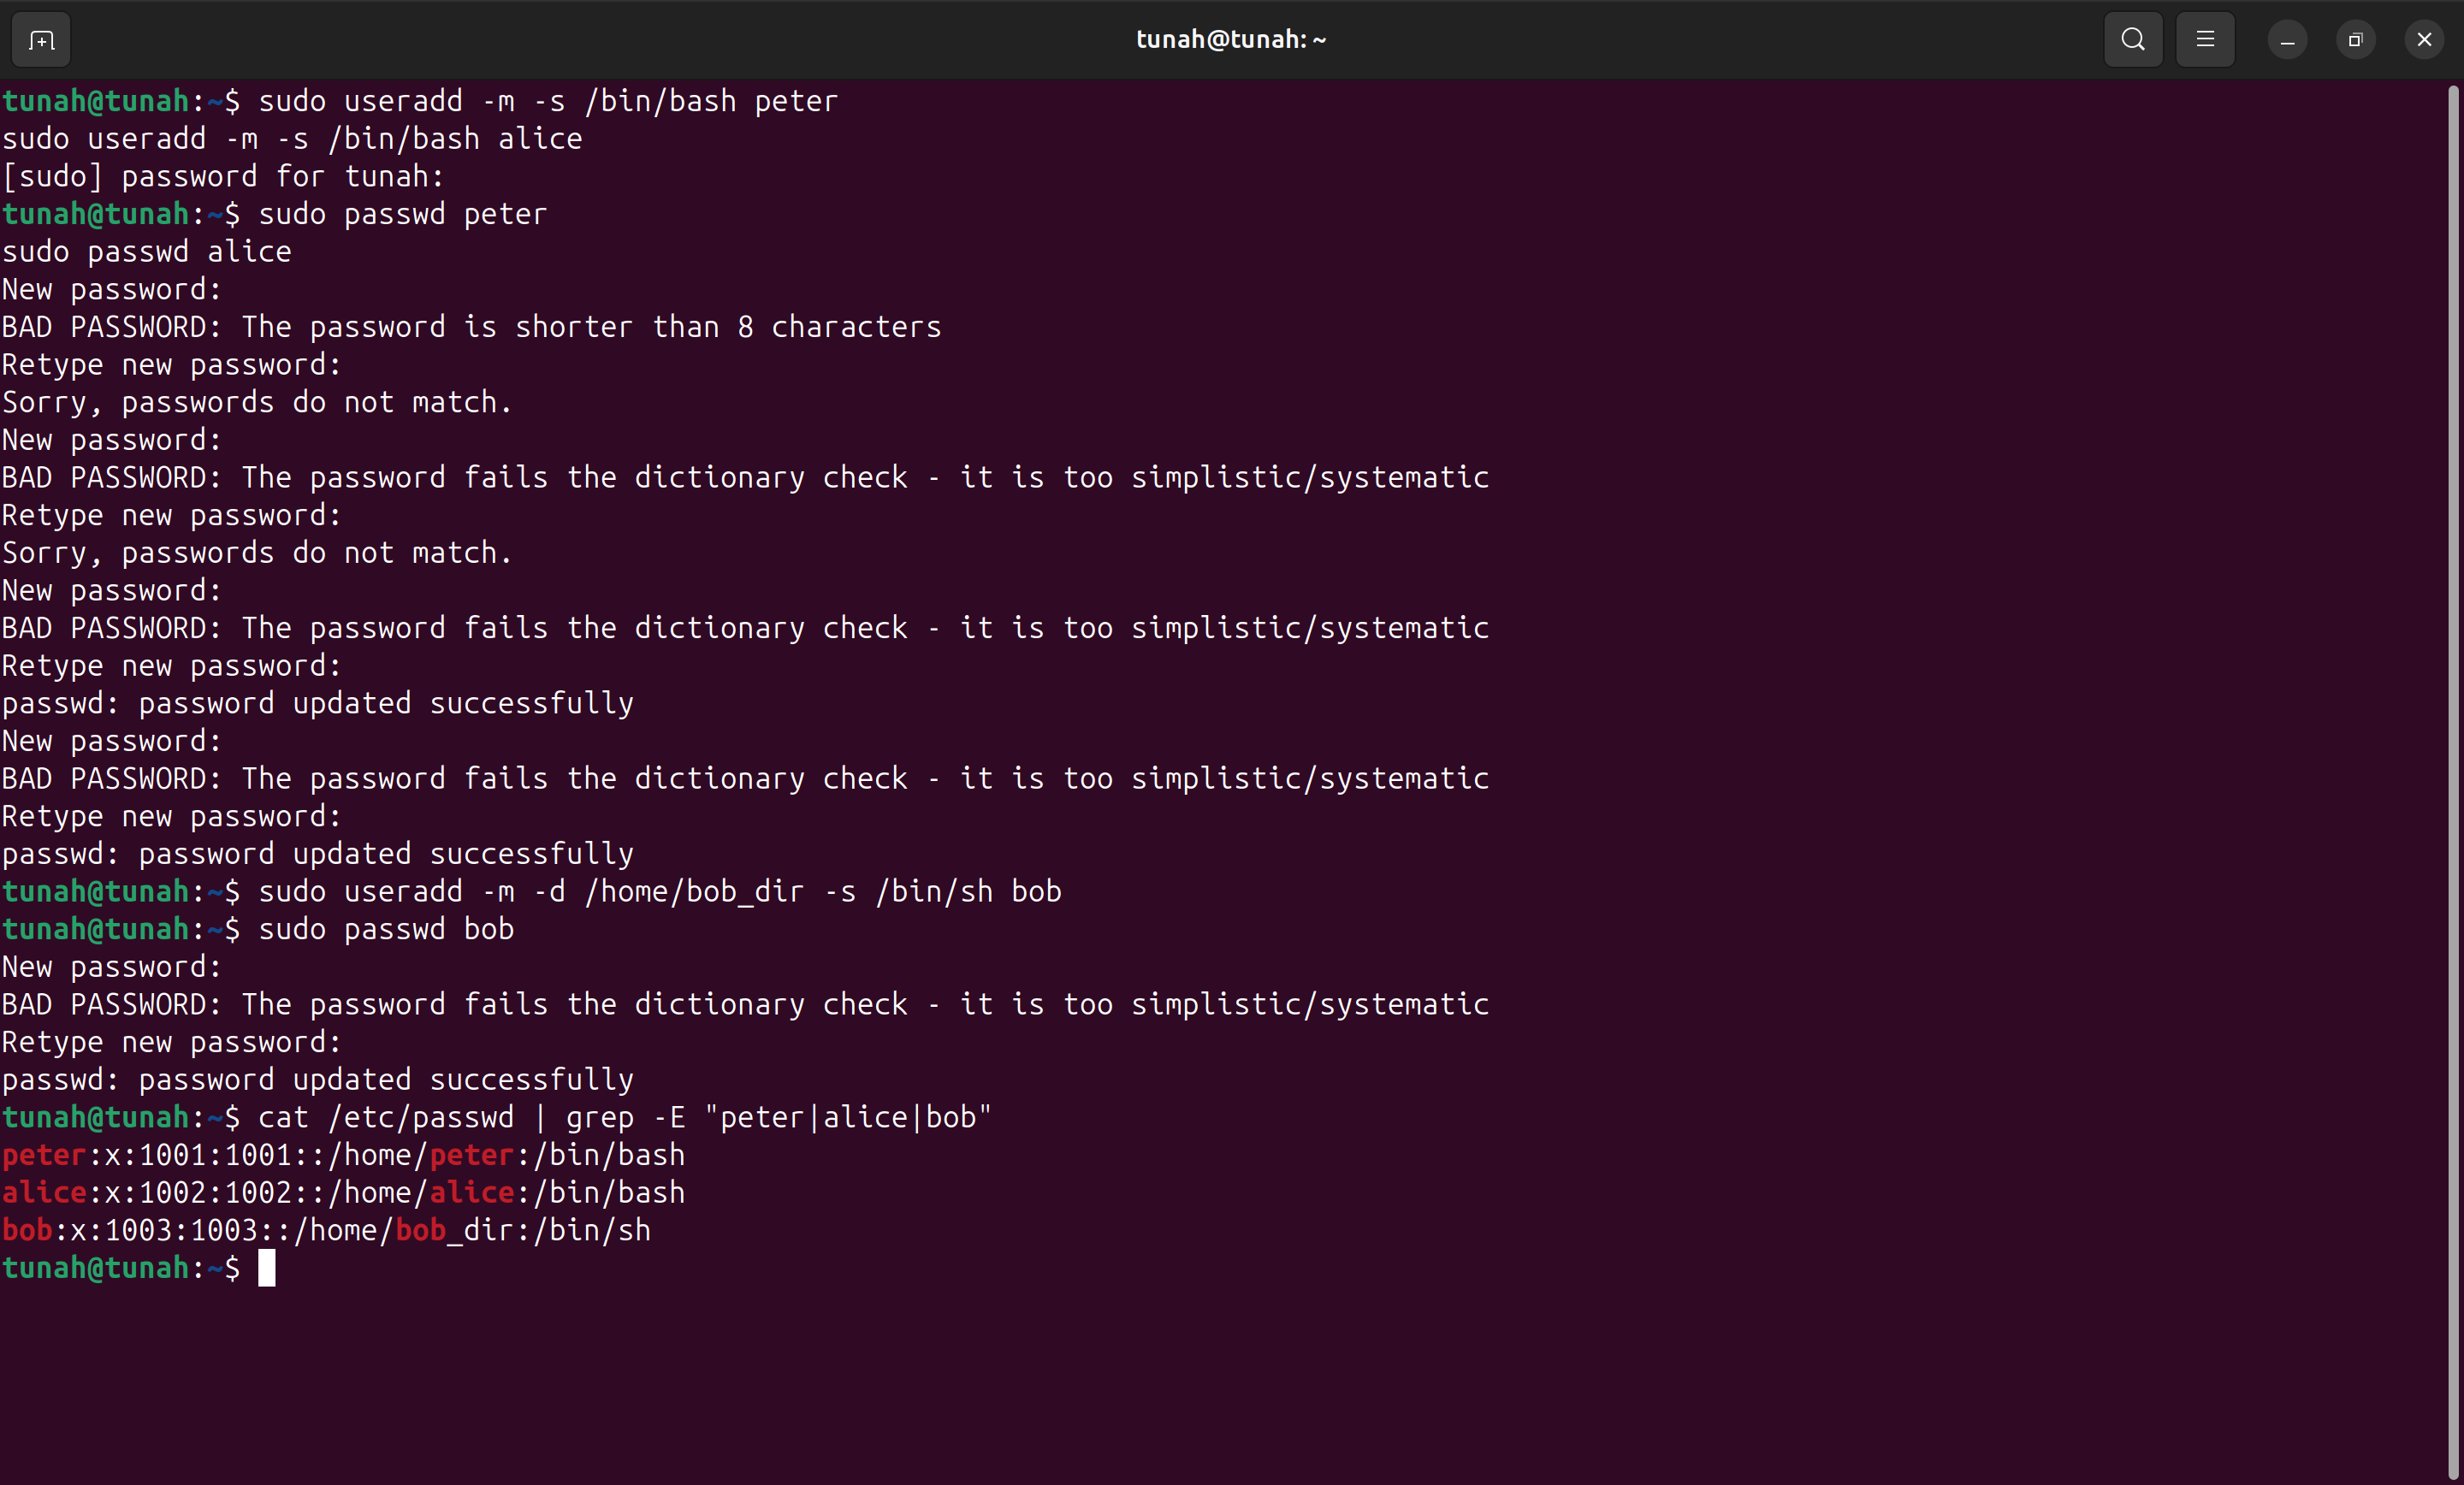
\includegraphics[width=\textwidth]{01/list-users-created.png}
        \caption{Danh sách 3 user đã tạo}
    \end{subfigure}
    \hfill
    \begin{subfigure}[b]{0.48\textwidth}
        \centering
        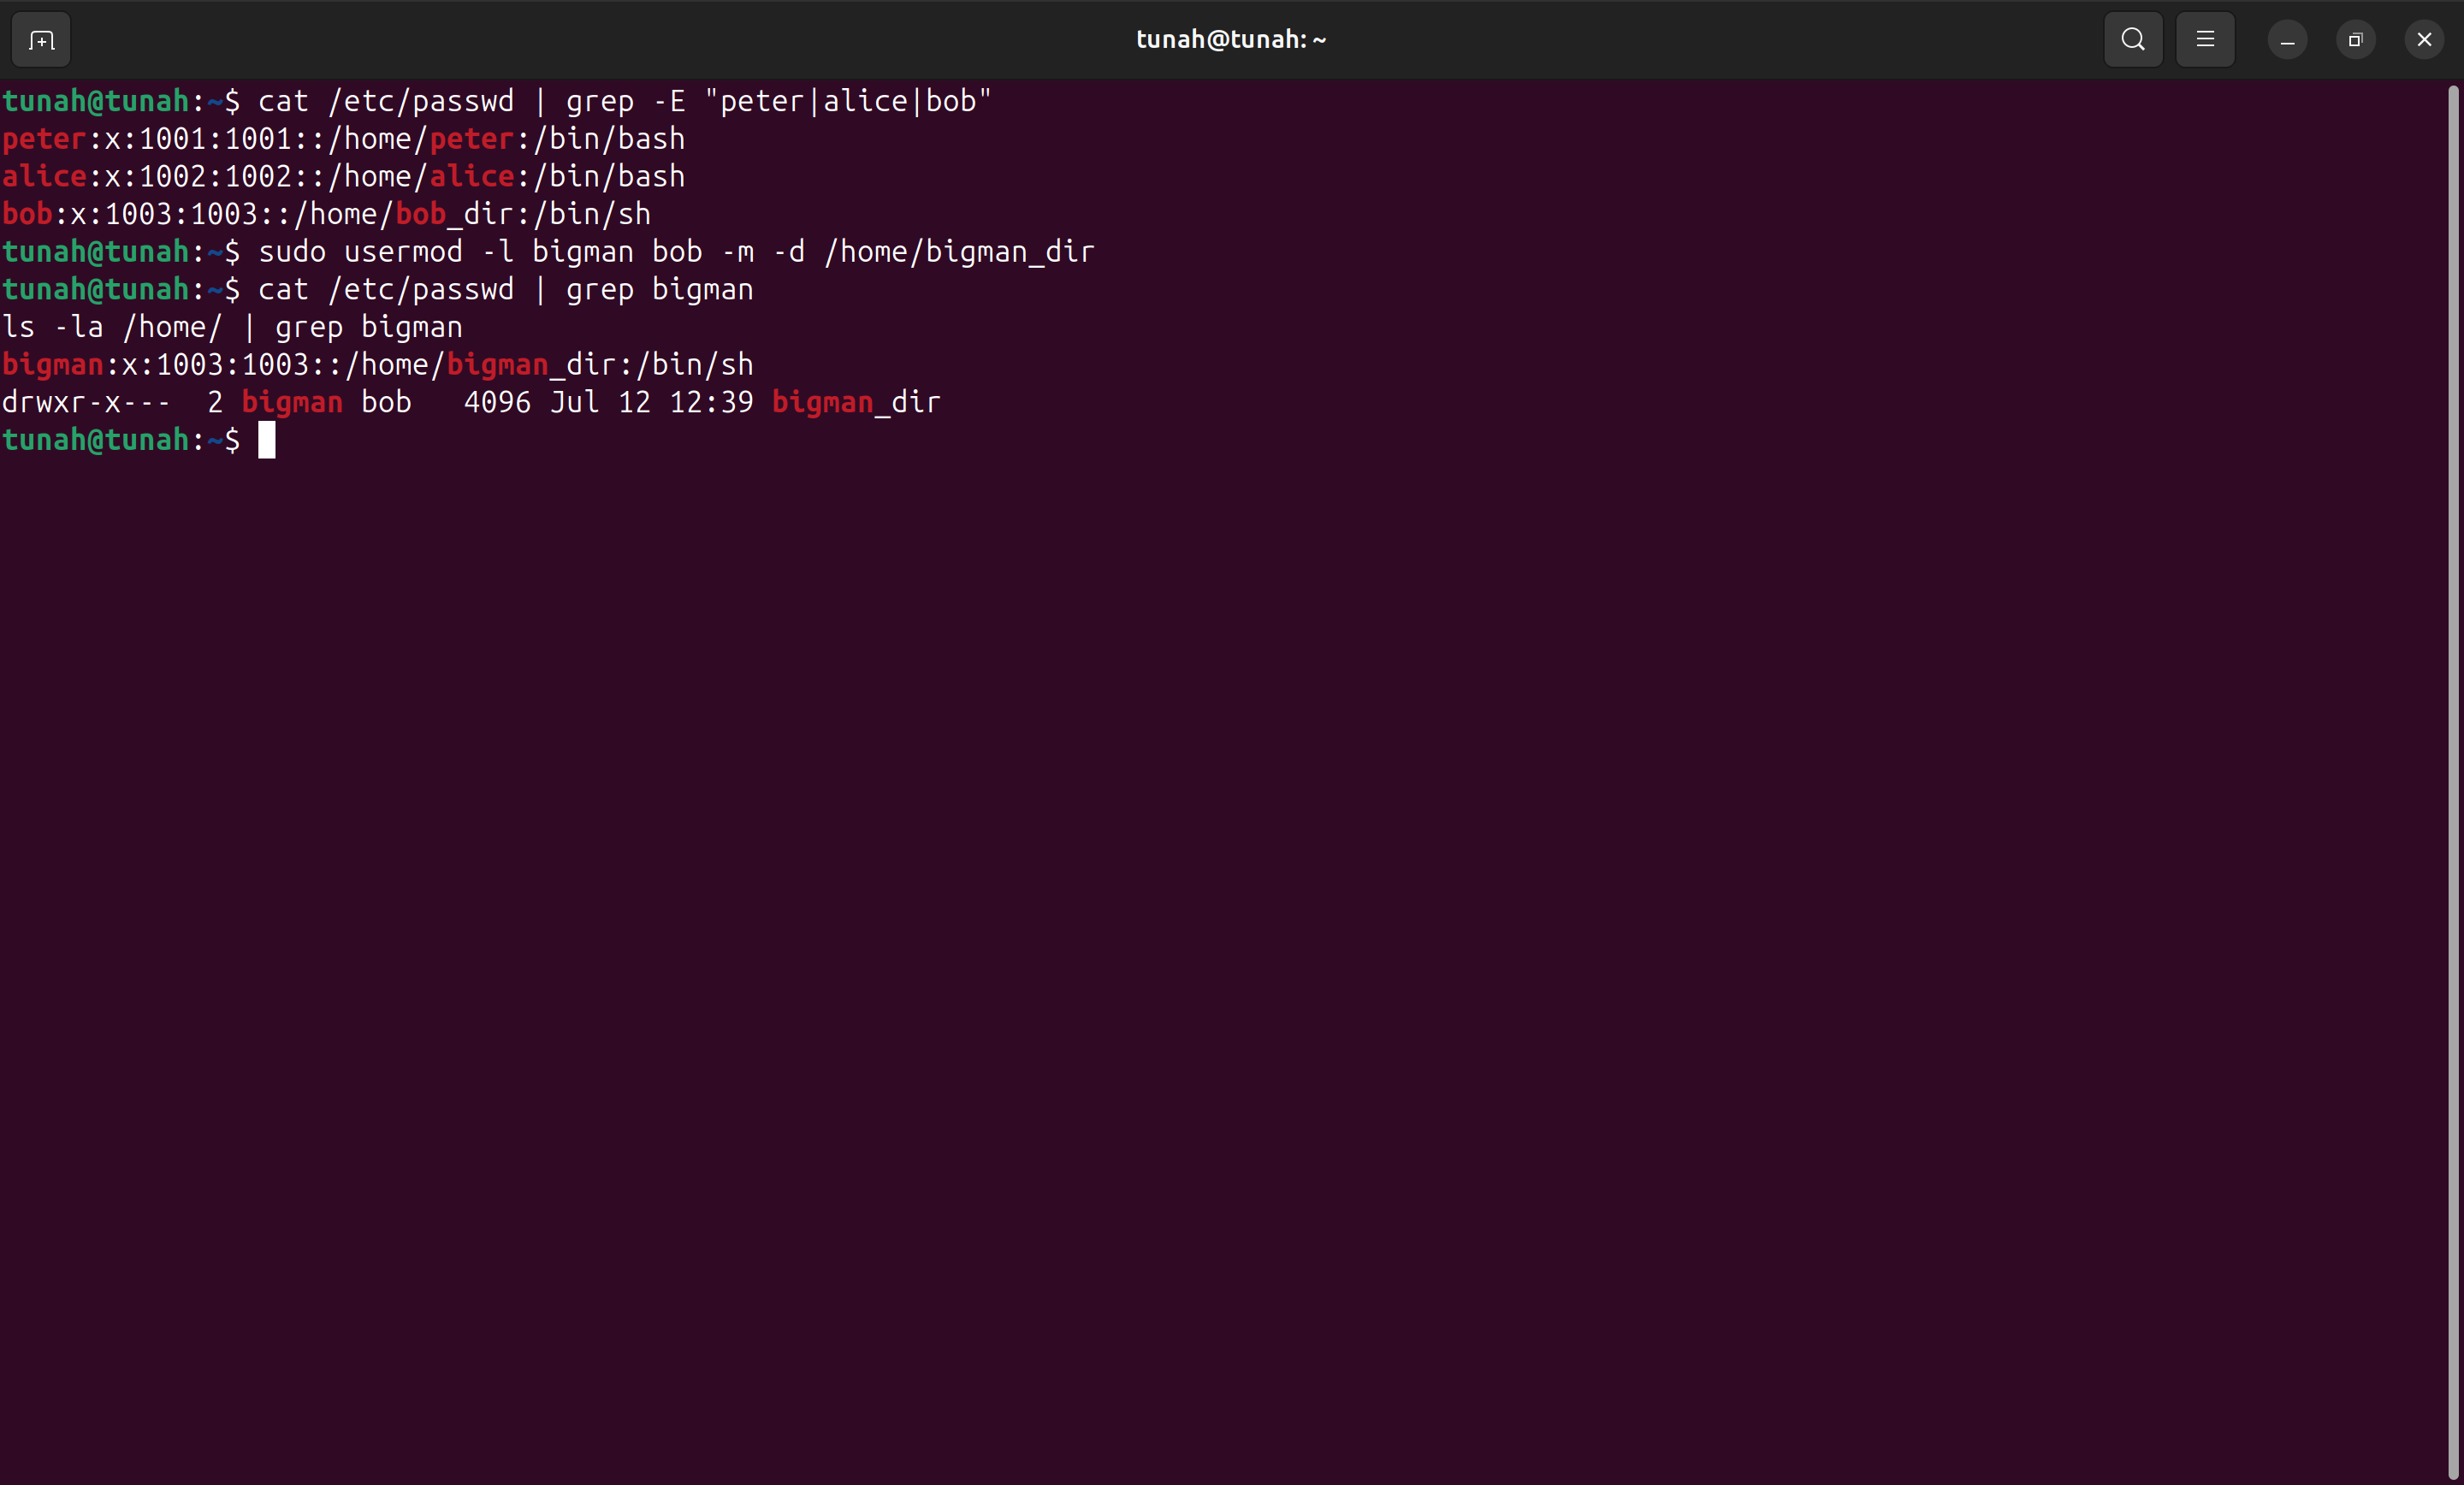
\includegraphics[width=\textwidth]{01/user-bigman-renamed.png}
        \caption{User bigman với home directory mới}
    \end{subfigure}
    
    \vspace{0.5cm}
    \begin{subfigure}[b]{0.48\textwidth}
        \centering
        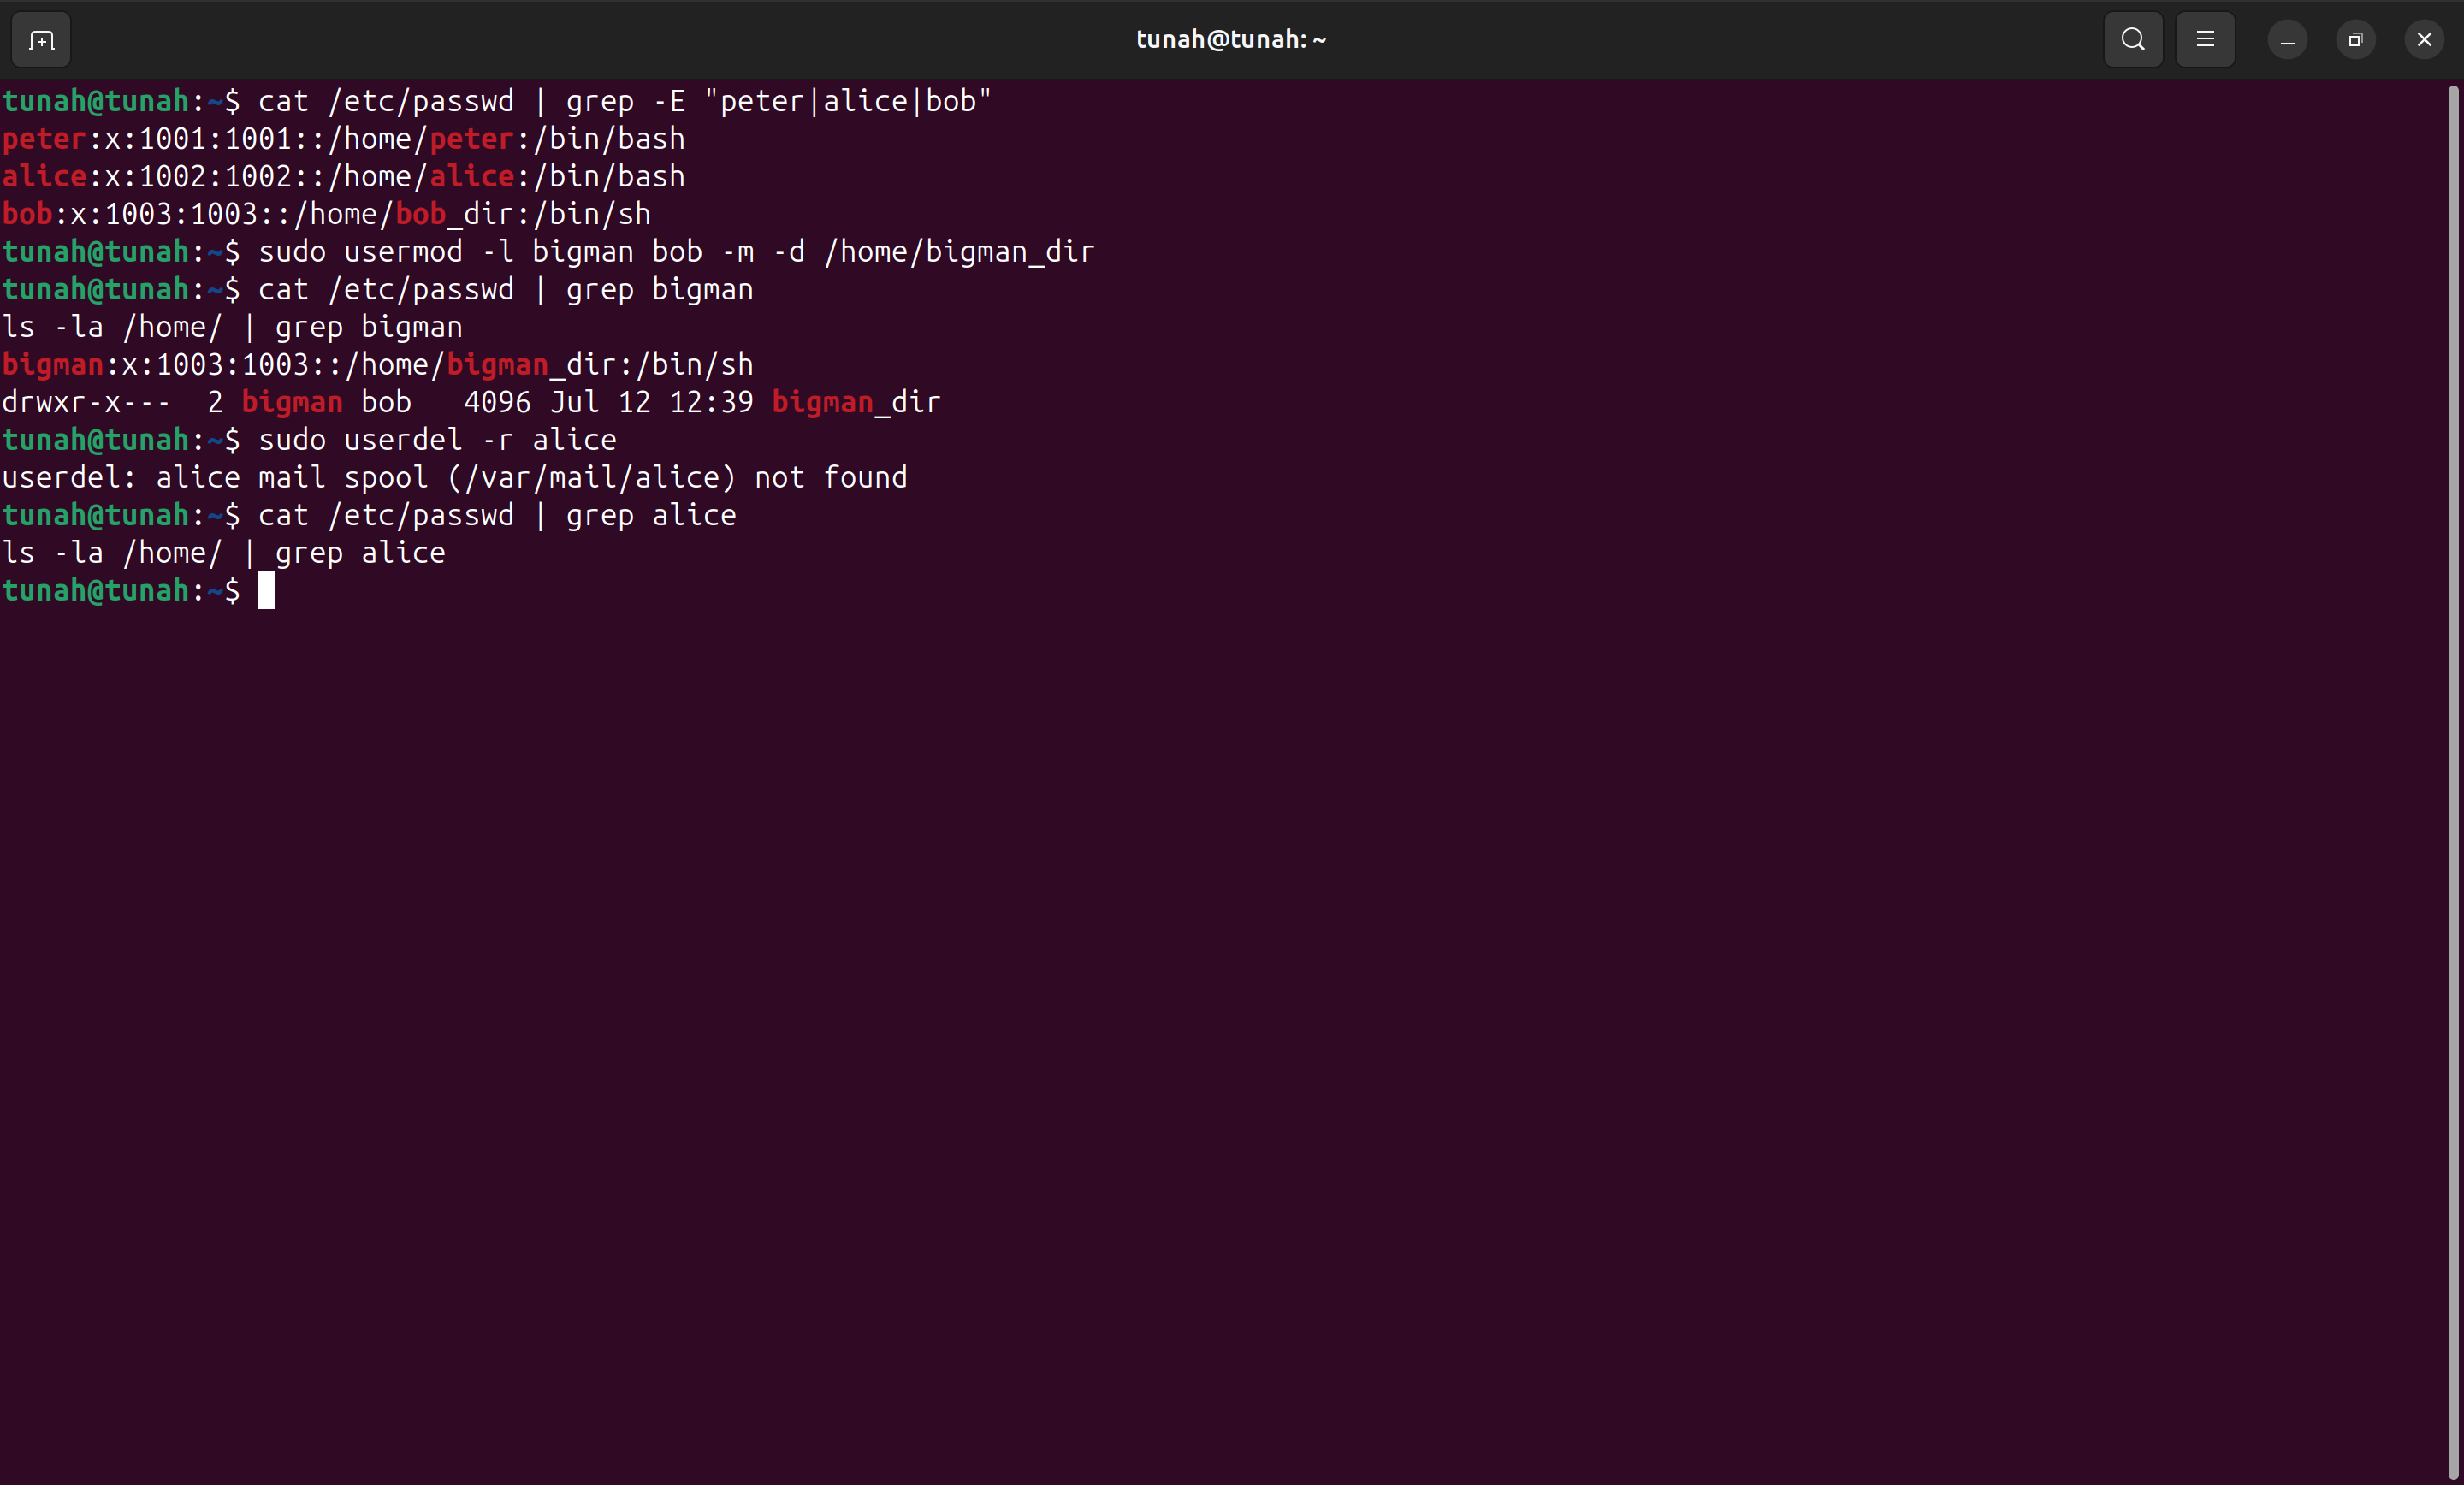
\includegraphics[width=\textwidth]{01/user-alice-deleted.png}
        \caption{Xác nhận alice đã bị xóa}
    \end{subfigure}
    \caption{Kết quả Bài tập 1: Quản lý user}
\end{figure}


\subsection{Bài tập 2: Tạo và quản lý group}

\textbf{Cách thực hiện:}
Tạo group \texttt{tech} và thêm \texttt{peter}, \texttt{bigman}. Tạo group \texttt{marketing} và thêm \texttt{bigman}. Cuối cùng xóa group \texttt{marketing}.

\begin{lstlisting}[language=bash]
# Tao group tech va them thanh vien
sudo groupadd tech
sudo usermod -aG tech peter
sudo usermod -aG tech bigman

# Tao group marketing va them bigman
sudo groupadd marketing
sudo usermod -aG marketing bigman

# Xoa group marketing
sudo groupdel marketing
\end{lstlisting}

\textbf{Kết quả:}
Thành viên được cấp group đúng như chỉ định và group \texttt{marketing} đã được gỡ bỏ thành công khỏi hệ thống.

\begin{figure}[H]
    \centering
    \begin{subfigure}[b]{0.48\textwidth}
        \centering
        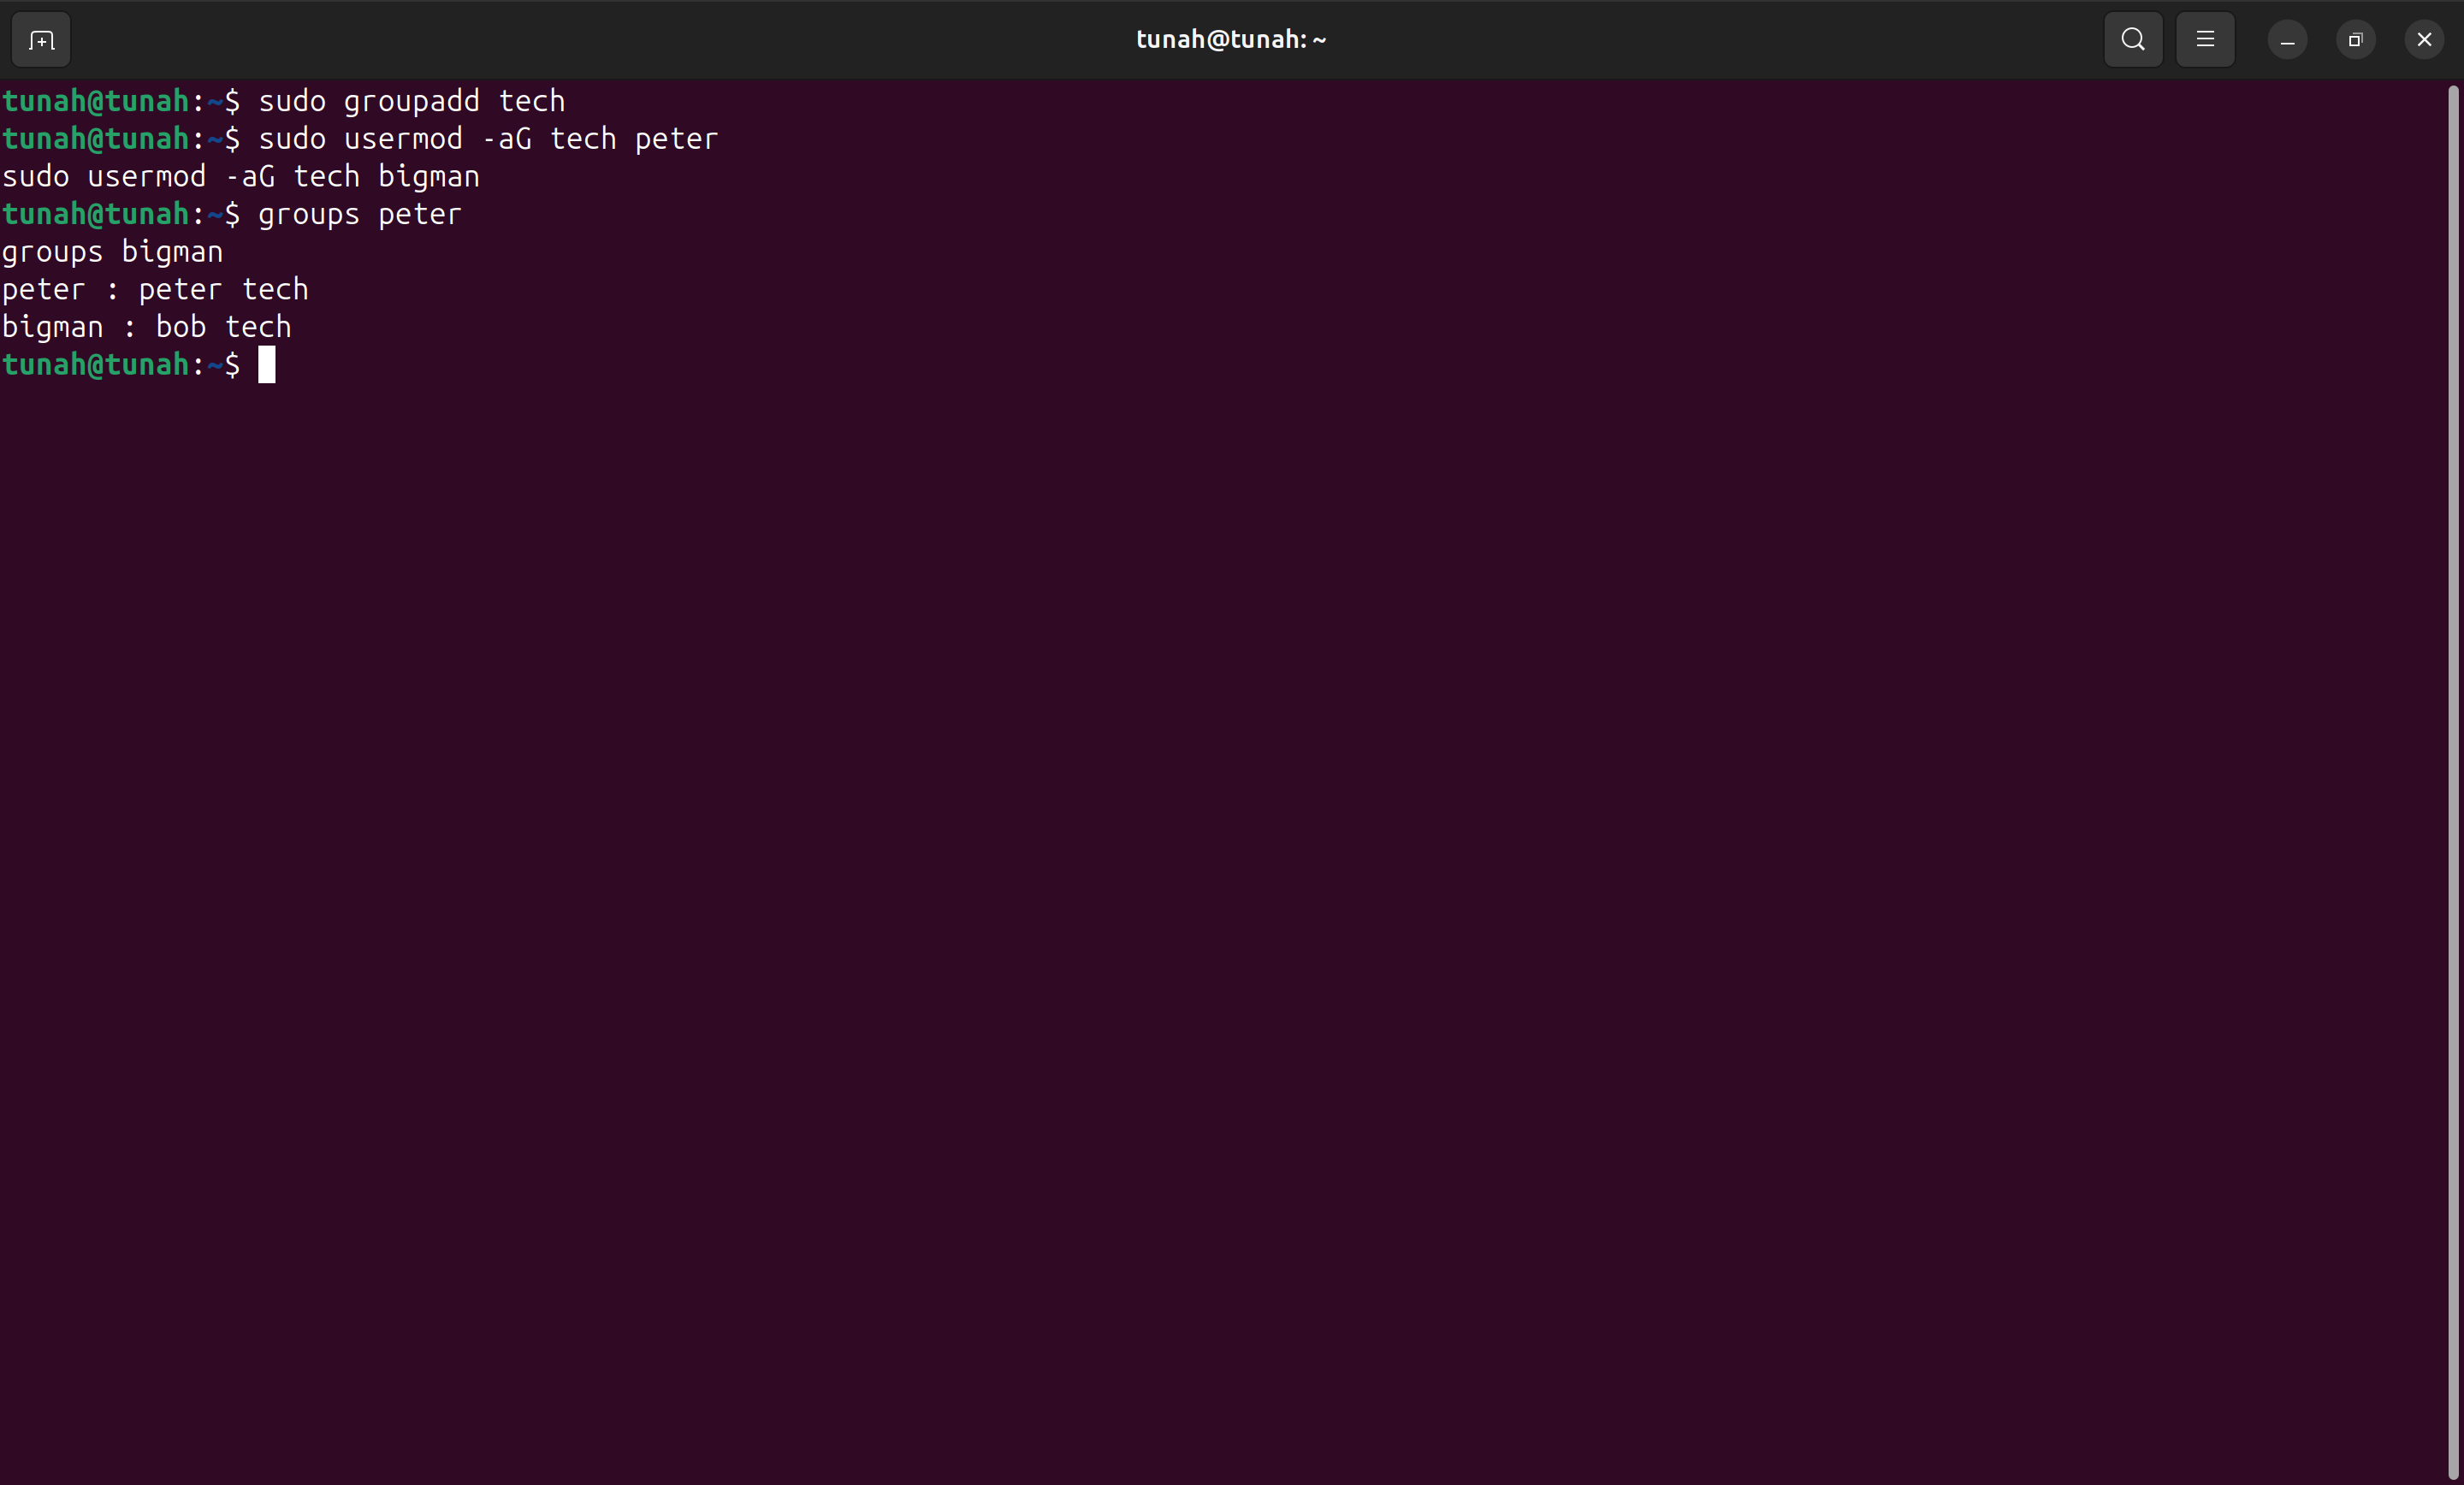
\includegraphics[width=\textwidth]{01/group-tech-members.png}
        \caption{peter và bigman thuộc group tech}
    \end{subfigure}
    \hfill
    \begin{subfigure}[b]{0.48\textwidth}
        \centering
        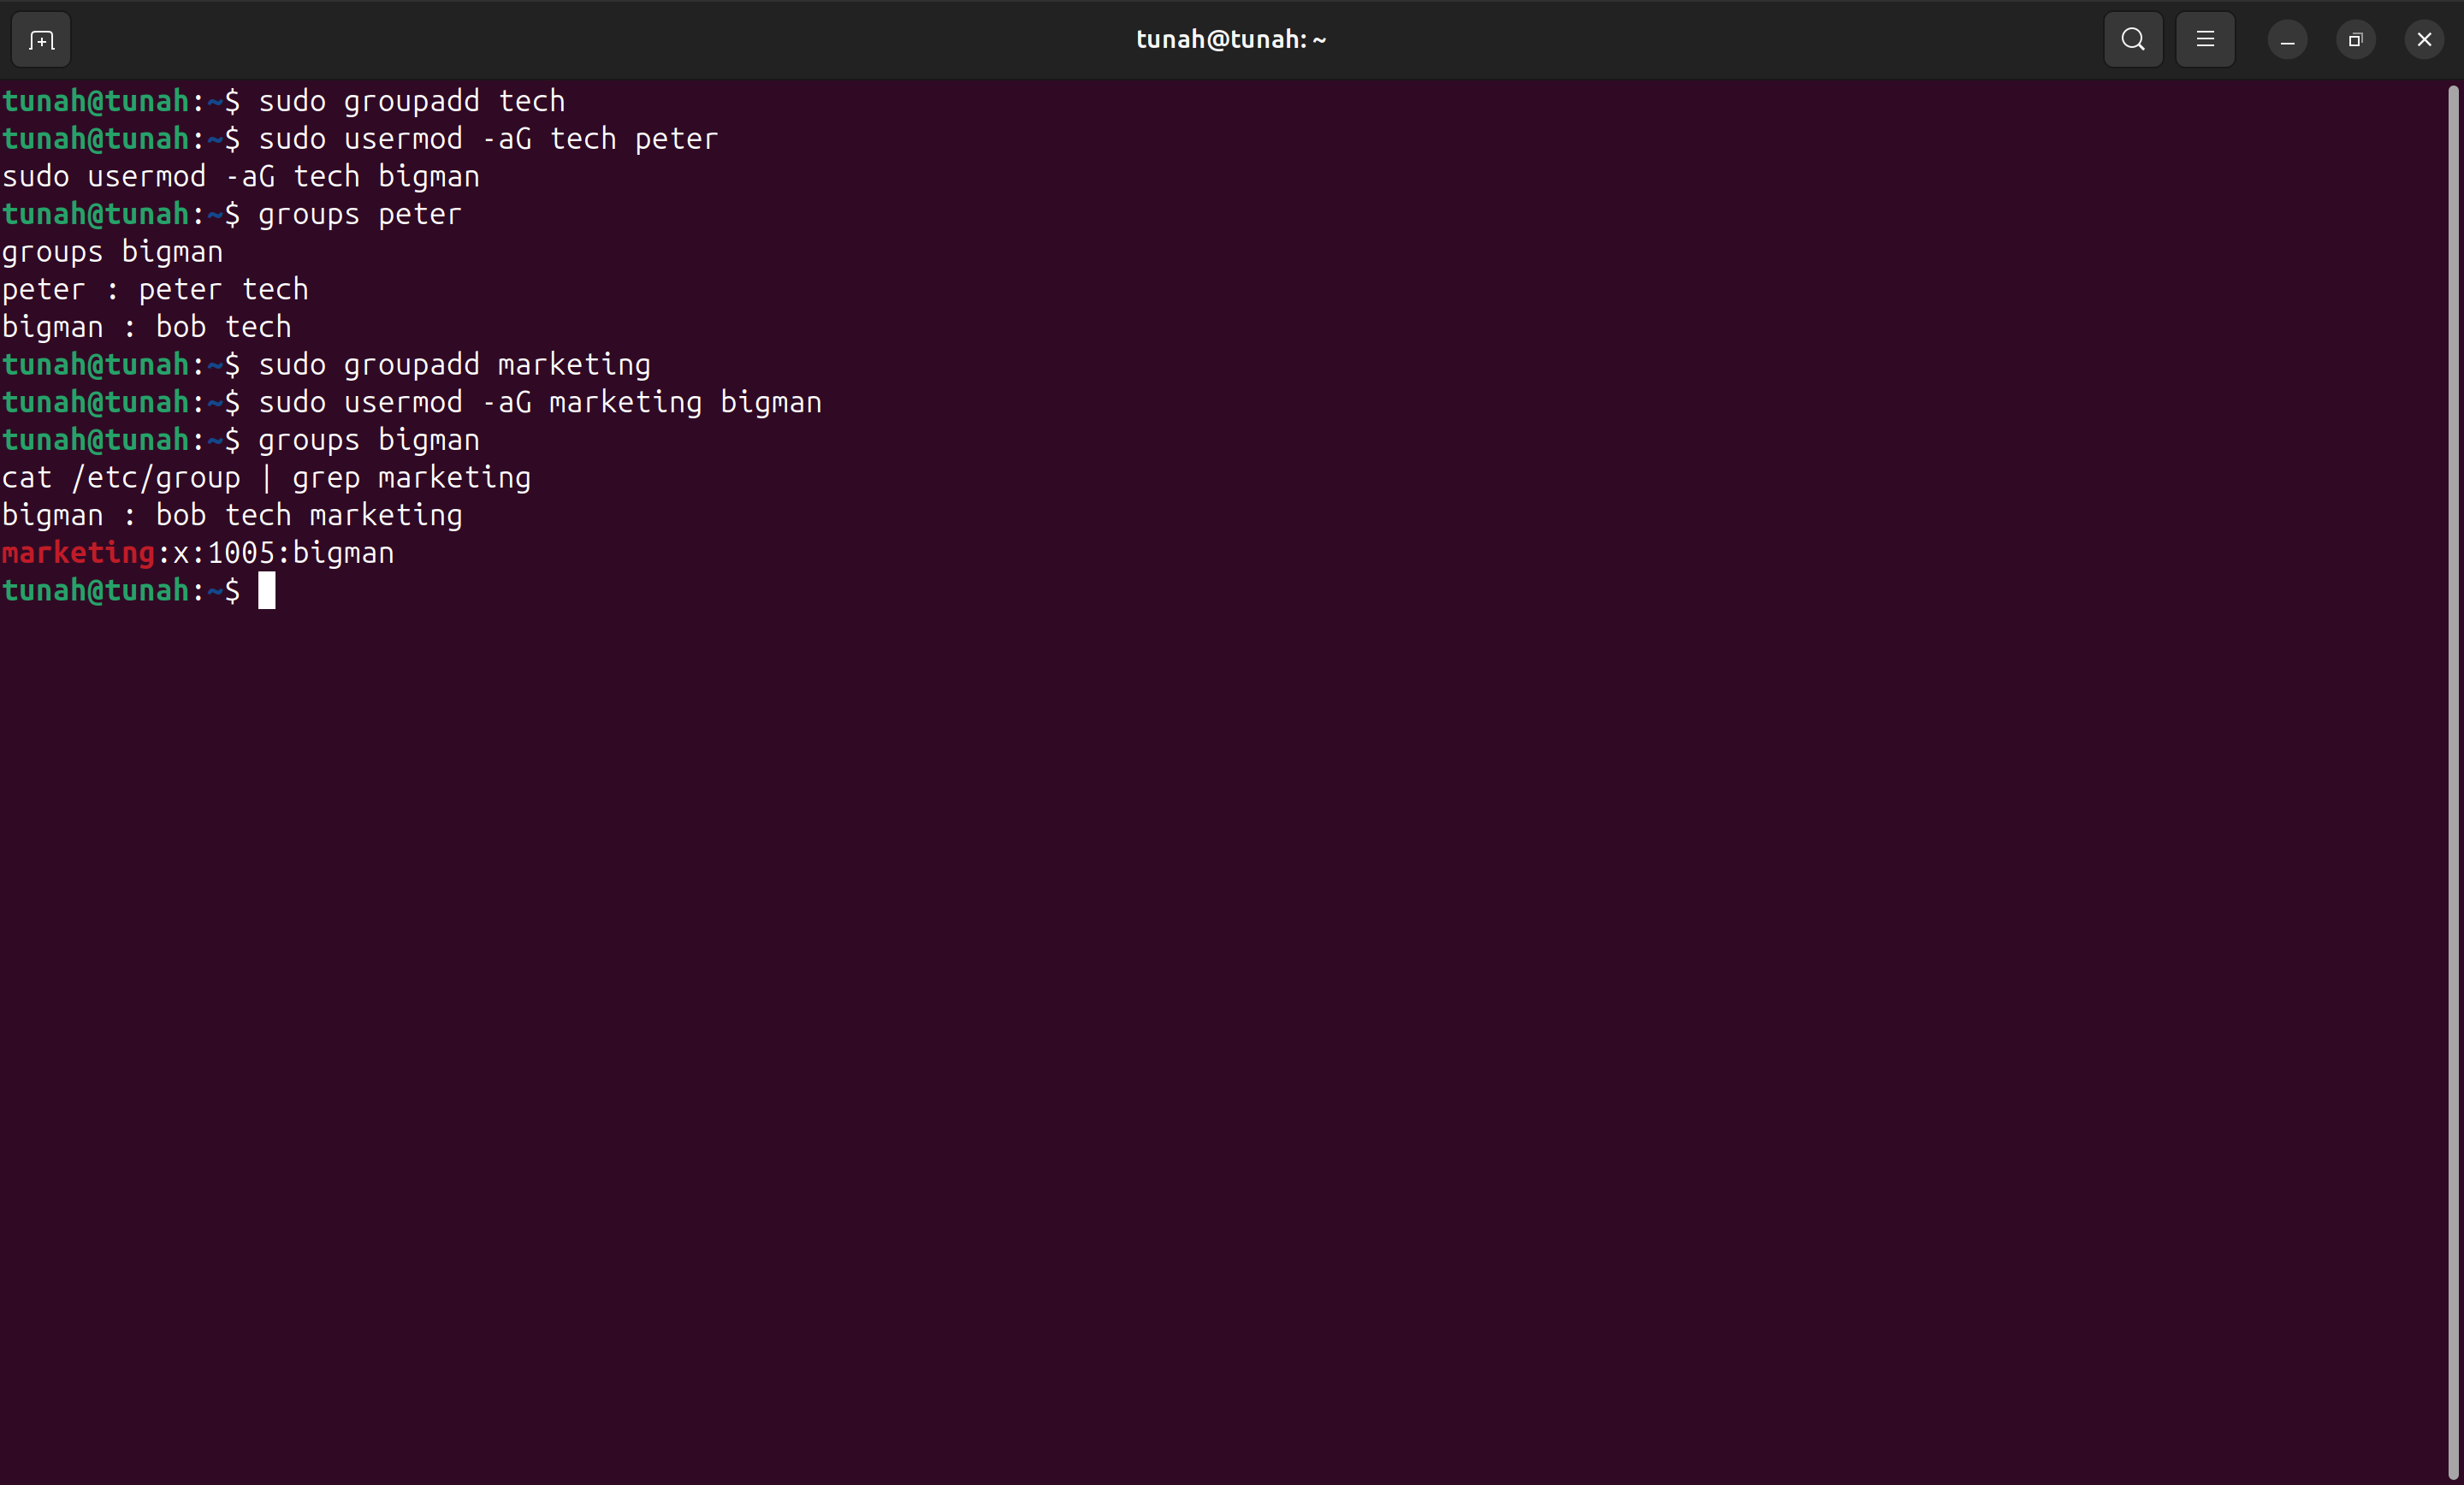
\includegraphics[width=\textwidth]{01/group-marketing-added.png}
        \caption{bigman thuộc group marketing}
    \end{subfigure}
    
    \vspace{0.5cm}
    \begin{subfigure}[b]{0.48\textwidth}
        \centering
        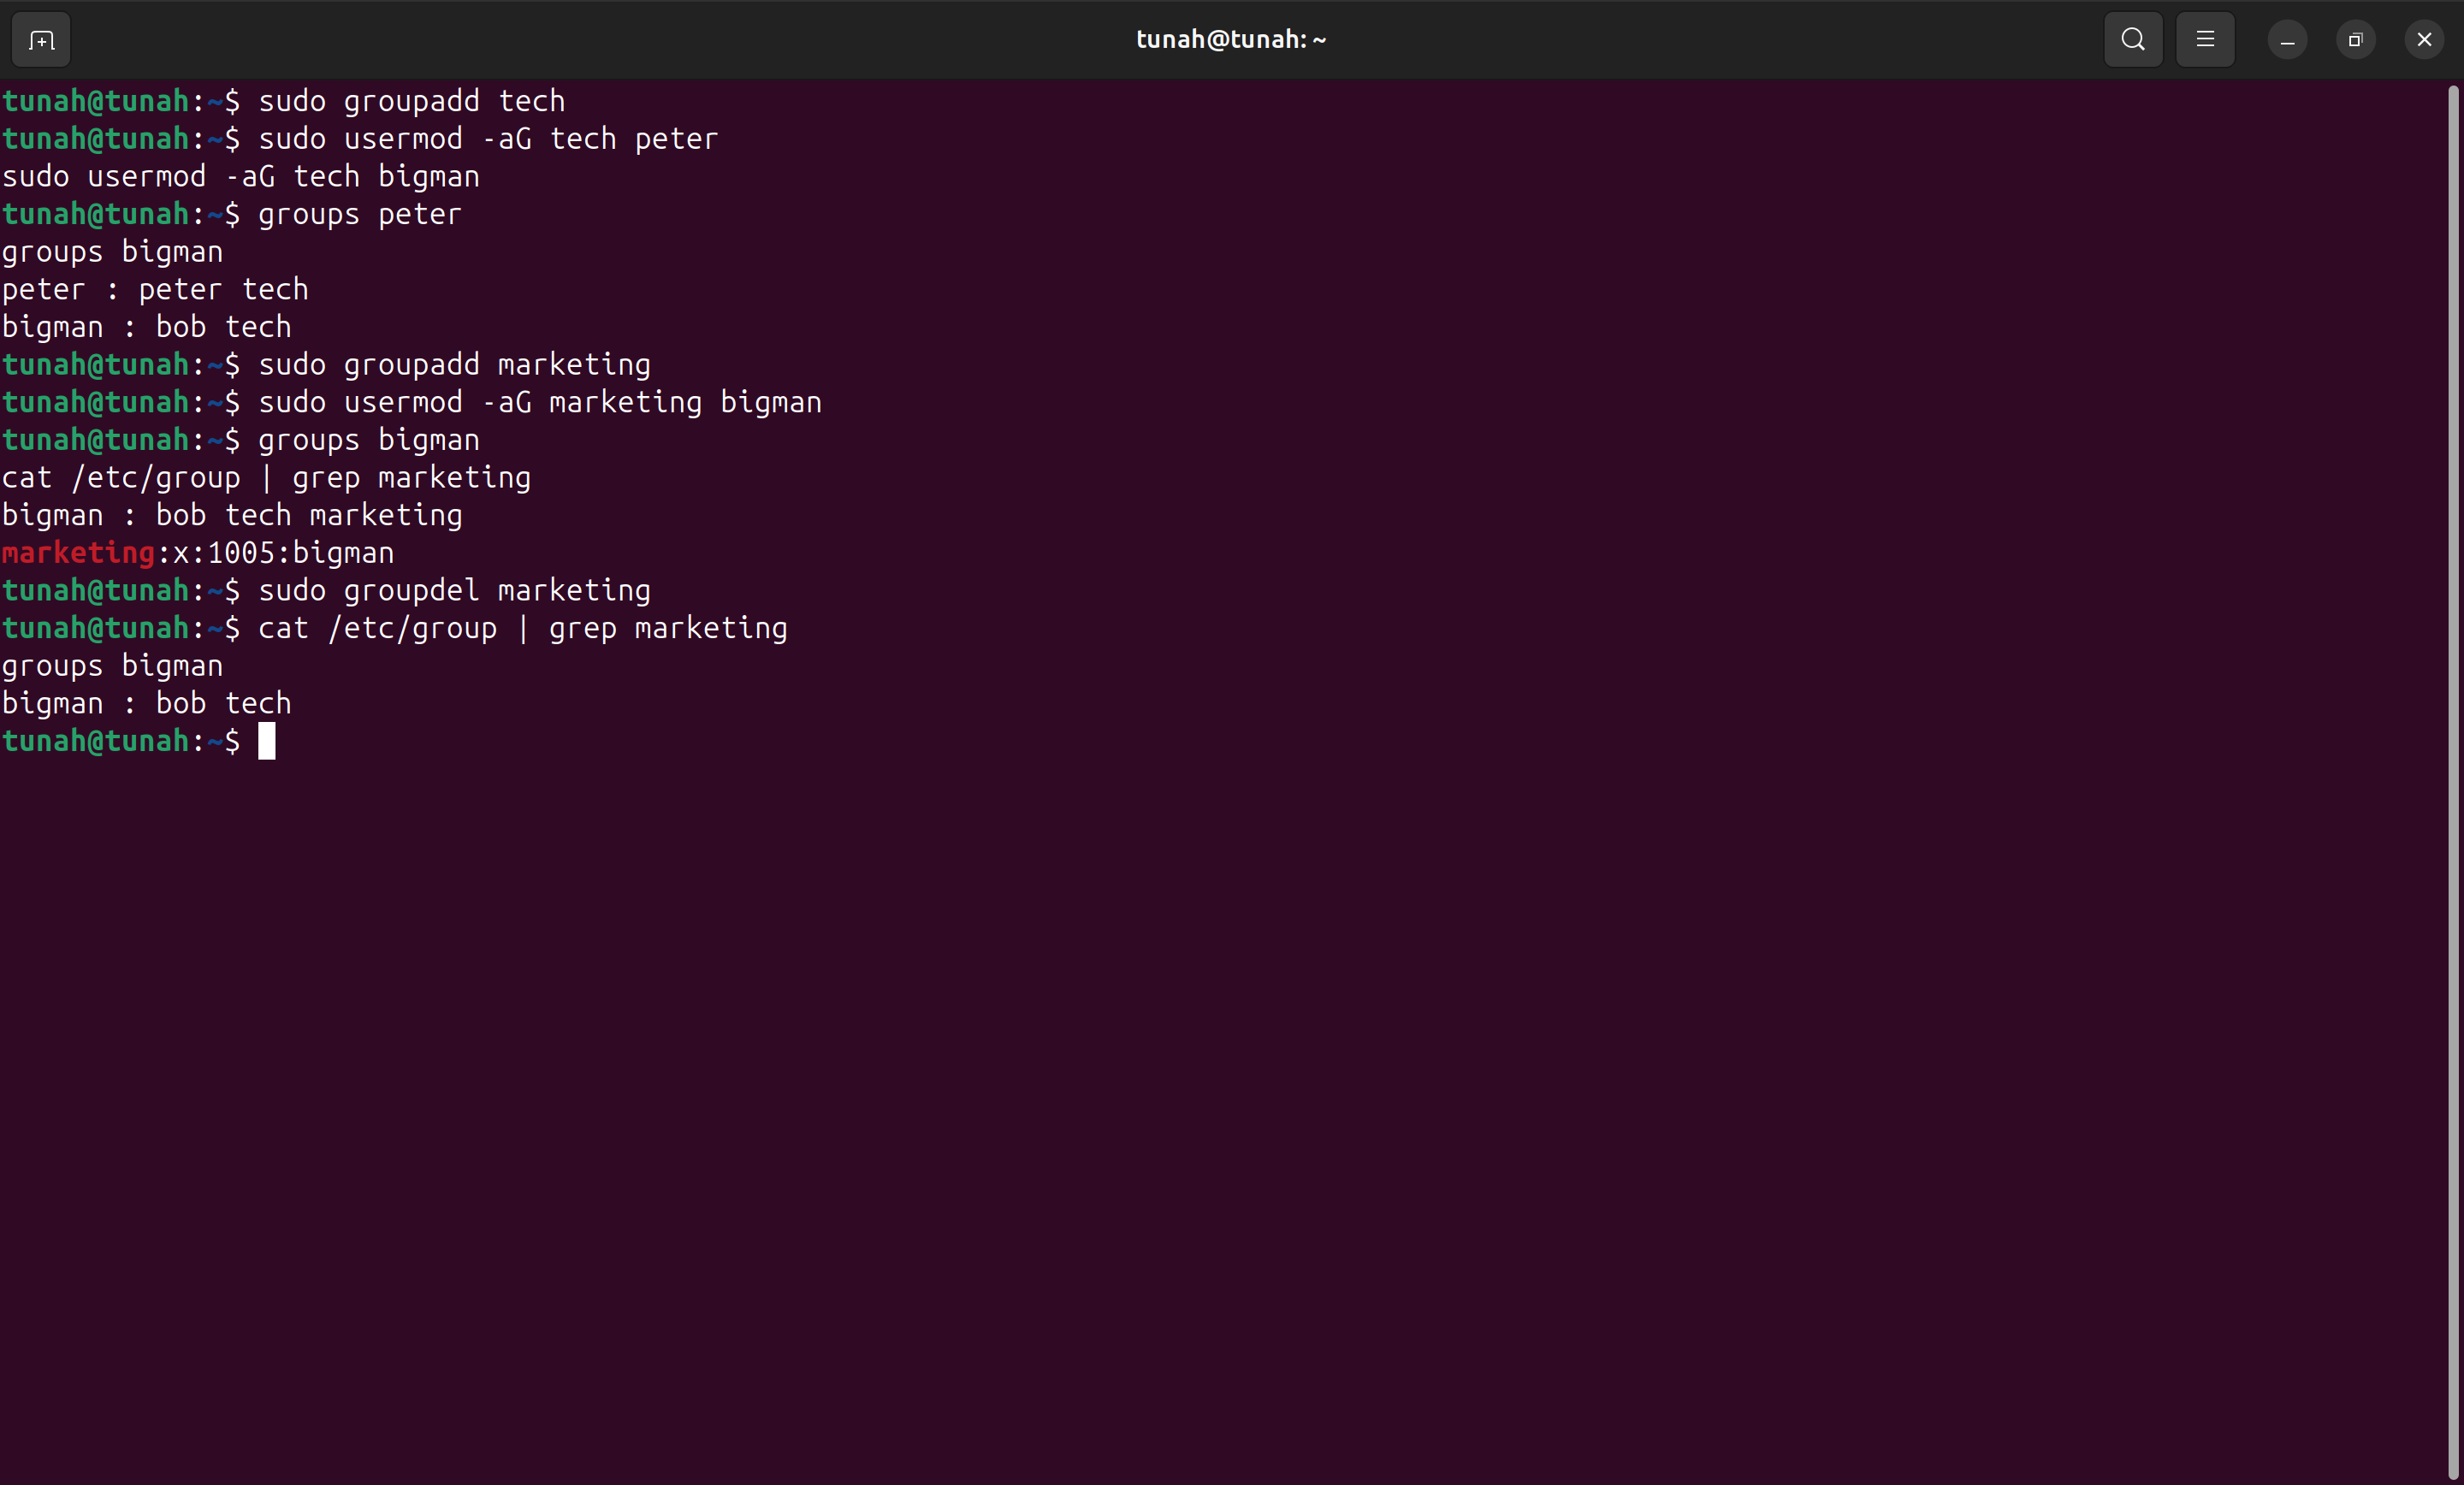
\includegraphics[width=\textwidth]{01/group-marketing-deleted.png}
        \caption{Xác nhận group marketing đã bị xóa}
    \end{subfigure}
    \caption{Kết quả Bài tập 2: Quản lý group}
\end{figure}

\section{Quản lý quyền truy cập (Permissions)}

\subsection{Bài tập 1: Thay đổi quyền bằng ký hiệu (Symbolic mode)}

\textbf{Cách thực hiện:}
Tạo tập tin \texttt{practice.txt}. Thiết lập quyền cho chủ sở hữu (đọc, ghi), nhóm (đọc) và người dùng khác (đọc). Sau đó thay đổi quyền để tất cả chỉ có quyền đọc.

\begin{lstlisting}[language=bash]
# Tao file
touch practice.txt

# Thiet lap quyen doc, ghi cho user va doc cho group/others
chmod u=rw,g=r,o=r practice.txt
ls -al | grep practice.txt

# Doi quyen tat ca thanh chi doc
chmod u=r practice.txt
ls -al | grep practice.txt
\end{lstlisting}

\textbf{Kết quả:}
Quyền của tập tin được thay đổi đúng với các thông số \texttt{-rw-r--r--} và \texttt{-r--r--r--}.

\begin{figure}[H]
    \centering
    \begin{subfigure}[b]{0.48\textwidth}
        \centering
        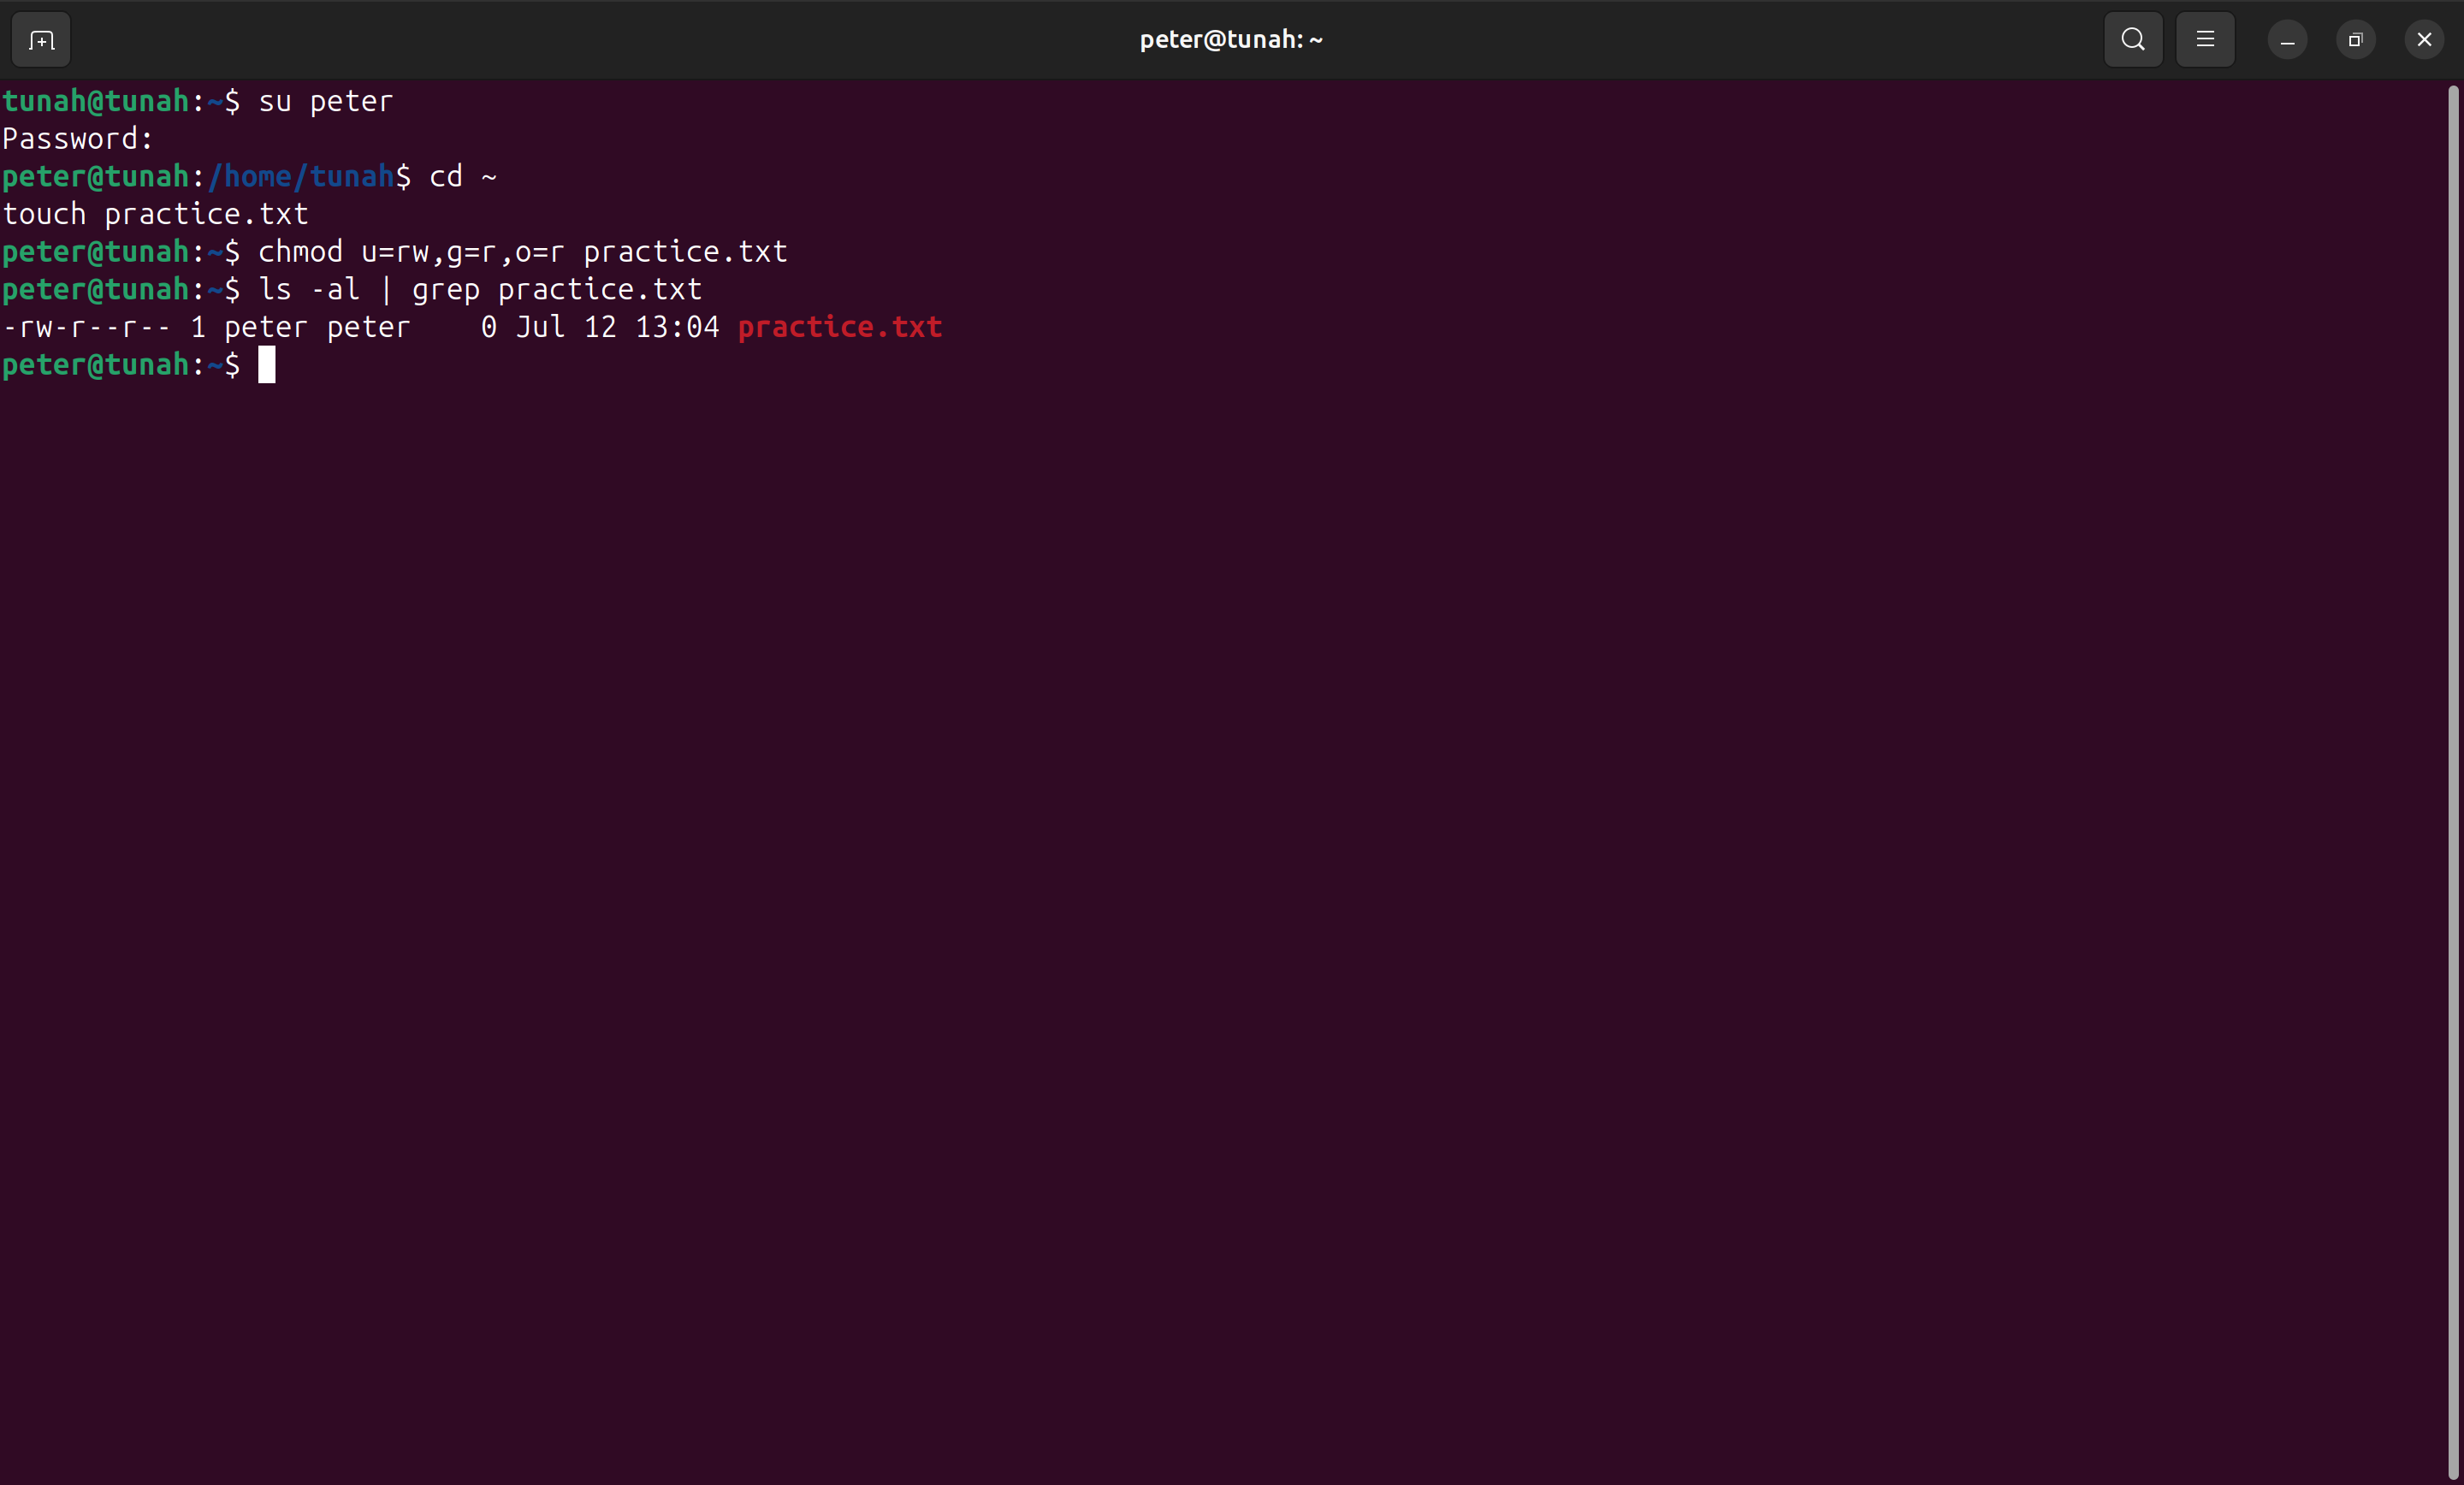
\includegraphics[width=\textwidth]{02/practice-rw-r-r.png}
        \caption{Quyền \texttt{-rw-r--r--}}
    \end{subfigure}
    \hfill
    \begin{subfigure}[b]{0.48\textwidth}
        \centering
        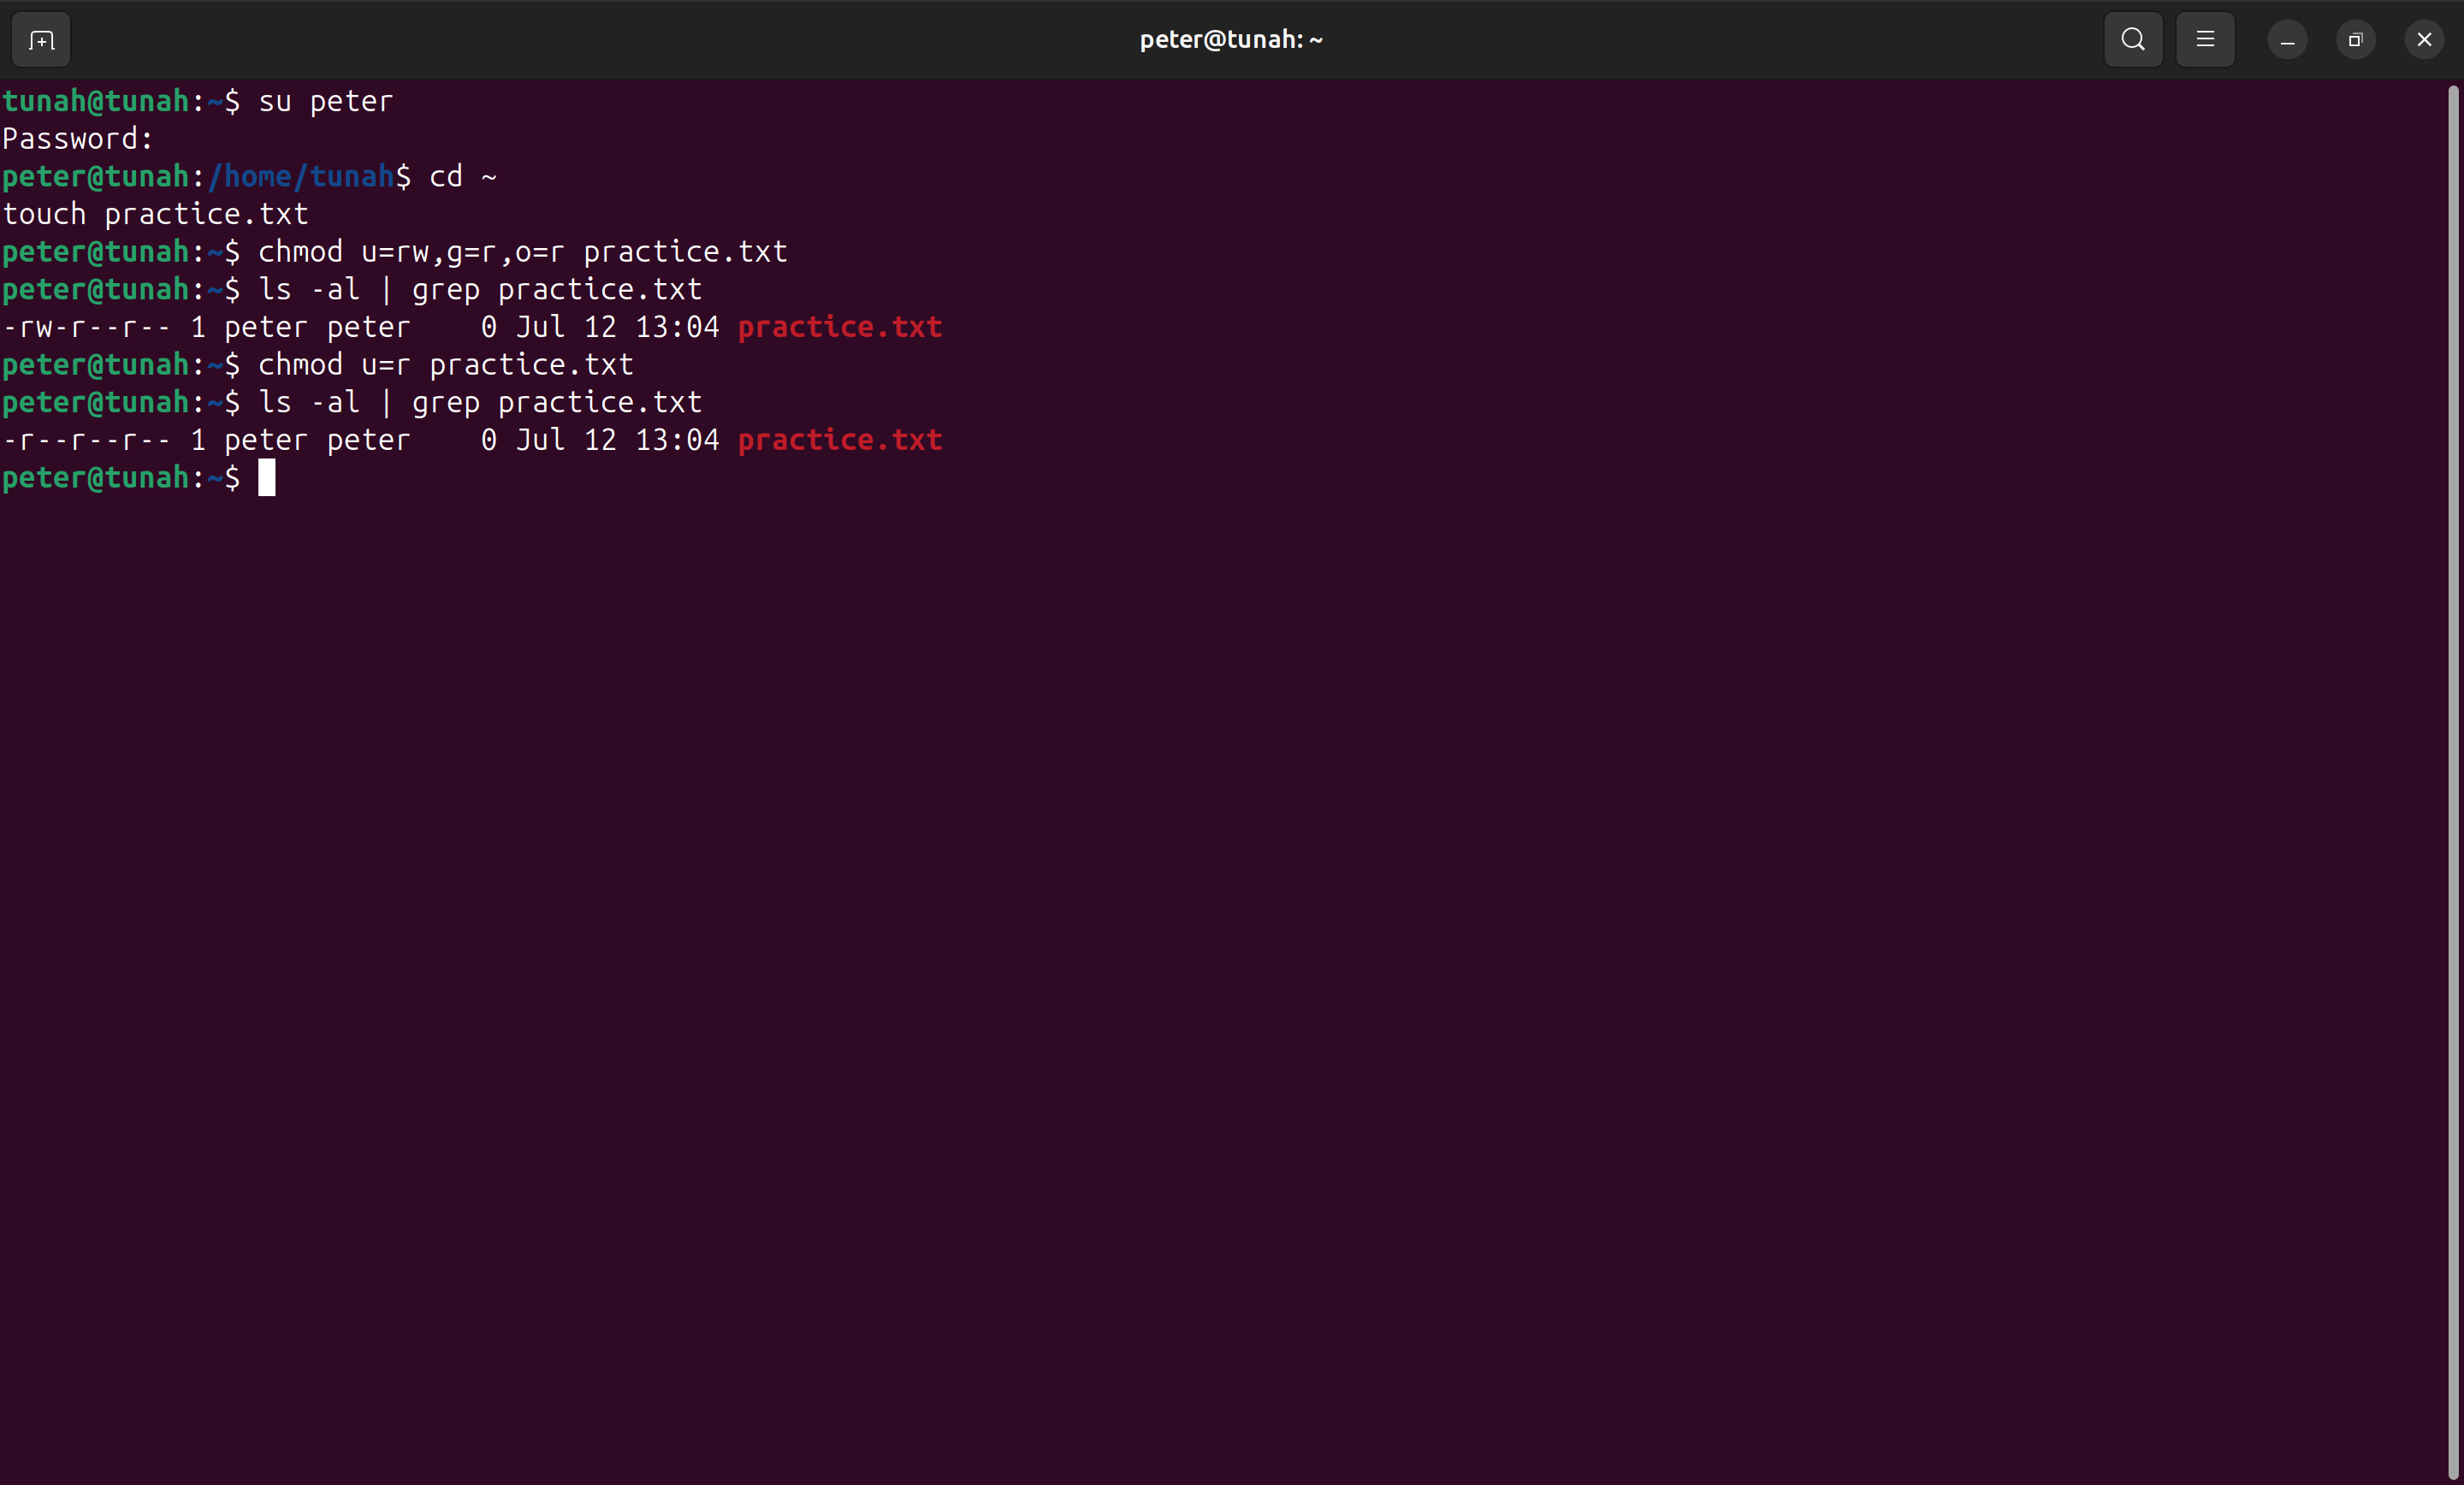
\includegraphics[width=\textwidth]{02/practice-readonly.png}
        \caption{Quyền \texttt{-r--r--r--}}
    \end{subfigure}
    \caption{Kết quả Bài tập 1: Symbolic mode}
\end{figure}

\subsection{Bài tập 2: Thay đổi quyền bằng số (Numeric mode)}

\textbf{Cách thực hiện:}
Tạo script \texttt{hello.sh} in ra "hello". Cấp quyền thực thi bằng numeric mode (744) và chạy thử.

\begin{lstlisting}[language=bash]
# Tao script hello.sh
cat <<EOF > hello.sh
#!/bin/bash
echo 'hello'
EOF

# Cap quyen 744 (rwxr--r--)
chmod 744 hello.sh
ls -al | grep hello.sh

# Thuc thi script
./hello.sh
\end{lstlisting}

\textbf{Kết quả:}
Tập tin script được cấp quyền thực thi thành công cho owner (\texttt{-rwxr--r--}) và in ra chuỗi "hello" khi chạy.

\begin{figure}[H]
    \centering
    \begin{subfigure}[b]{0.48\textwidth}
        \centering
        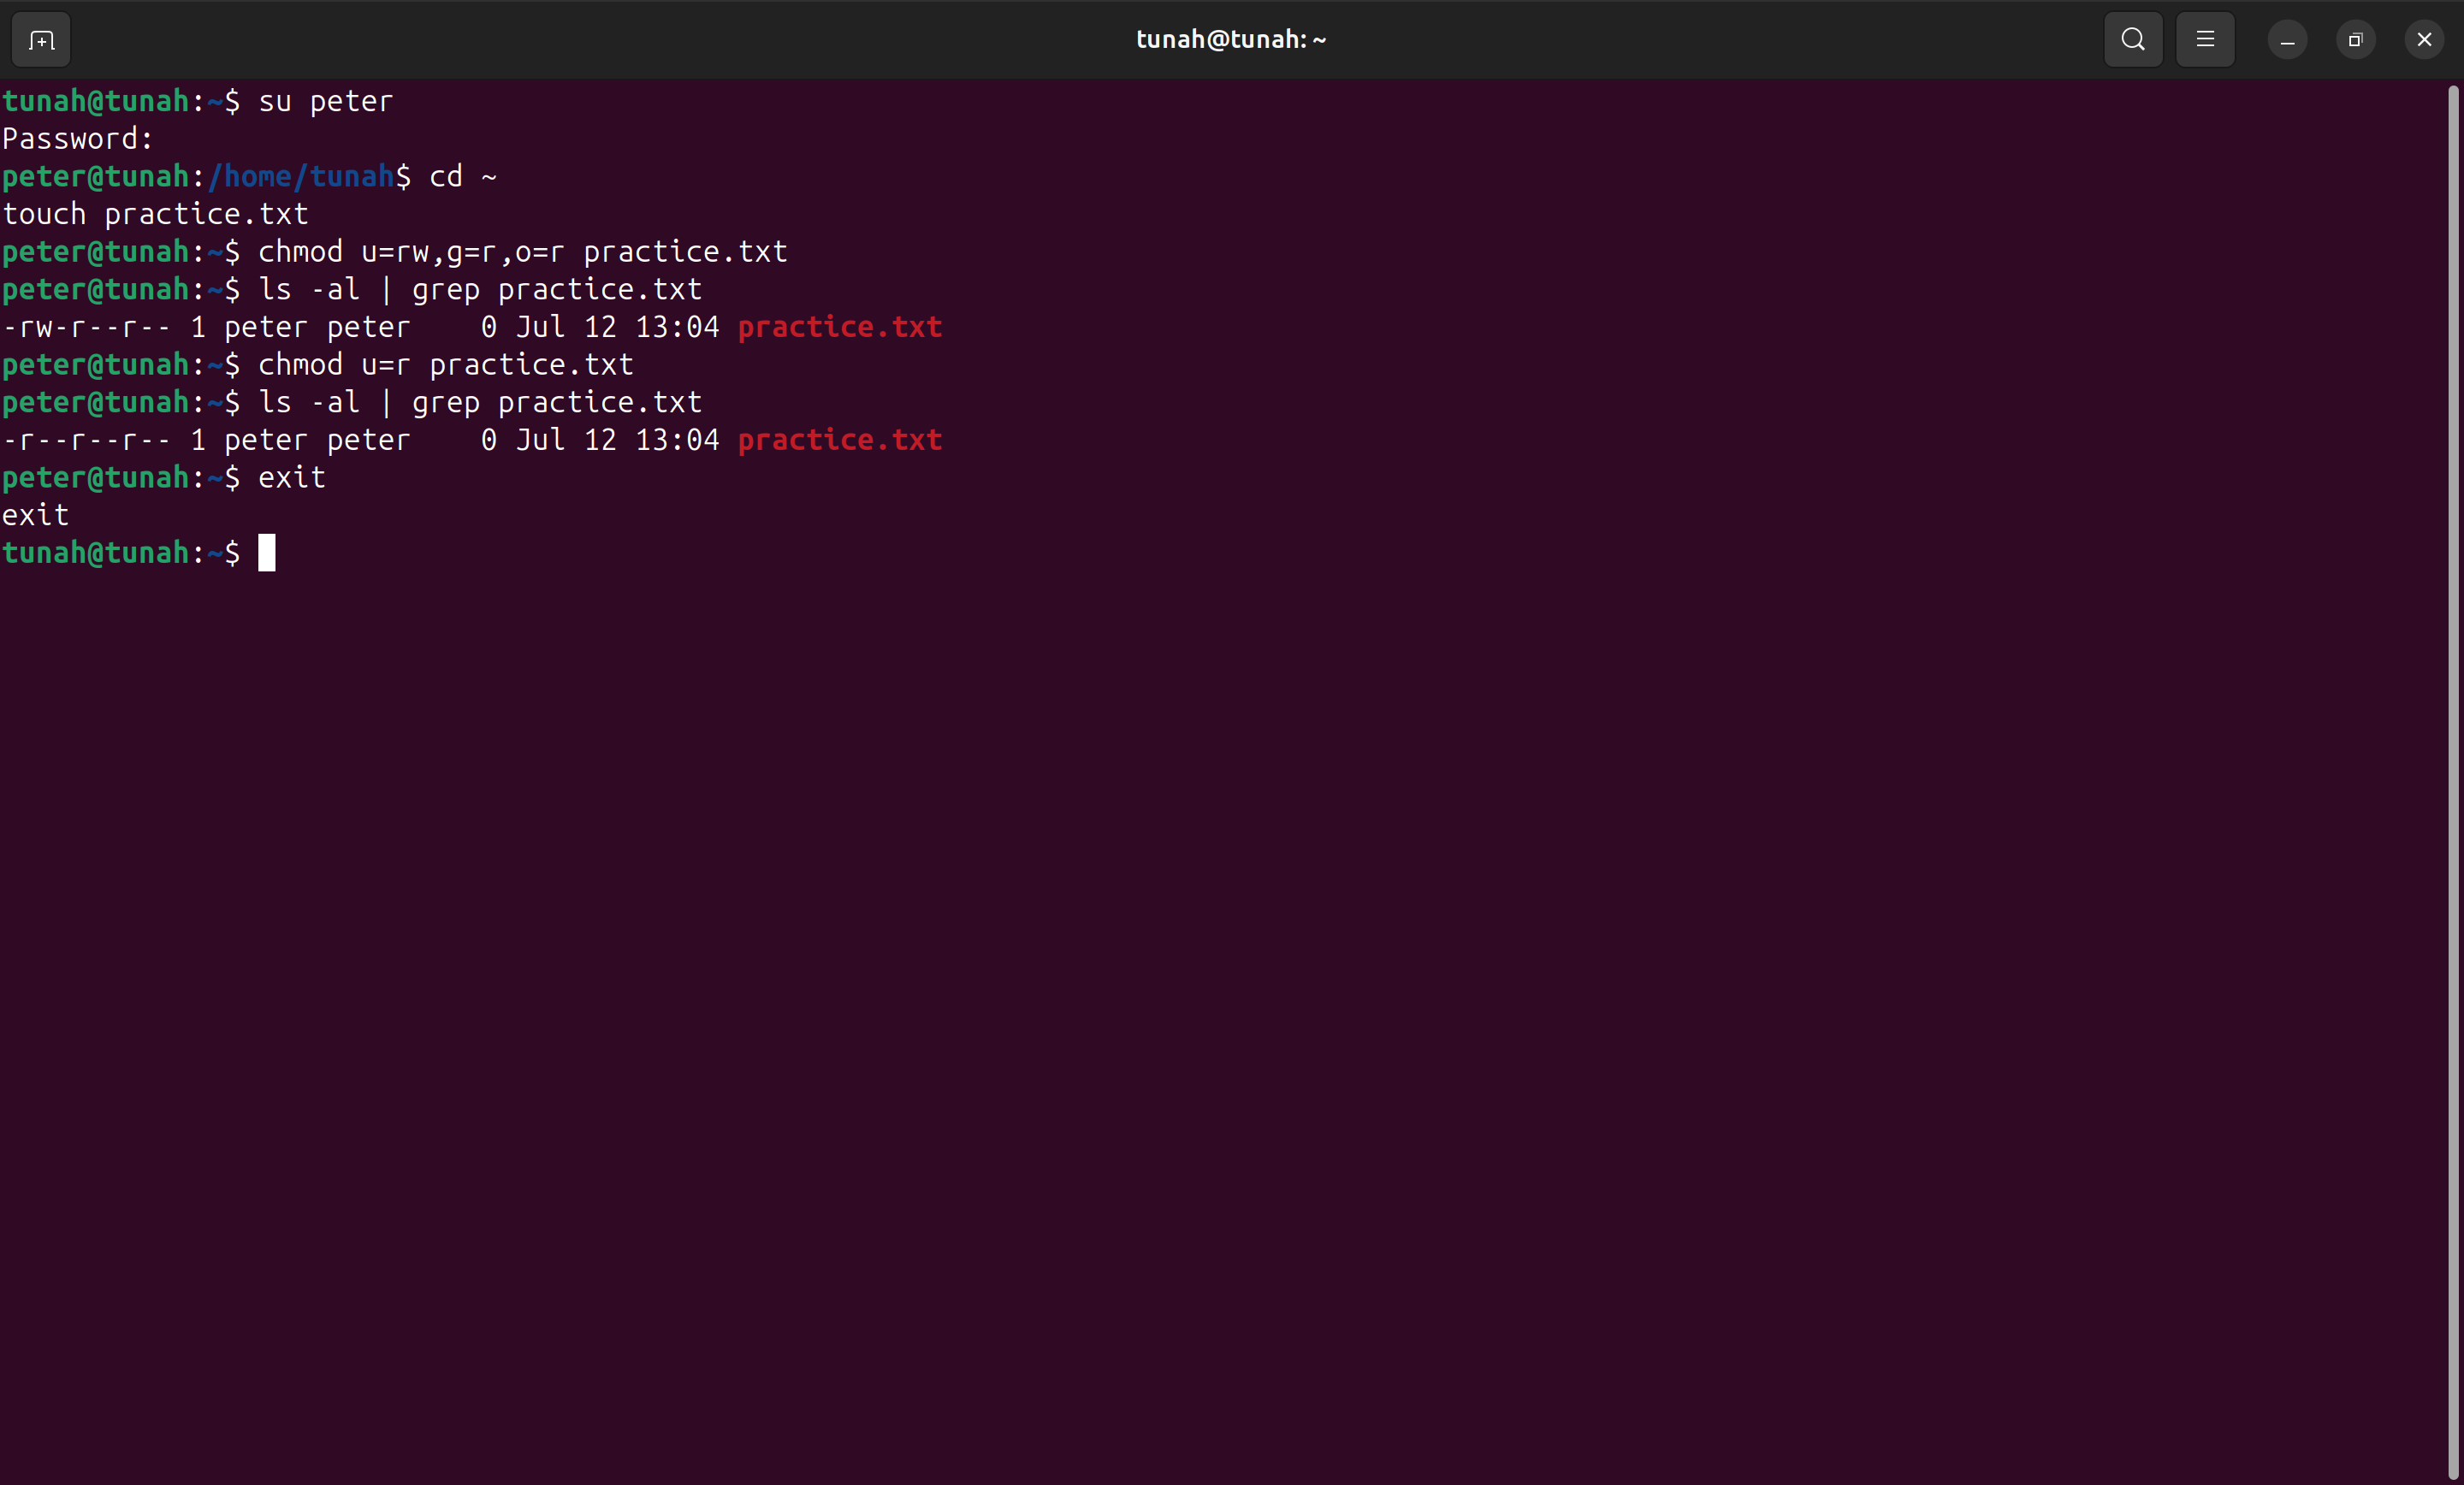
\includegraphics[width=\textwidth]{02/hello-sh-content.png}
        \caption{Nội dung script}
    \end{subfigure}
    \hfill
    \begin{subfigure}[b]{0.48\textwidth}
        \centering
        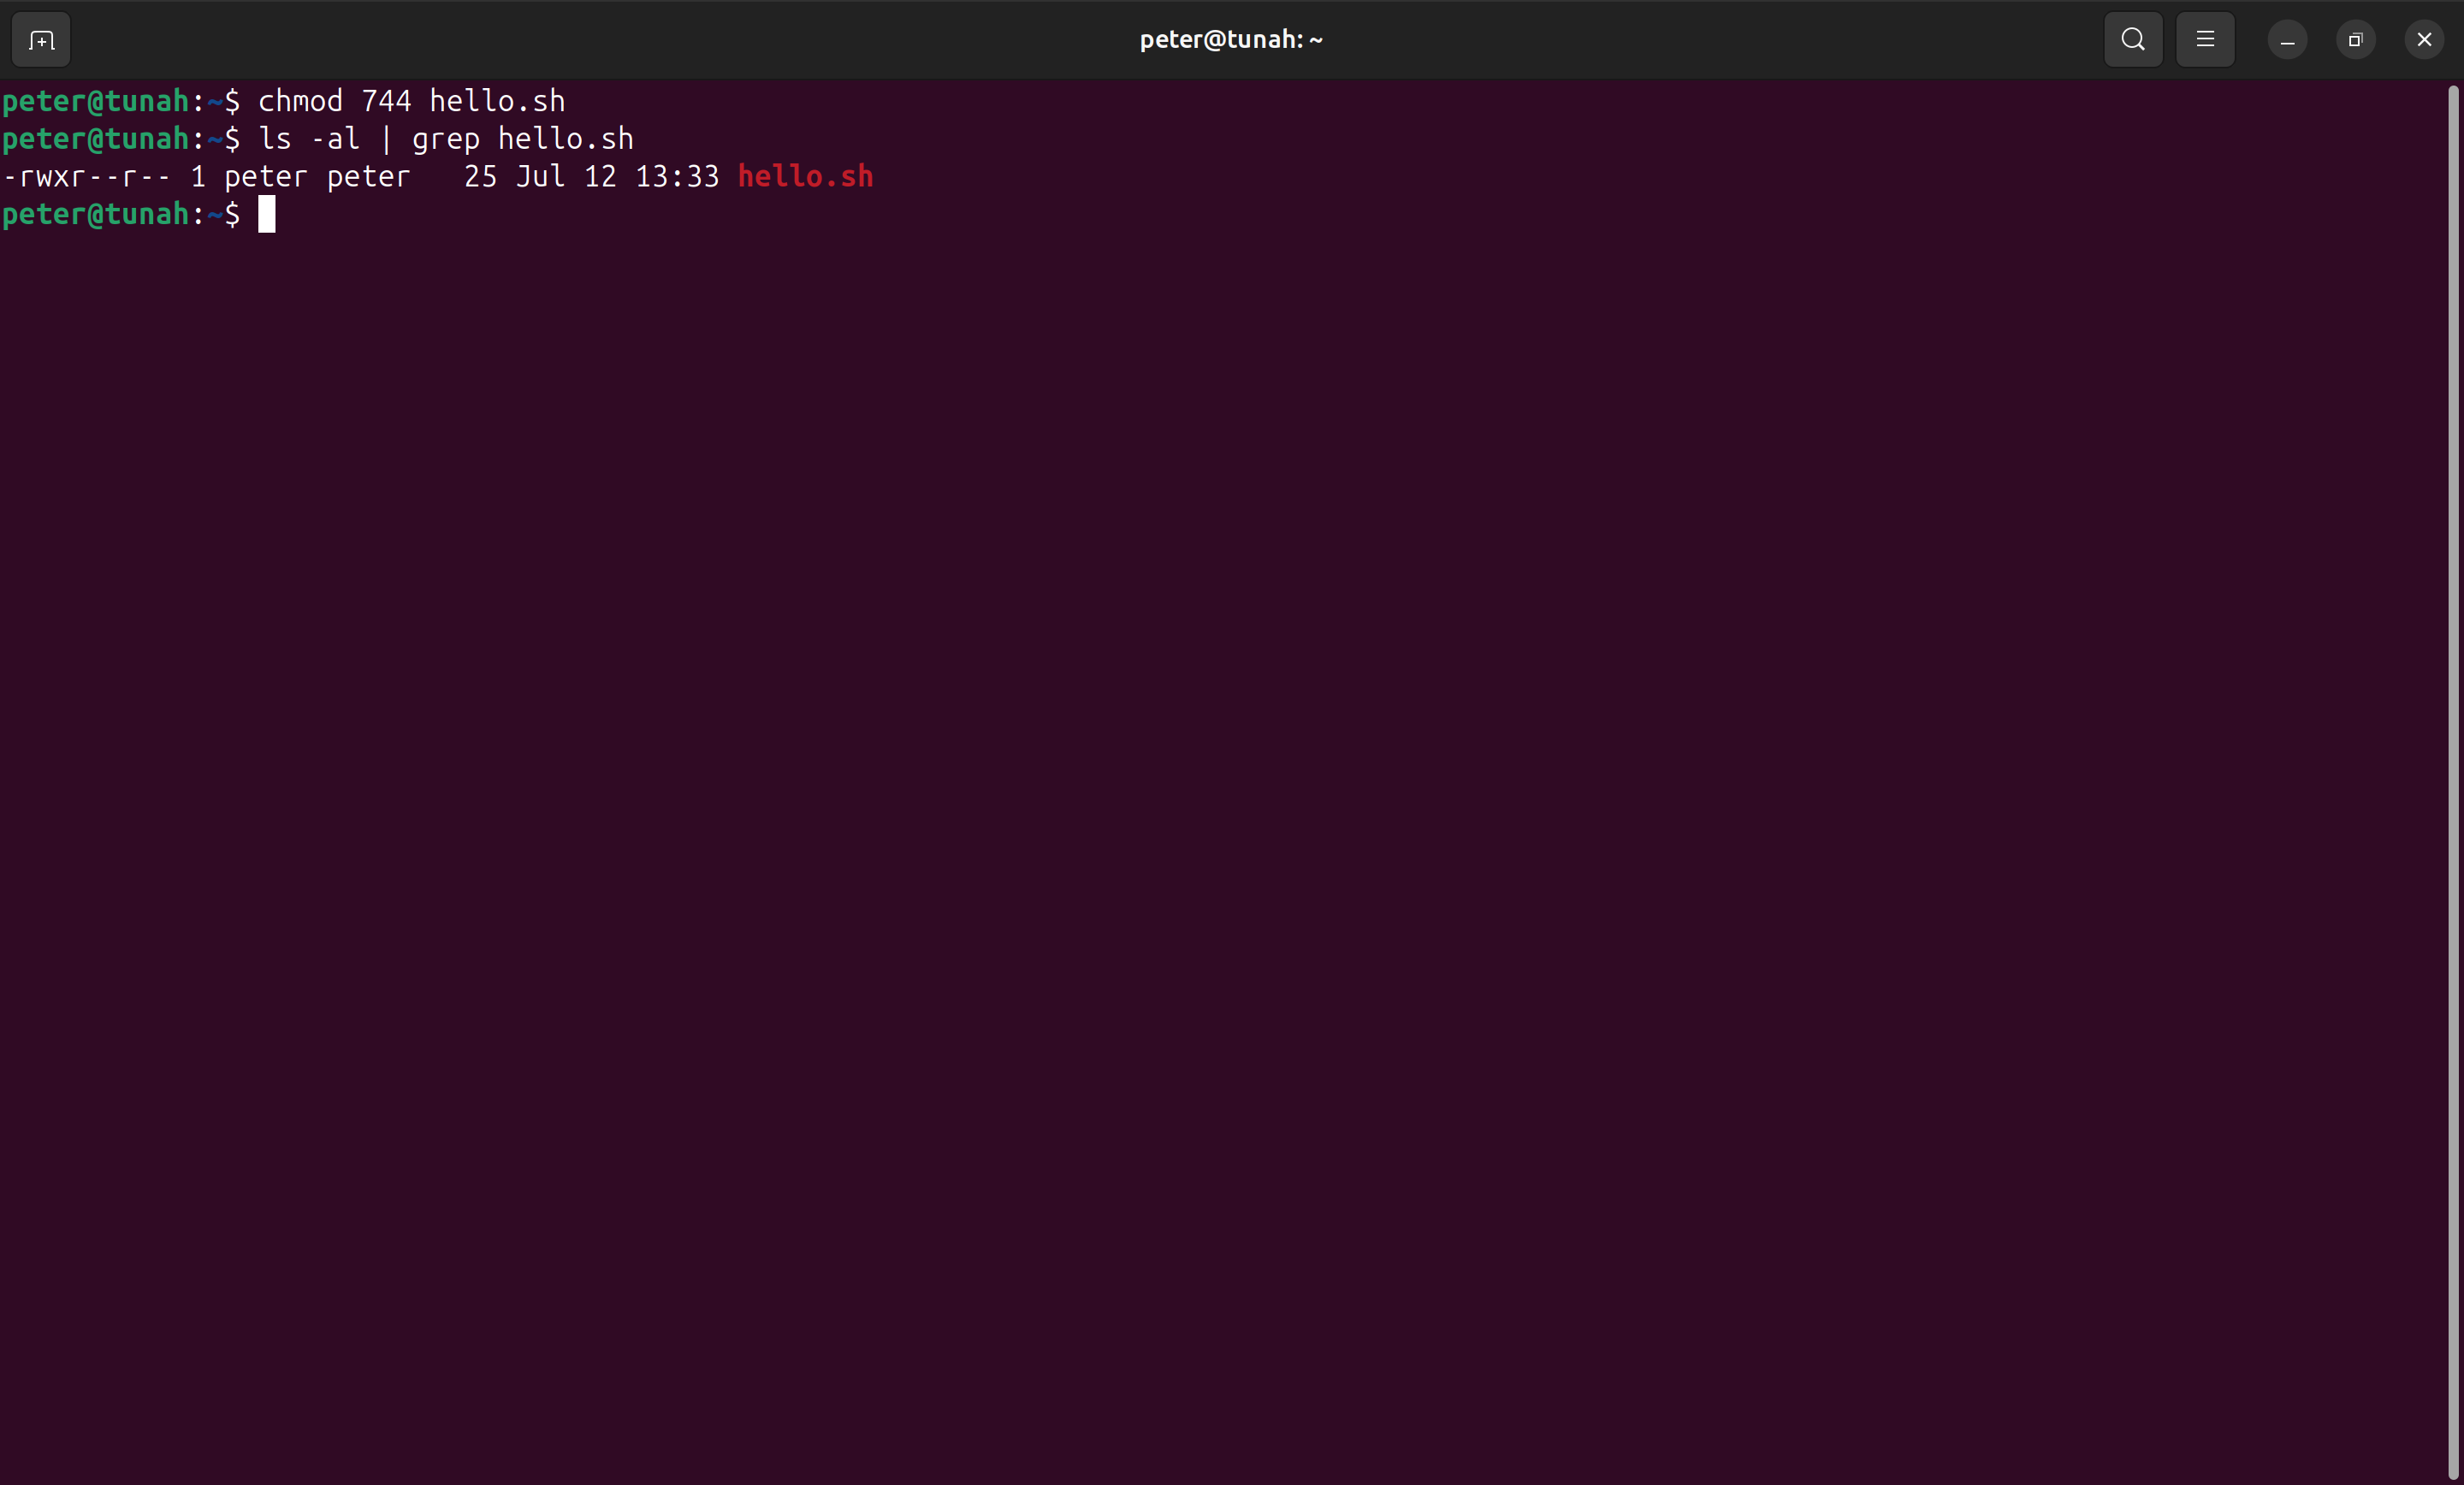
\includegraphics[width=\textwidth]{02/hello-sh-permission-744.png}
        \caption{Kiểm tra quyền 744}
    \end{subfigure}
    
    \vspace{0.5cm}
    \begin{subfigure}[b]{0.48\textwidth}
        \centering
        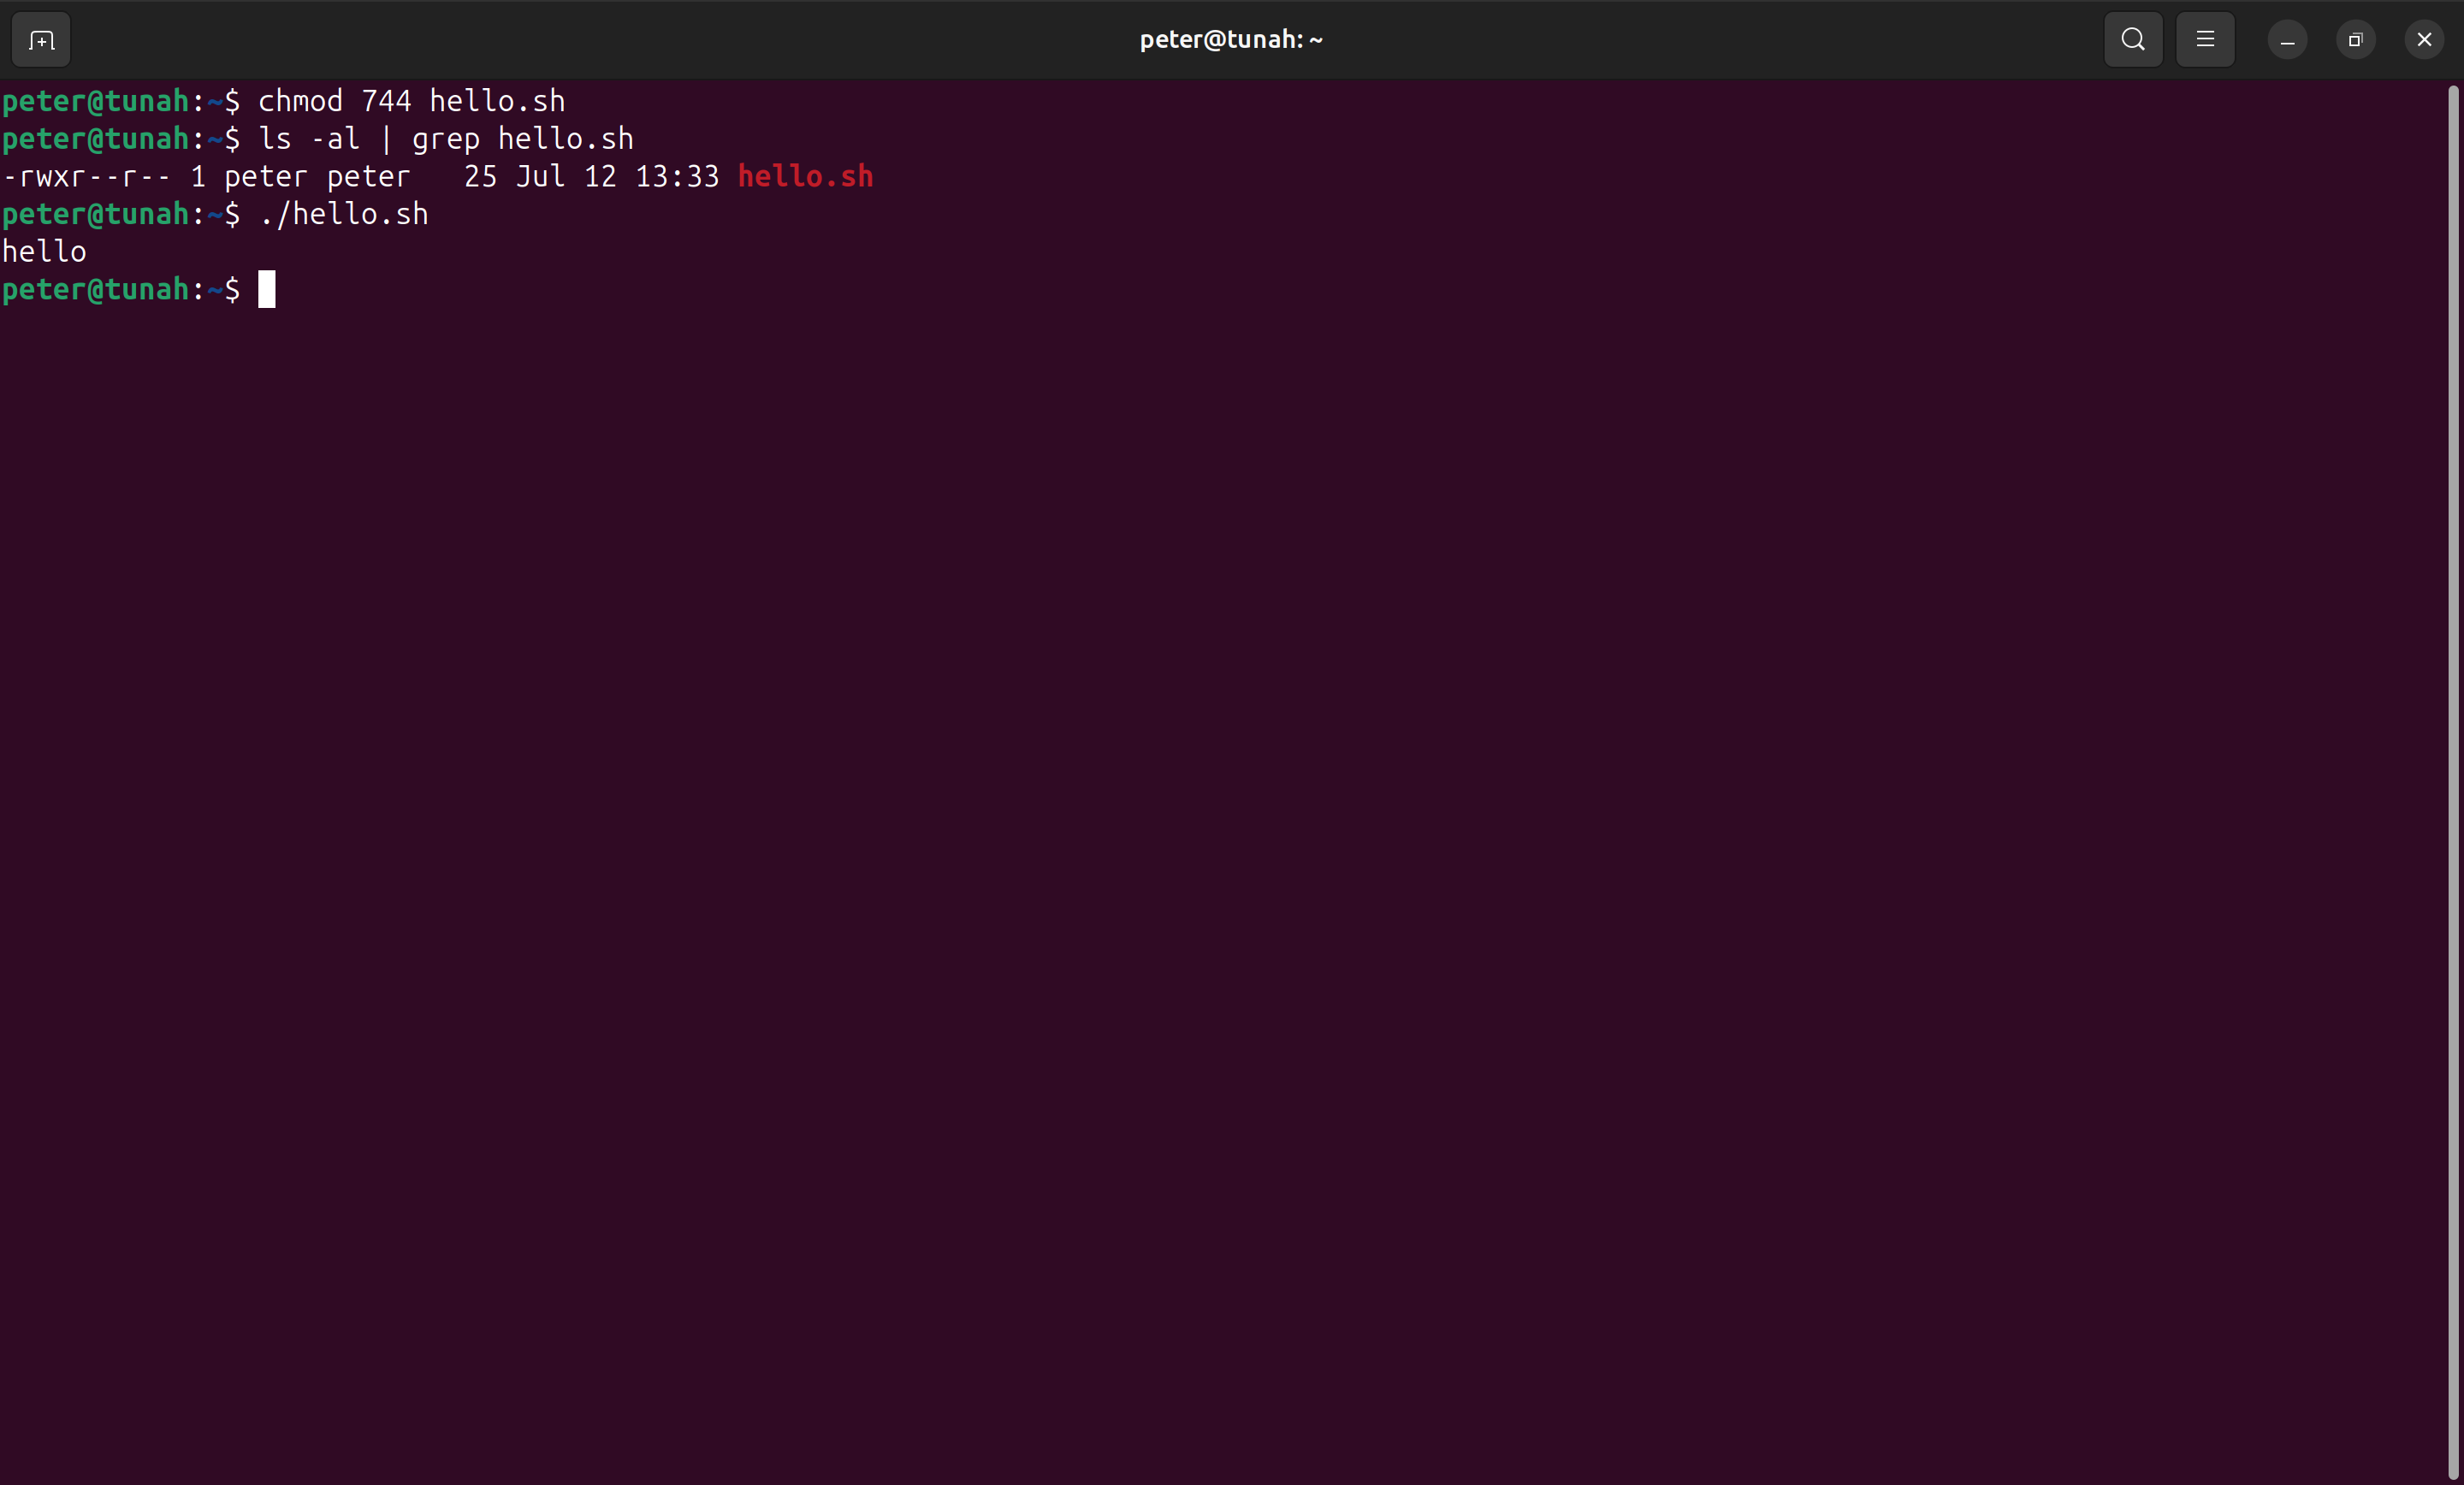
\includegraphics[width=\textwidth]{02/hello-sh-executed.png}
        \caption{Kết quả thực thi}
    \end{subfigure}
    \caption{Kết quả Bài tập 2: Numeric mode}
\end{figure}

\section{Quản lý Xuất Nhập File (File IO)}

\subsection{Tạo, Xem và Thêm nội dung vào File}

\textbf{Cách thực hiện:}
Sử dụng toán tử redirect (\texttt{>}) để tạo file \texttt{myfile.txt} chứa nội dung "Hello, Linux!" và xem nội dung bằng \texttt{cat}. Tiếp tục dùng toán tử append (\texttt{>>}) để thêm dòng mới mà không làm mất dữ liệu cũ.

\begin{lstlisting}[language=bash]
# Tao file va xem
echo "Hello, Linux!" > myfile.txt
cat myfile.txt

# Them noi dung va xem lai
echo "Welcome to Linux file management." >> myfile.txt
cat myfile.txt
\end{lstlisting}

\textbf{Kết quả:}
Tập tin được tạo và thêm nội dung thành công, các toán tử redirect hoạt động đúng như lý thuyết.

\begin{figure}[H]
    \centering
    \begin{subfigure}[b]{0.45\textwidth}
        \centering
        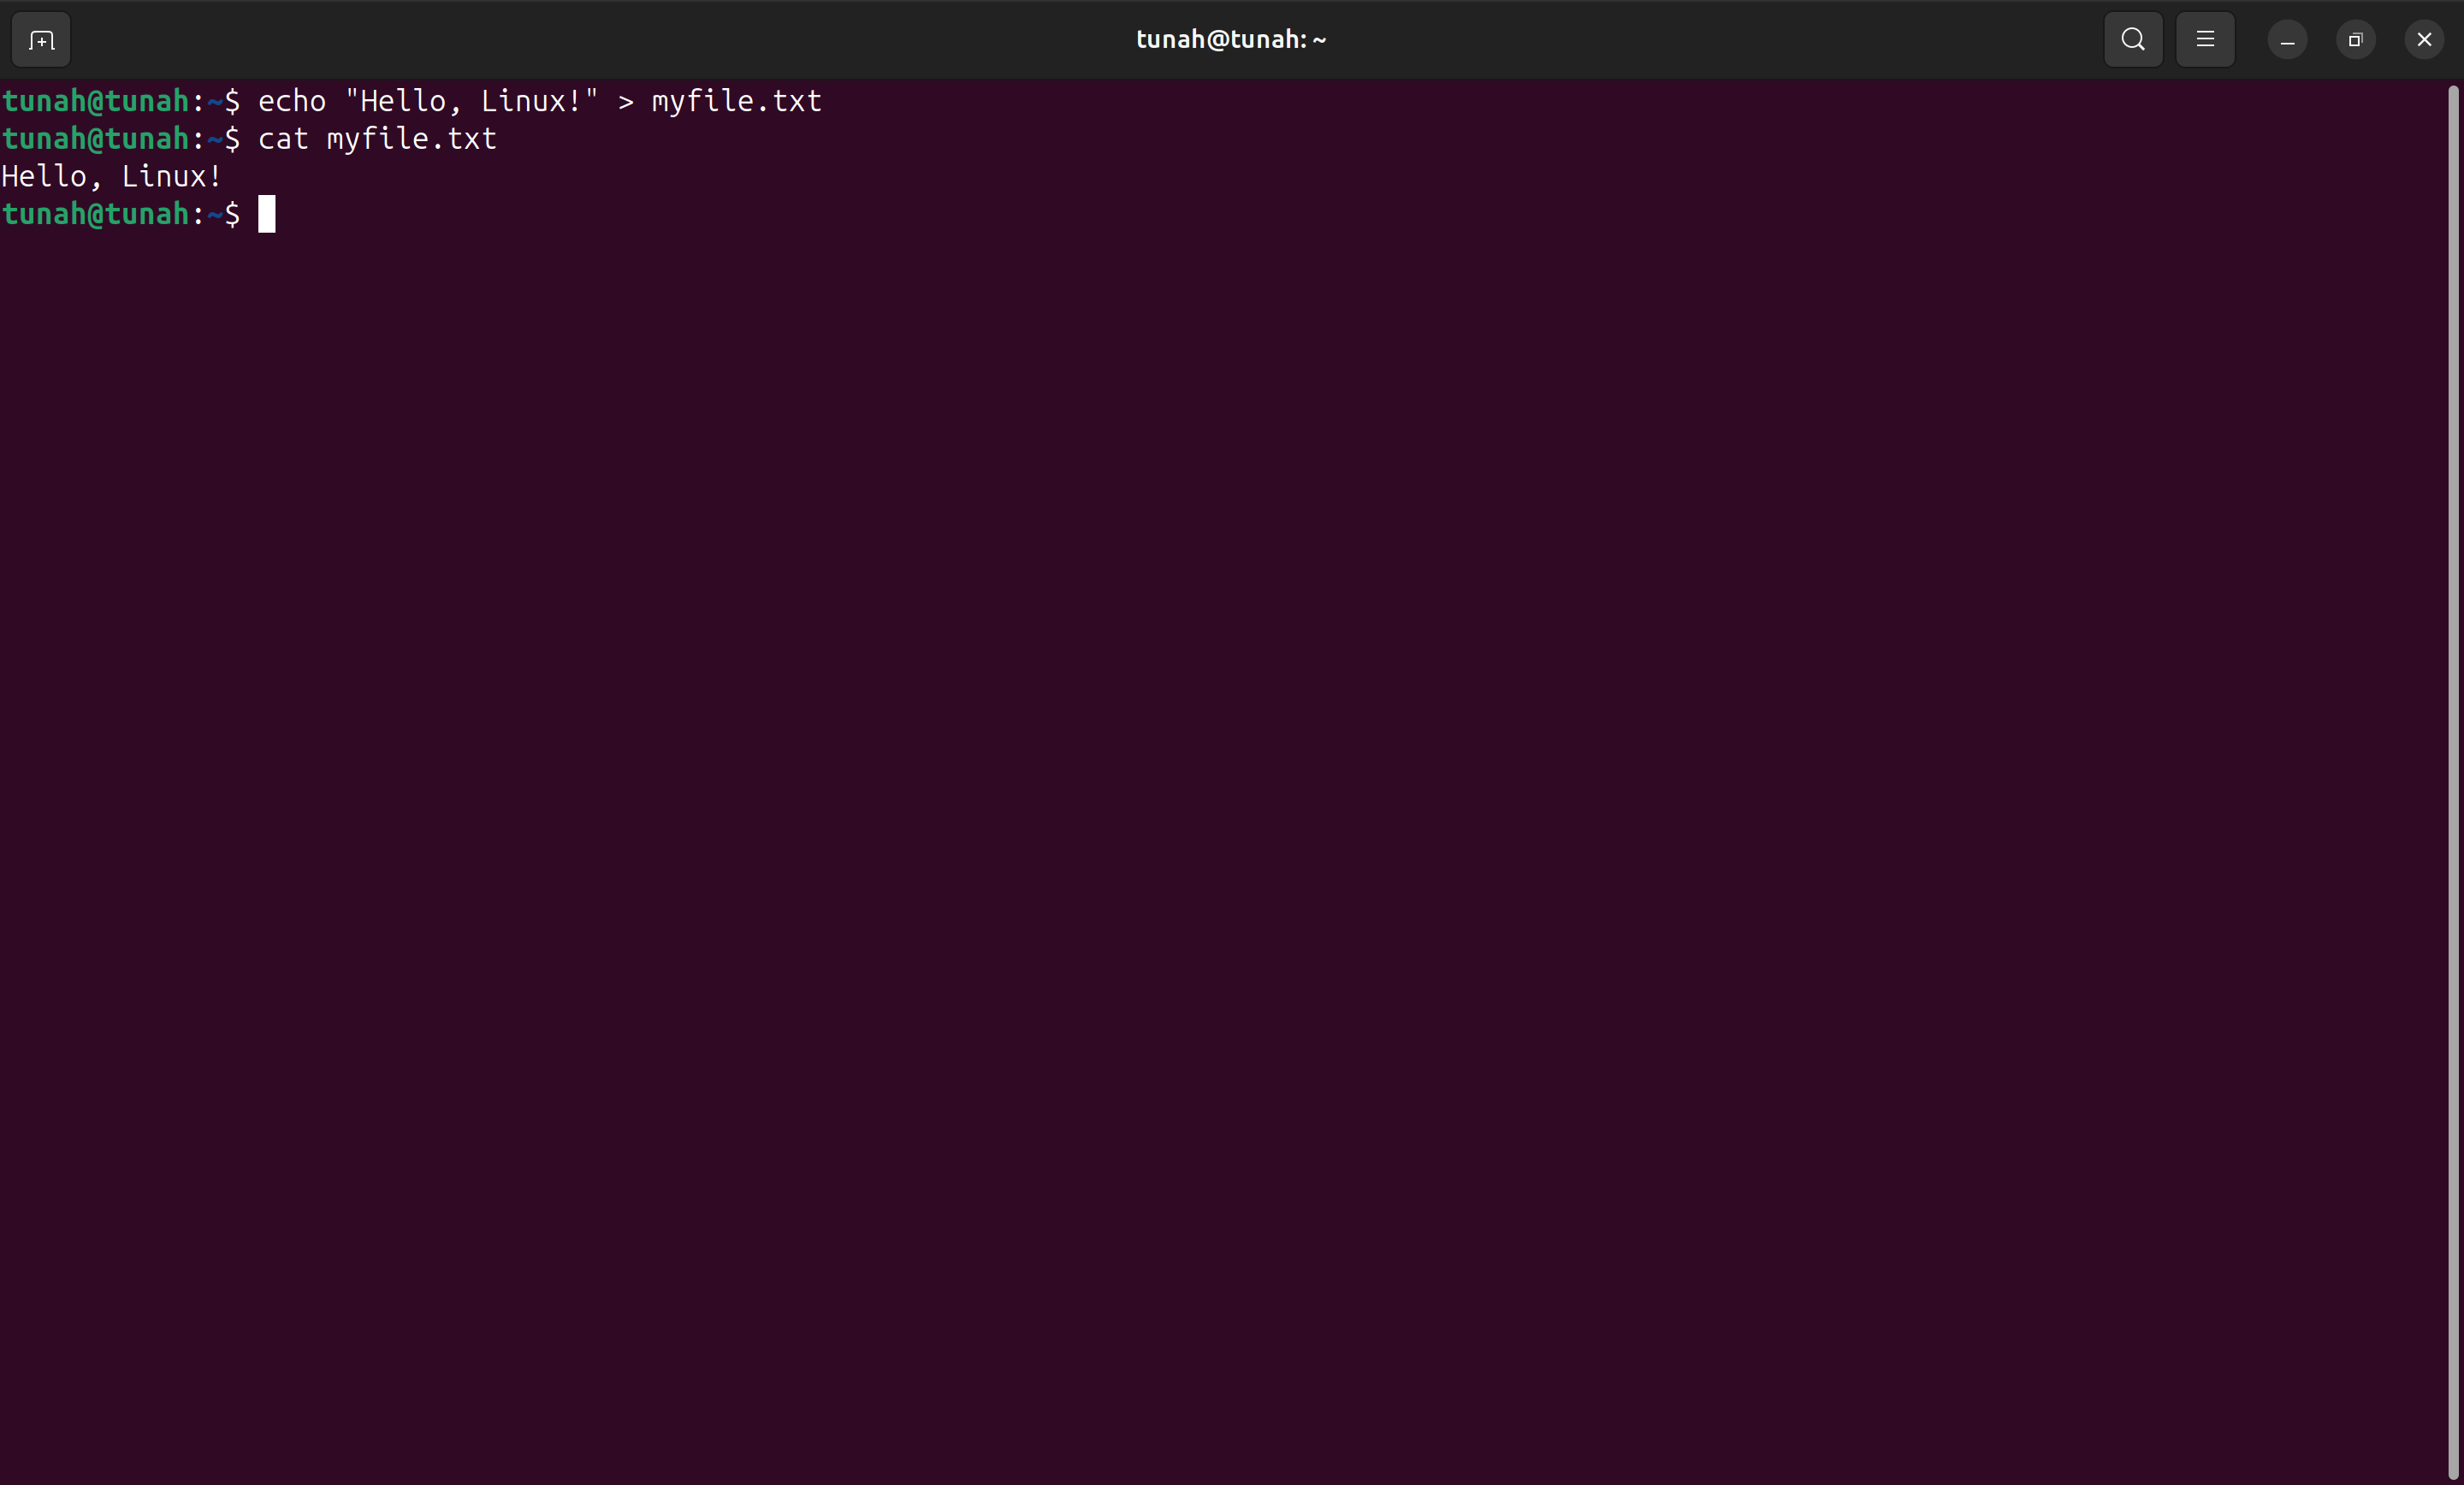
\includegraphics[width=\textwidth]{03/create-myfile.png}
        \caption{Tạo file myfile.txt}
    \end{subfigure}
    \hfill
    \begin{subfigure}[b]{0.45\textwidth}
        \centering
        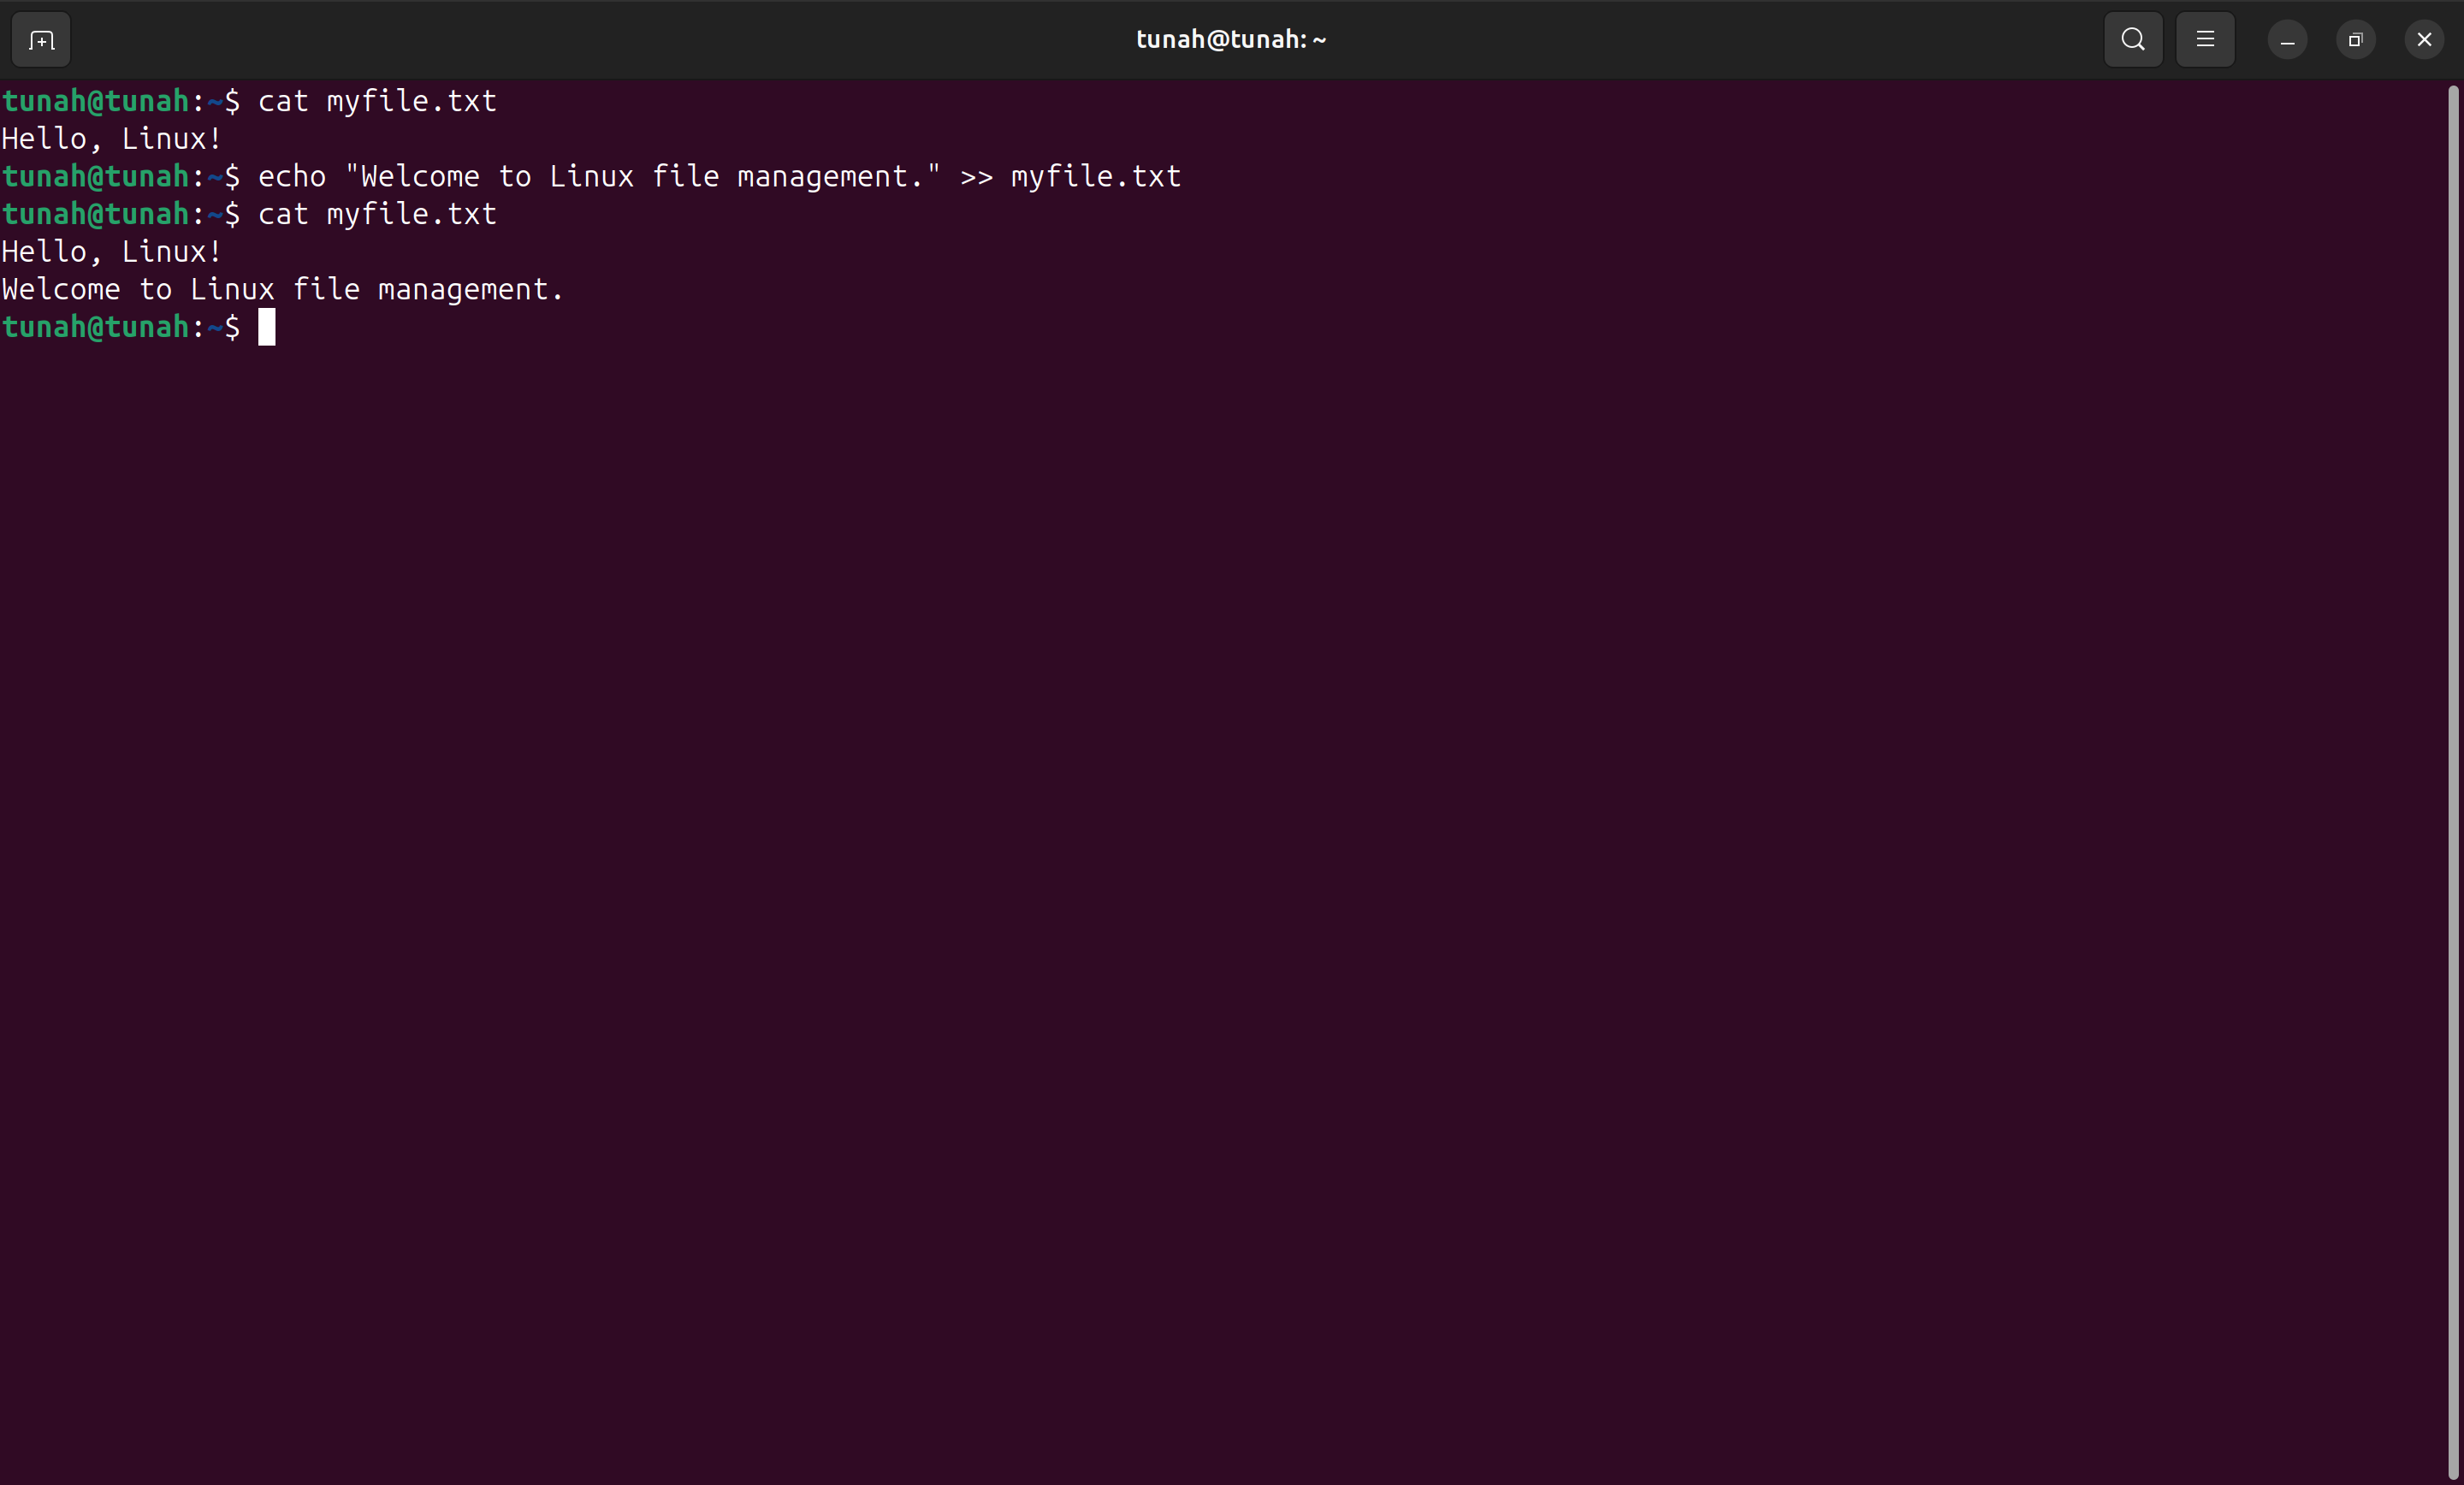
\includegraphics[width=\textwidth]{03/append-myfile.png}
        \caption{Thêm nội dung (Append)}
    \end{subfigure}
    \caption{Thao tác cơ bản với File}
\end{figure}

\subsection{Đếm số dòng và từ}

\textbf{Cách thực hiện:}
Sử dụng lệnh \texttt{wc} (word count) với tùy chọn \texttt{-l} để đếm số dòng và \texttt{-w} để đếm số từ trong tập tin \texttt{myfile.txt}.

\begin{lstlisting}[language=bash]
wc -l myfile.txt
wc -w myfile.txt
\end{lstlisting}

\textbf{Kết quả:}
Hệ thống đếm chính xác số lượng dòng (2 dòng) và số lượng từ.

\begin{figure}[H]
    \centering
    \begin{subfigure}[b]{0.45\textwidth}
        \centering
        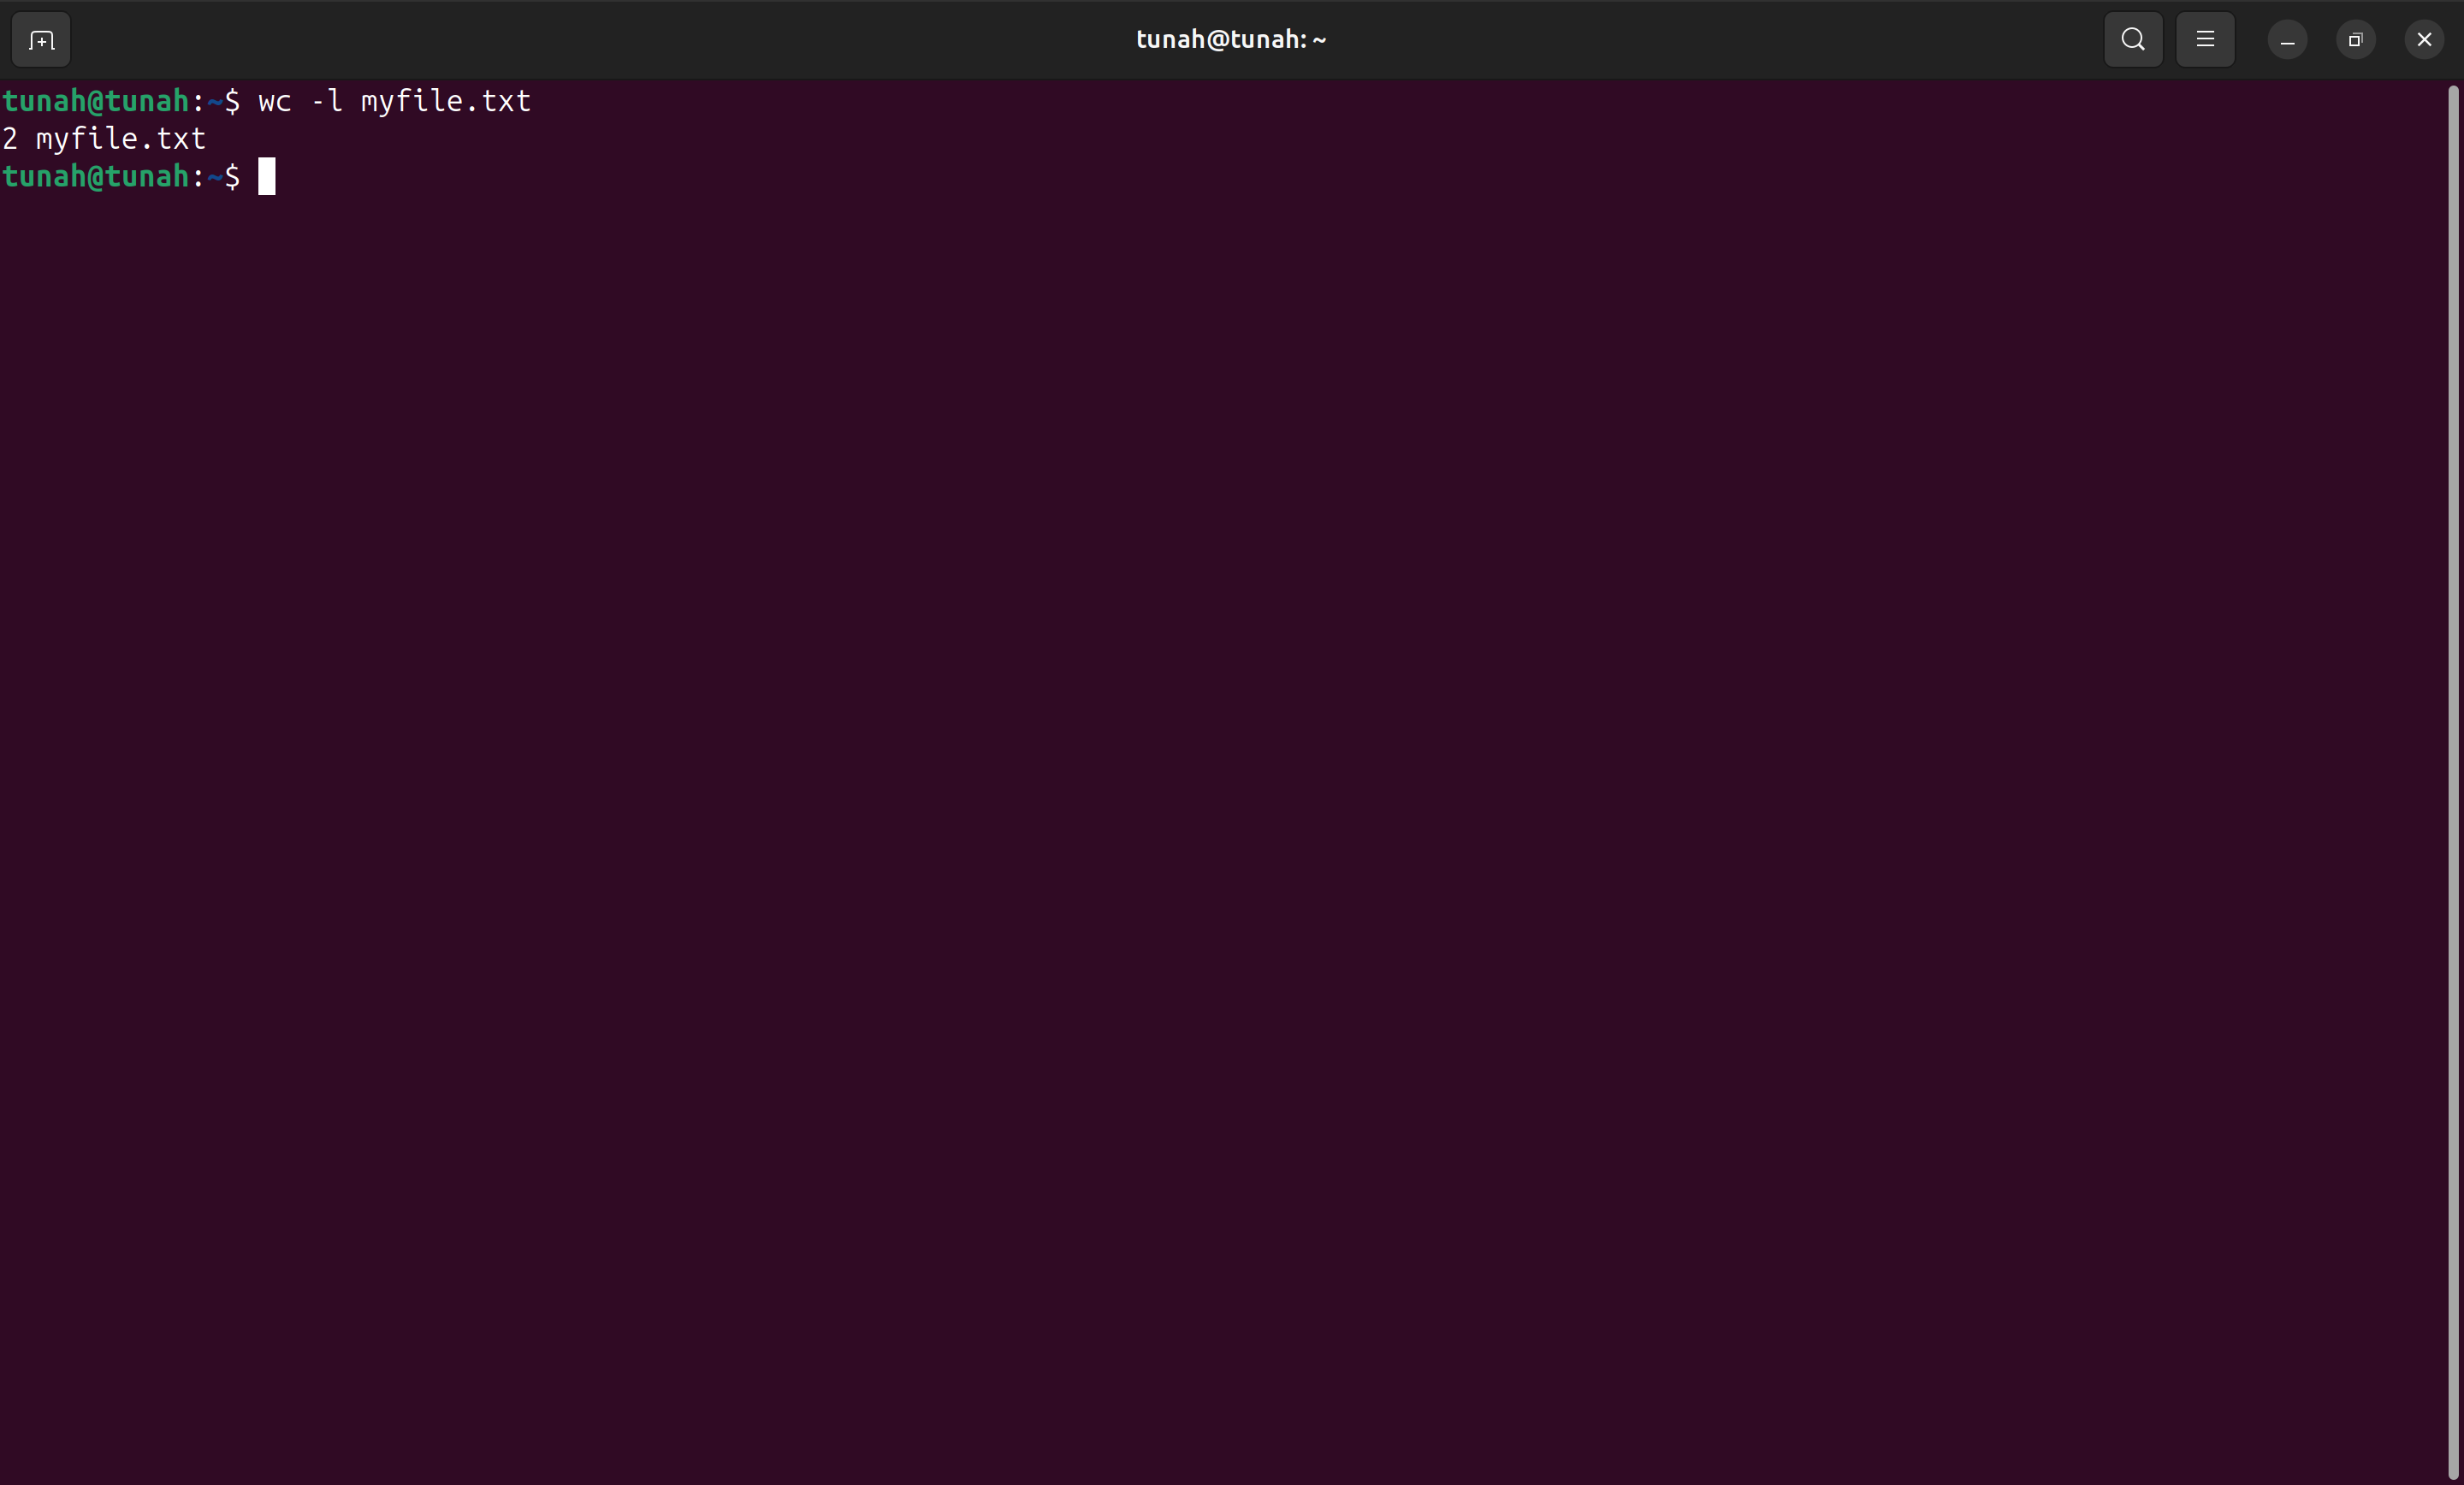
\includegraphics[width=\textwidth]{03/wc-lines.png}
        \caption{Đếm số dòng}
    \end{subfigure}
    \hfill
    \begin{subfigure}[b]{0.45\textwidth}
        \centering
        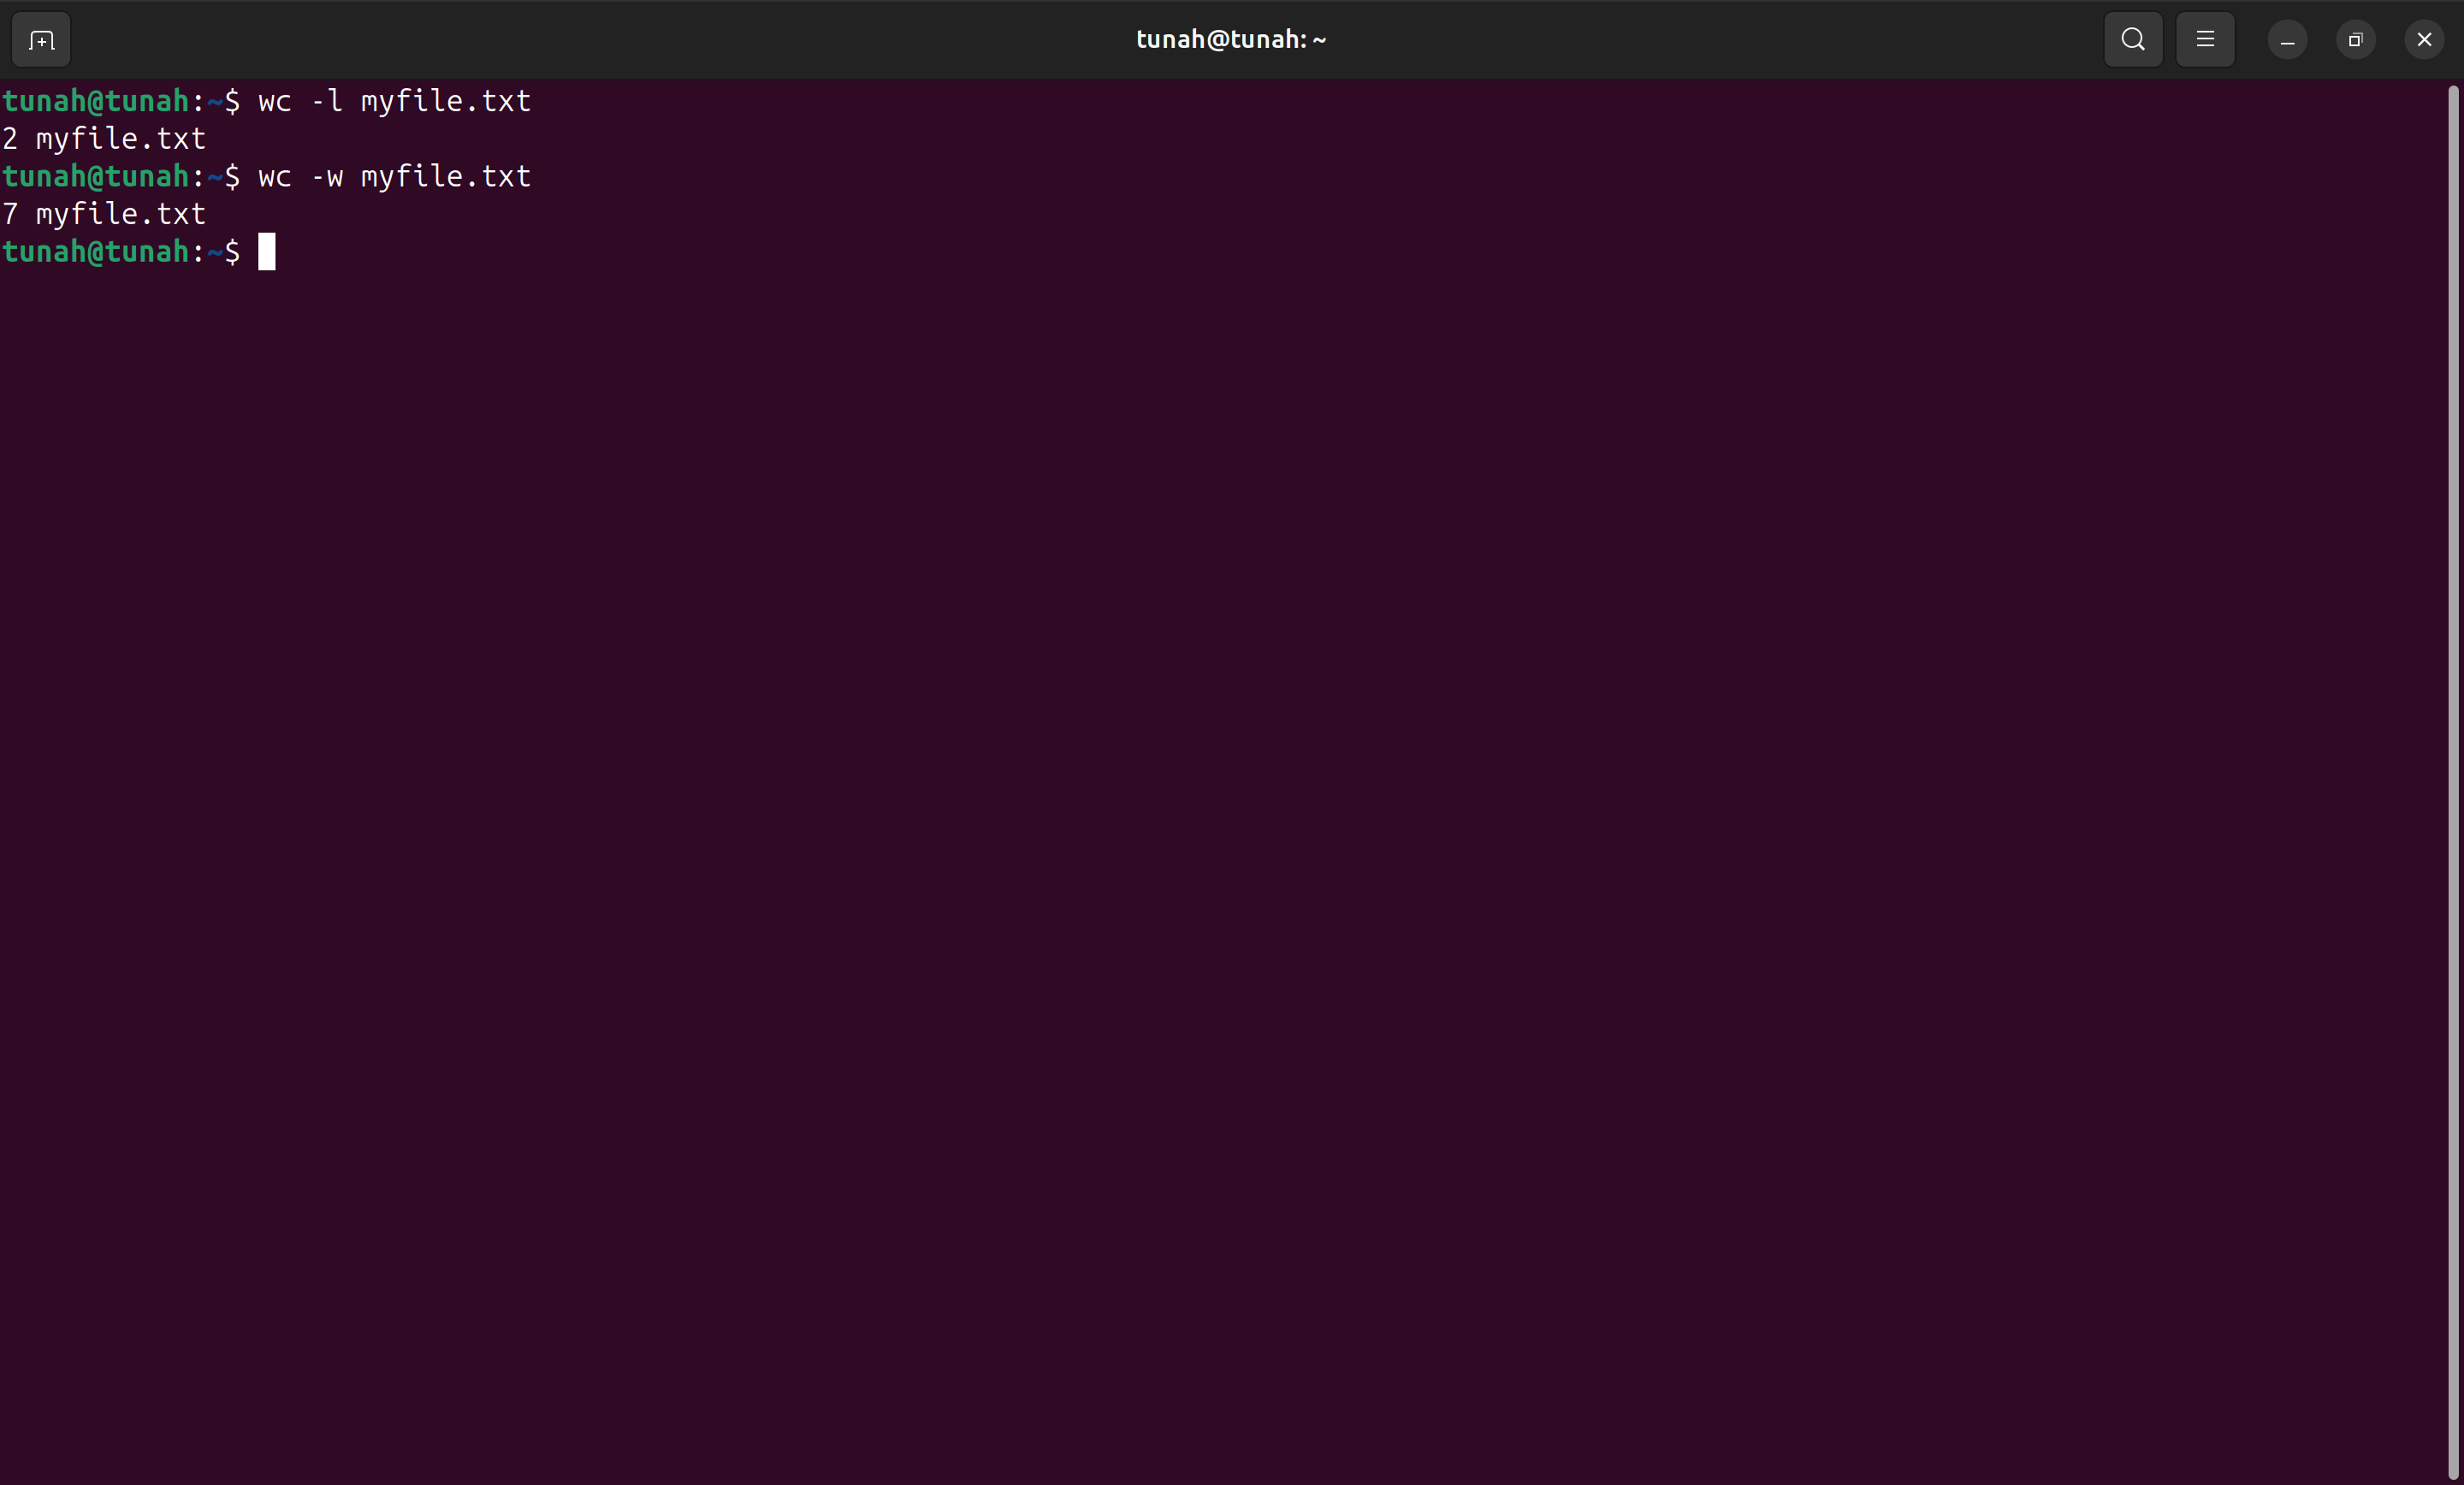
\includegraphics[width=\textwidth]{03/wc-words.png}
        \caption{Đếm số từ}
    \end{subfigure}
    \caption{Lệnh đếm dòng và từ}
\end{figure}

\subsection{Sao chép, Di chuyển và Xóa File}

\textbf{Cách thực hiện:}
Tiến hành sao chép \texttt{myfile.txt} thành \texttt{myfile\_backup.txt}, sau đó di chuyển bản backup vào thư mục \texttt{/tmp/}. Cuối cùng, xóa bỏ file gốc \texttt{myfile.txt}.

\begin{lstlisting}[language=bash]
# Sao chep
cp myfile.txt myfile_backup.txt

# Di chuyen
mv myfile_backup.txt /tmp/

# Xoa file
rm myfile.txt
\end{lstlisting}

\textbf{Kết quả:}
Các lệnh thao tác tập tin hoạt động chính xác. File gốc được xóa và bản backup nằm an toàn trong \texttt{/tmp/}.

\begin{figure}[H]
    \centering
    \begin{subfigure}[b]{0.45\textwidth}
        \centering
        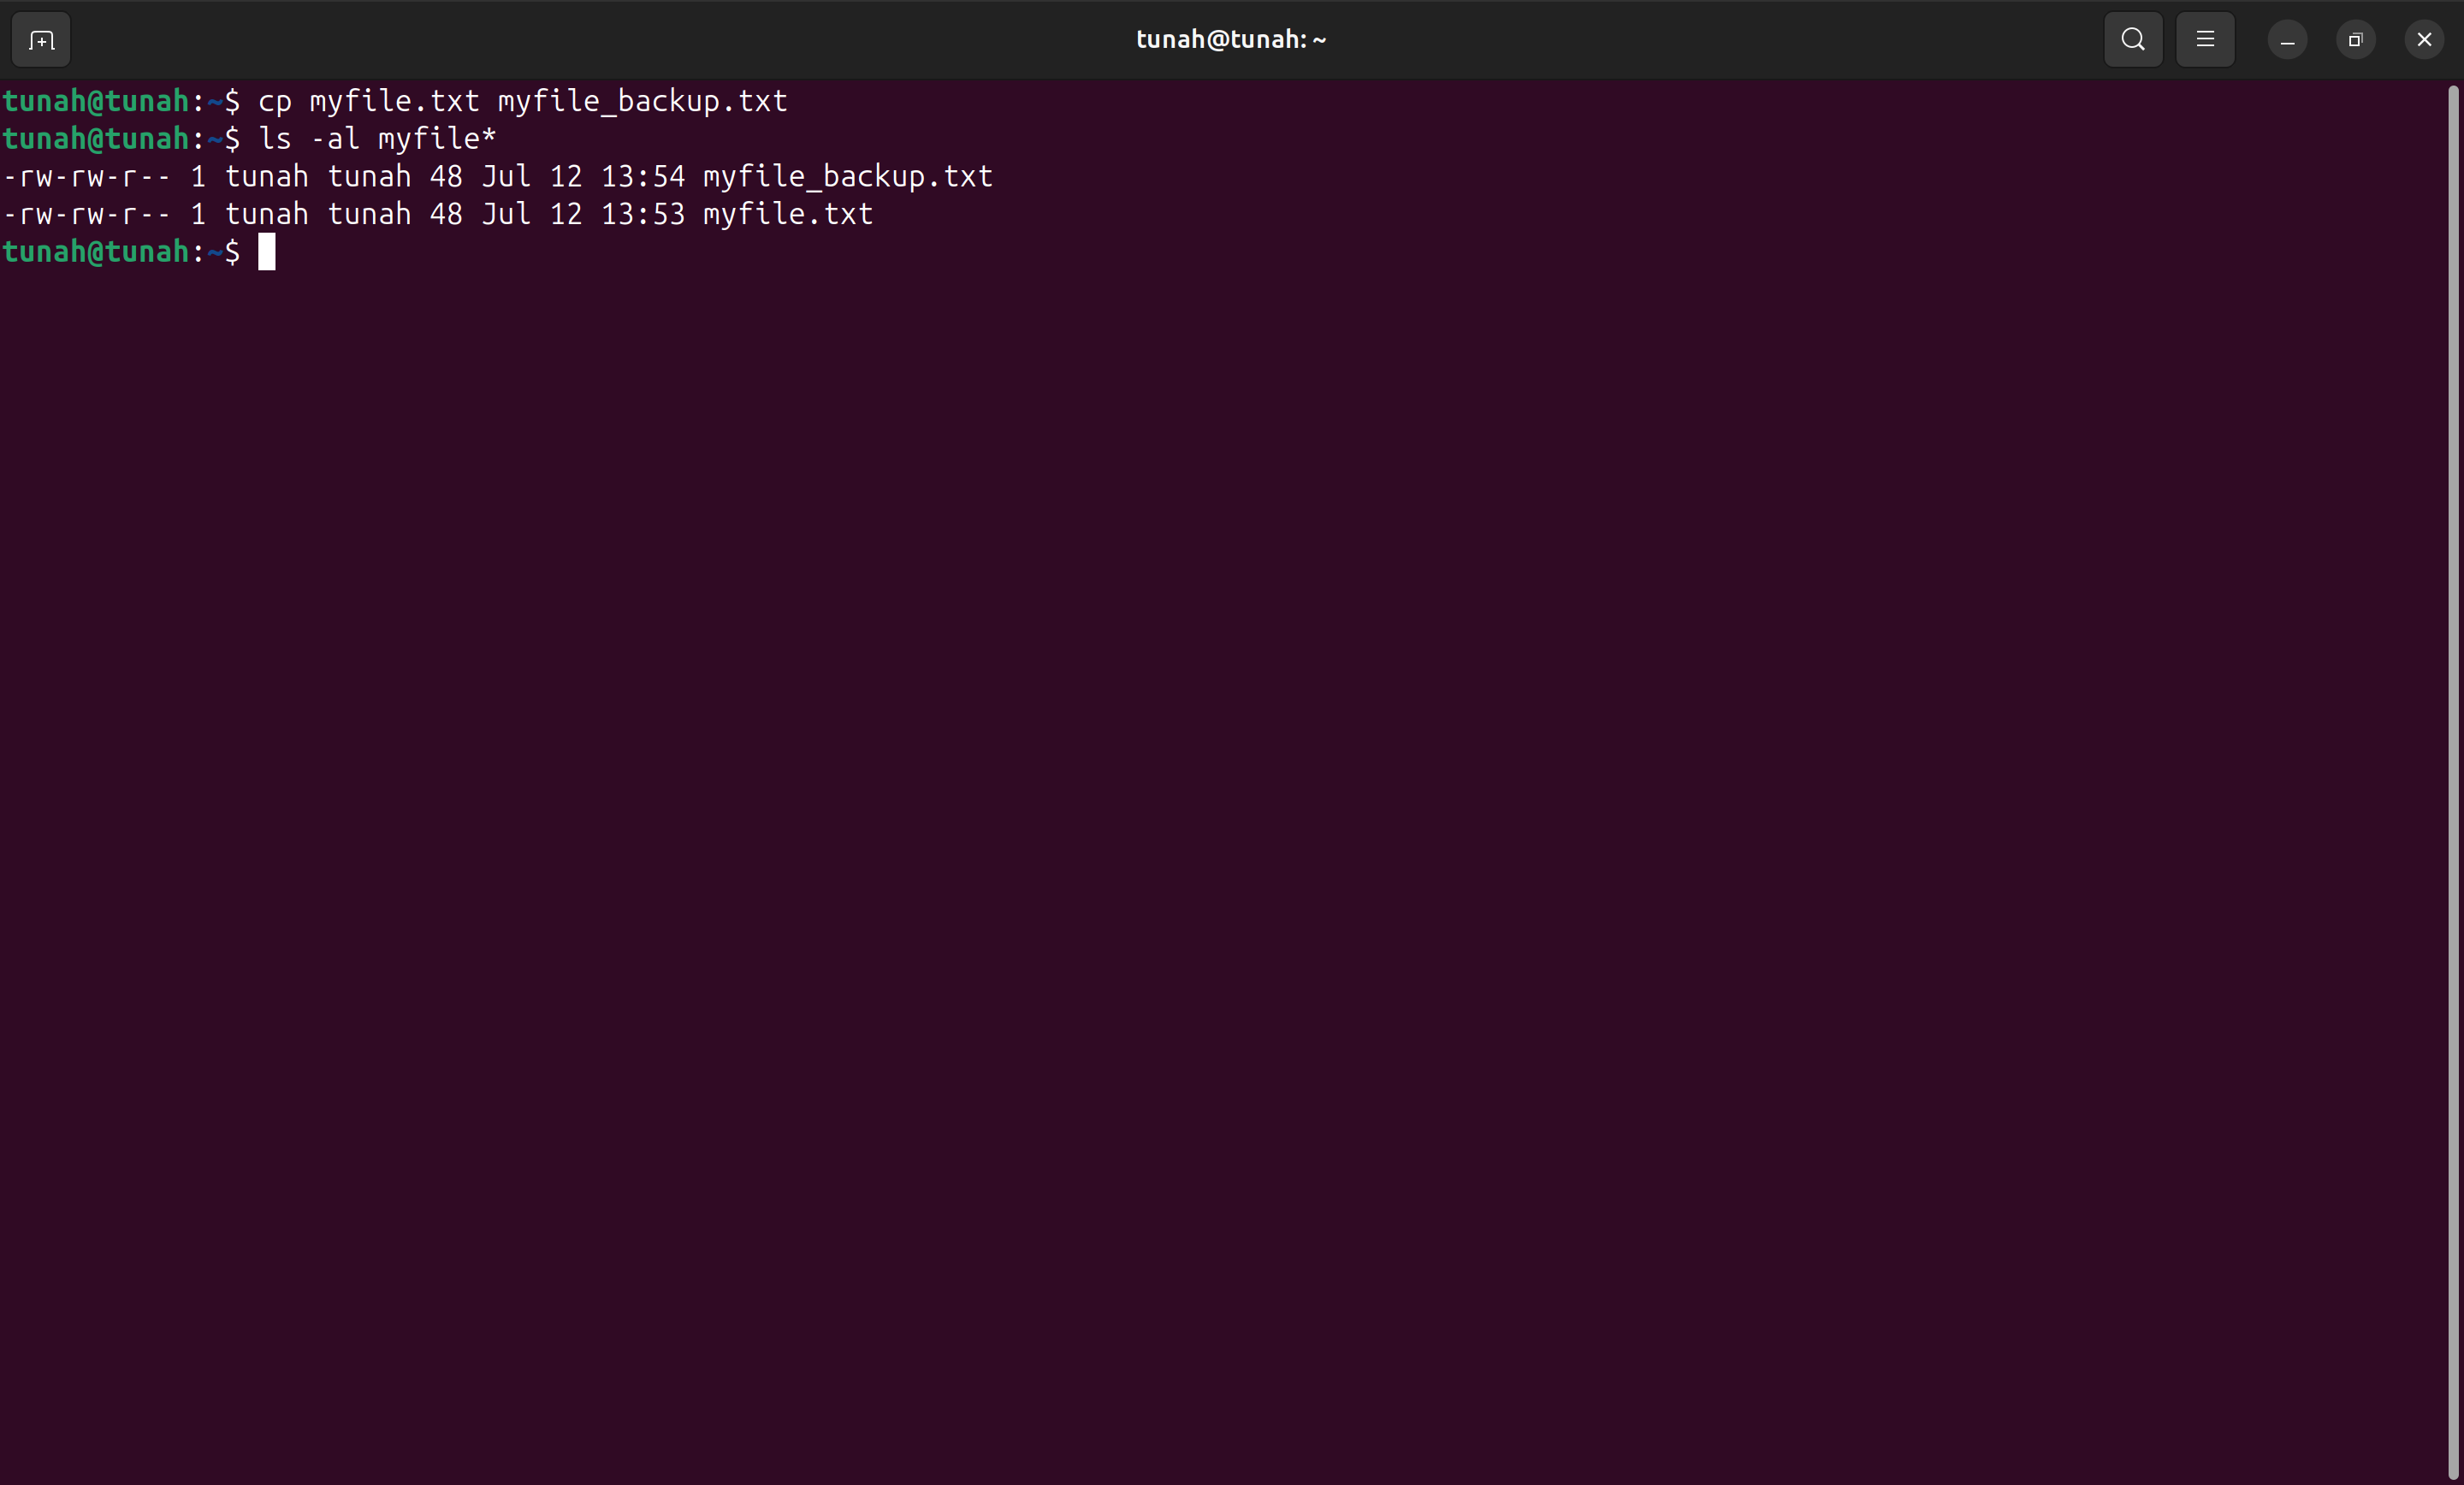
\includegraphics[width=\textwidth]{03/cp-myfile-backup.png}
        \caption{Sao chép file}
    \end{subfigure}
    \hfill
    \begin{subfigure}[b]{0.45\textwidth}
        \centering
        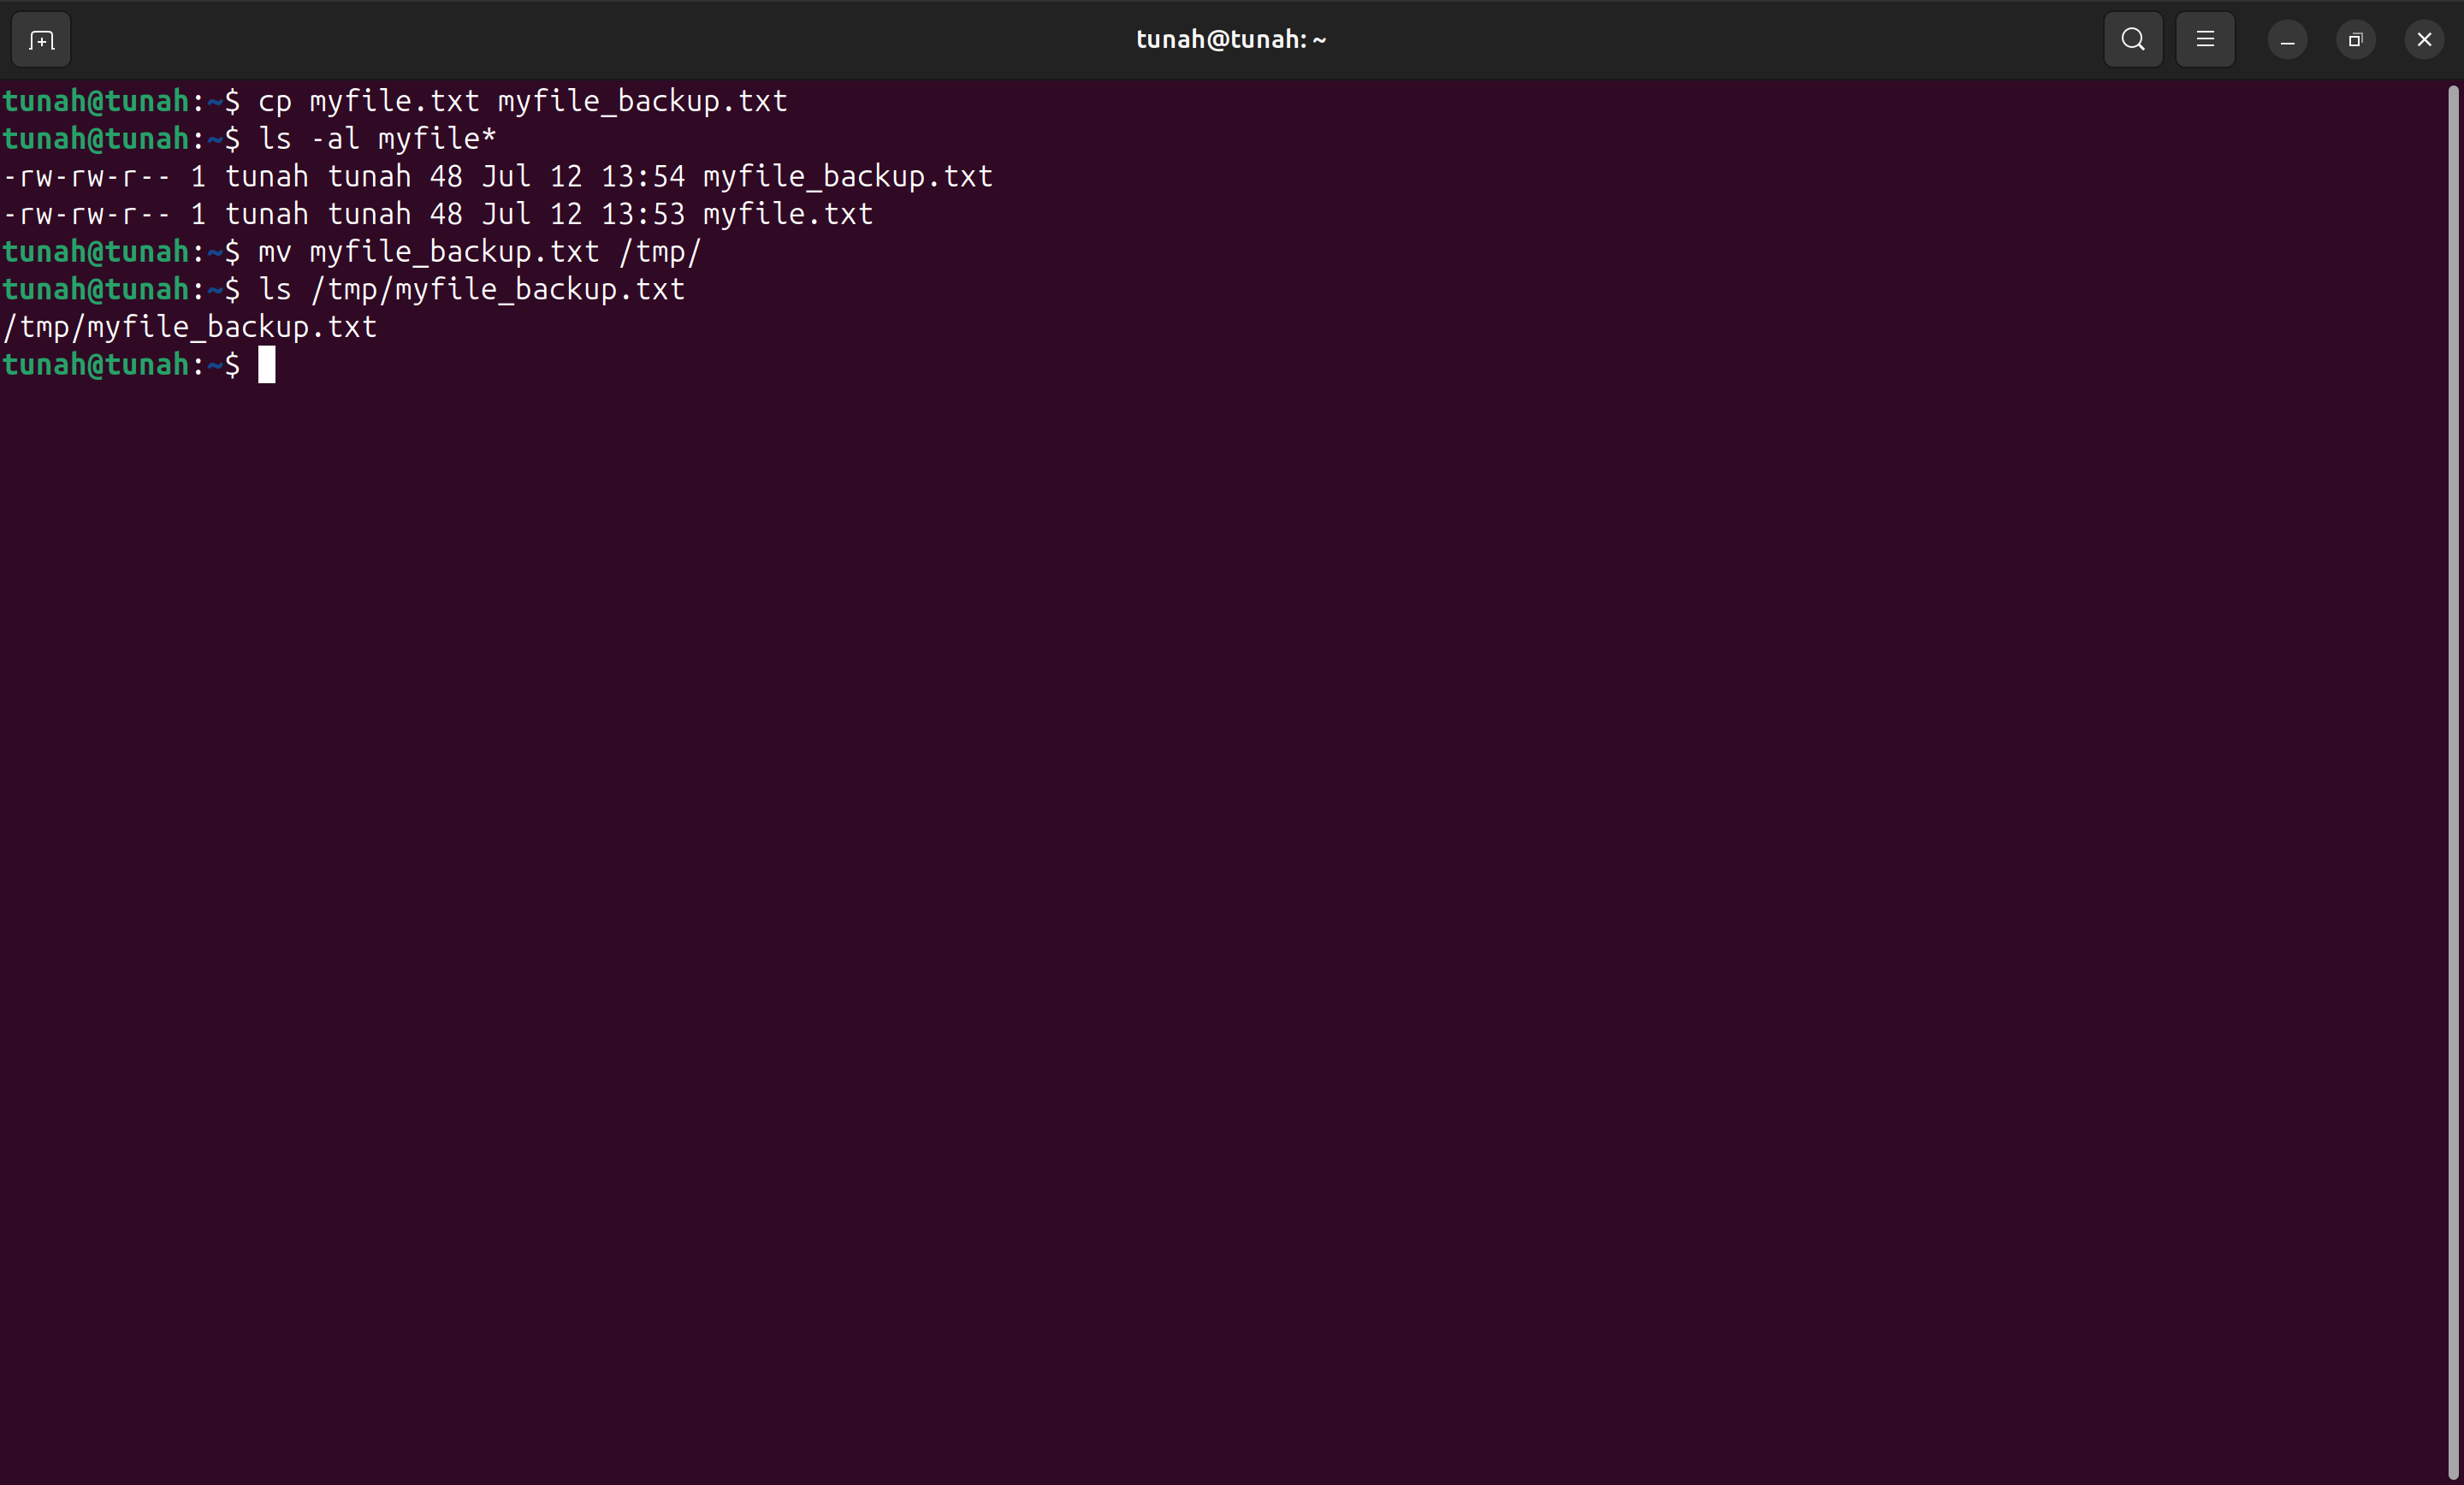
\includegraphics[width=\textwidth]{03/mv-to-tmp.png}
        \caption{Di chuyển file sang /tmp}
    \end{subfigure}
    
    \vspace{0.5cm}
    \begin{subfigure}[b]{0.45\textwidth}
        \centering
        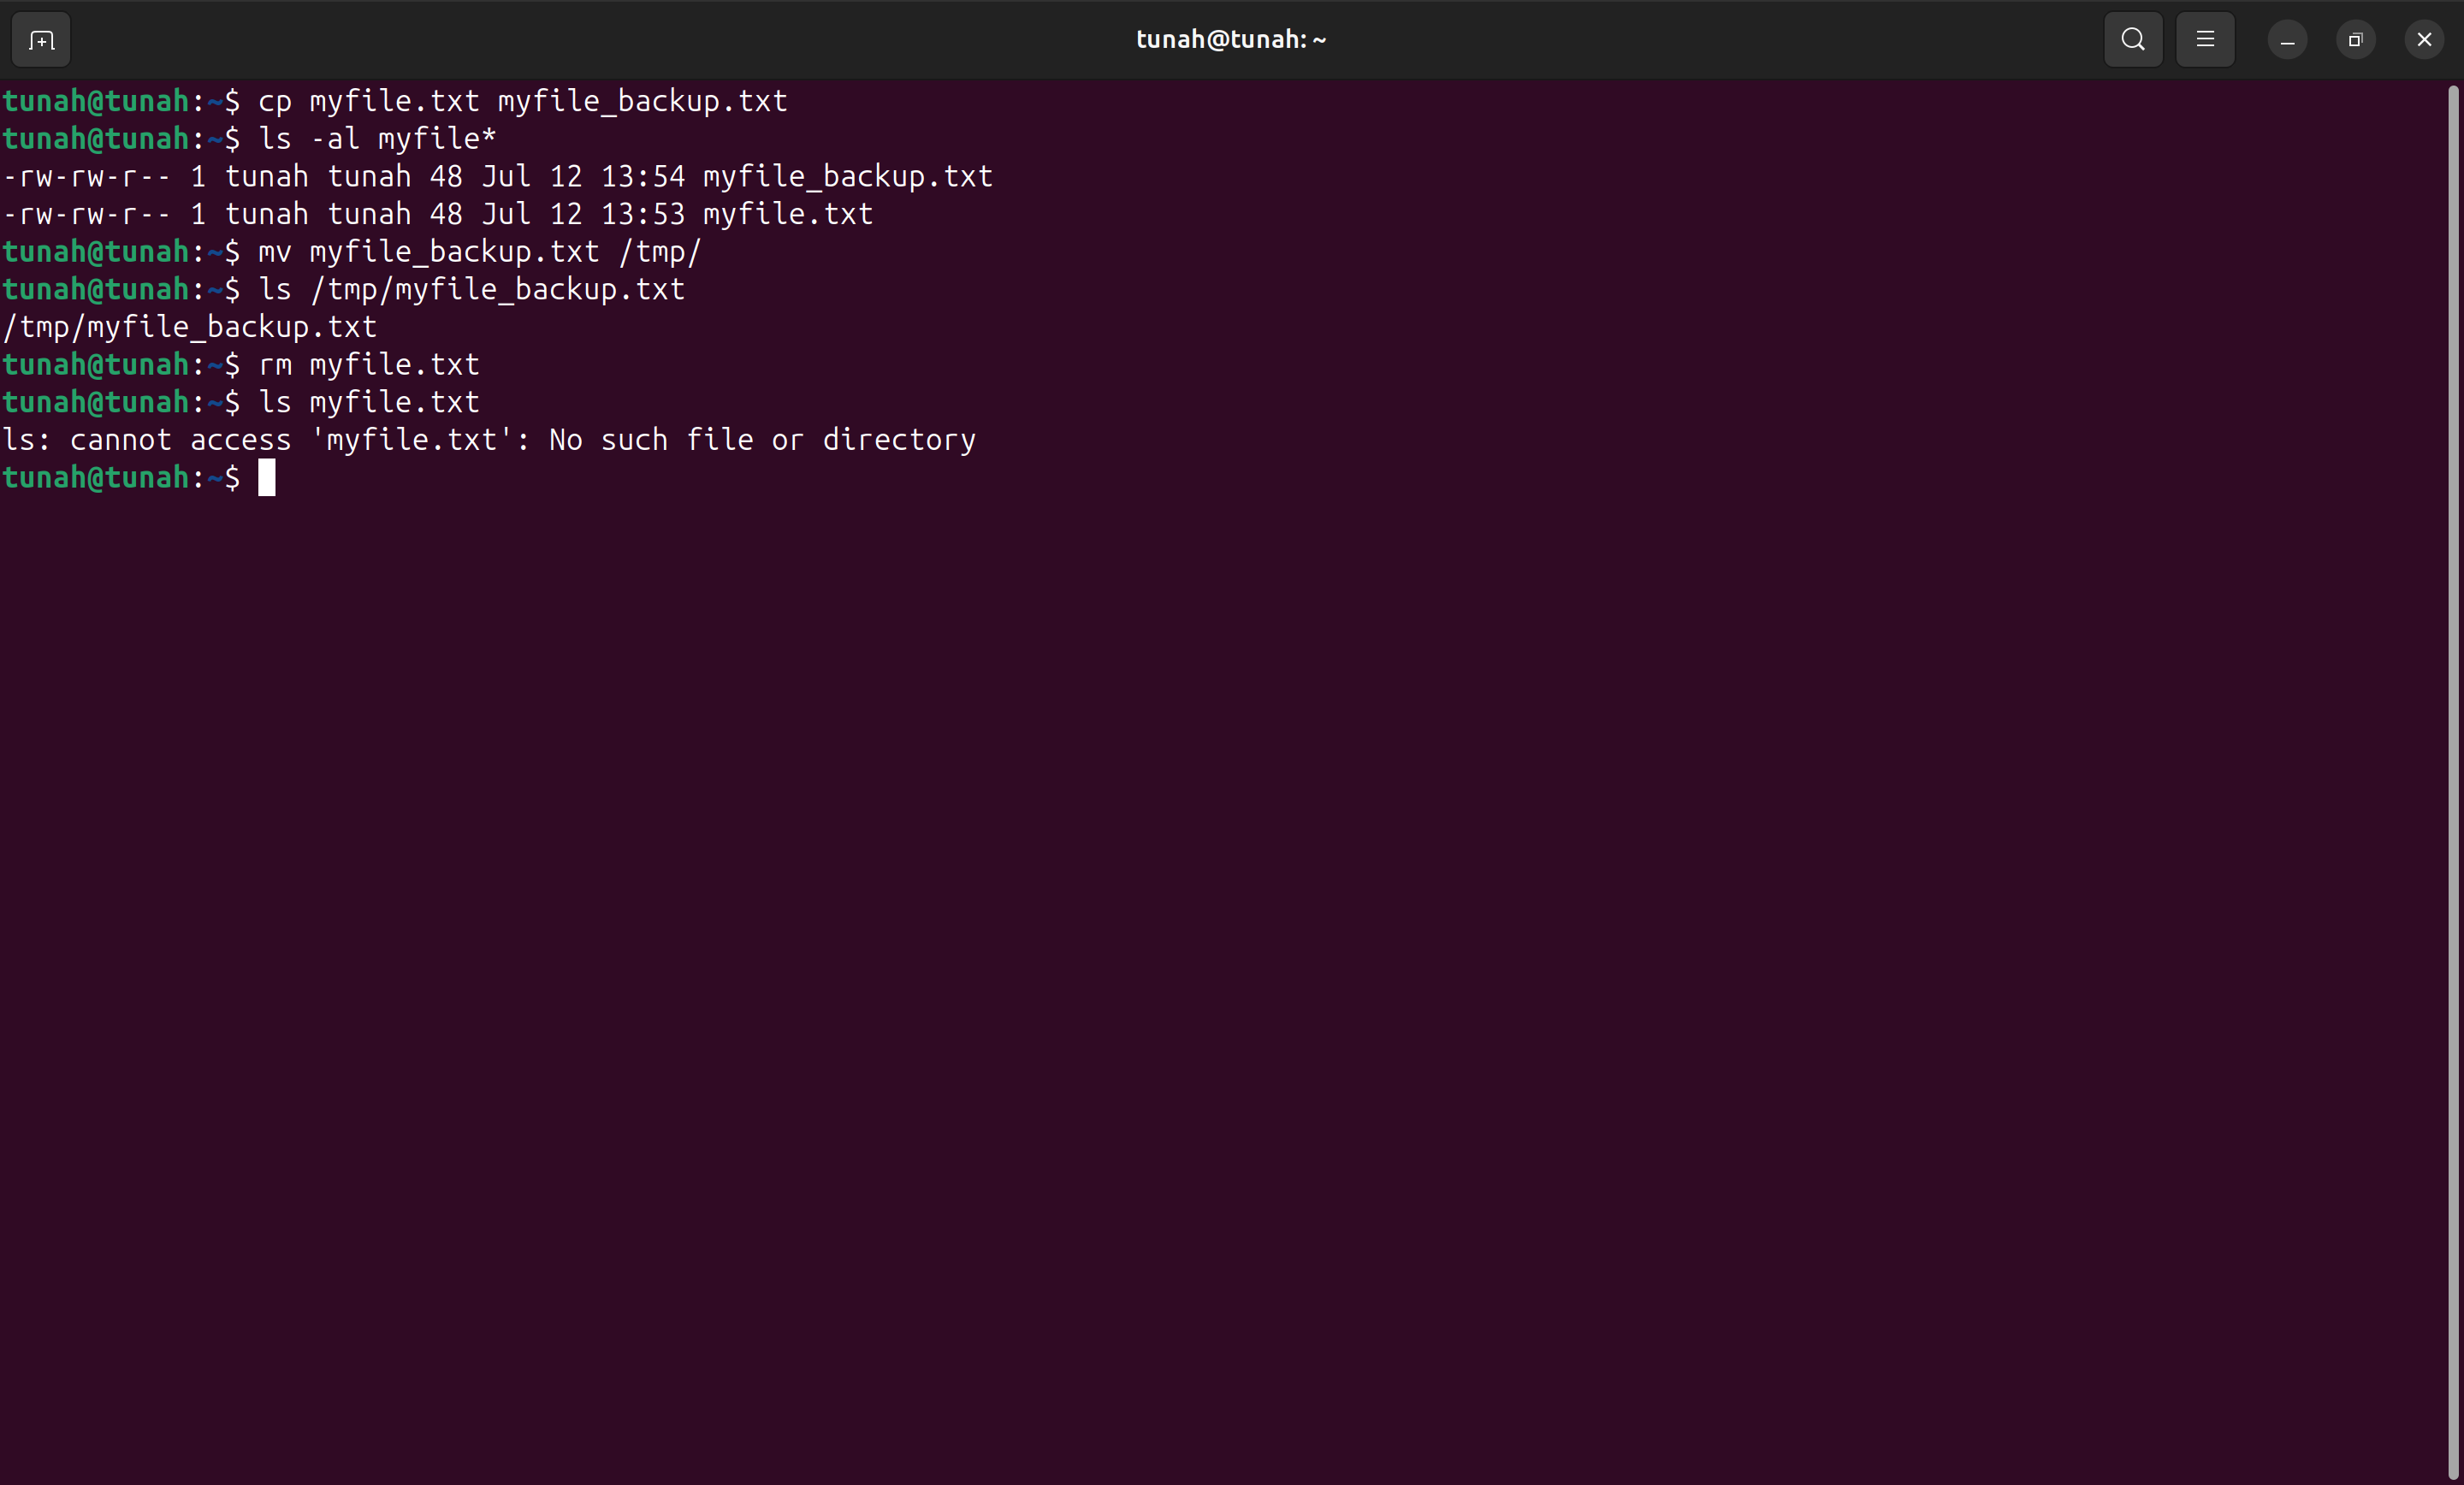
\includegraphics[width=\textwidth]{03/rm-myfile.png}
        \caption{Xóa file gốc}
    \end{subfigure}
    \caption{Thao tác quản lý File nâng cao}
\end{figure}

\subsection{Tìm kiếm, Đổi tên và Xem từng phần}

\textbf{Cách thực hiện:}
- Dùng \texttt{grep} để tìm kiếm chuỗi "Linux" trong file backup.
- Dùng \texttt{mv} để đổi tên file thành \texttt{linuxfile.txt}.
- Tạo thư mục \texttt{backup} và di chuyển file vào trong.
- Dùng \texttt{less} để xem nội dung file.

\begin{lstlisting}[language=bash]
# Tim kiem
grep "Linux" /tmp/myfile_backup.txt

# Doi ten va tao thu muc
mv /tmp/myfile_backup.txt /tmp/linuxfile.txt
mkdir backup
mv /tmp/linuxfile.txt backup/

# Xem noi dung tung trang
less backup/linuxfile.txt
\end{lstlisting}

\textbf{Kết quả:}
Công cụ \texttt{grep} tìm được đúng dòng chứa từ khóa. \texttt{mv} và \texttt{mkdir} tạo cấu trúc thư mục thành công.

\begin{figure}[H]
    \centering
    \begin{subfigure}[b]{0.45\textwidth}
        \centering
        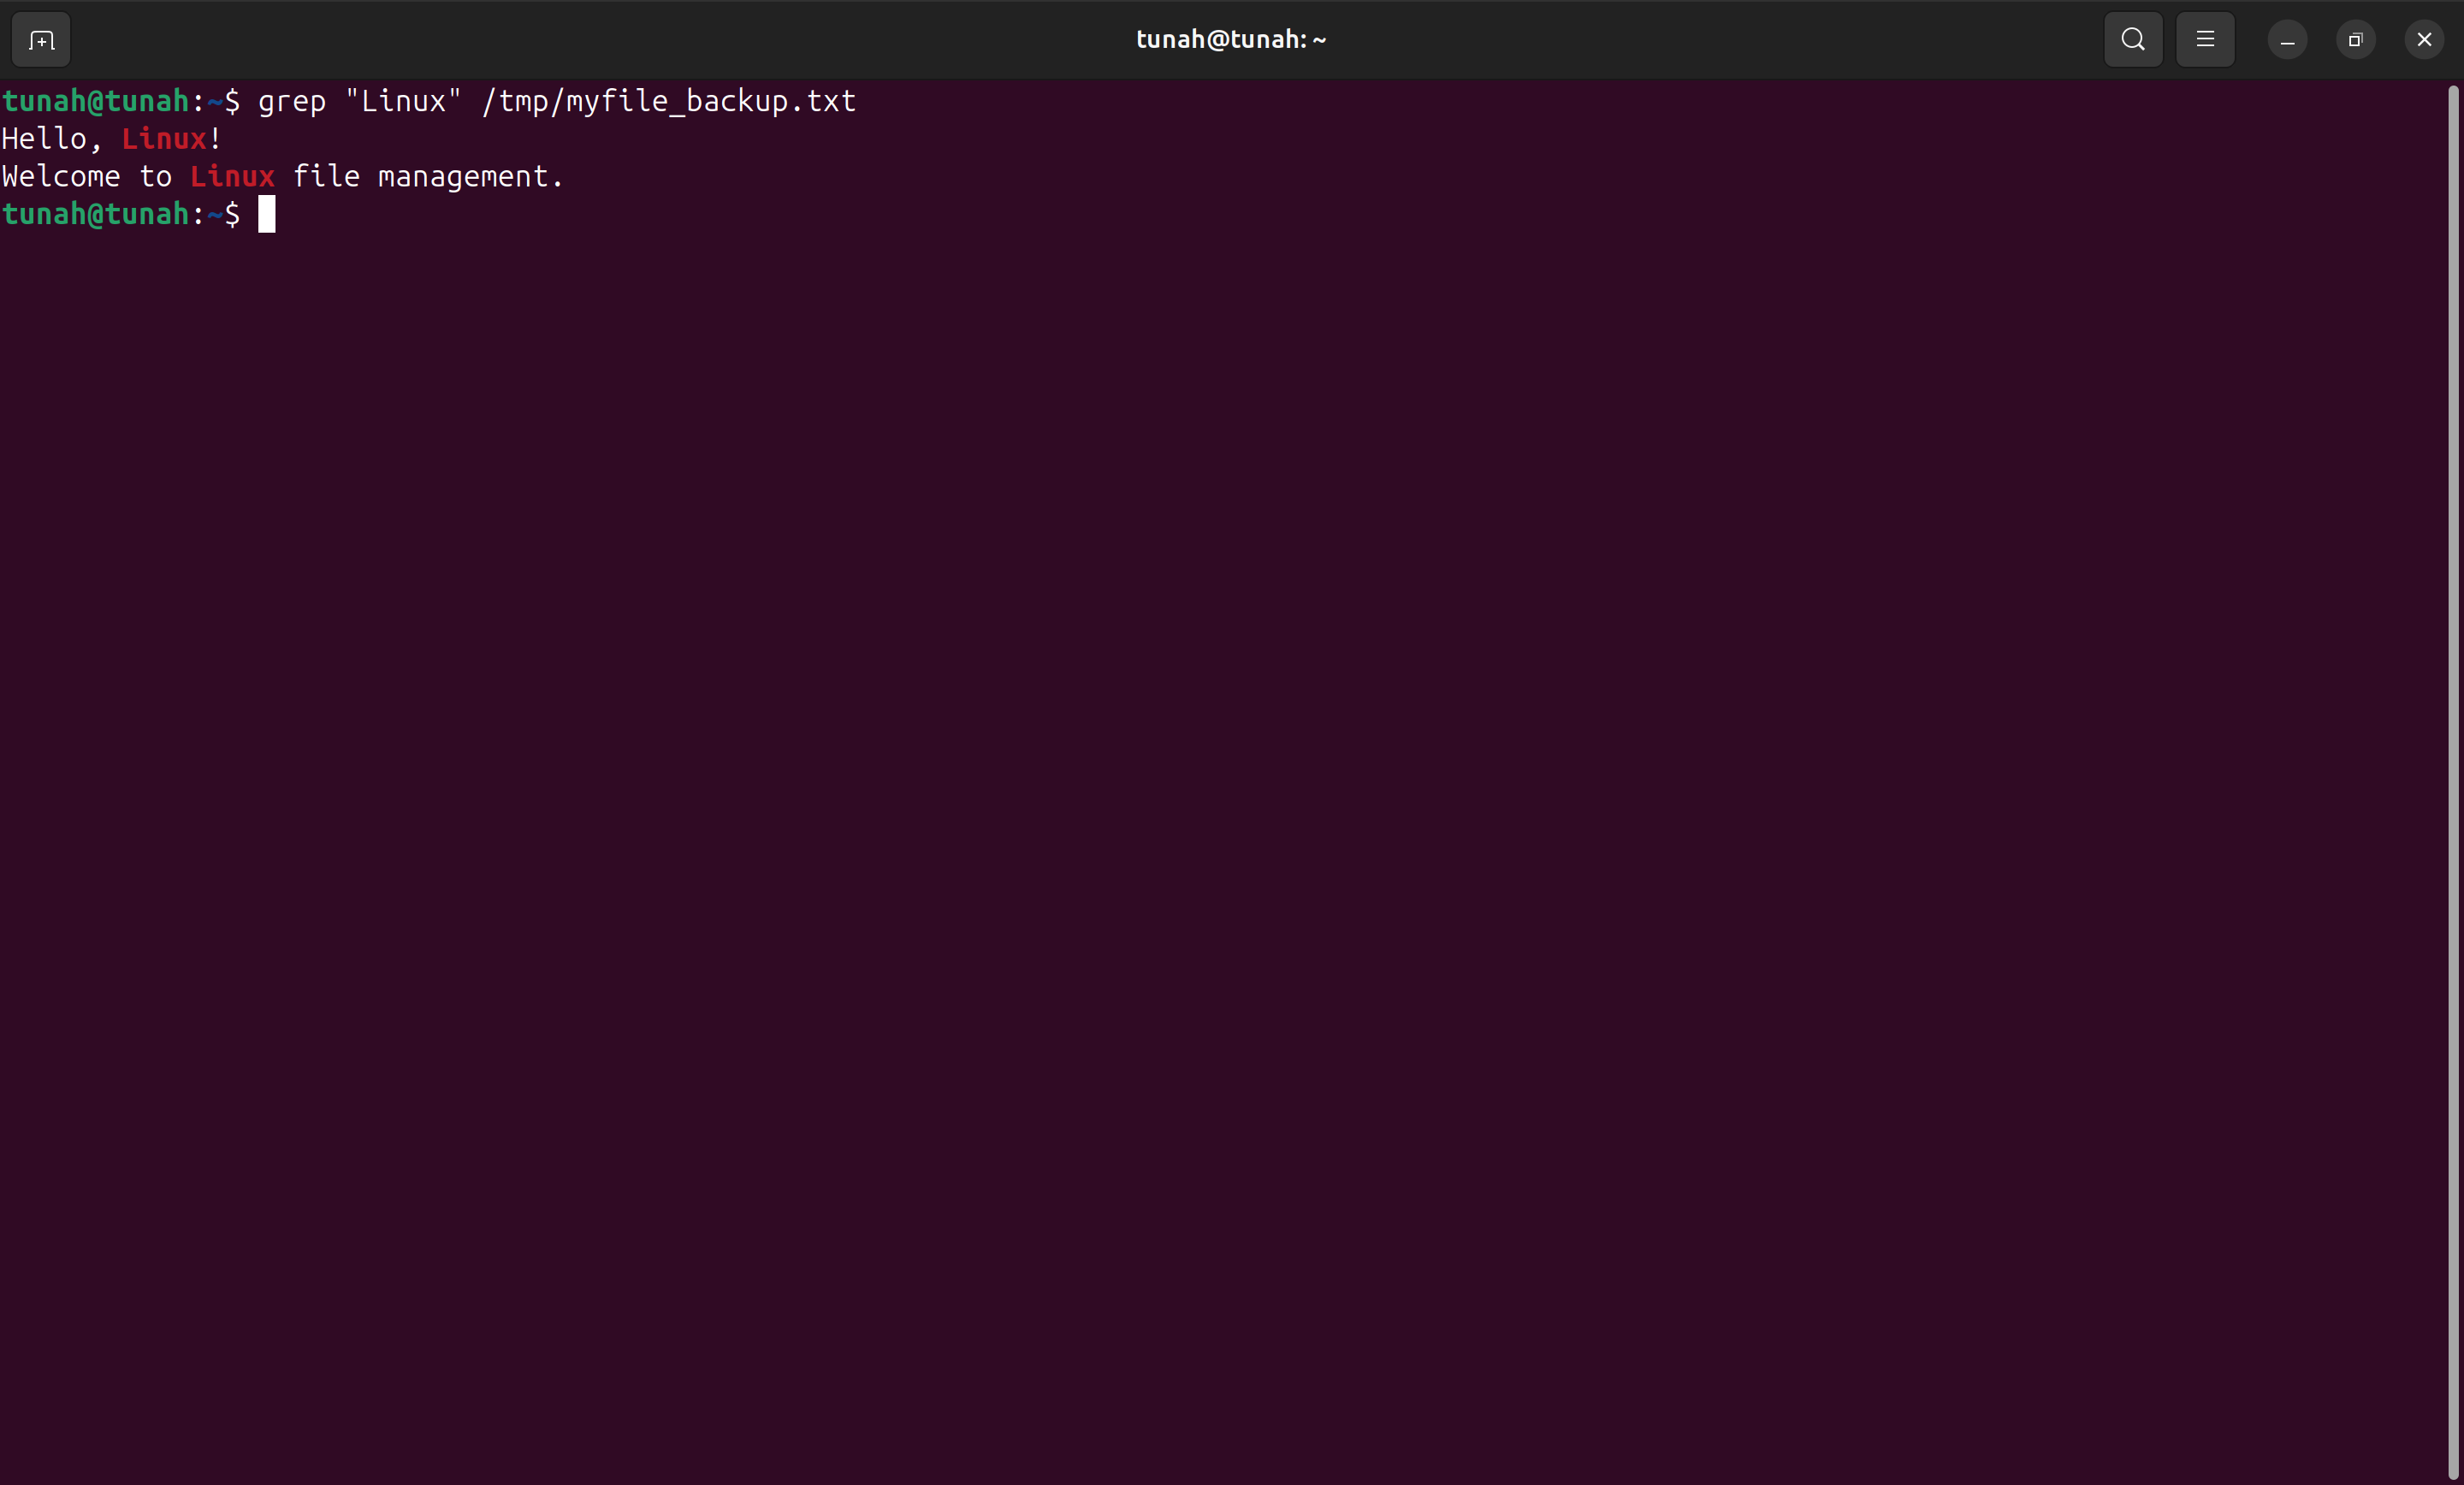
\includegraphics[width=\textwidth]{03/grep-linux.png}
        \caption{Tìm kiếm với grep}
    \end{subfigure}
    \hfill
    \begin{subfigure}[b]{0.45\textwidth}
        \centering
        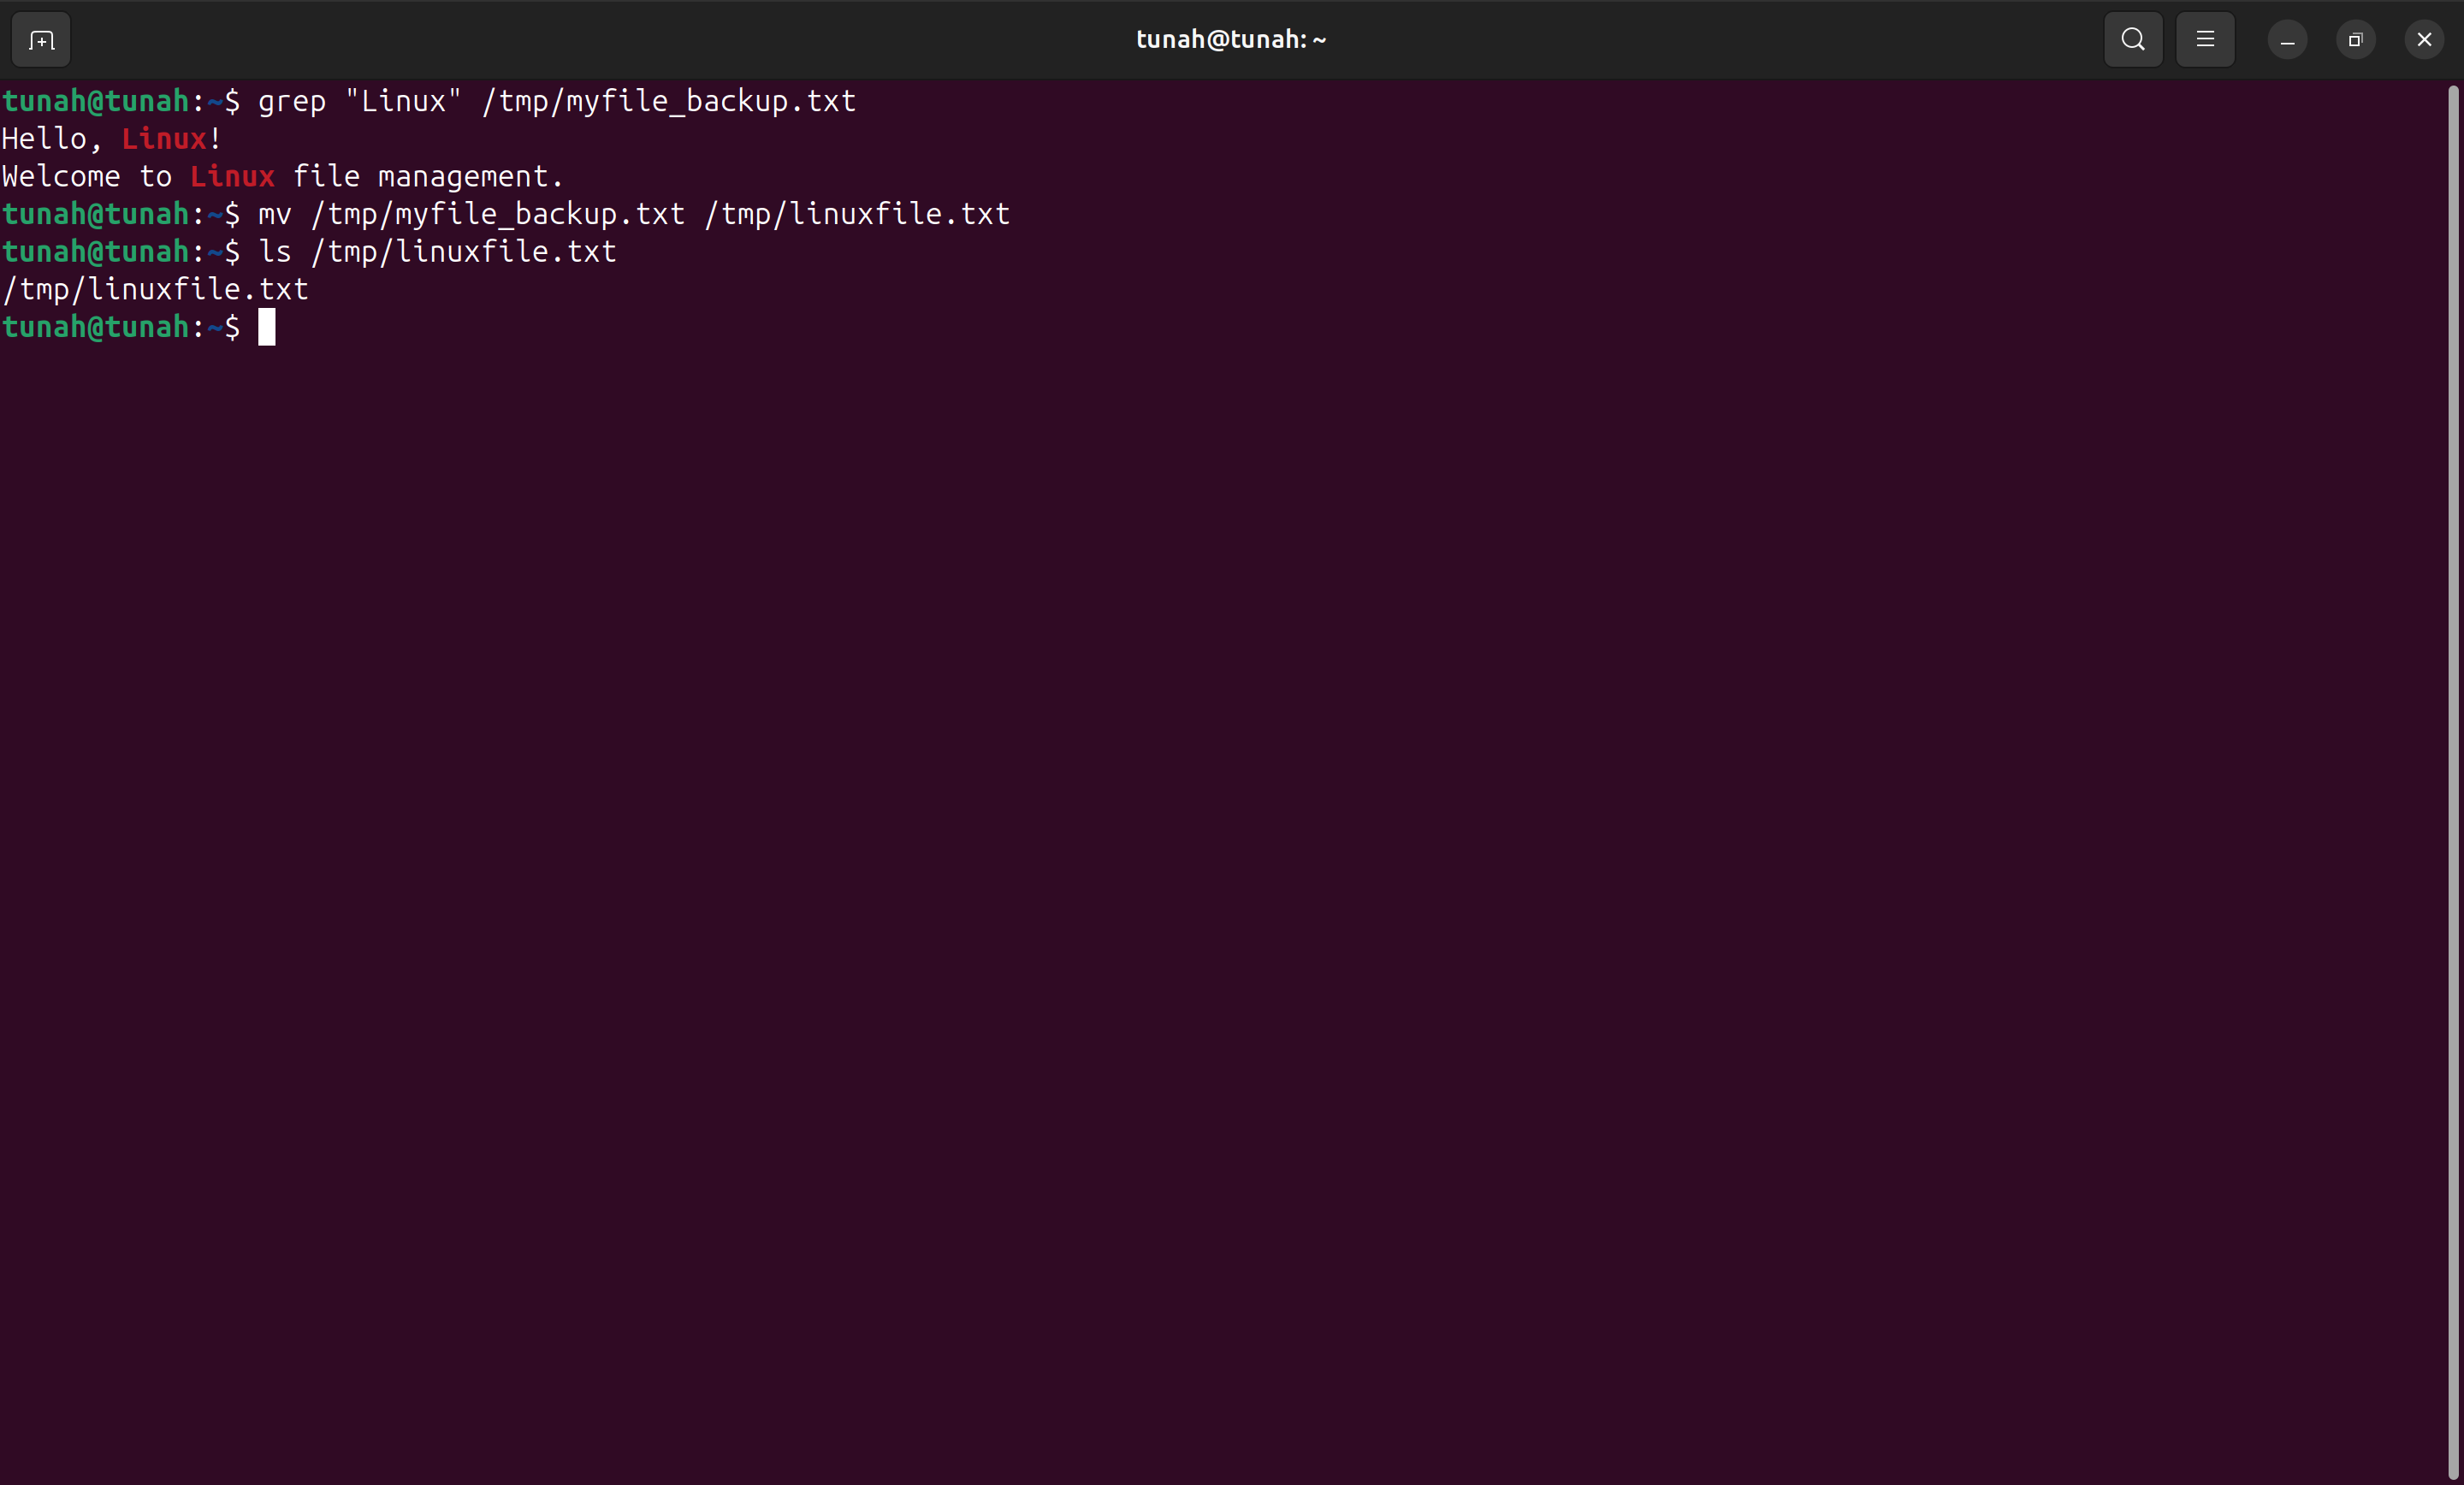
\includegraphics[width=\textwidth]{03/rename-linuxfile.png}
        \caption{Đổi tên file}
    \end{subfigure}
    
    \vspace{0.5cm}
    \begin{subfigure}[b]{0.45\textwidth}
        \centering
        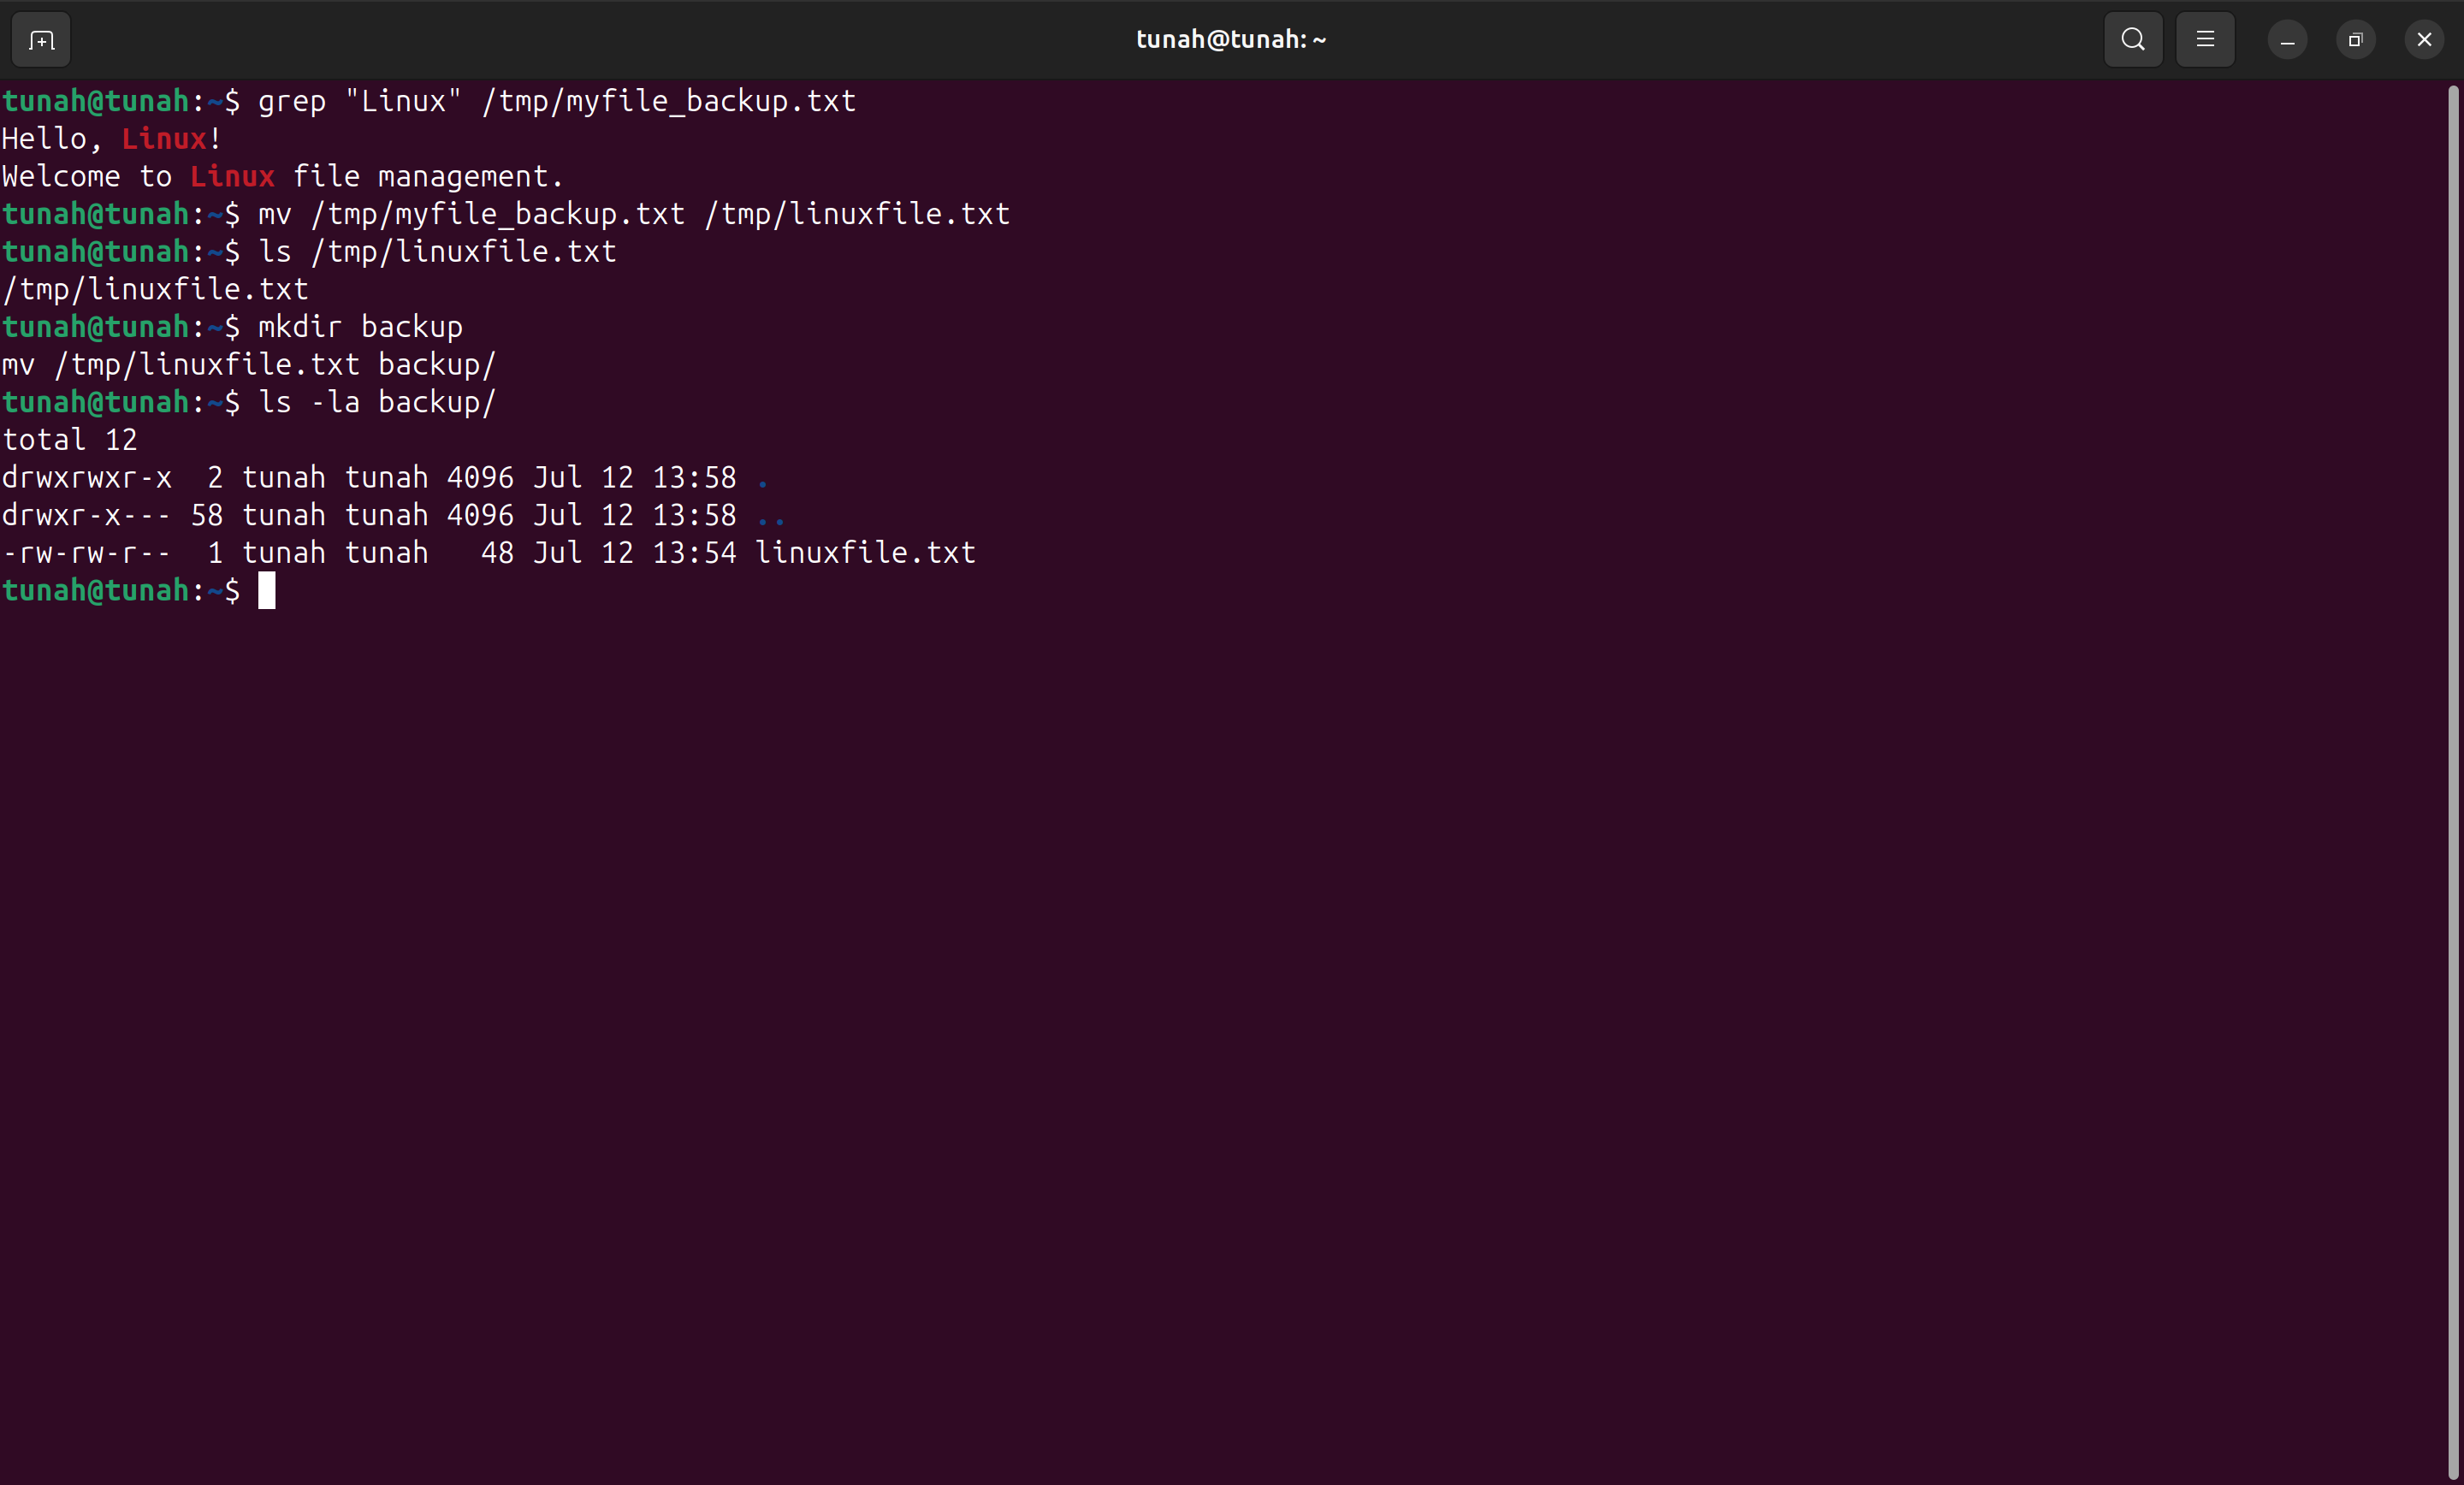
\includegraphics[width=\textwidth]{03/mkdir-backup-mv.png}
        \caption{Tạo thư mục và di chuyển}
    \end{subfigure}
    \hfill
    \begin{subfigure}[b]{0.45\textwidth}
        \centering
        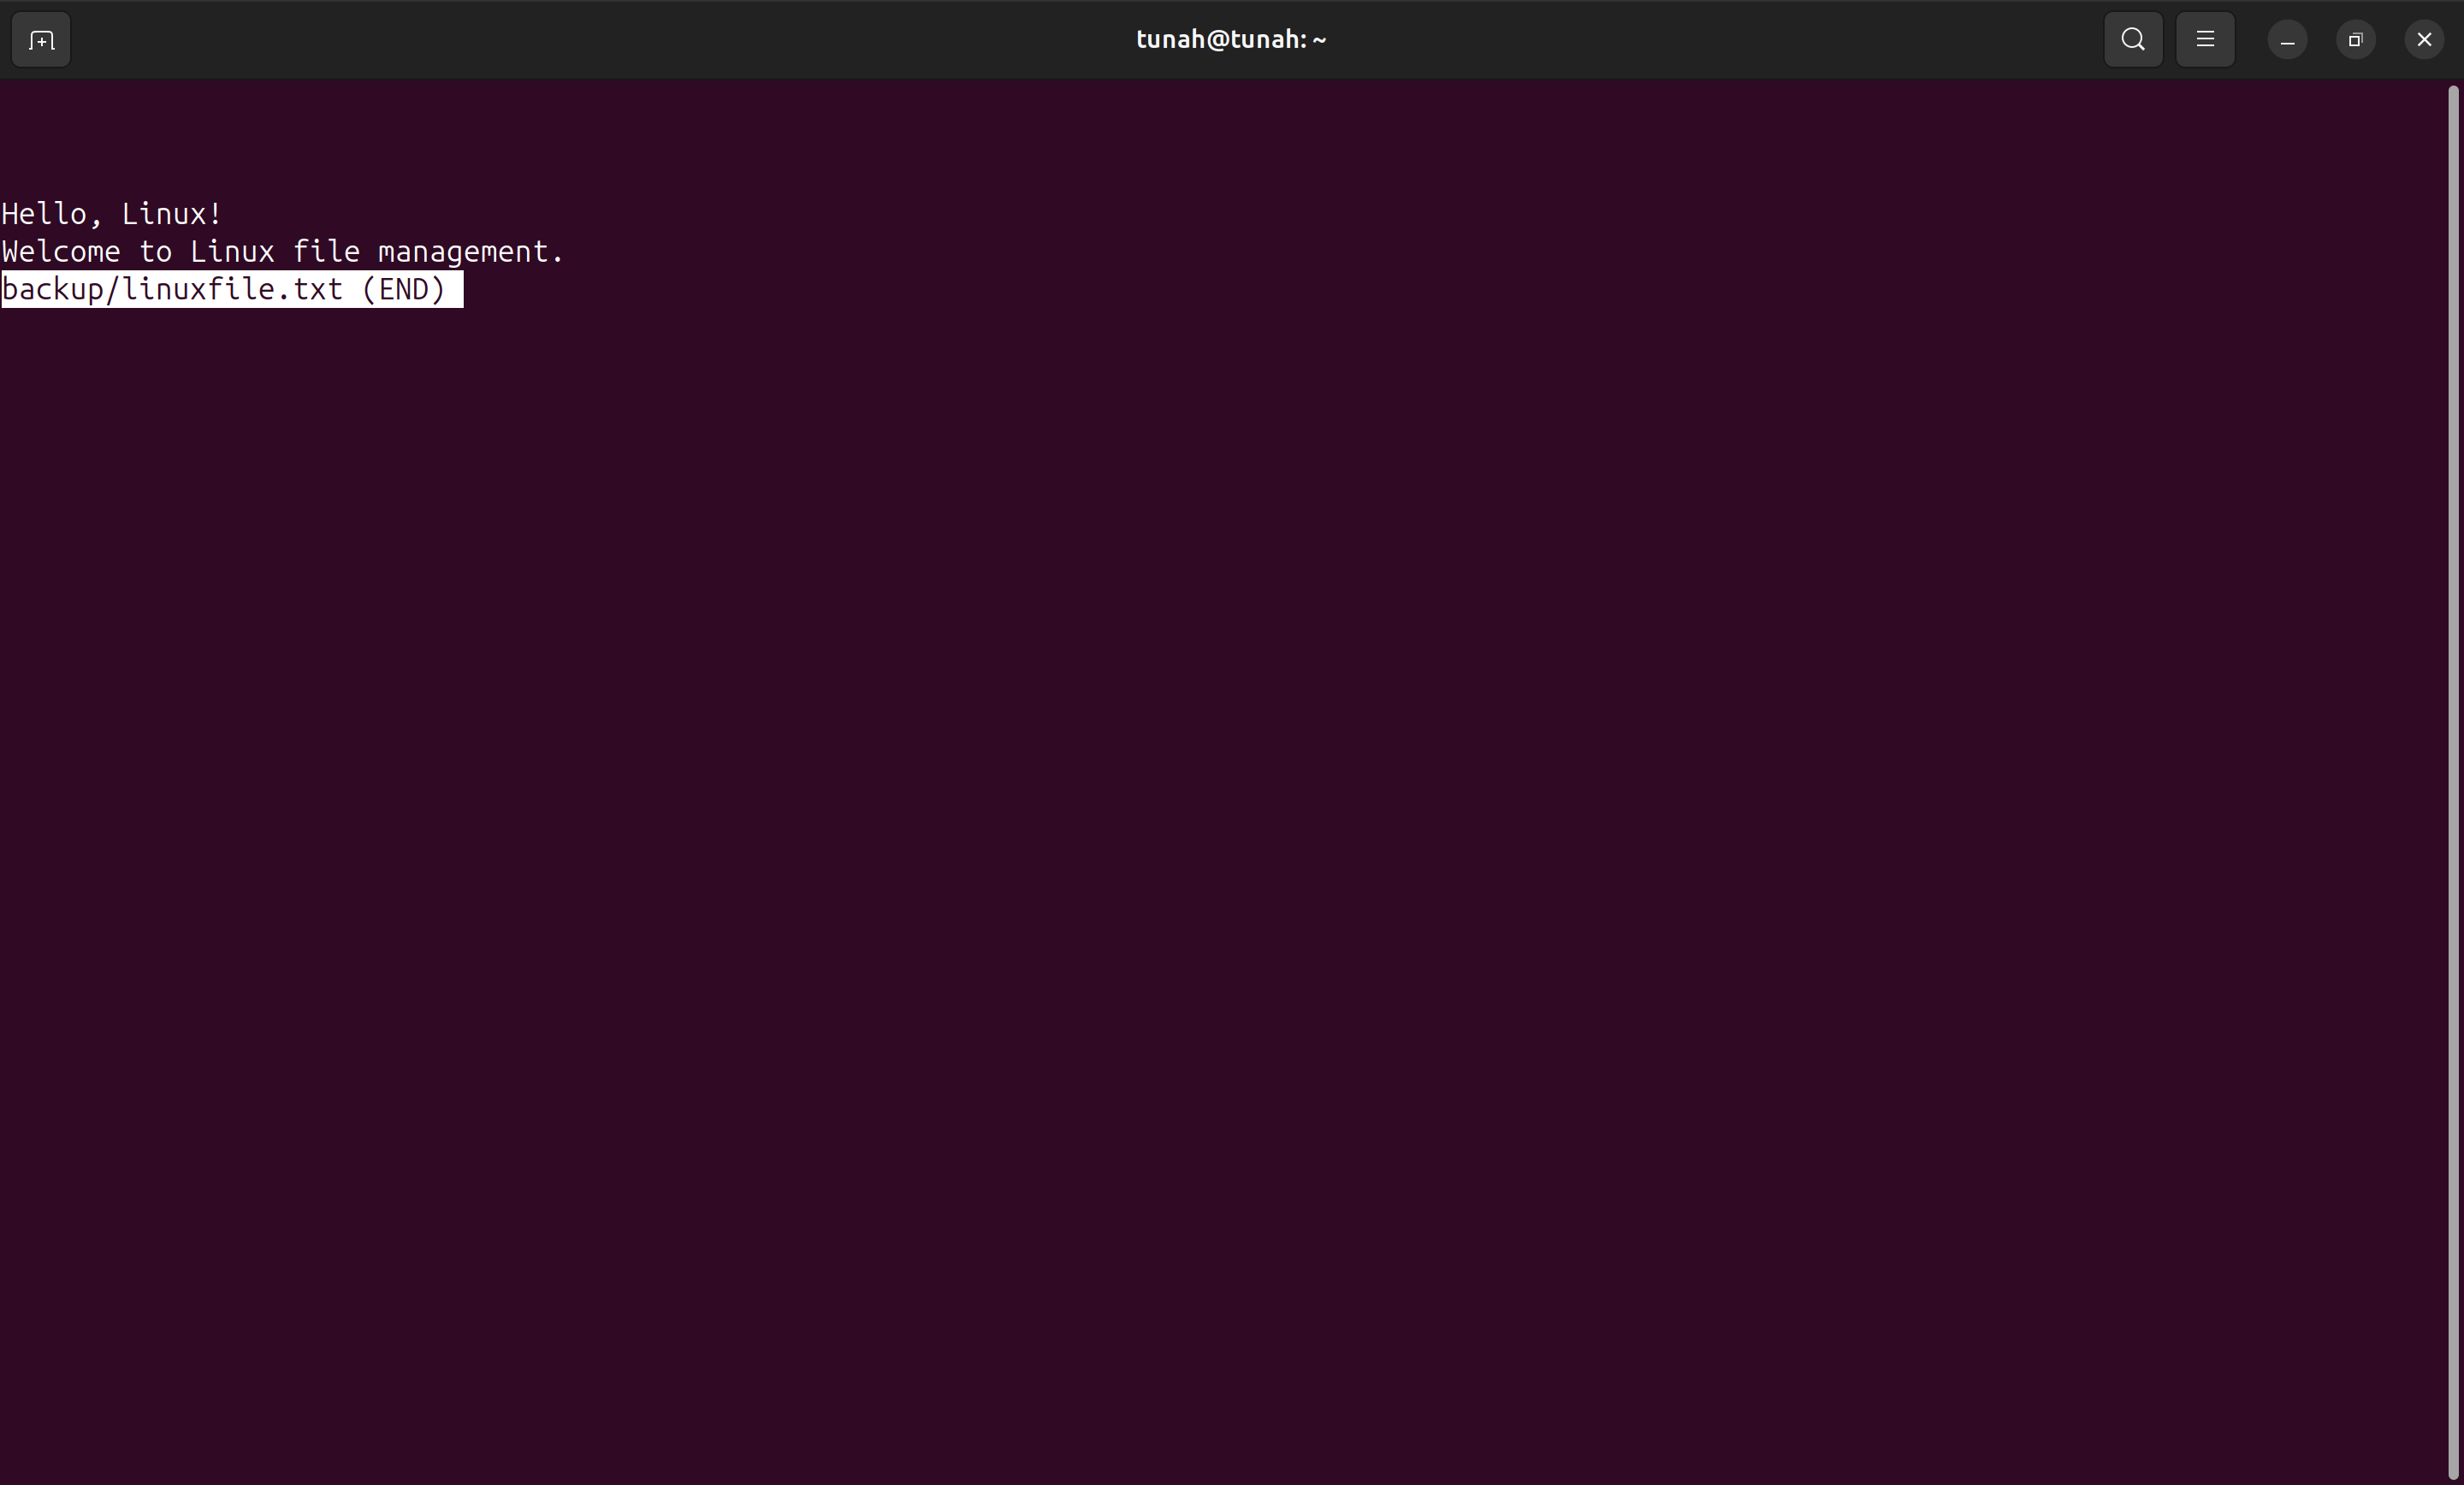
\includegraphics[width=\textwidth]{03/less-linuxfile.png}
        \caption{Xem file bằng less}
    \end{subfigure}
    \caption{Các công cụ tìm kiếm và điều hướng}
\end{figure}

\section{Quản lý Gói Phần mềm (Package Management)}

\subsection{Cập nhật và Cài đặt gói phần mềm}

\textbf{Cách thực hiện:}
Tiến hành cập nhật danh sách các gói phần mềm trên hệ thống với lệnh \texttt{update}, sau đó cài đặt dịch vụ \texttt{vsftpd}.

\begin{lstlisting}[language=bash]
# Cap nhat danh sach
sudo apt update

# Cai dat vsftpd
sudo apt install vsftpd -y
\end{lstlisting}

\textbf{Kết quả:}
Hệ thống lấy danh sách thành công và tự động tải về, cài đặt gói \texttt{vsftpd}.

\begin{figure}[H]
    \centering
    \begin{subfigure}[b]{0.48\textwidth}
        \centering
        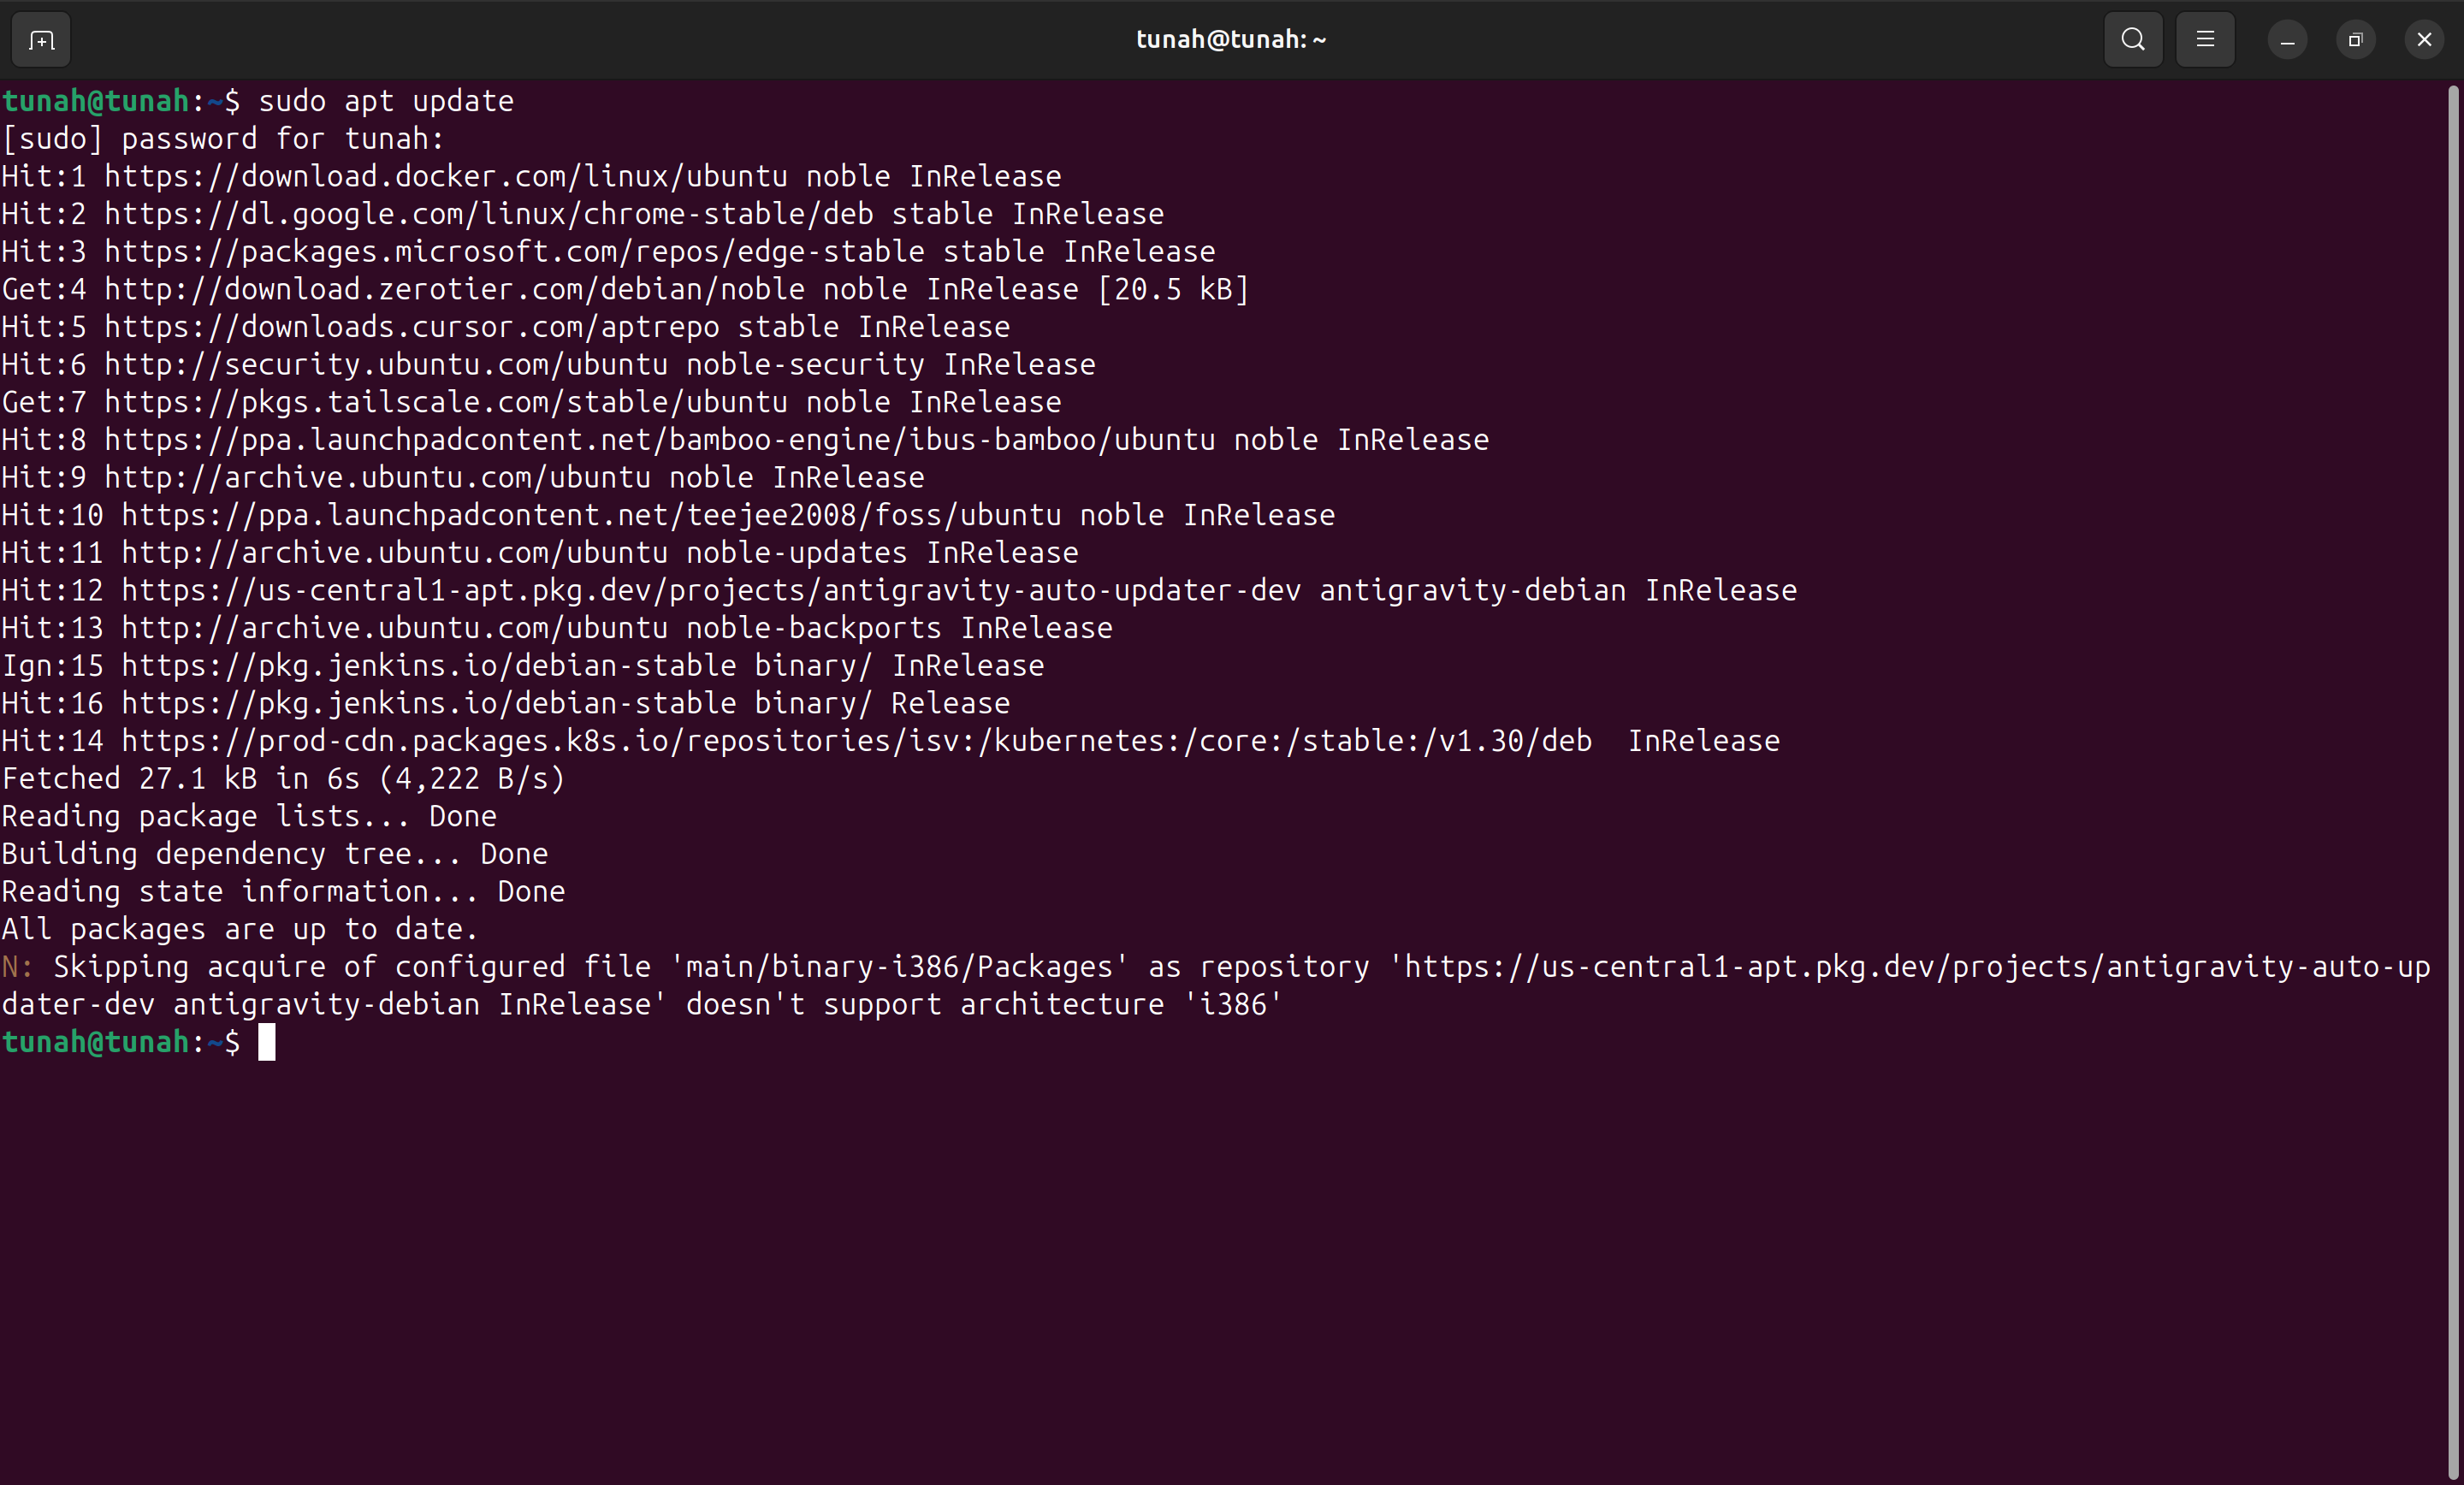
\includegraphics[width=\textwidth]{04/apt-update.png}
        \caption{Cập nhật APT}
    \end{subfigure}
    \hfill
    \begin{subfigure}[b]{0.48\textwidth}
        \centering
        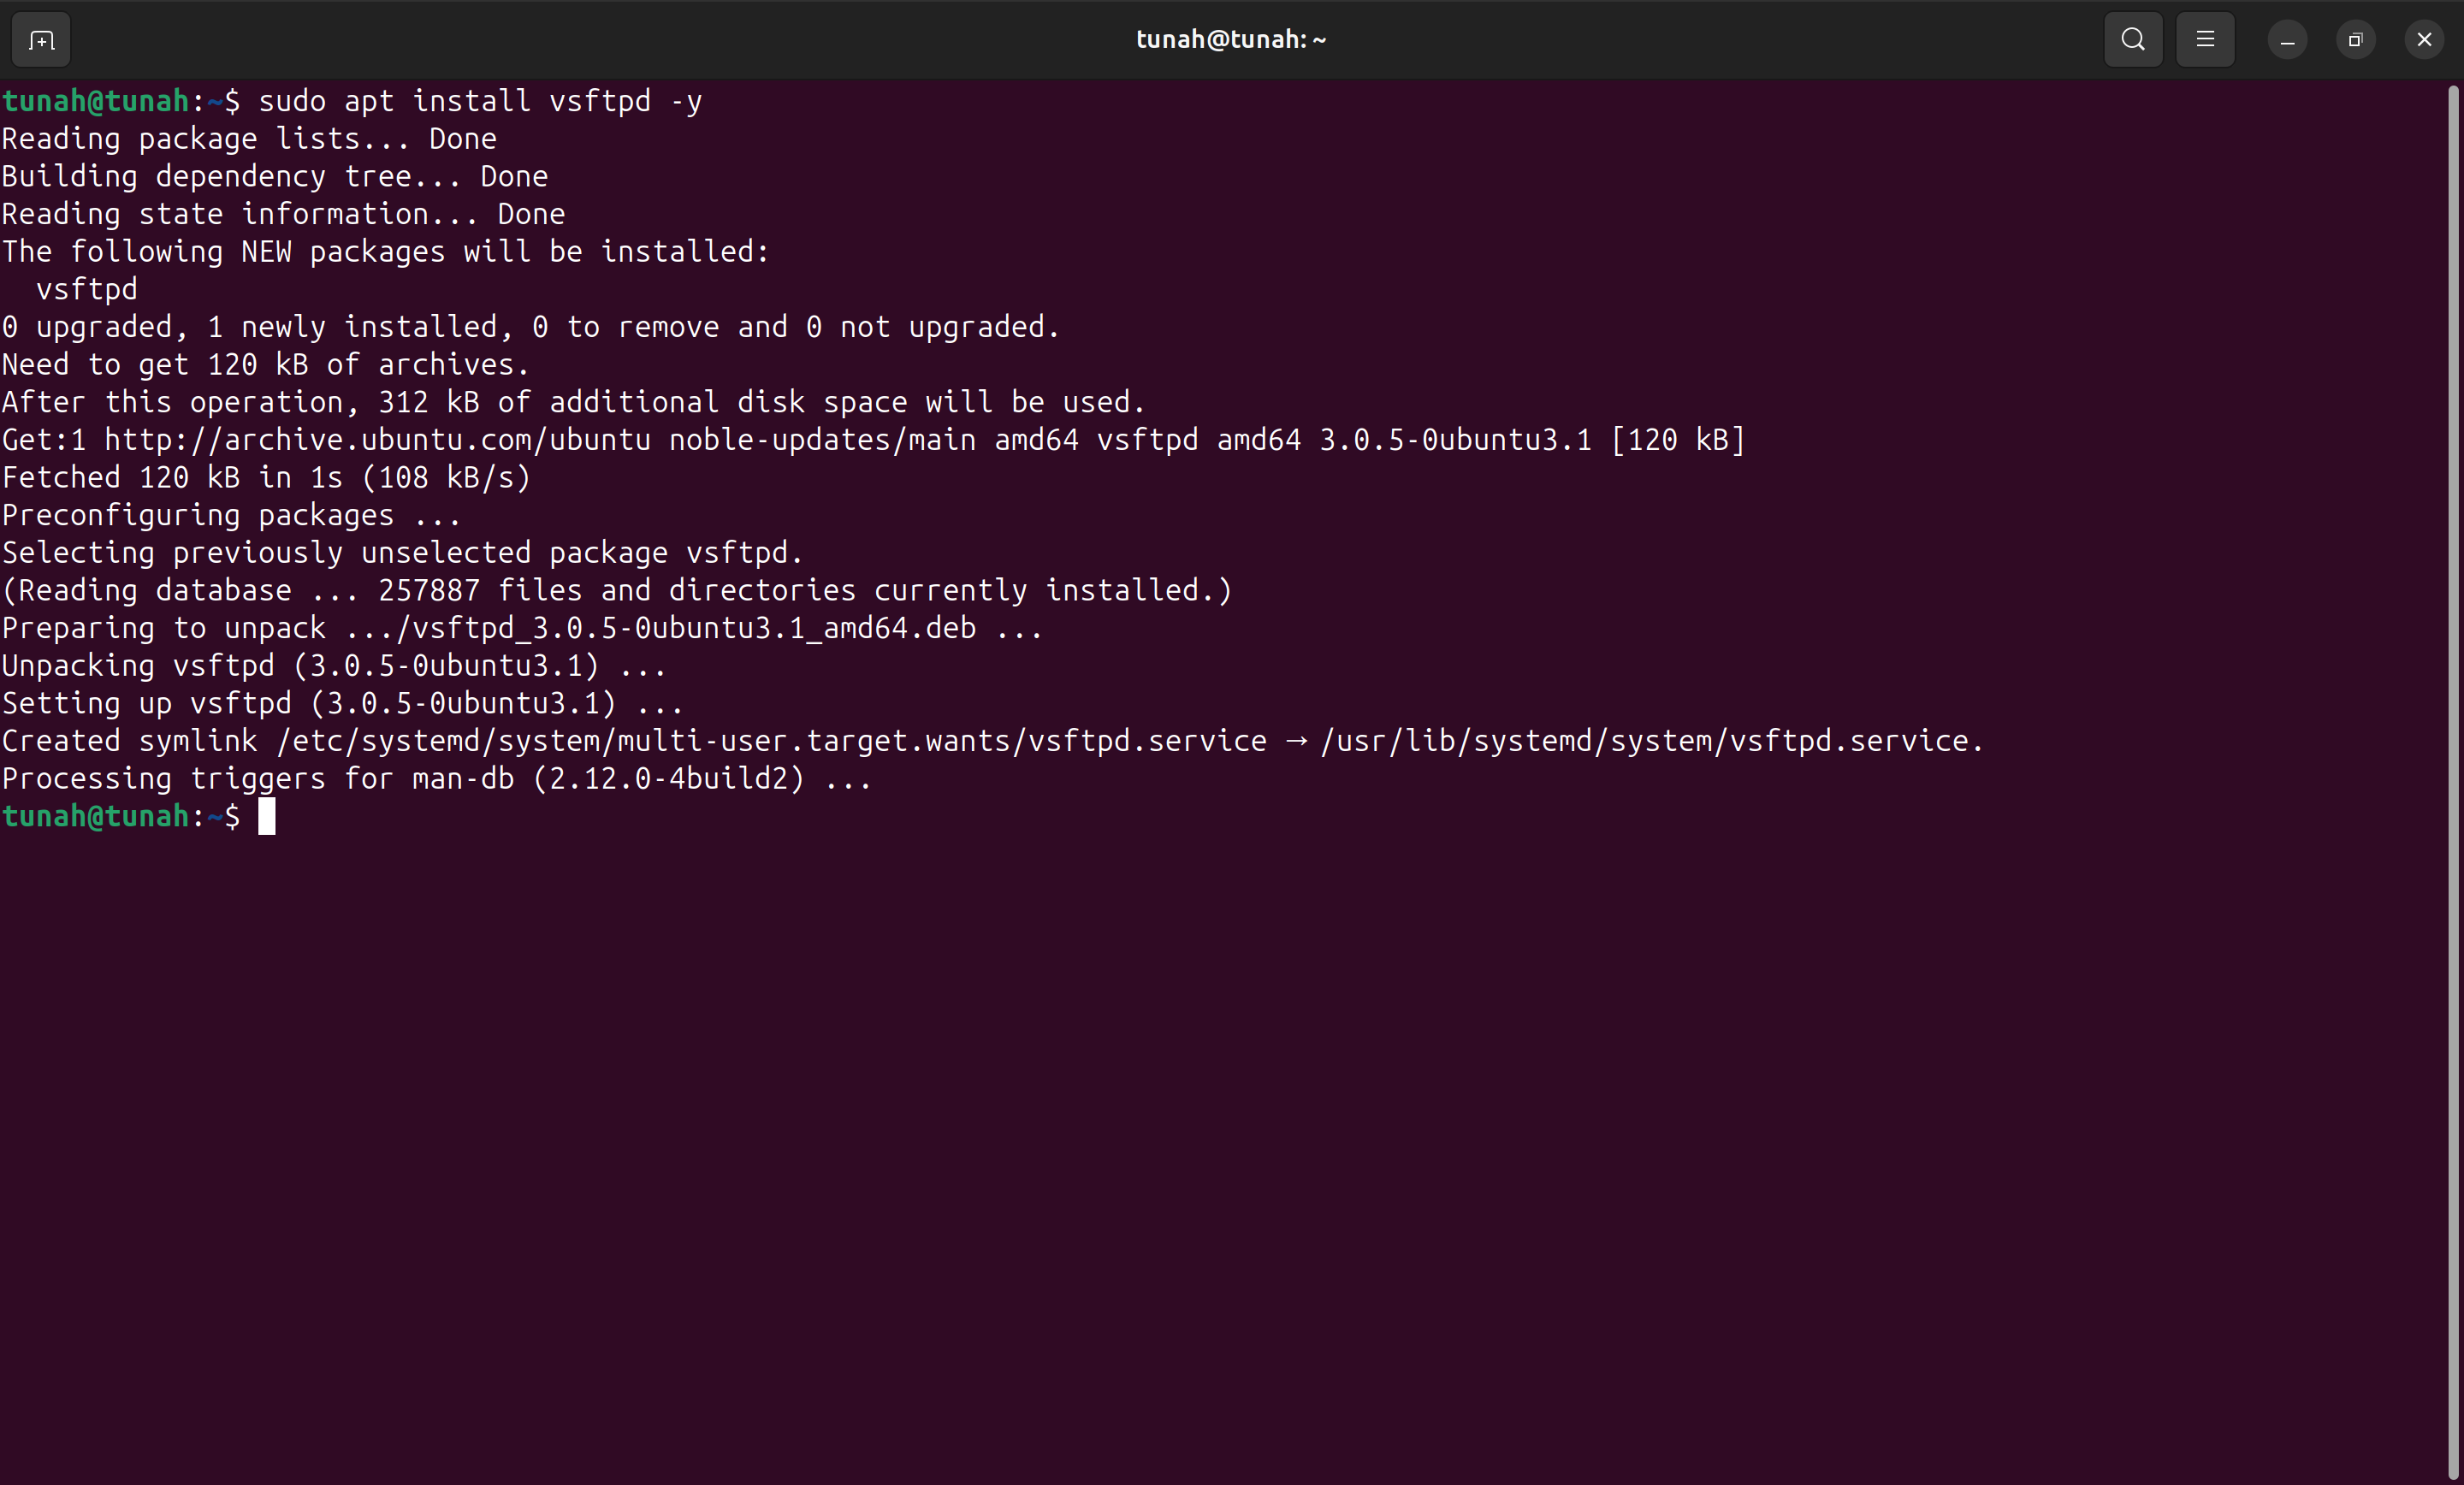
\includegraphics[width=\textwidth]{04/apt-install-vsftpd.png}
        \caption{Cài đặt vsftpd}
    \end{subfigure}
    \caption{Cập nhật và cài đặt phần mềm}
\end{figure}

\subsection{Tìm kiếm, Xem chi tiết và Gỡ bỏ}

\textbf{Cách thực hiện:}
- Tìm kiếm từ khóa \texttt{net-tools} trong kho lưu trữ.
- Hiển thị thông tin chi tiết về gói \texttt{vsftpd} vừa cài.
- Thực hiện lệnh xóa hoàn toàn \texttt{vsftpd} khỏi hệ thống.

\begin{lstlisting}[language=bash]
apt search net-tools
apt show vsftpd
sudo apt remove vsftpd -y
\end{lstlisting}

\textbf{Kết quả:}
Các lệnh trả về chính xác kết quả tìm kiếm và thông tin package. Lệnh \texttt{remove} gỡ bỏ thành công.

\begin{figure}[H]
    \centering
    \begin{subfigure}[b]{0.48\textwidth}
        \centering
        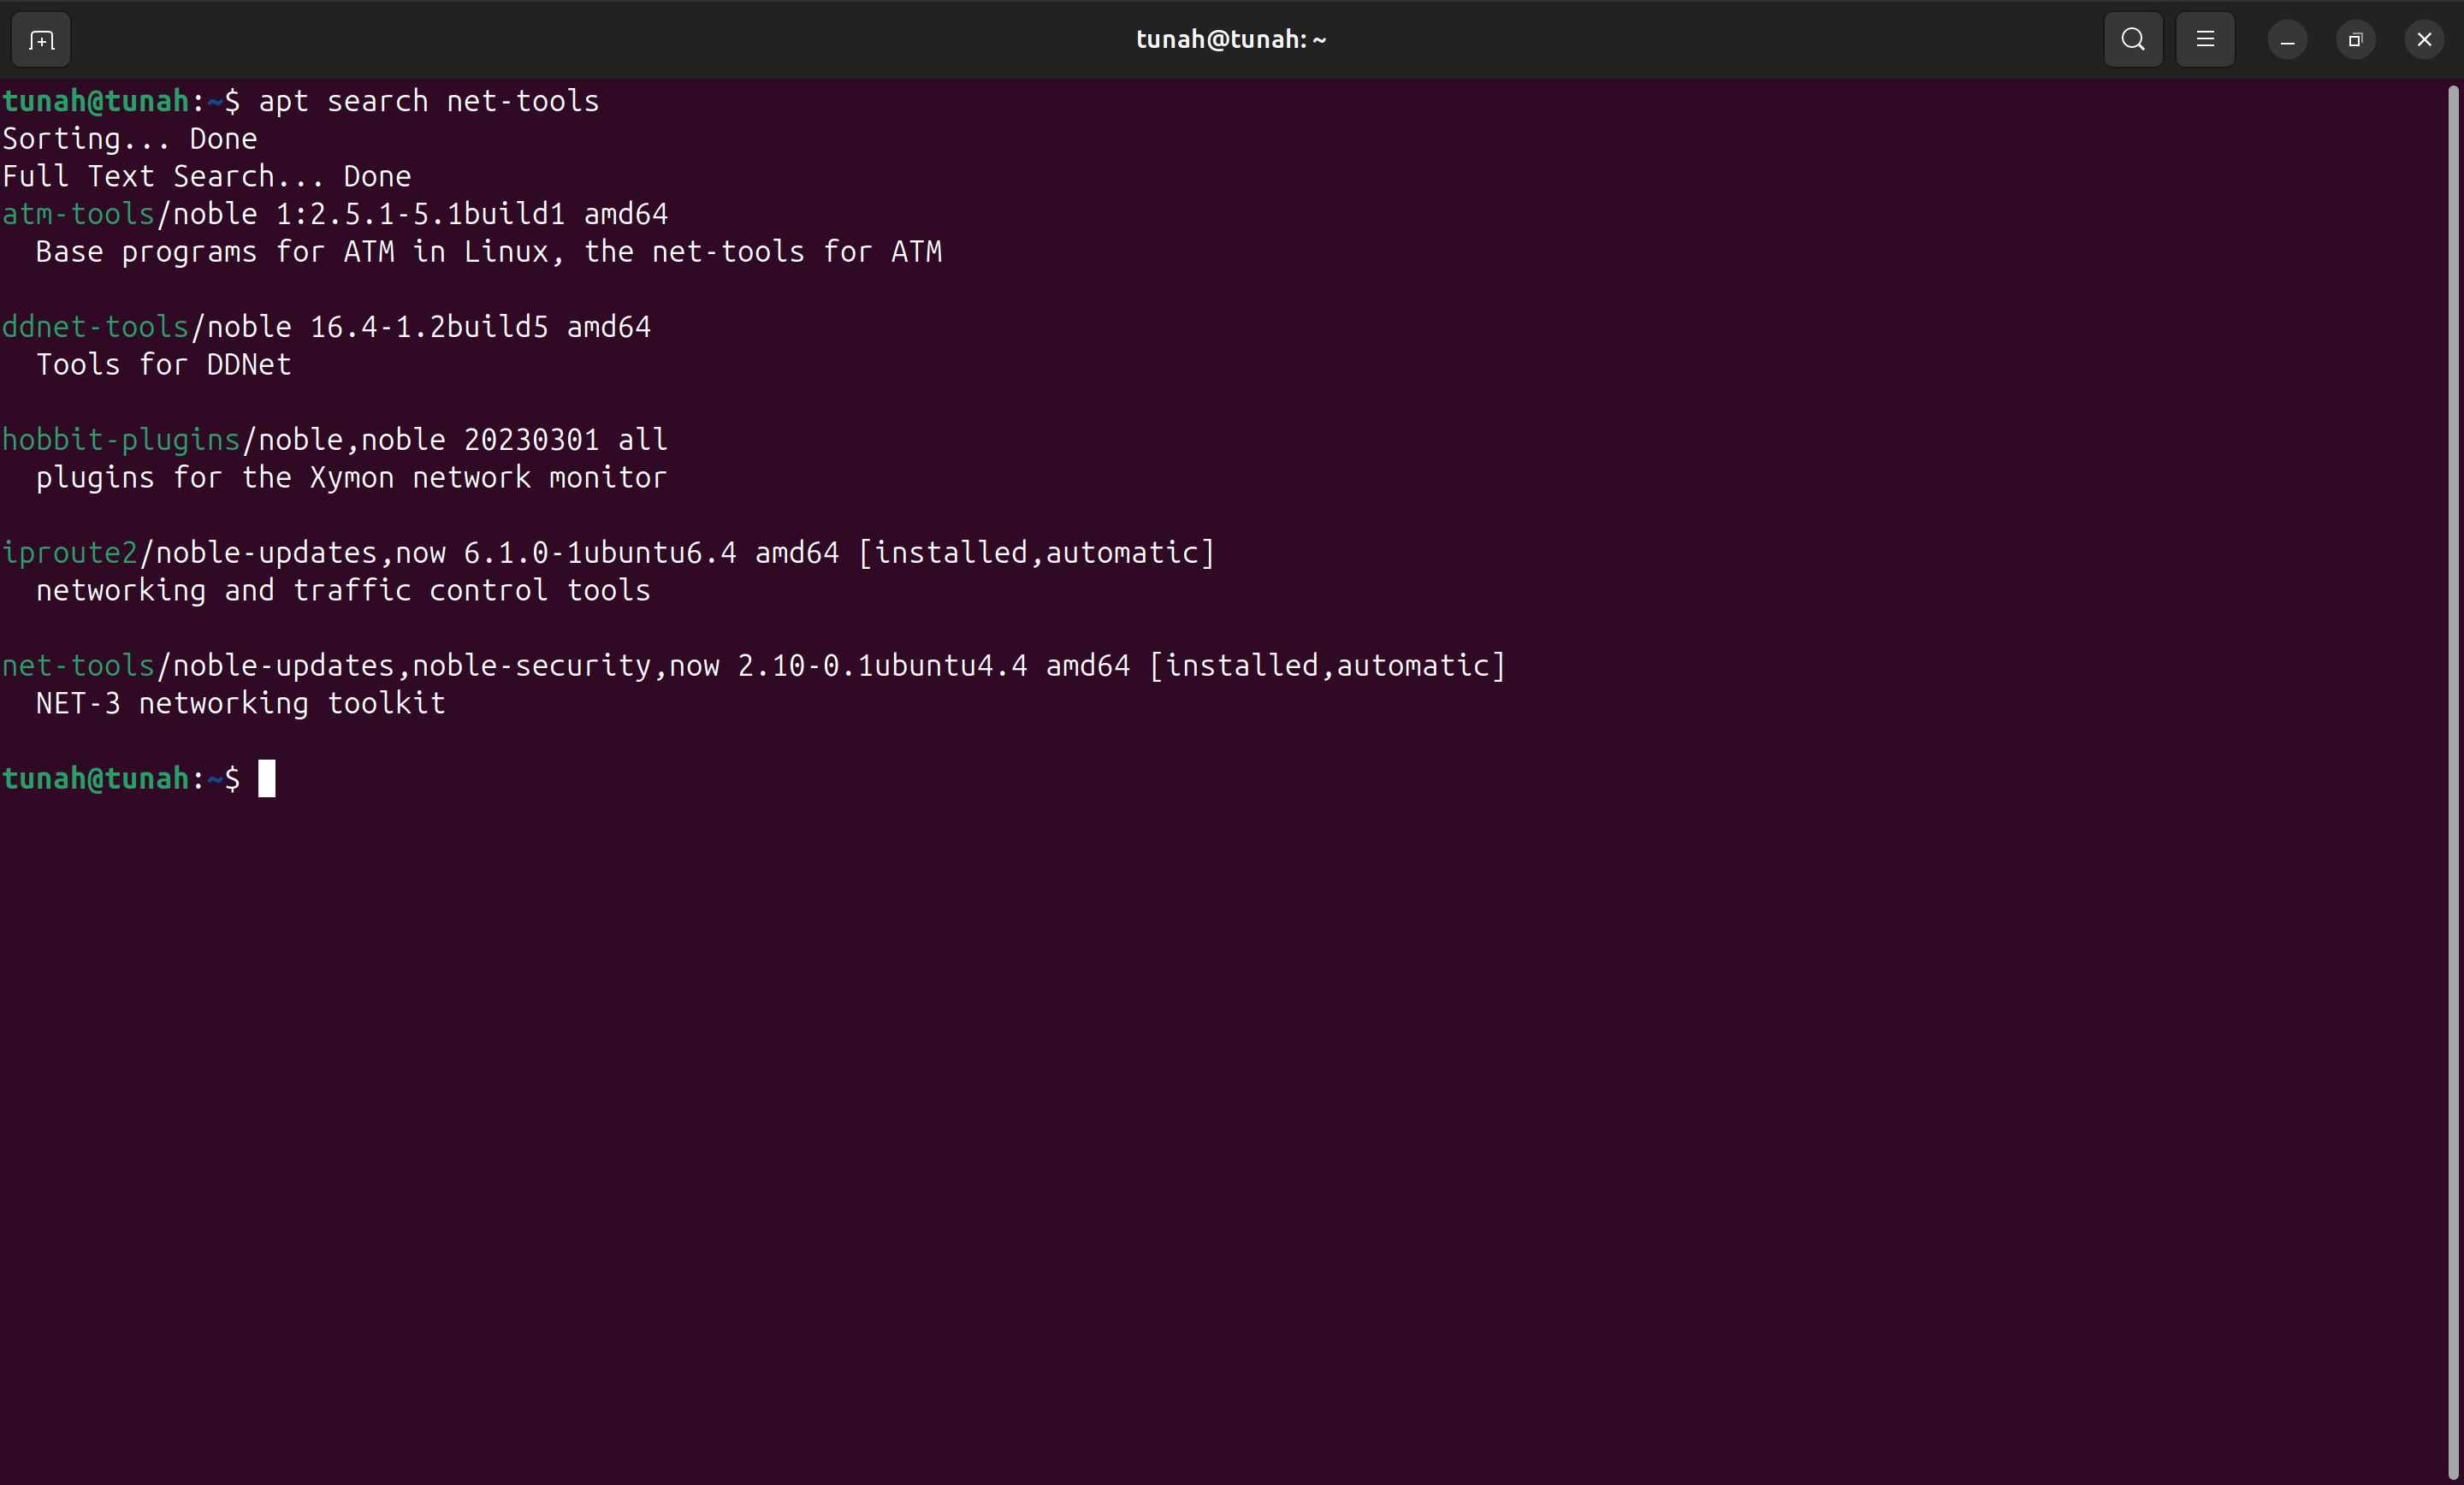
\includegraphics[width=\textwidth]{04/apt-search-nettools.png}
        \caption{Tìm kiếm net-tools}
    \end{subfigure}
    \hfill
    \begin{subfigure}[b]{0.48\textwidth}
        \centering
        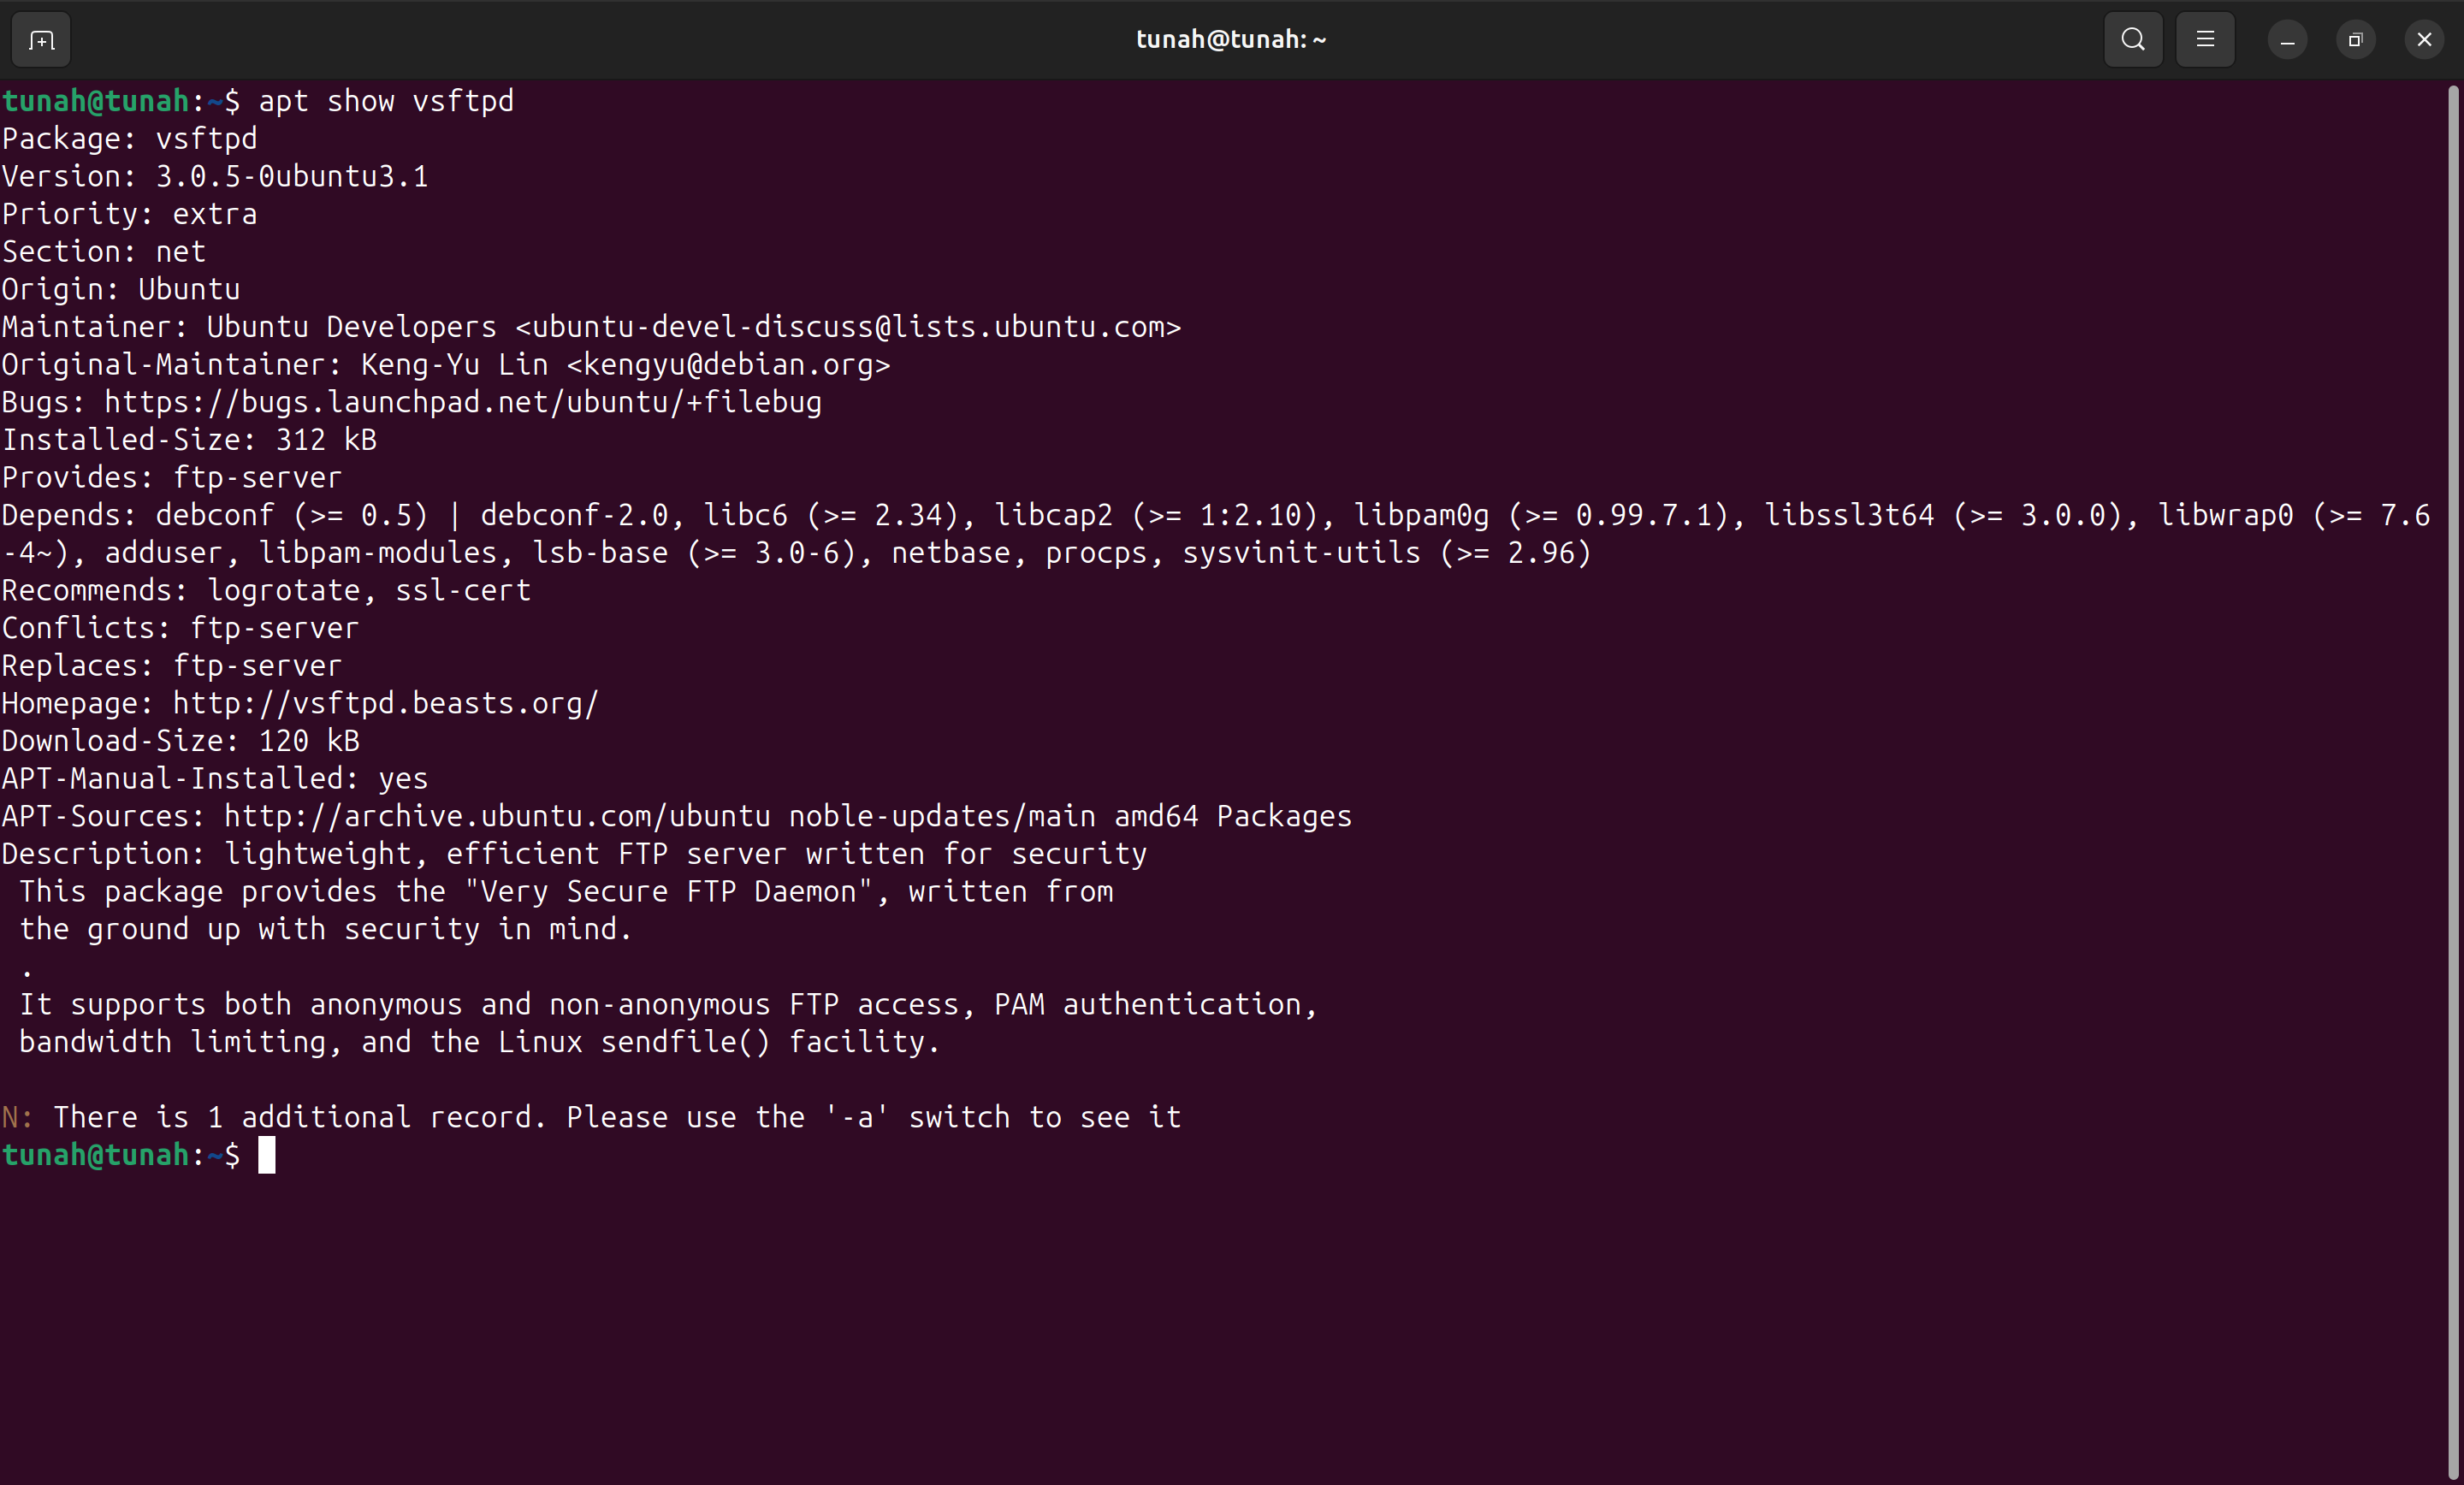
\includegraphics[width=\textwidth]{04/apt-show-vsftpd.png}
        \caption{Xem chi tiết vsftpd}
    \end{subfigure}
    
    \vspace{0.5cm}
    \begin{subfigure}[b]{0.48\textwidth}
        \centering
        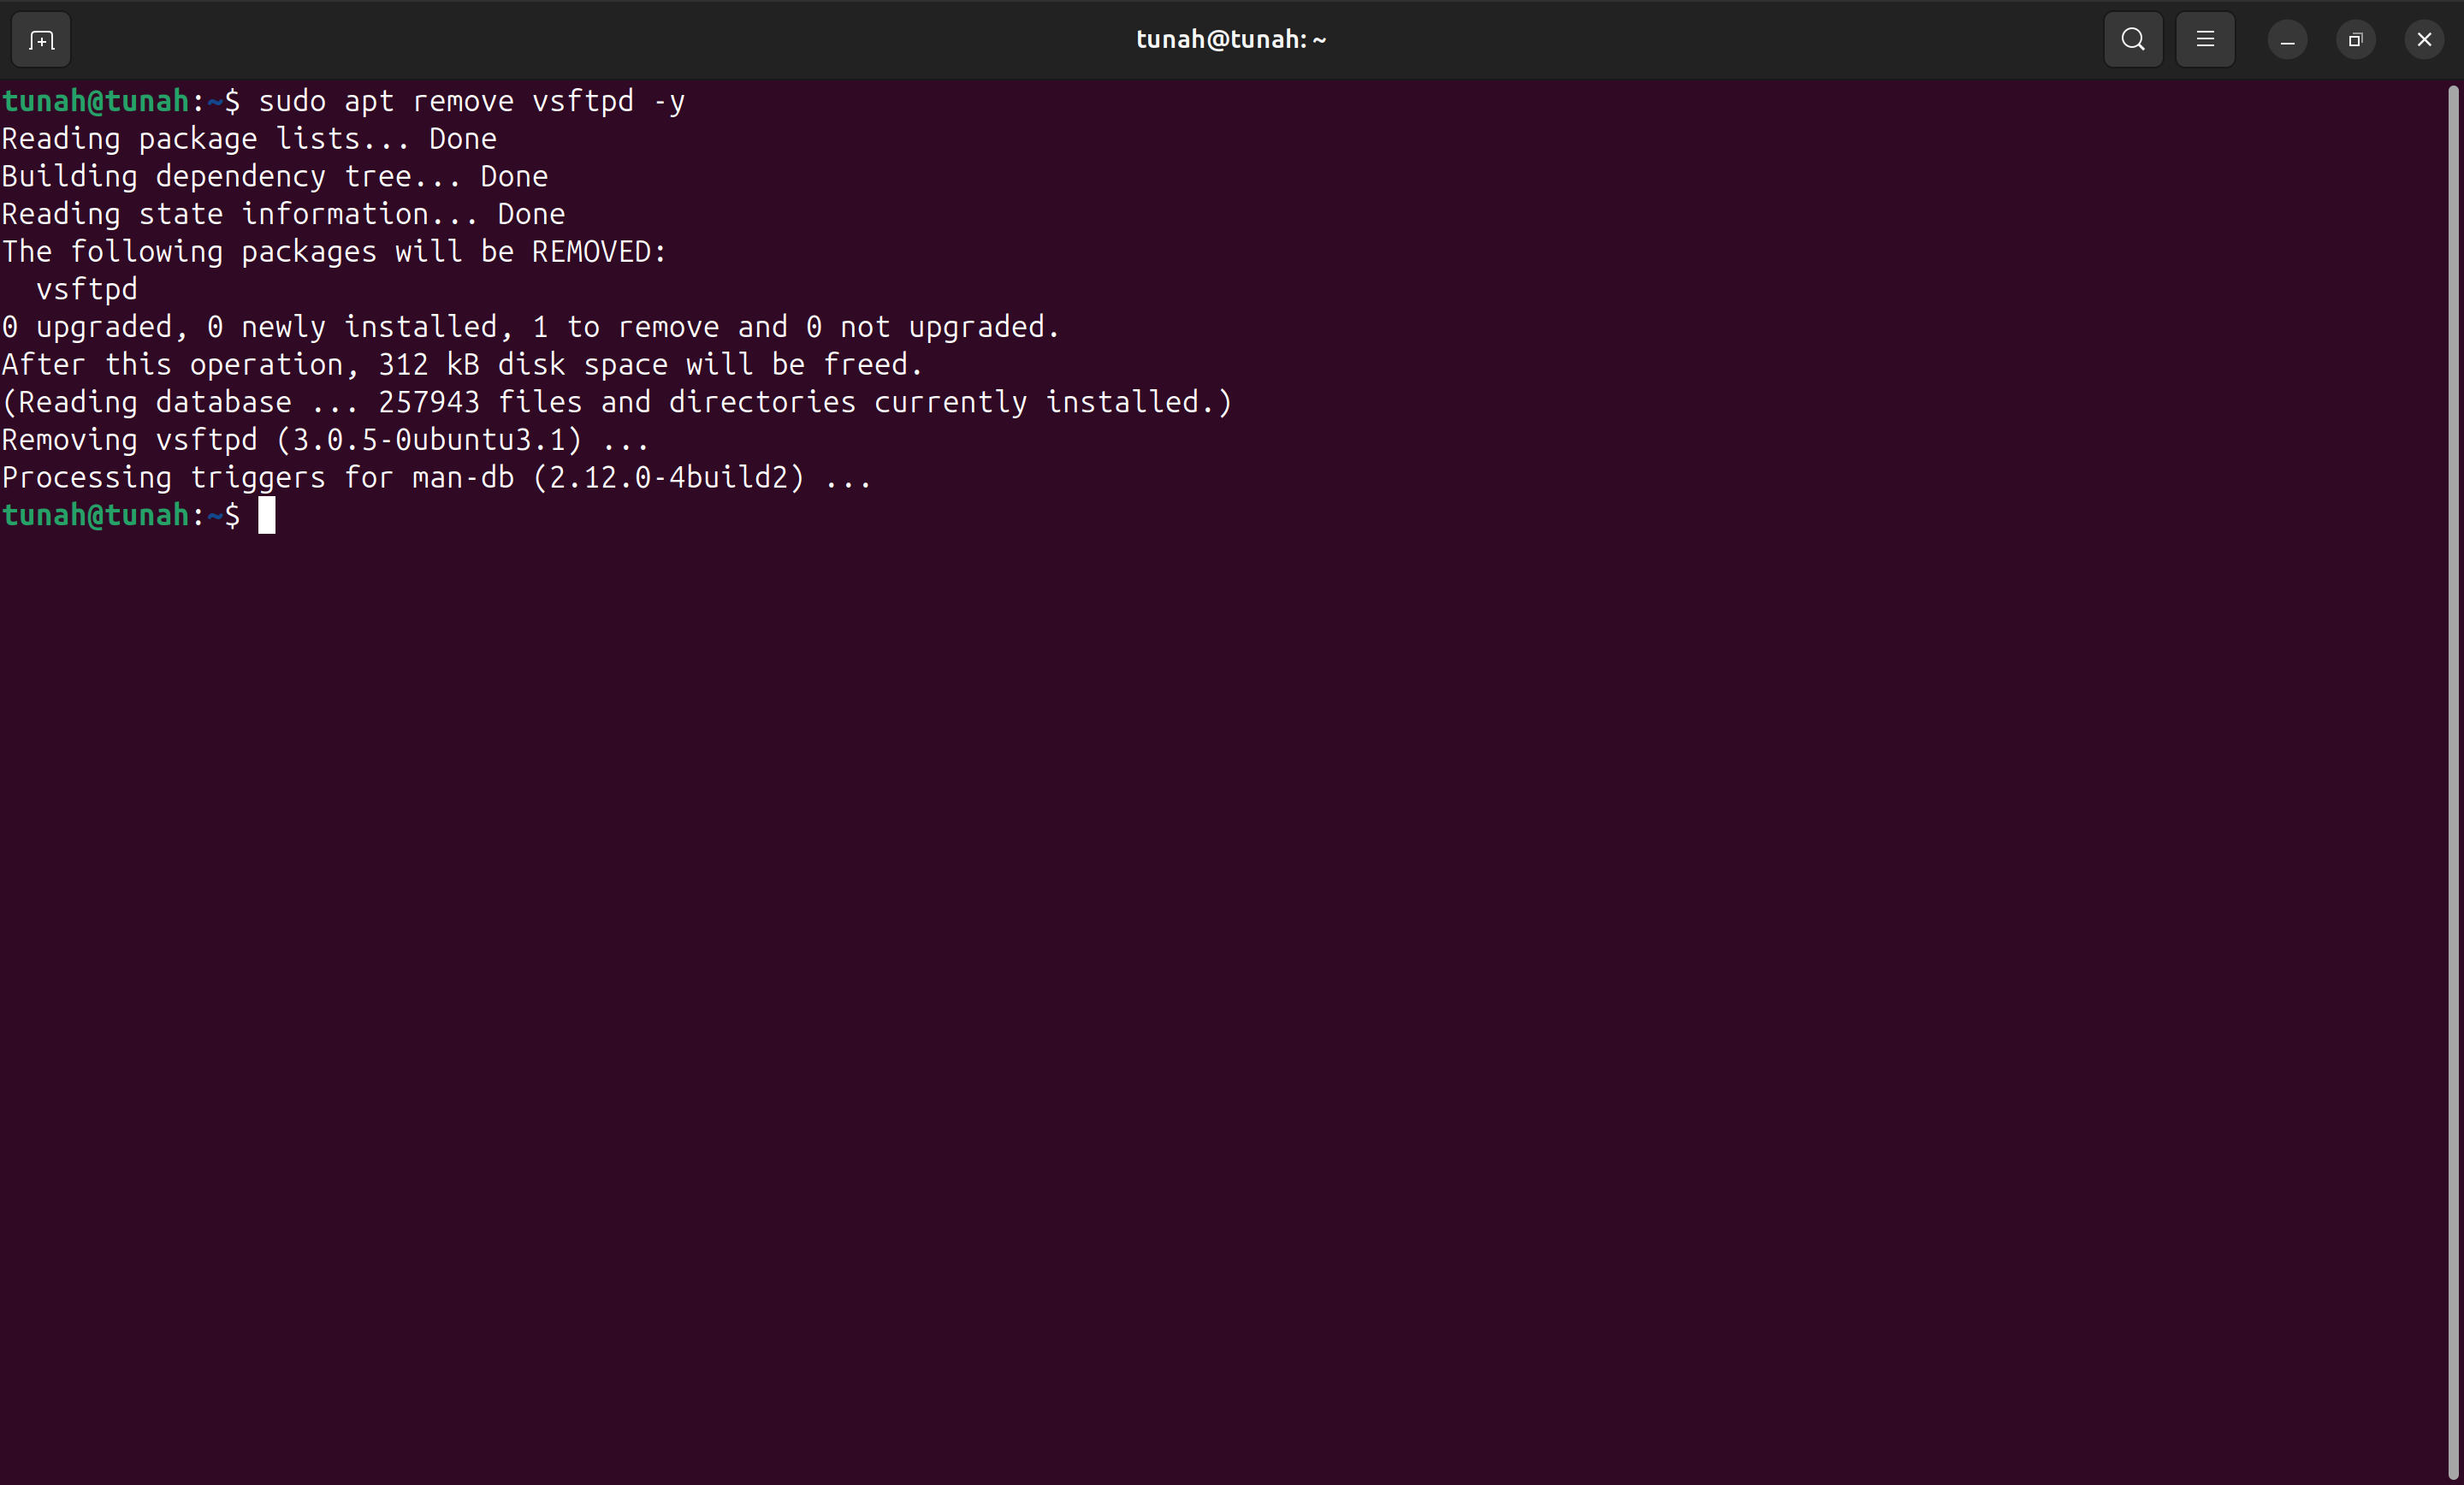
\includegraphics[width=\textwidth]{04/apt-remove-vsftpd.png}
        \caption{Gỡ bỏ vsftpd}
    \end{subfigure}
    \caption{Tra cứu và Gỡ cài đặt}
\end{figure}

\subsection{Quản lý Dependency và Xử lý sự cố}

\textbf{Cách thực hiện:}
- Liệt kê các gói liên quan tới \texttt{python} đã cài trên máy.
- Xem danh sách các gói phụ thuộc (dependencies) của \texttt{vim}.
- Sử dụng \texttt{--fix-broken install} để sửa lỗi package và \texttt{autoremove} để dọn dẹp hệ thống.

\begin{lstlisting}[language=bash]
# Liet ke goi python
dpkg -l | grep python

# Xem phu thuoc cua vim
apt depends vim

# Sua loi va don dep
sudo apt --fix-broken install
sudo apt autoremove -y
\end{lstlisting}

\textbf{Kết quả:}
Quản lý hiệu quả được danh sách các package đã cài và giải phóng không gian ổ cứng an toàn.

\begin{figure}[H]
    \centering
    \begin{subfigure}[b]{0.48\textwidth}
        \centering
        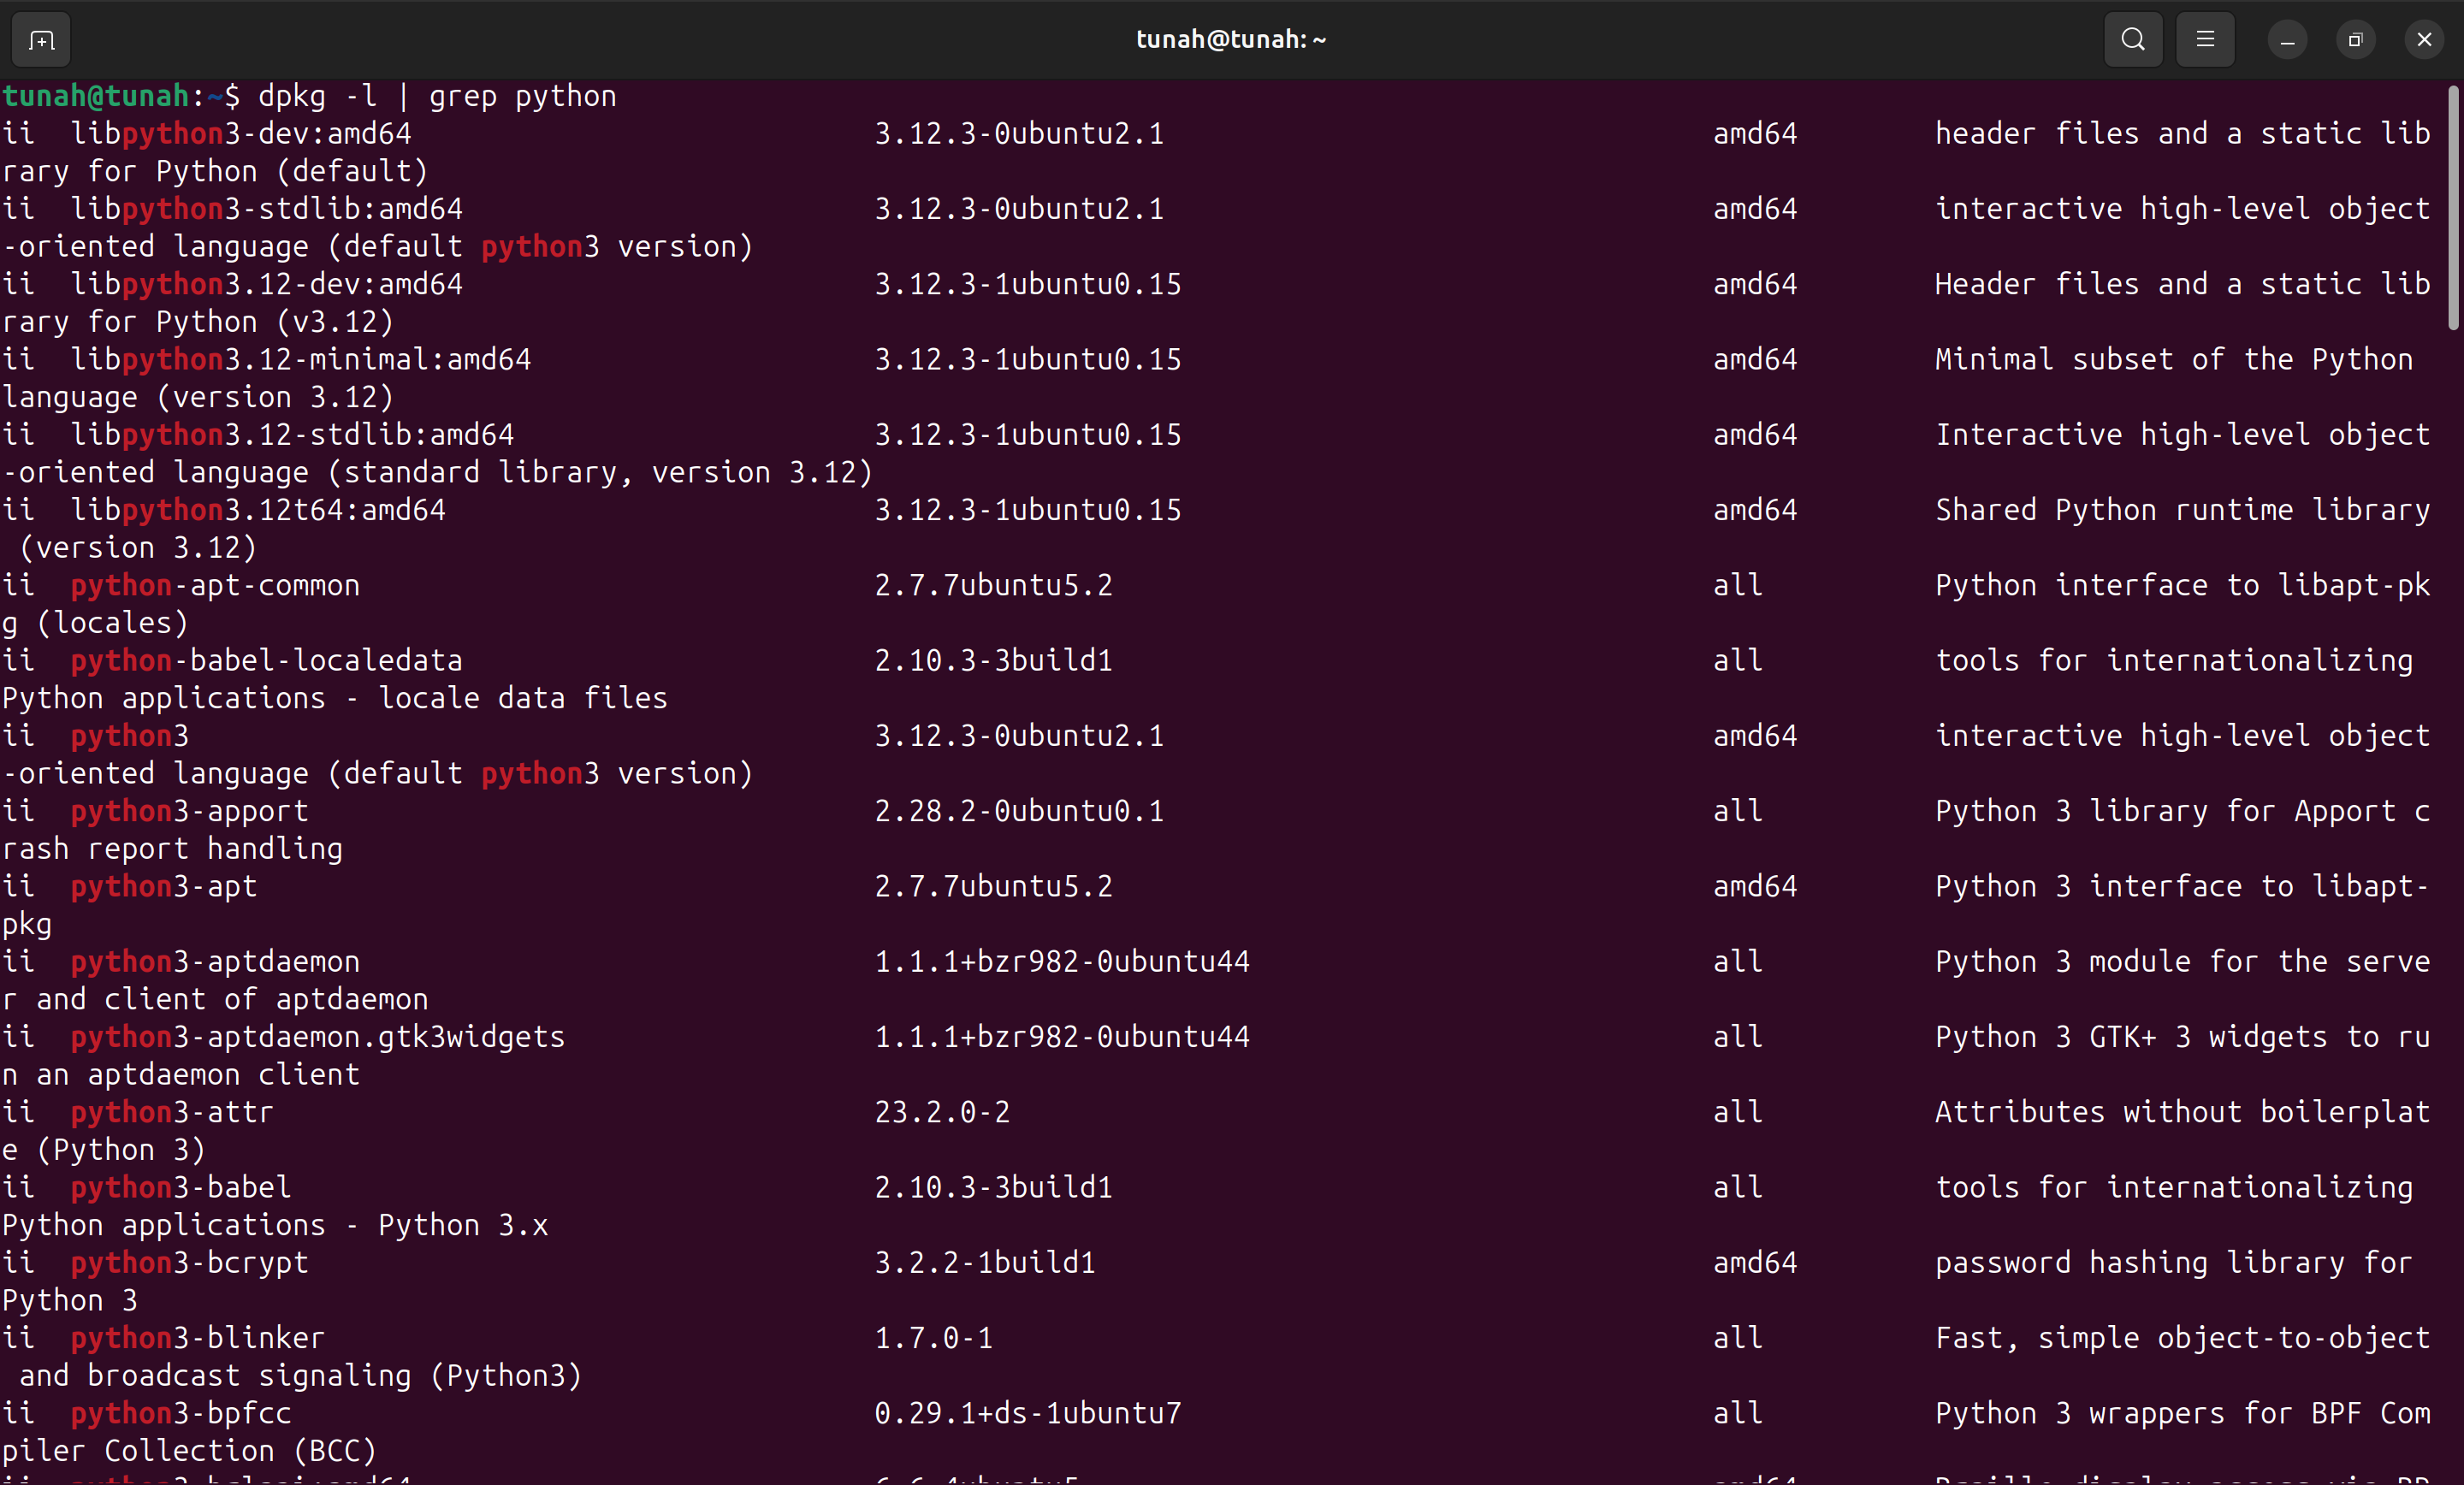
\includegraphics[width=\textwidth]{04/dpkg-grep-python.png}
        \caption{Liệt kê gói cài đặt}
    \end{subfigure}
    \hfill
    \begin{subfigure}[b]{0.48\textwidth}
        \centering
        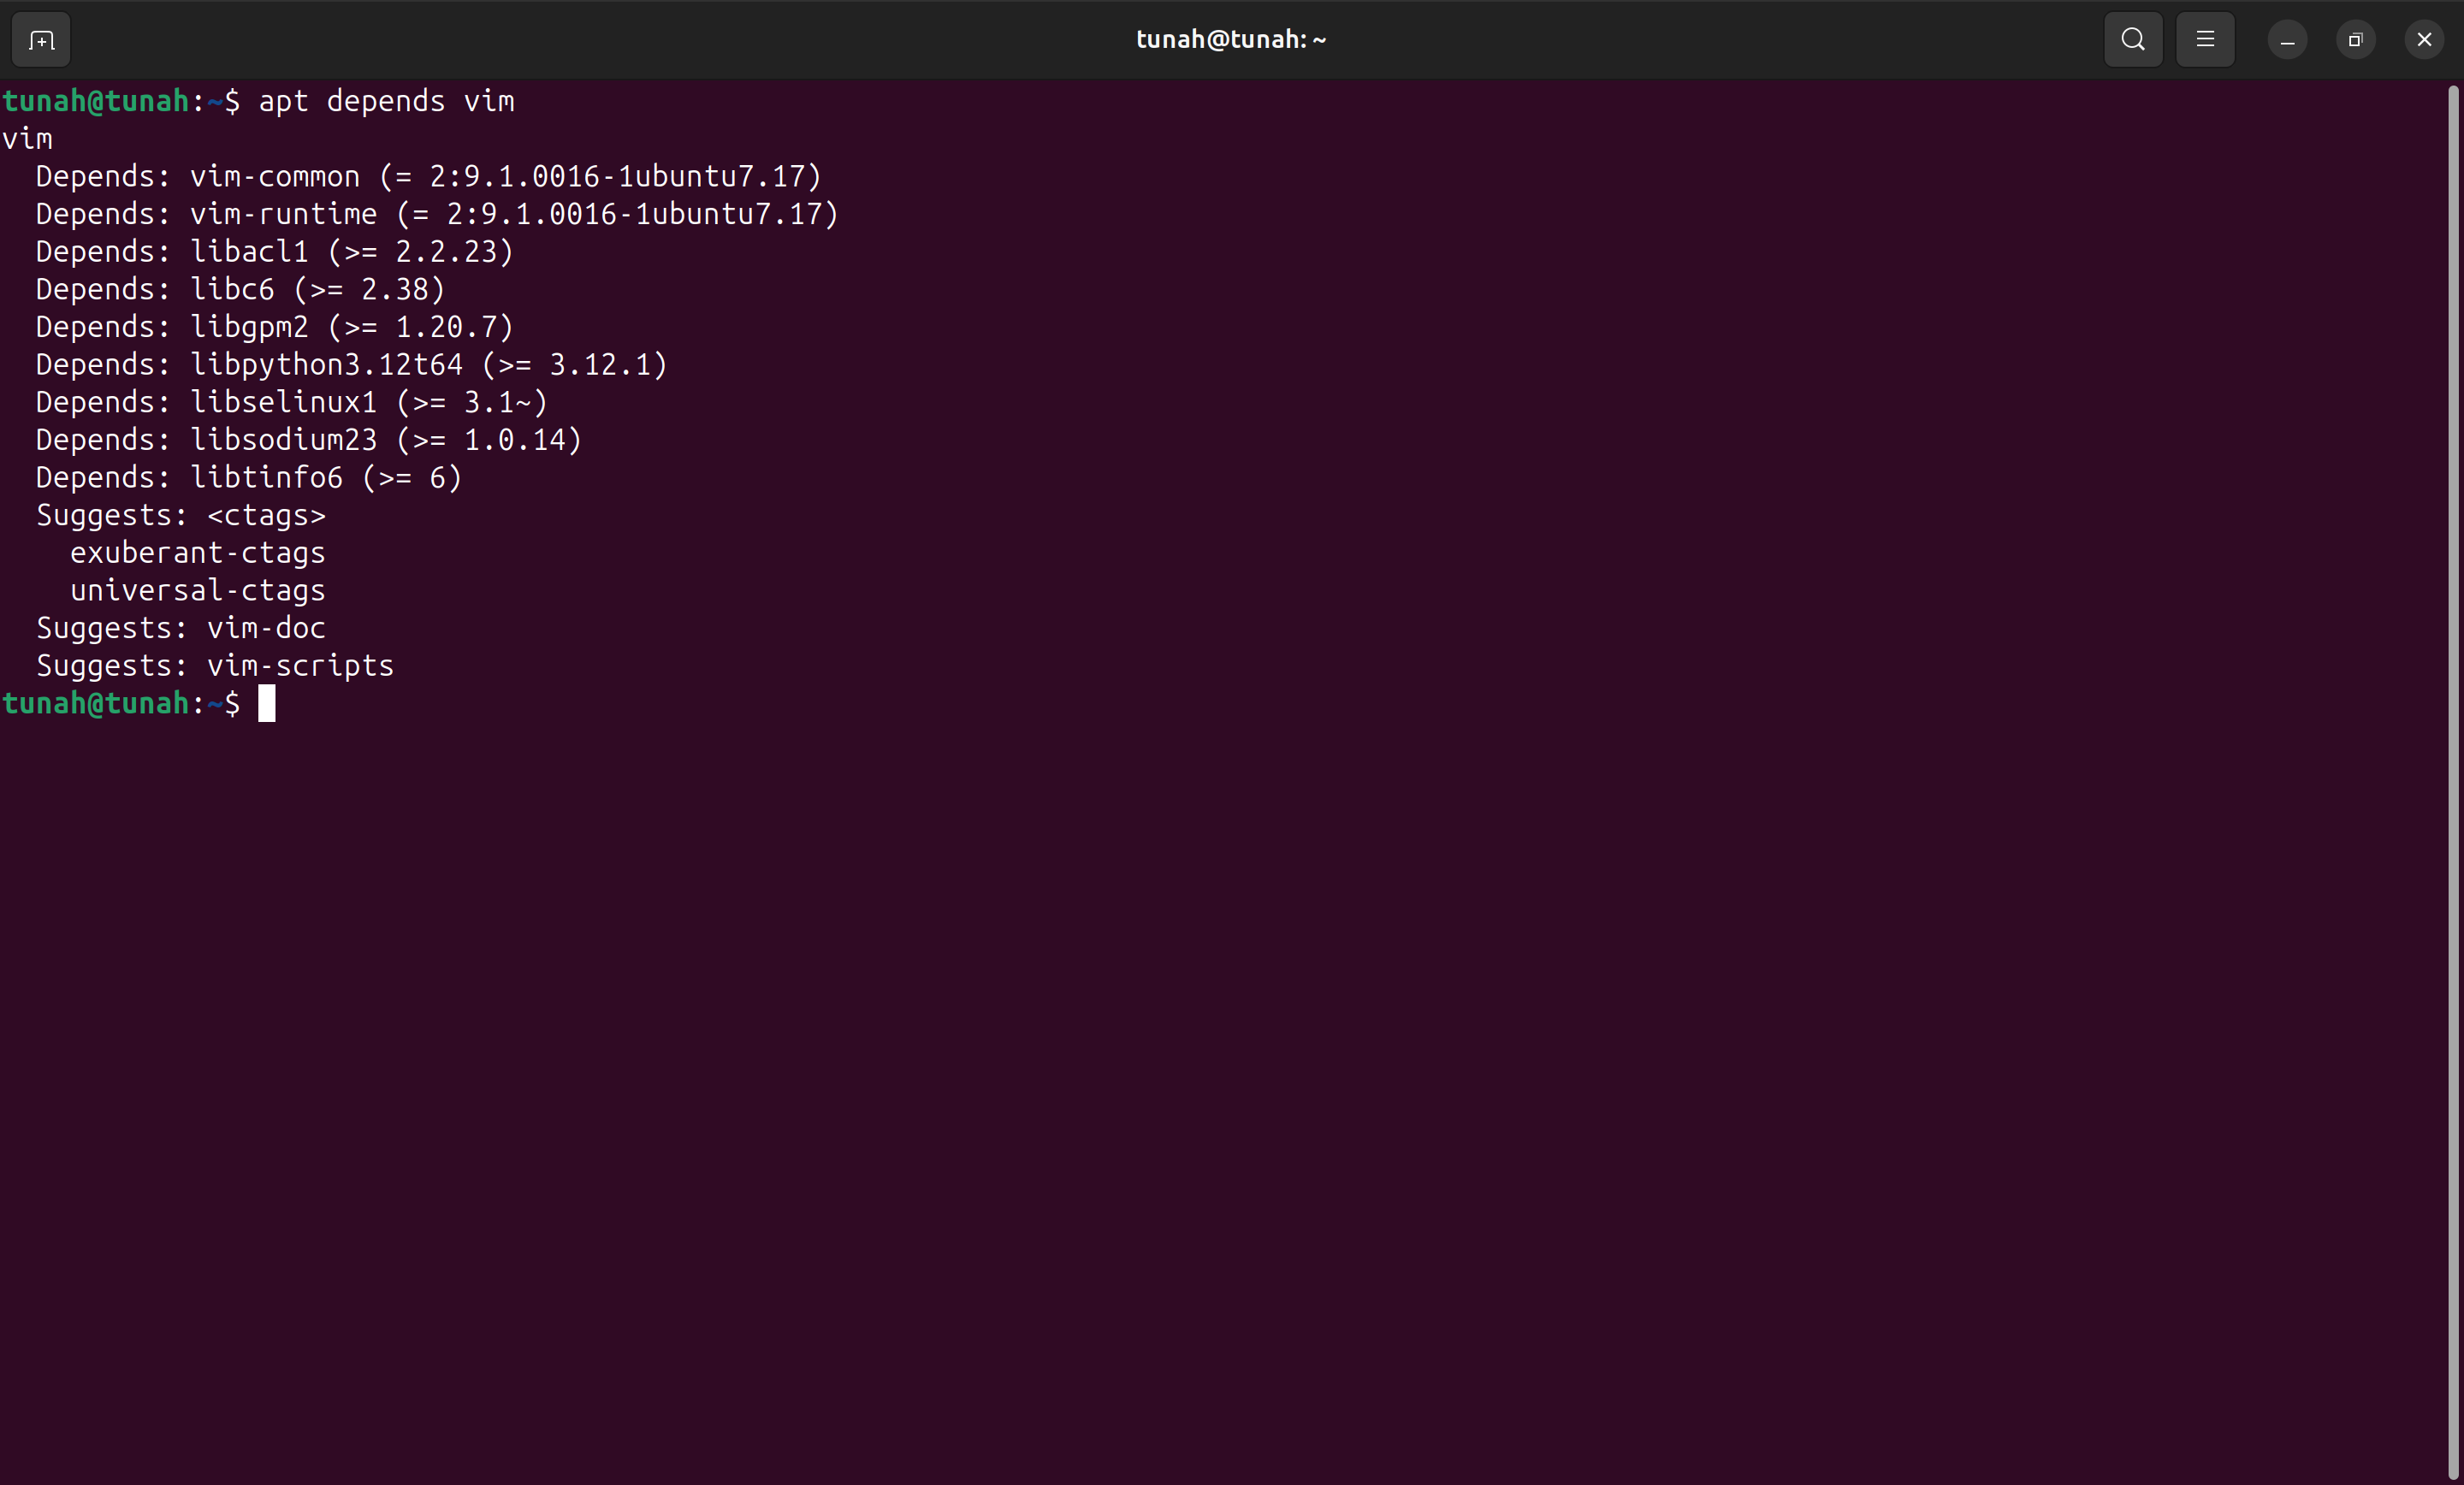
\includegraphics[width=\textwidth]{04/apt-depends-vim.png}
        \caption{Phụ thuộc của vim}
    \end{subfigure}
    
    \vspace{0.5cm}
    \begin{subfigure}[b]{0.48\textwidth}
        \centering
        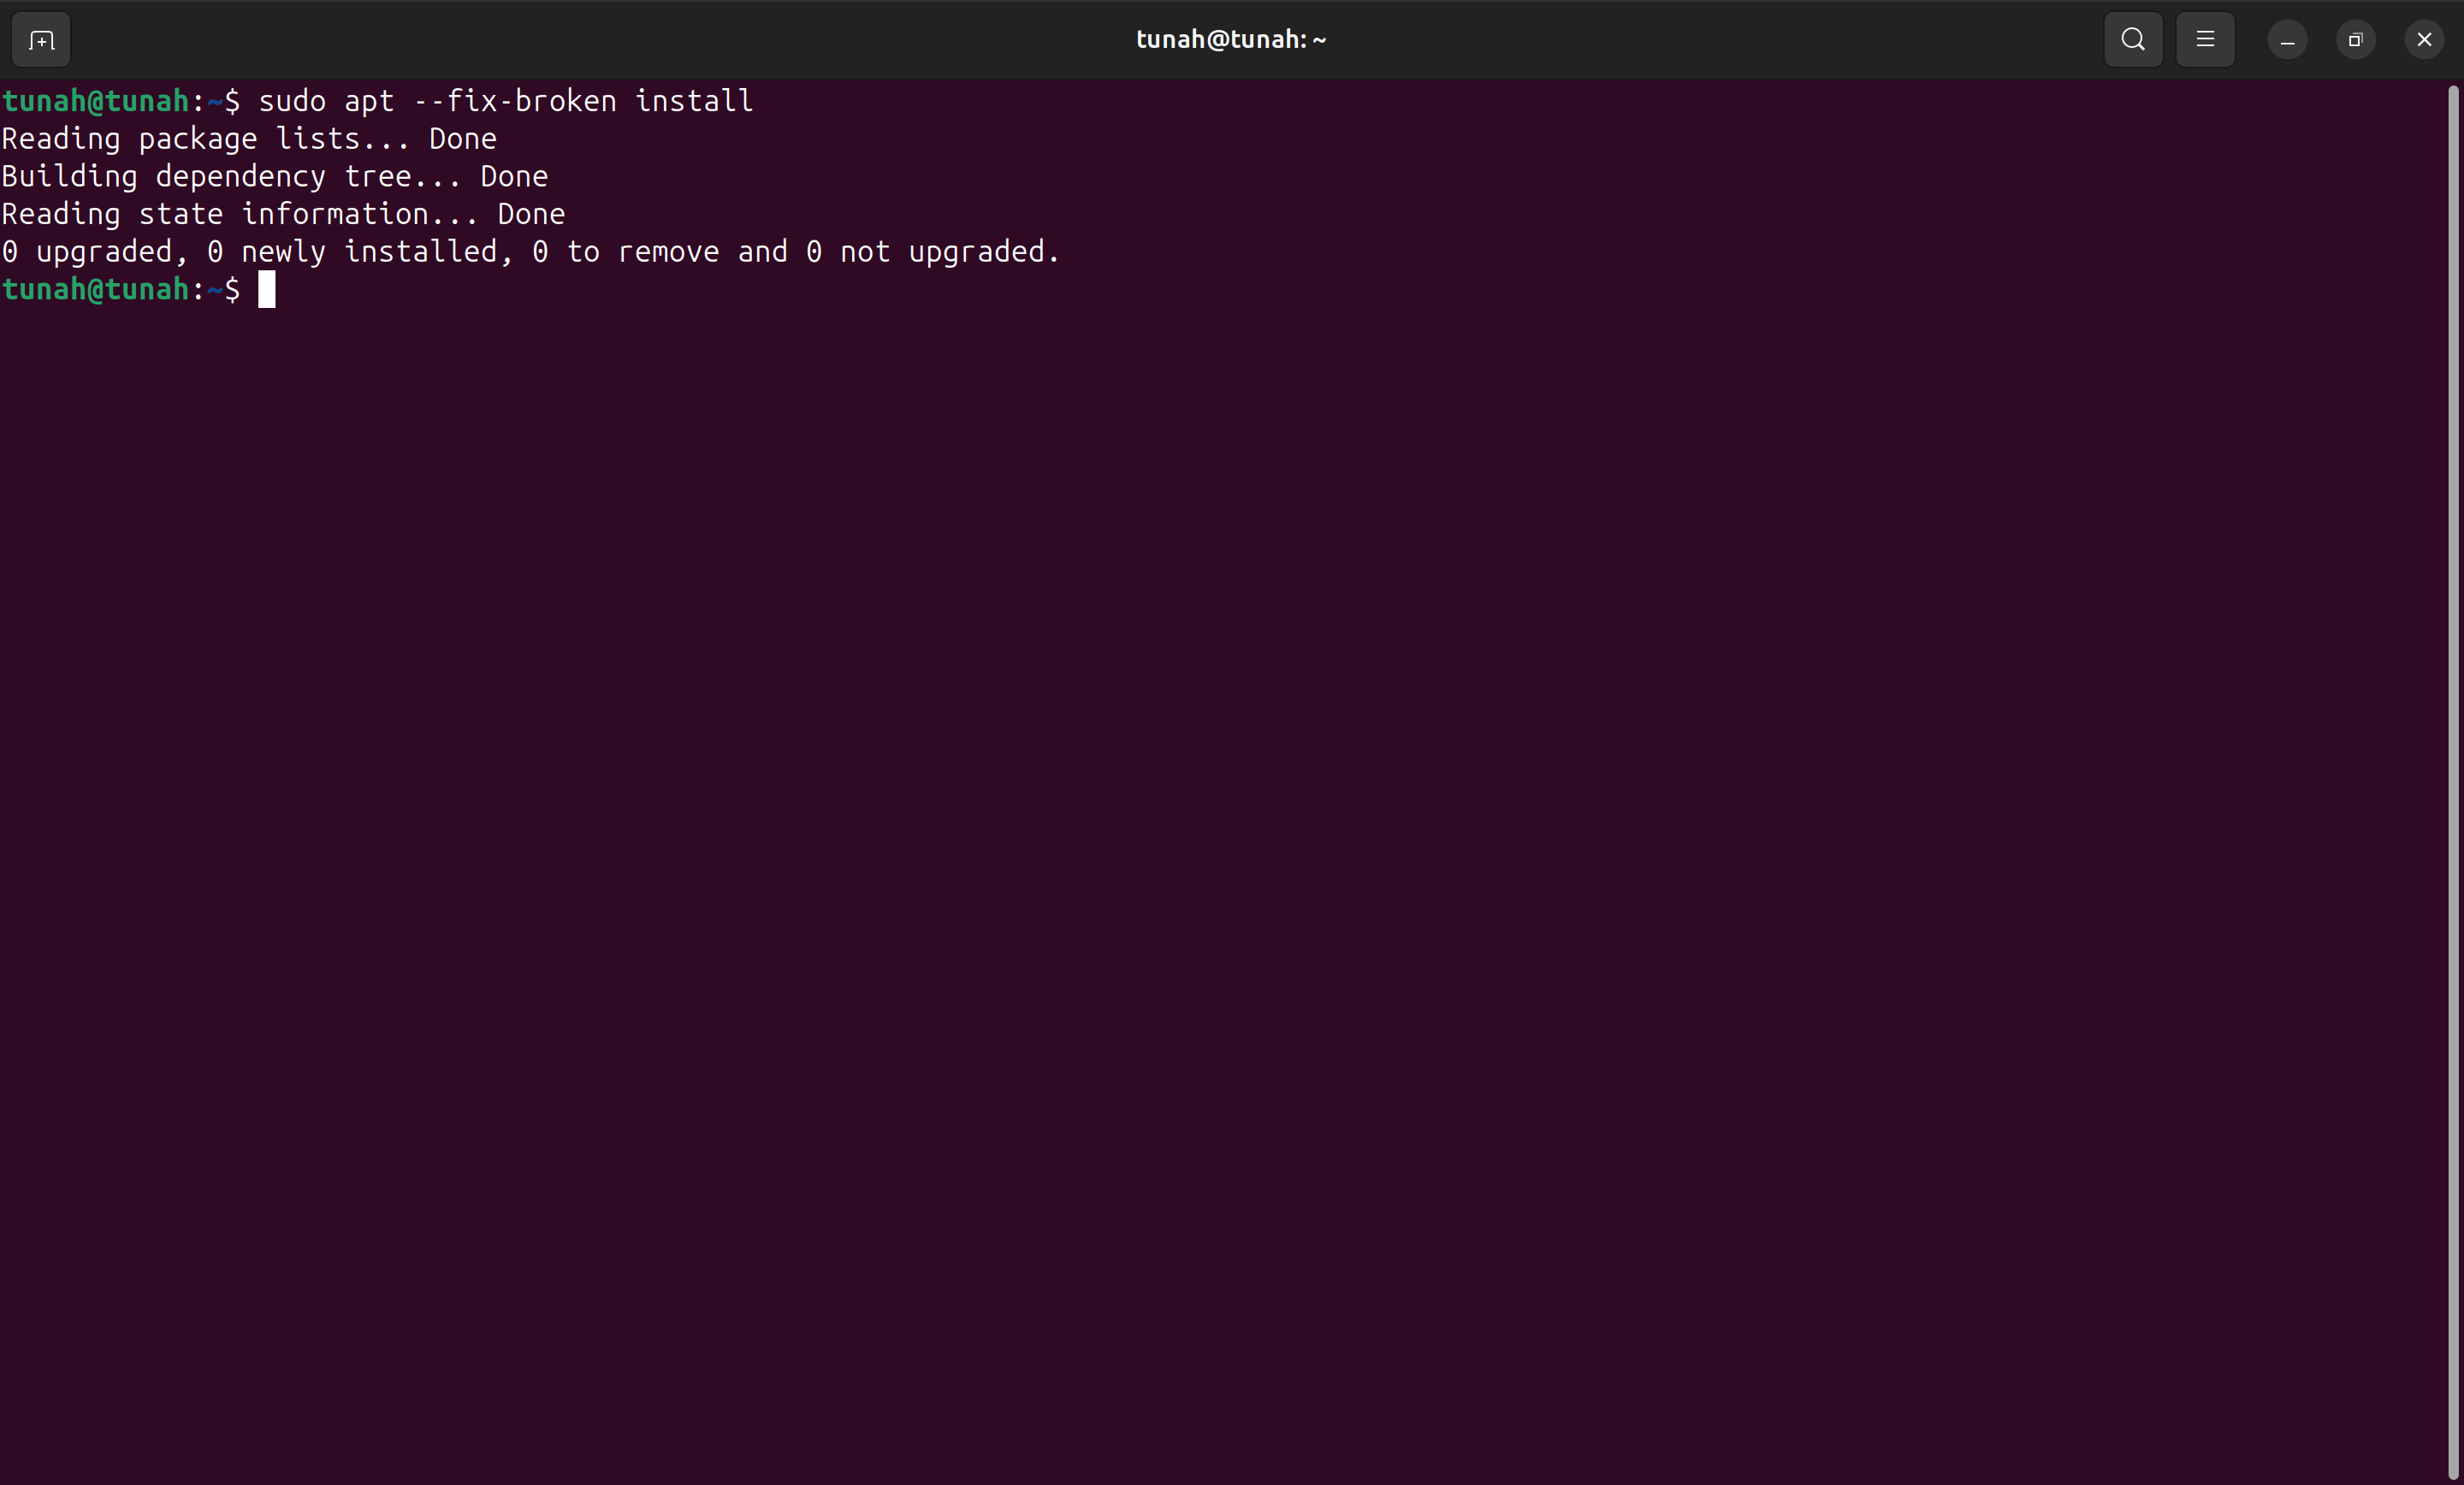
\includegraphics[width=\textwidth]{04/apt-fix-broken.png}
        \caption{Sửa lỗi package}
    \end{subfigure}
    \hfill
    \begin{subfigure}[b]{0.48\textwidth}
        \centering
        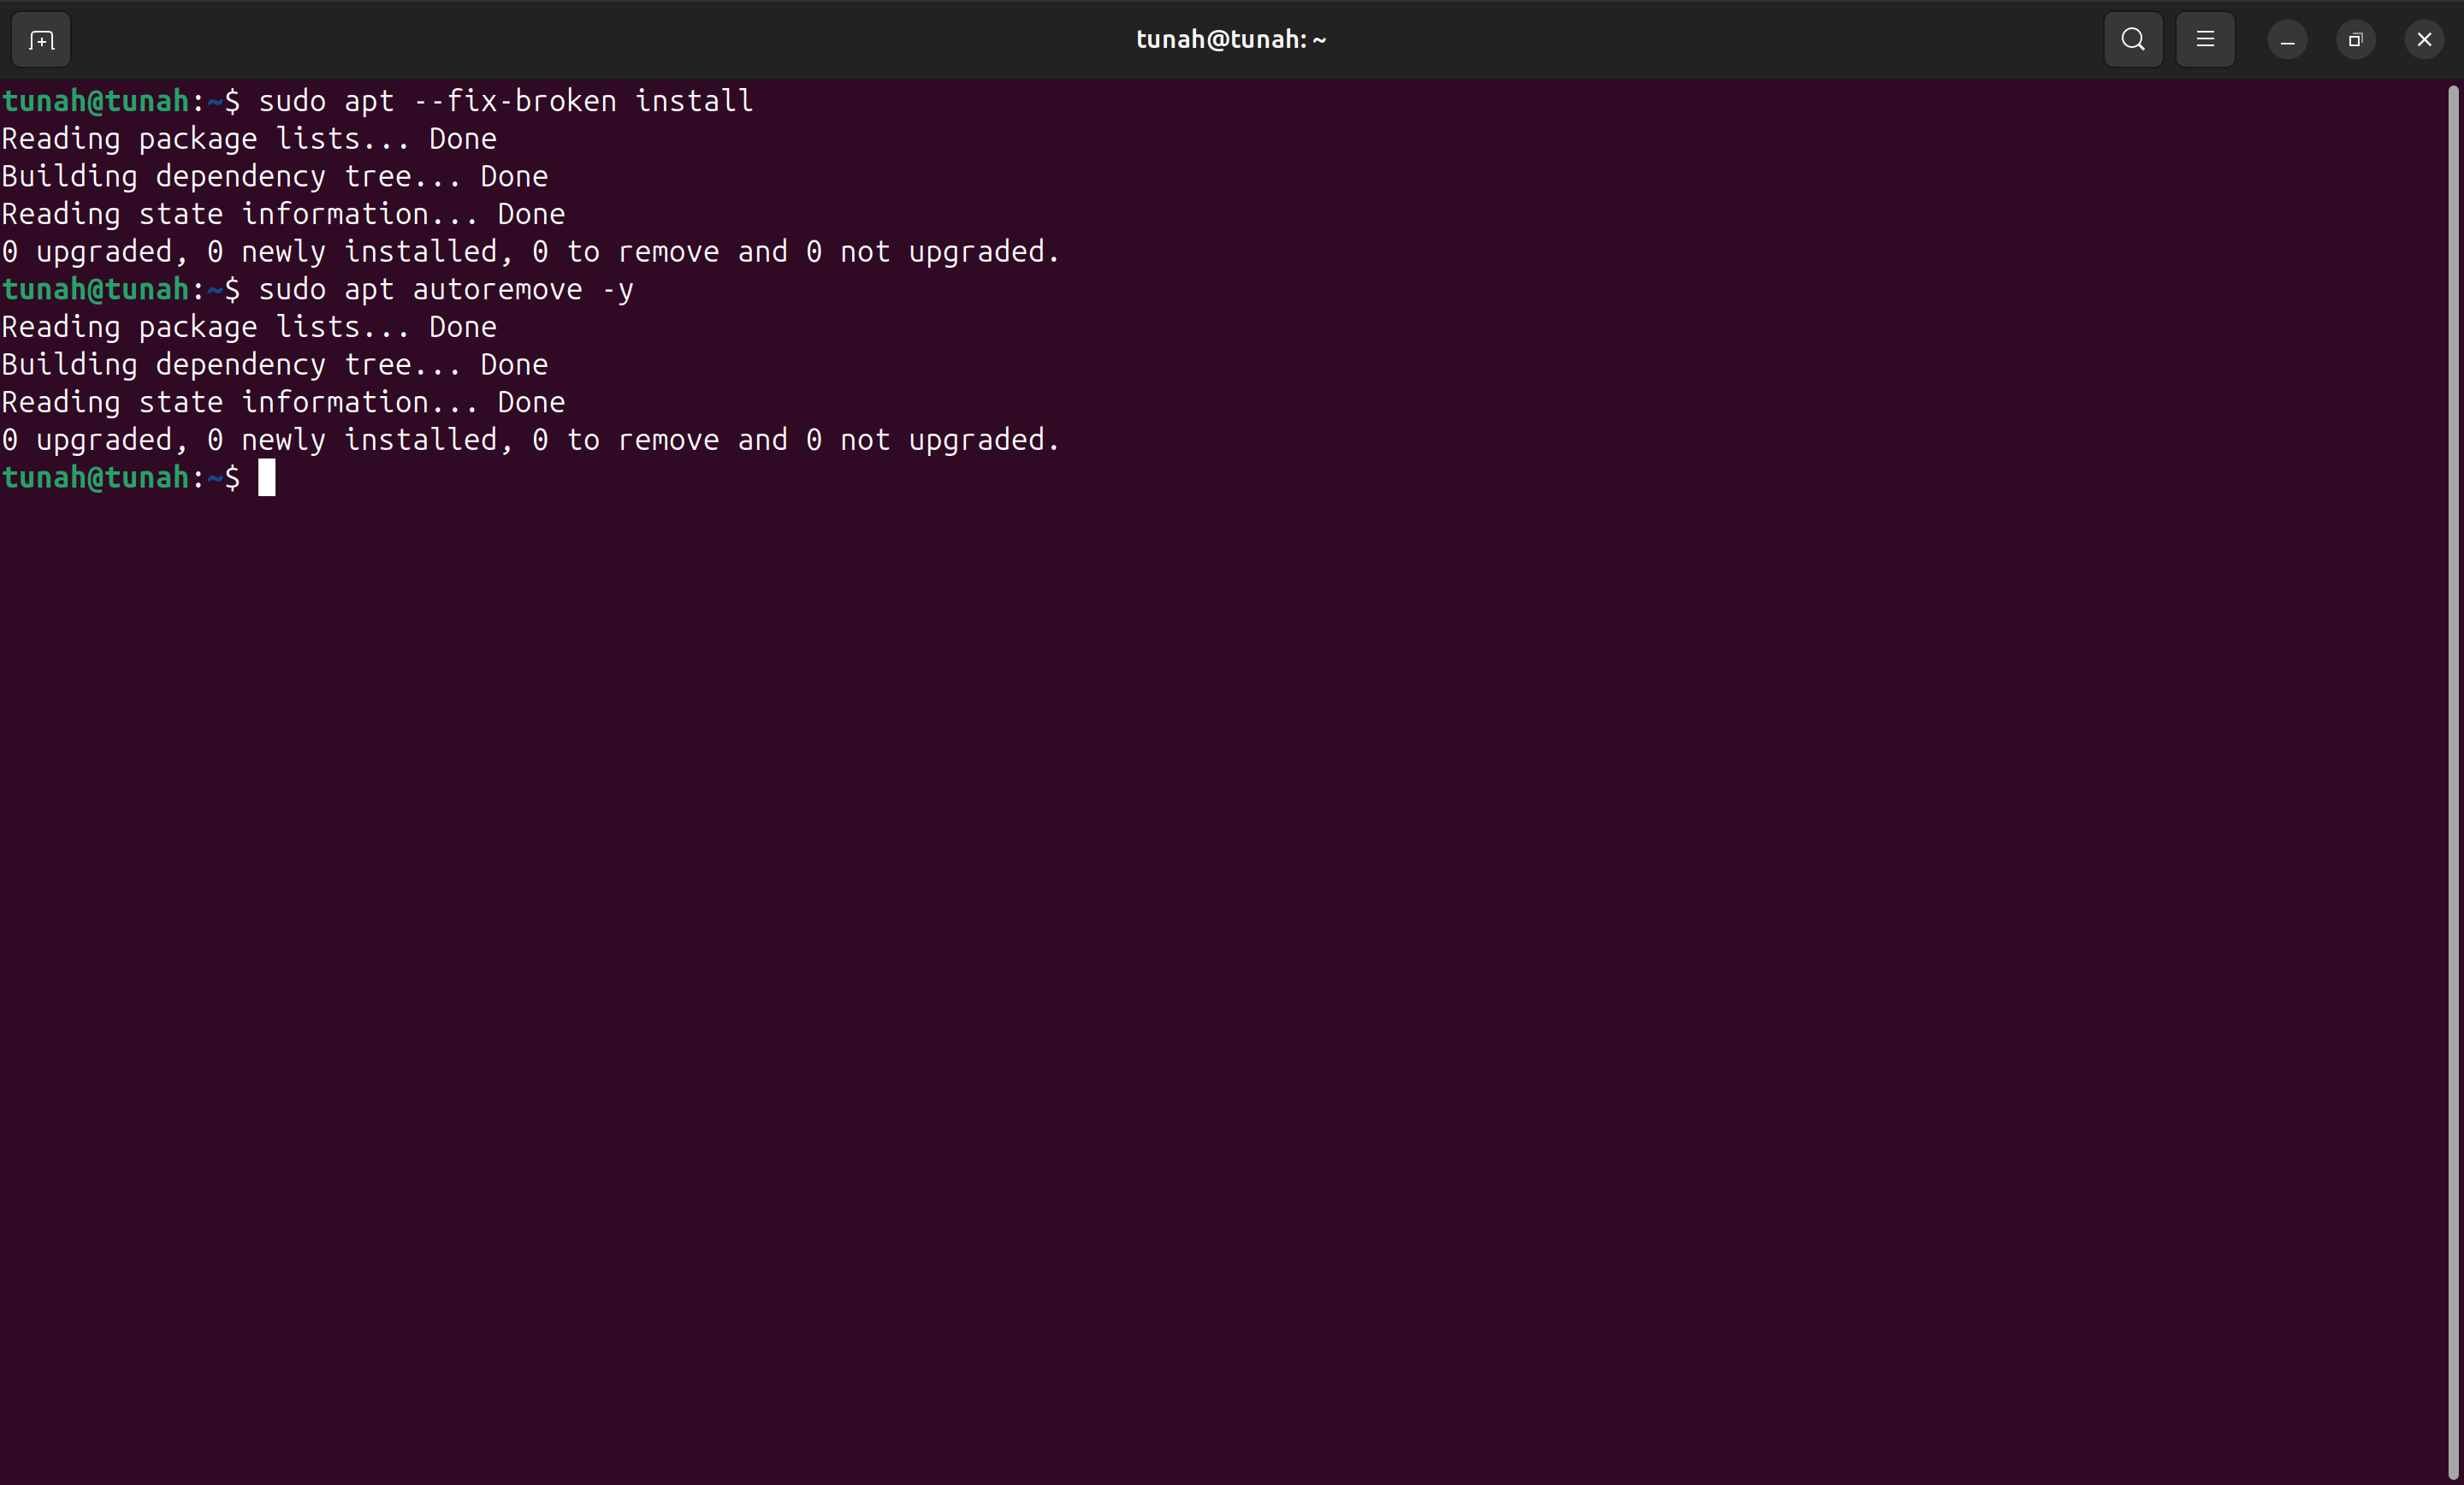
\includegraphics[width=\textwidth]{04/apt-autoremove.png}
        \caption{Lệnh dọn dẹp autoremove}
    \end{subfigure}
    \caption{Bảo trì hệ thống Package}
\end{figure}

\section{Quản lý Dịch vụ (Service Management)}

\subsection{Cài đặt và Quản lý Trạng thái Nginx}

\textbf{Cách thực hiện:}
Cài đặt \texttt{nginx}. Sau đó, sử dụng lệnh \texttt{systemctl} để lần lượt kiểm tra trạng thái, khởi động và dừng dịch vụ web server này.

\begin{lstlisting}[language=bash]
# Cai dat nginx
sudo apt install nginx -y

# Xem trang thai, khoi dong, dung dich vu
sudo systemctl status nginx
sudo systemctl start nginx
sudo systemctl stop nginx
\end{lstlisting}

\textbf{Kết quả:}
Dịch vụ được cài đặt thành công, chuyển đổi trạng thái giữa \texttt{active (running)} và \texttt{inactive (dead)} ổn định qua \texttt{systemctl}.

\begin{figure}[H]
    \centering
    \begin{subfigure}[b]{0.45\textwidth}
        \centering
        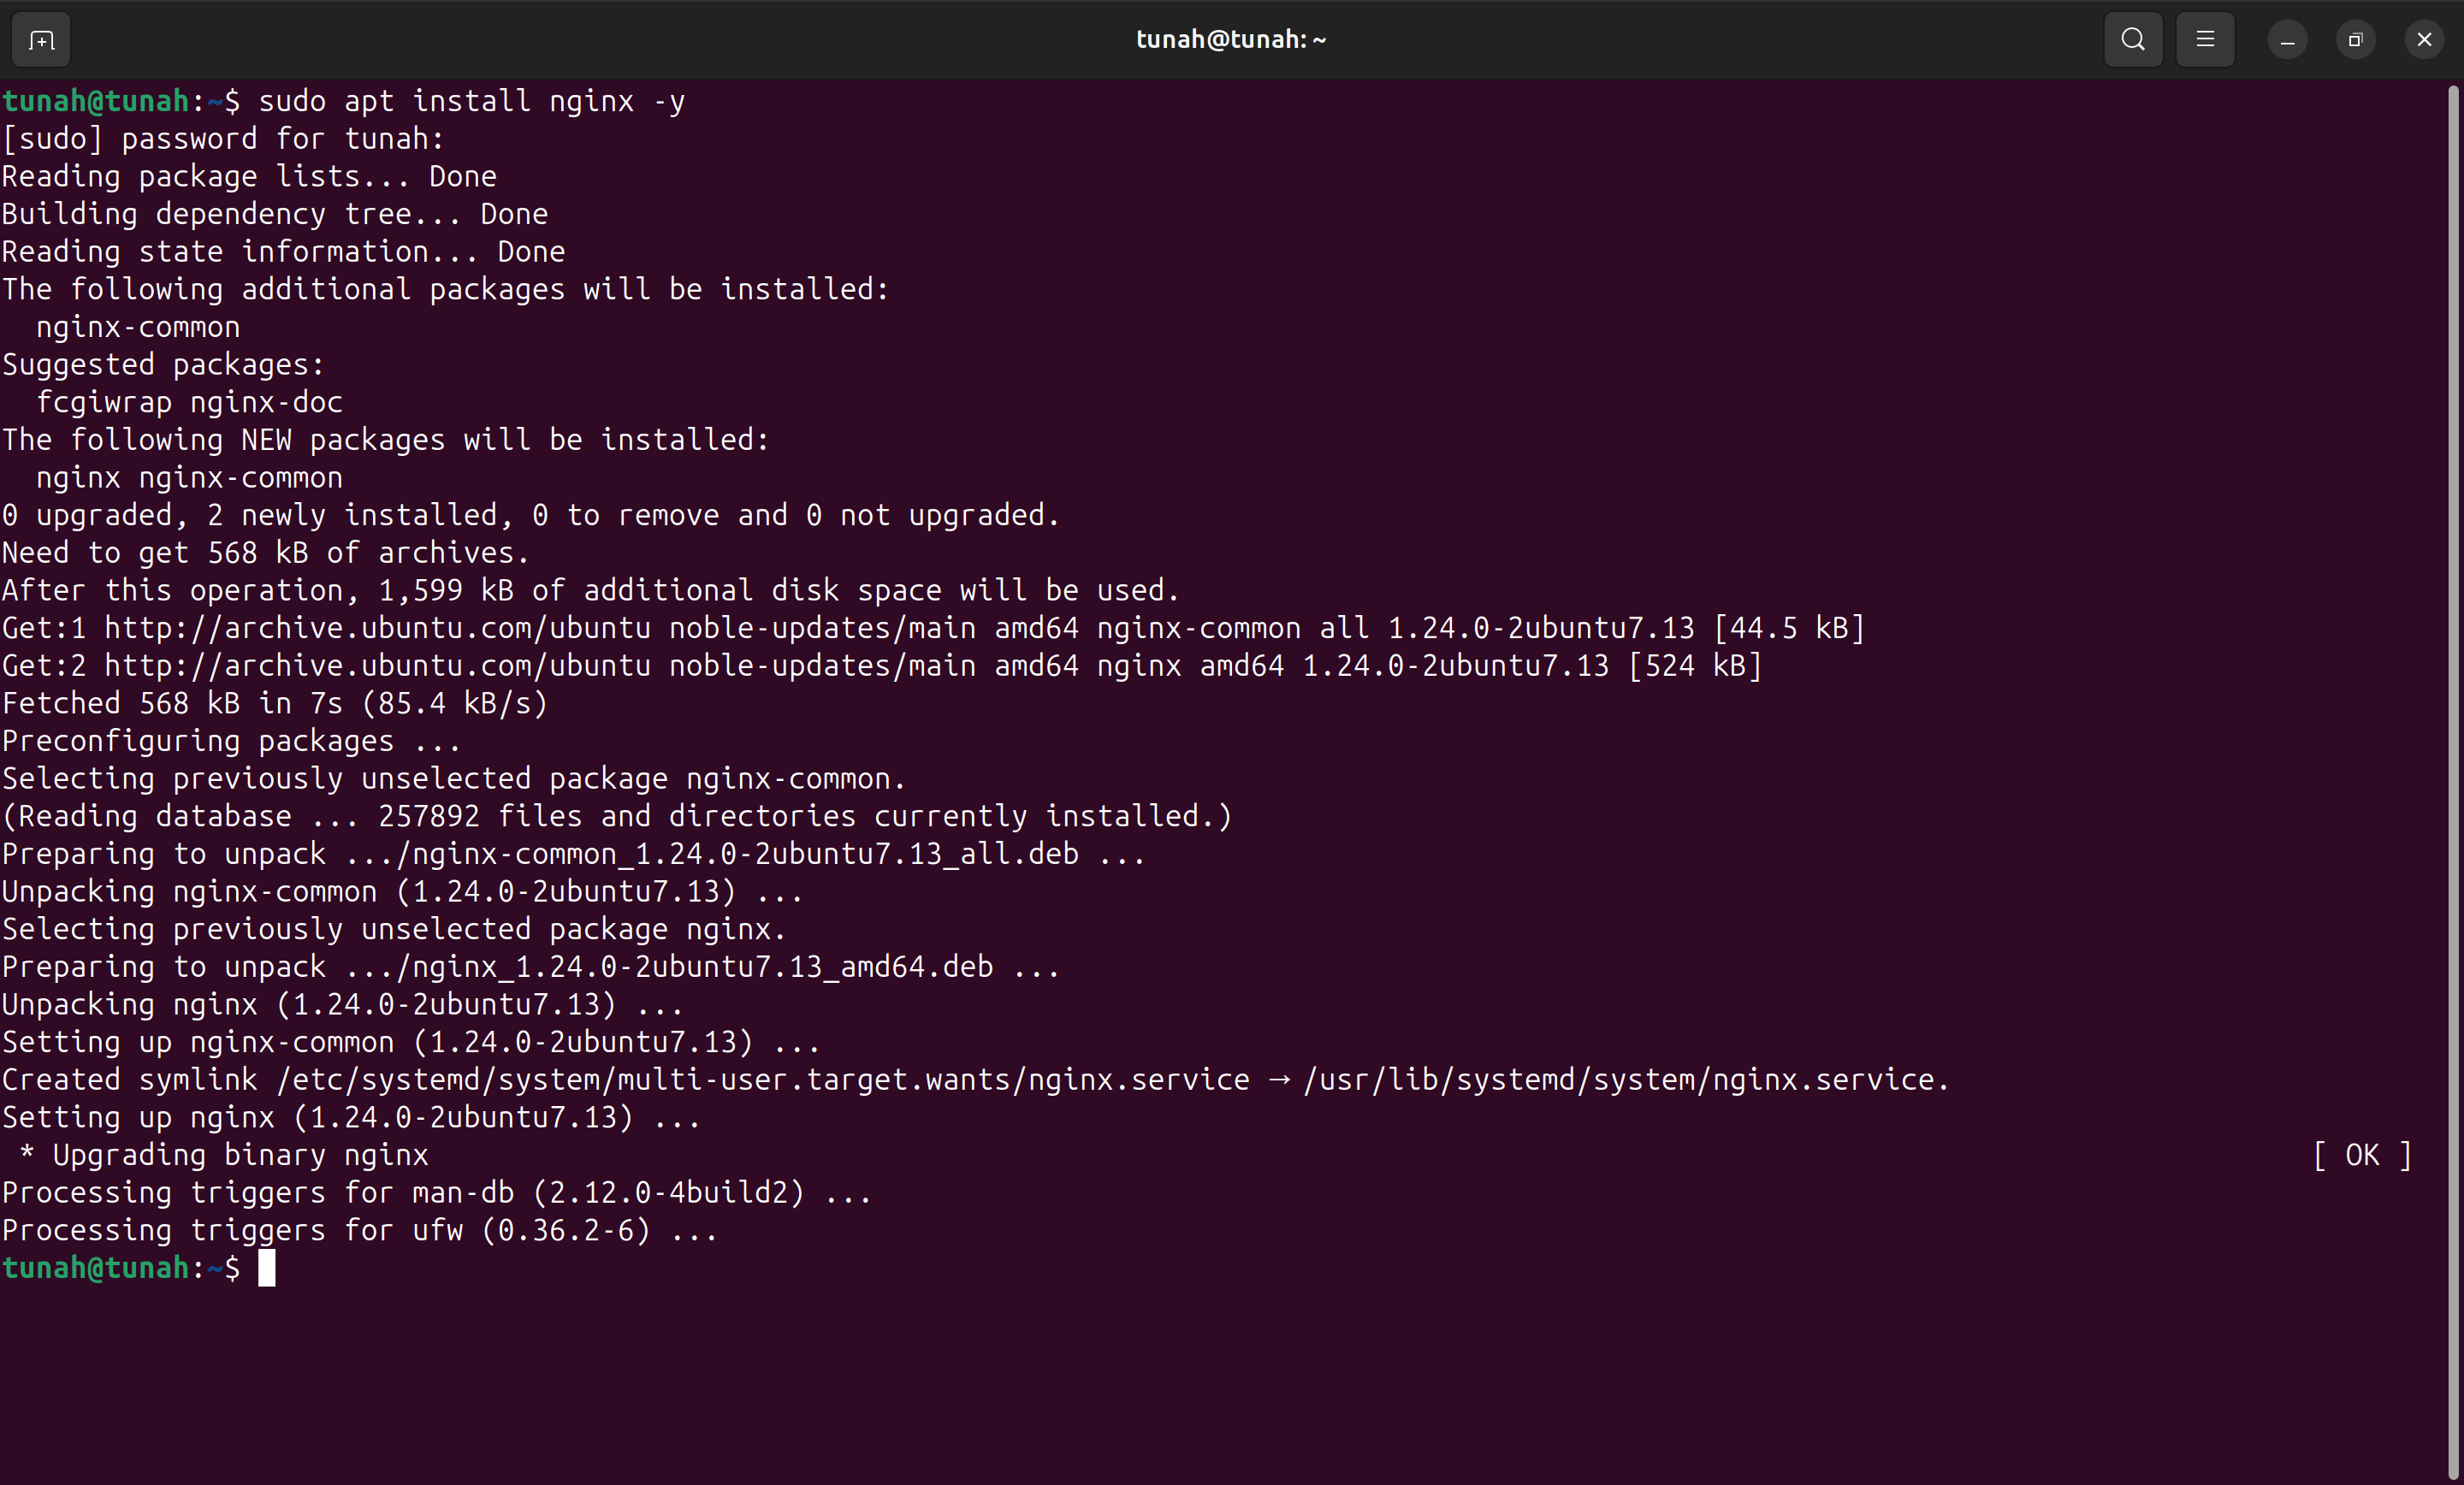
\includegraphics[width=\textwidth]{05/install-nginx.png}
        \caption{Cài đặt nginx}
    \end{subfigure}
    \hfill
    \begin{subfigure}[b]{0.45\textwidth}
        \centering
        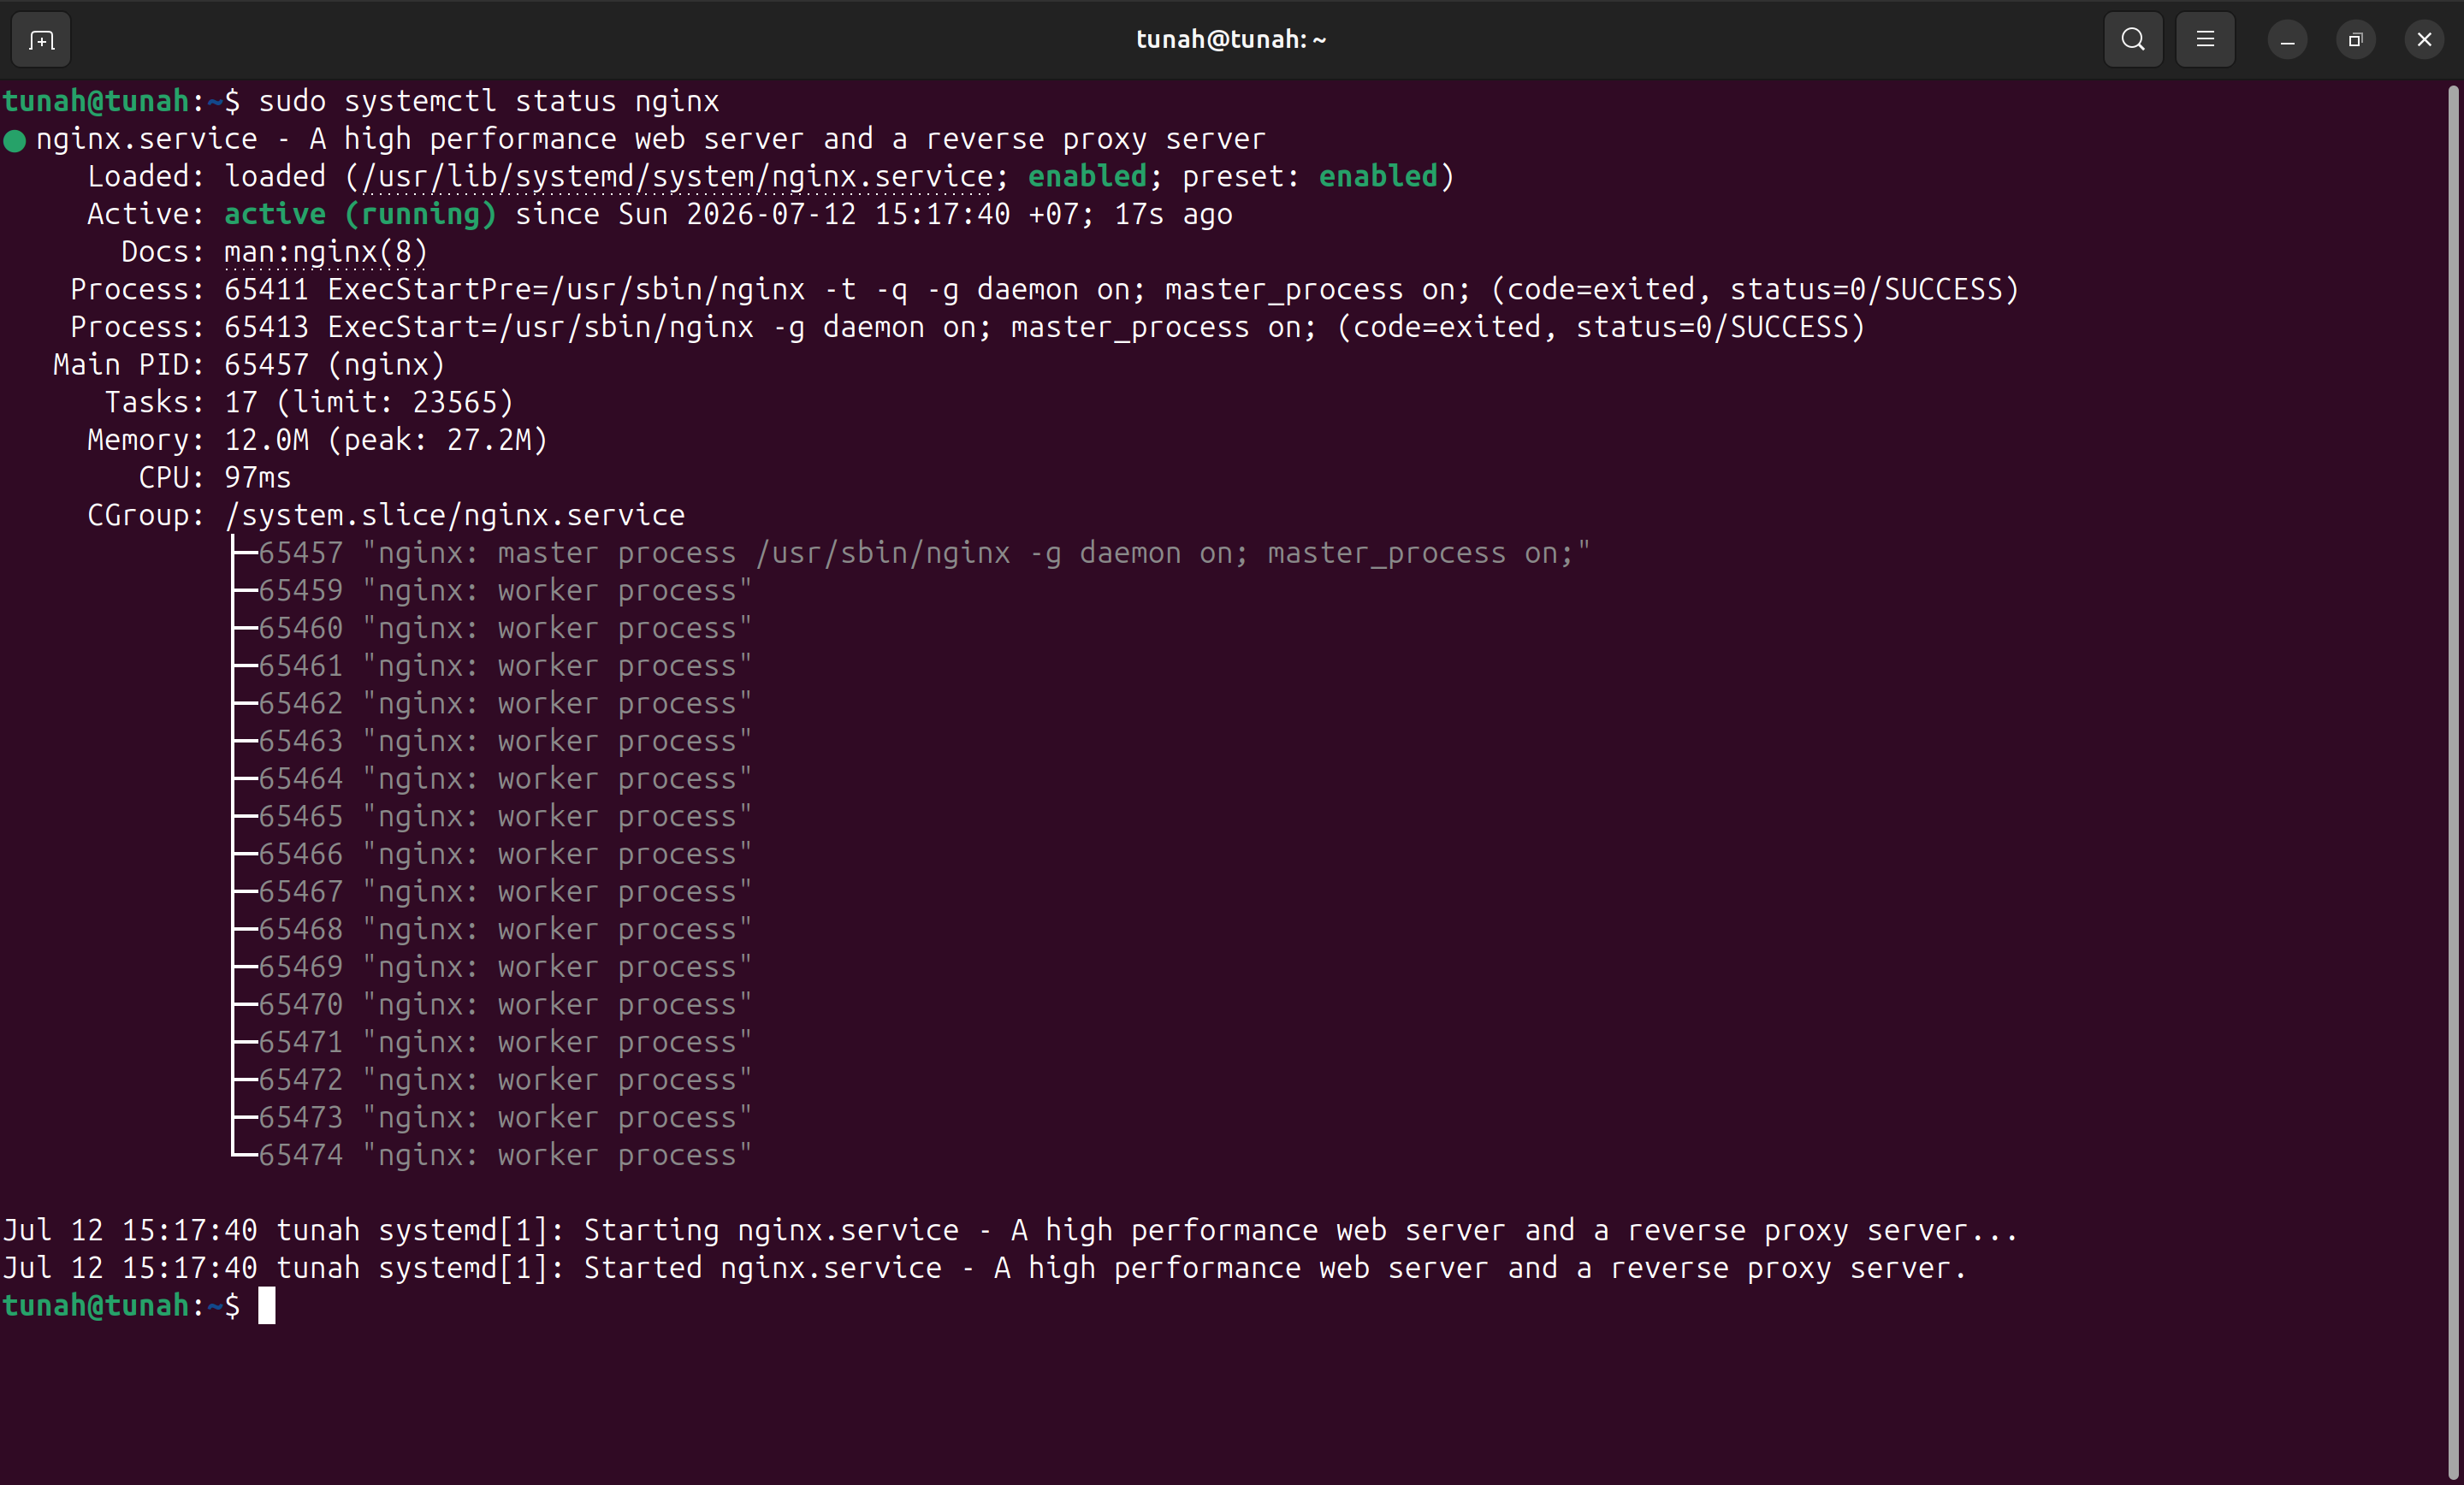
\includegraphics[width=\textwidth]{05/nginx-status-initial.png}
        \caption{Trạng thái ban đầu}
    \end{subfigure}
    
    \vspace{0.5cm}
    \begin{subfigure}[b]{0.45\textwidth}
        \centering
        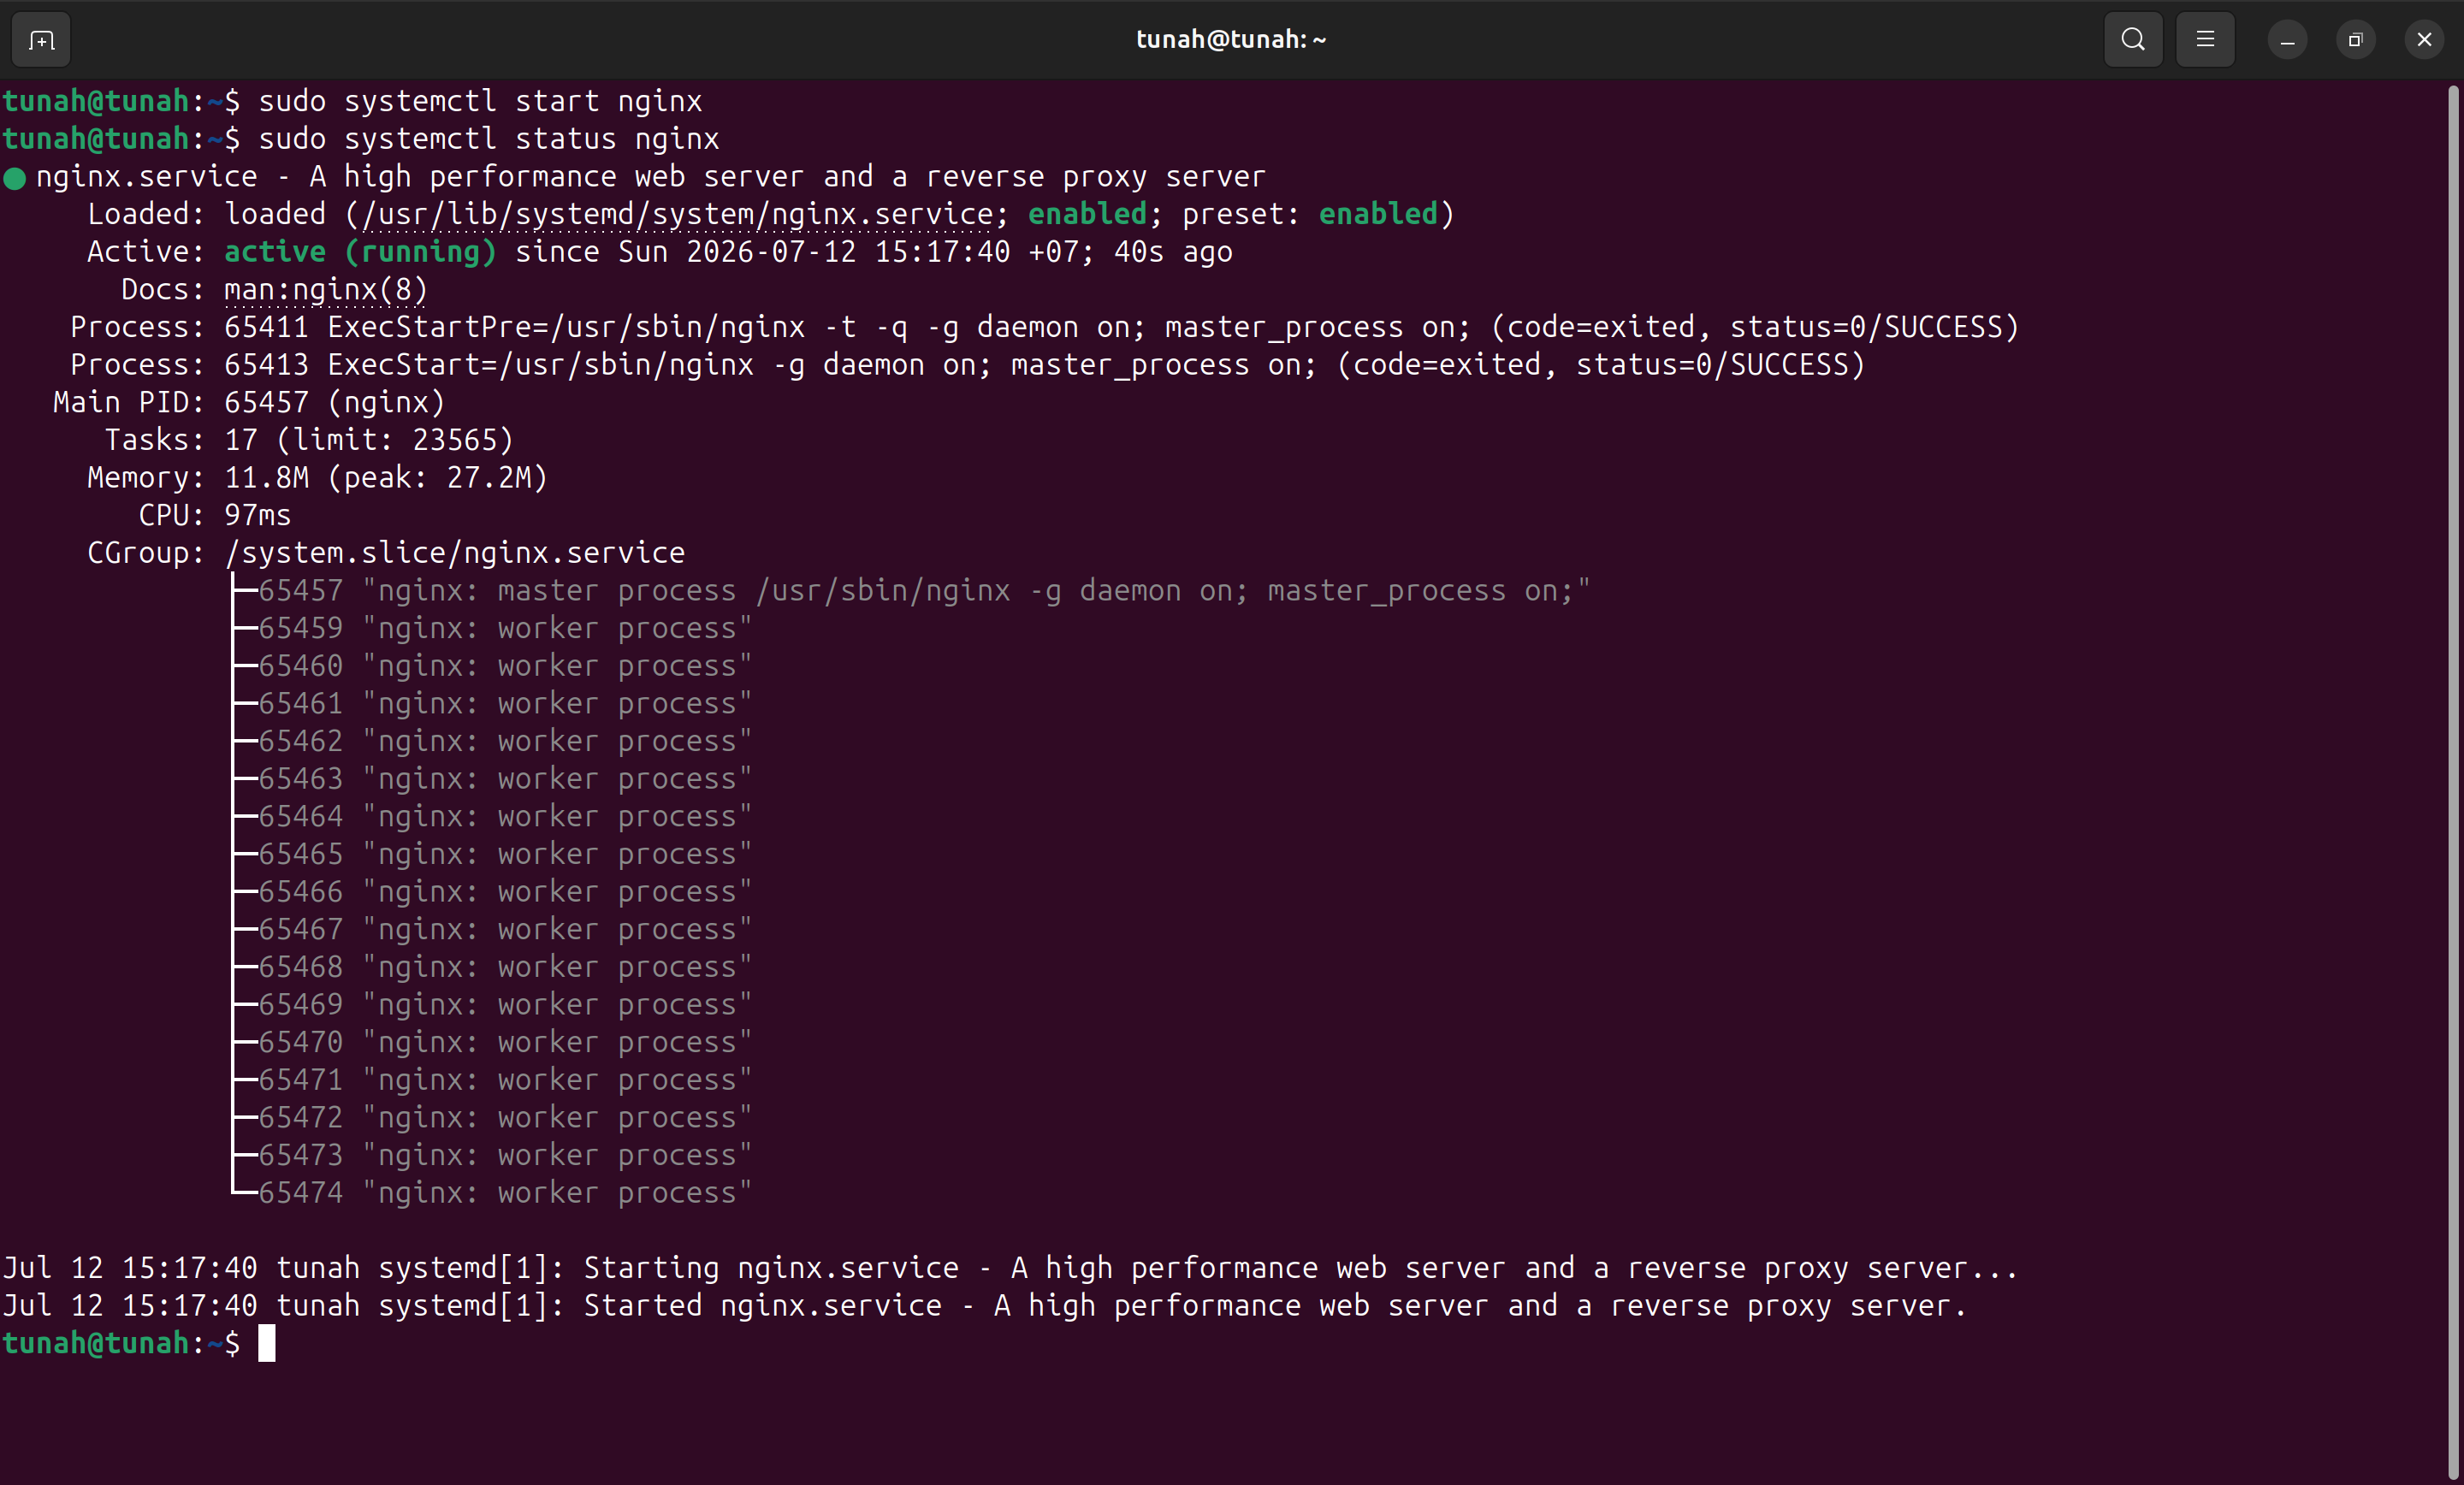
\includegraphics[width=\textwidth]{05/nginx-started.png}
        \caption{Nginx active}
    \end{subfigure}
    \hfill
    \begin{subfigure}[b]{0.45\textwidth}
        \centering
        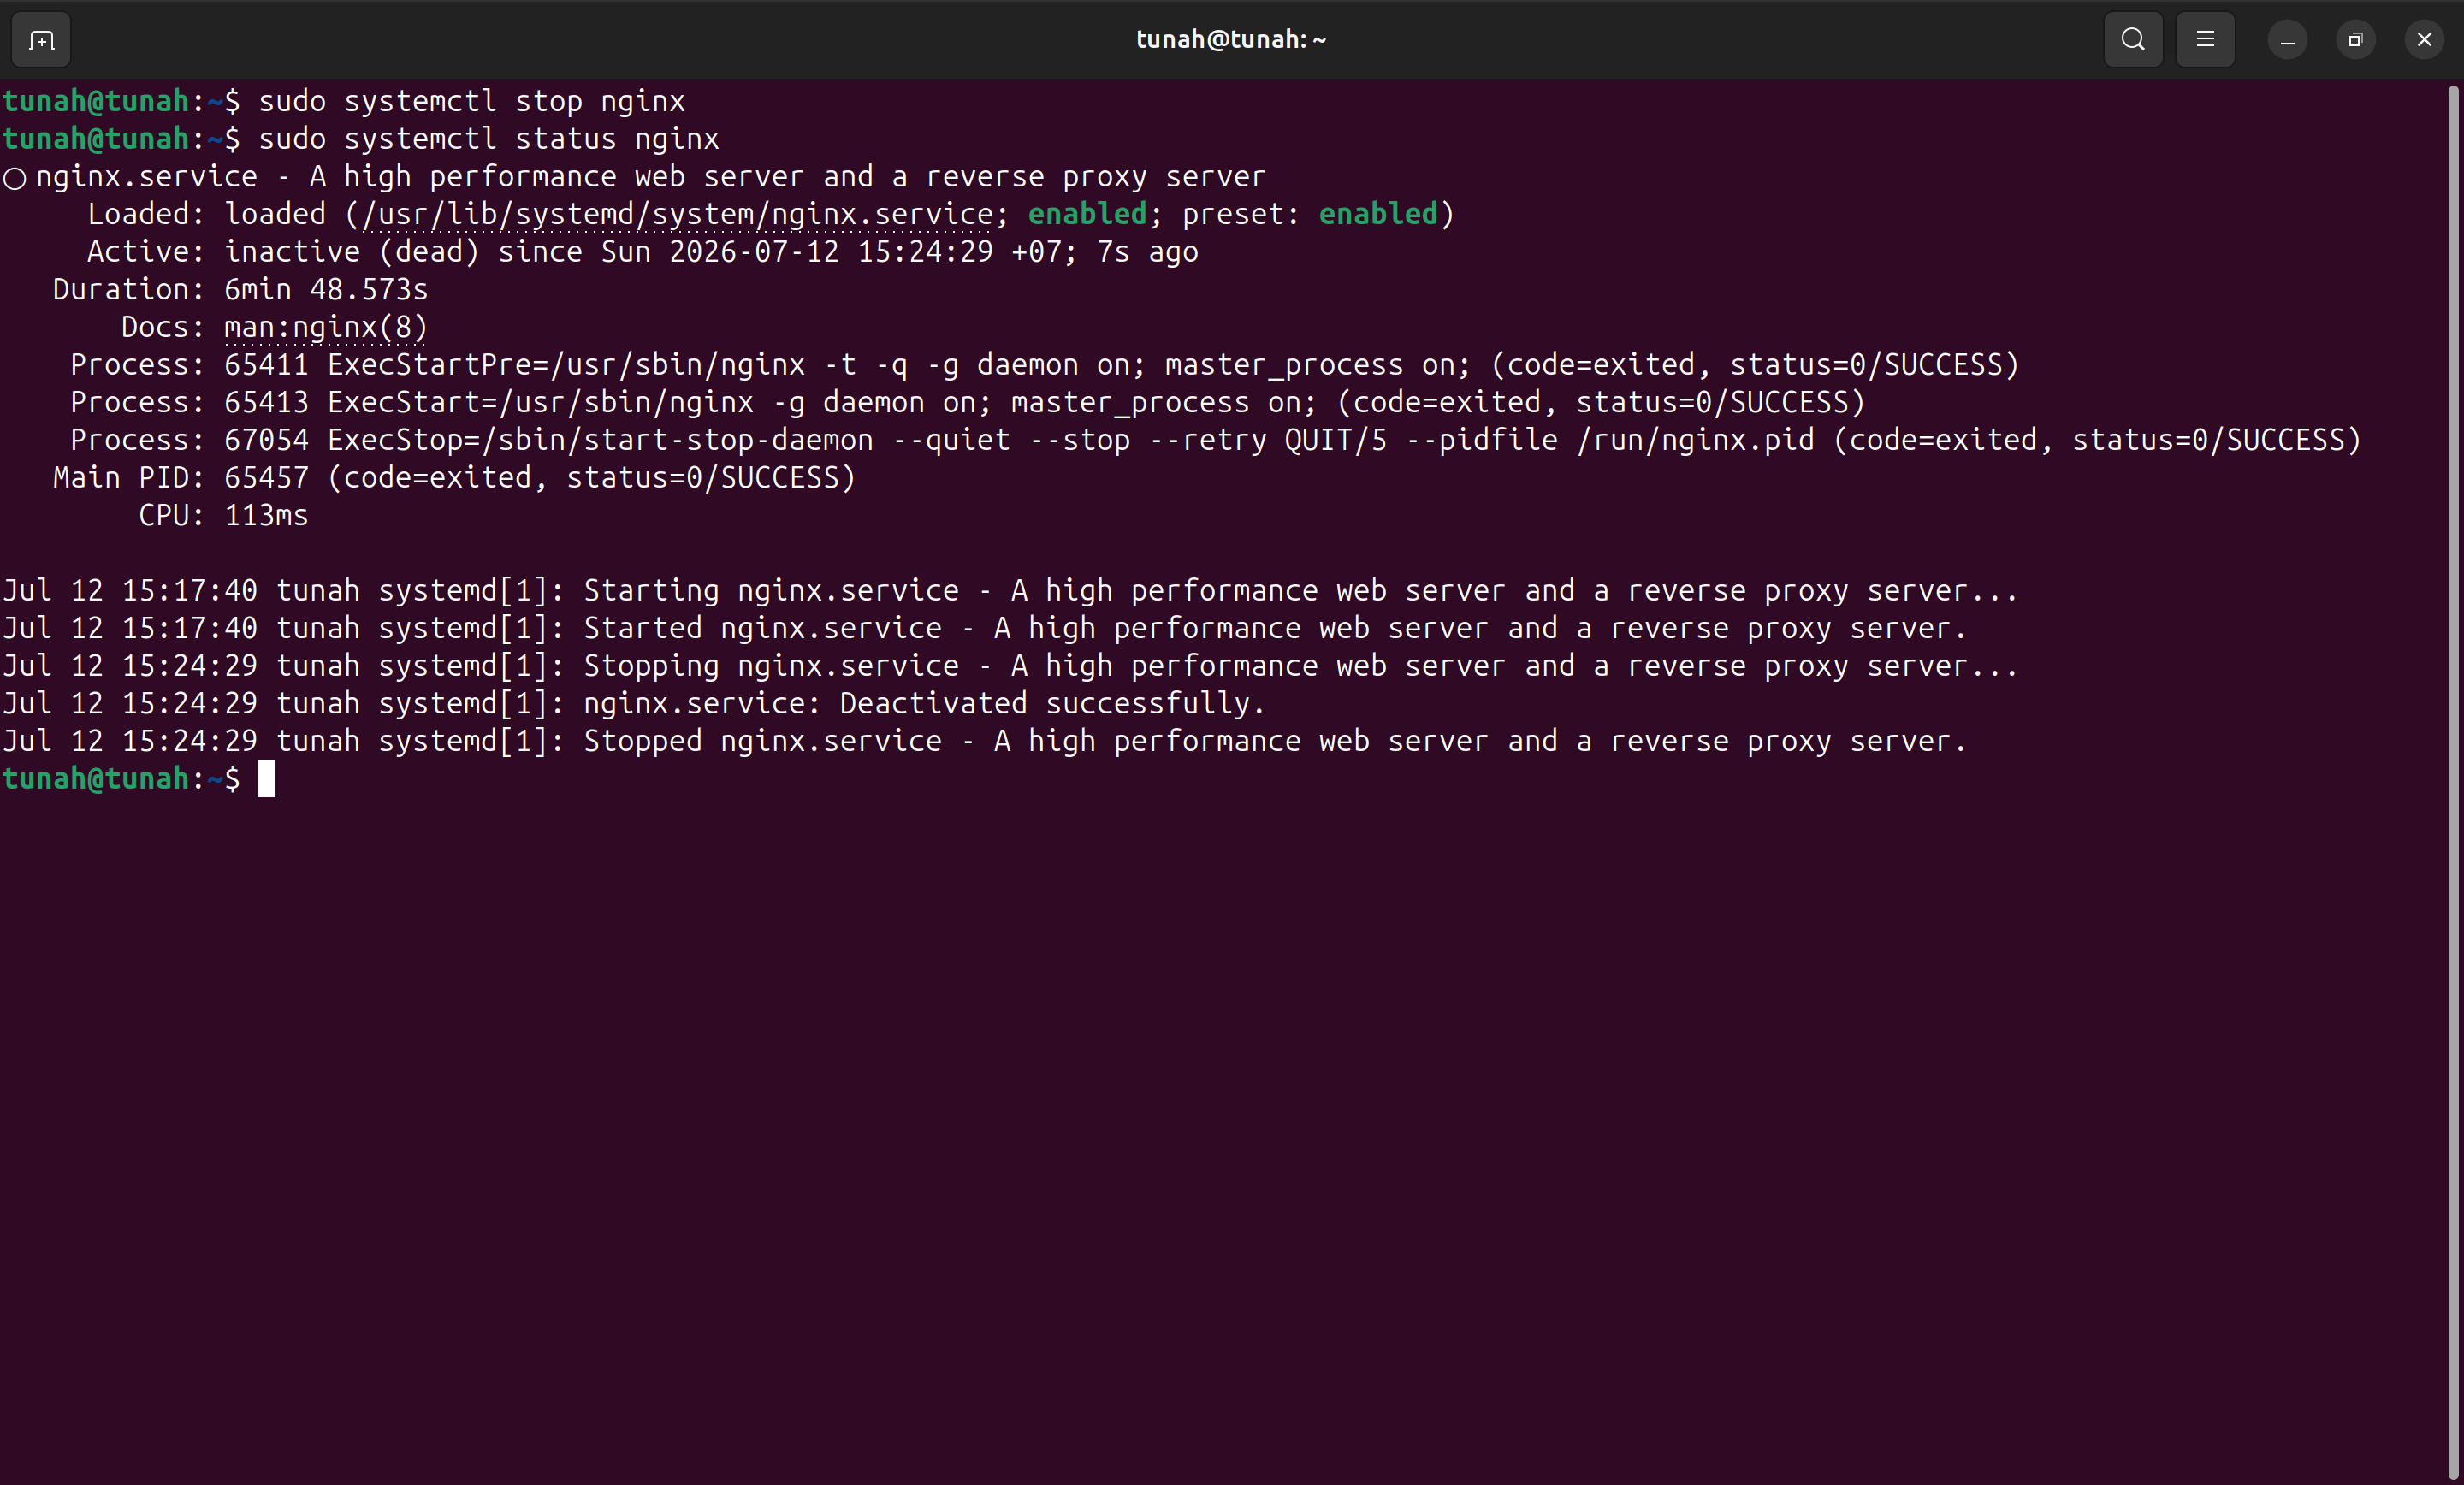
\includegraphics[width=\textwidth]{05/nginx-stopped.png}
        \caption{Nginx inactive}
    \end{subfigure}
    \caption{Quản lý trạng thái service}
\end{figure}

\subsection{Cấu hình Khởi động cùng hệ thống}

\textbf{Cách thực hiện:}
Tắt và bật tính năng tự động khởi động cùng hệ thống của Nginx. Kiểm tra lại bằng cờ \texttt{is-enabled}.

\begin{lstlisting}[language=bash]
sudo systemctl disable nginx
systemctl is-enabled nginx

sudo systemctl enable nginx
systemctl is-enabled nginx
\end{lstlisting}

\textbf{Kết quả:}
Trạng thái hiển thị \texttt{disabled} rồi chuyển thành \texttt{enabled}, xác nhận Nginx sẽ tự boot khi khởi động máy.

\begin{figure}[H]
    \centering
    \begin{subfigure}[b]{0.48\textwidth}
        \centering
        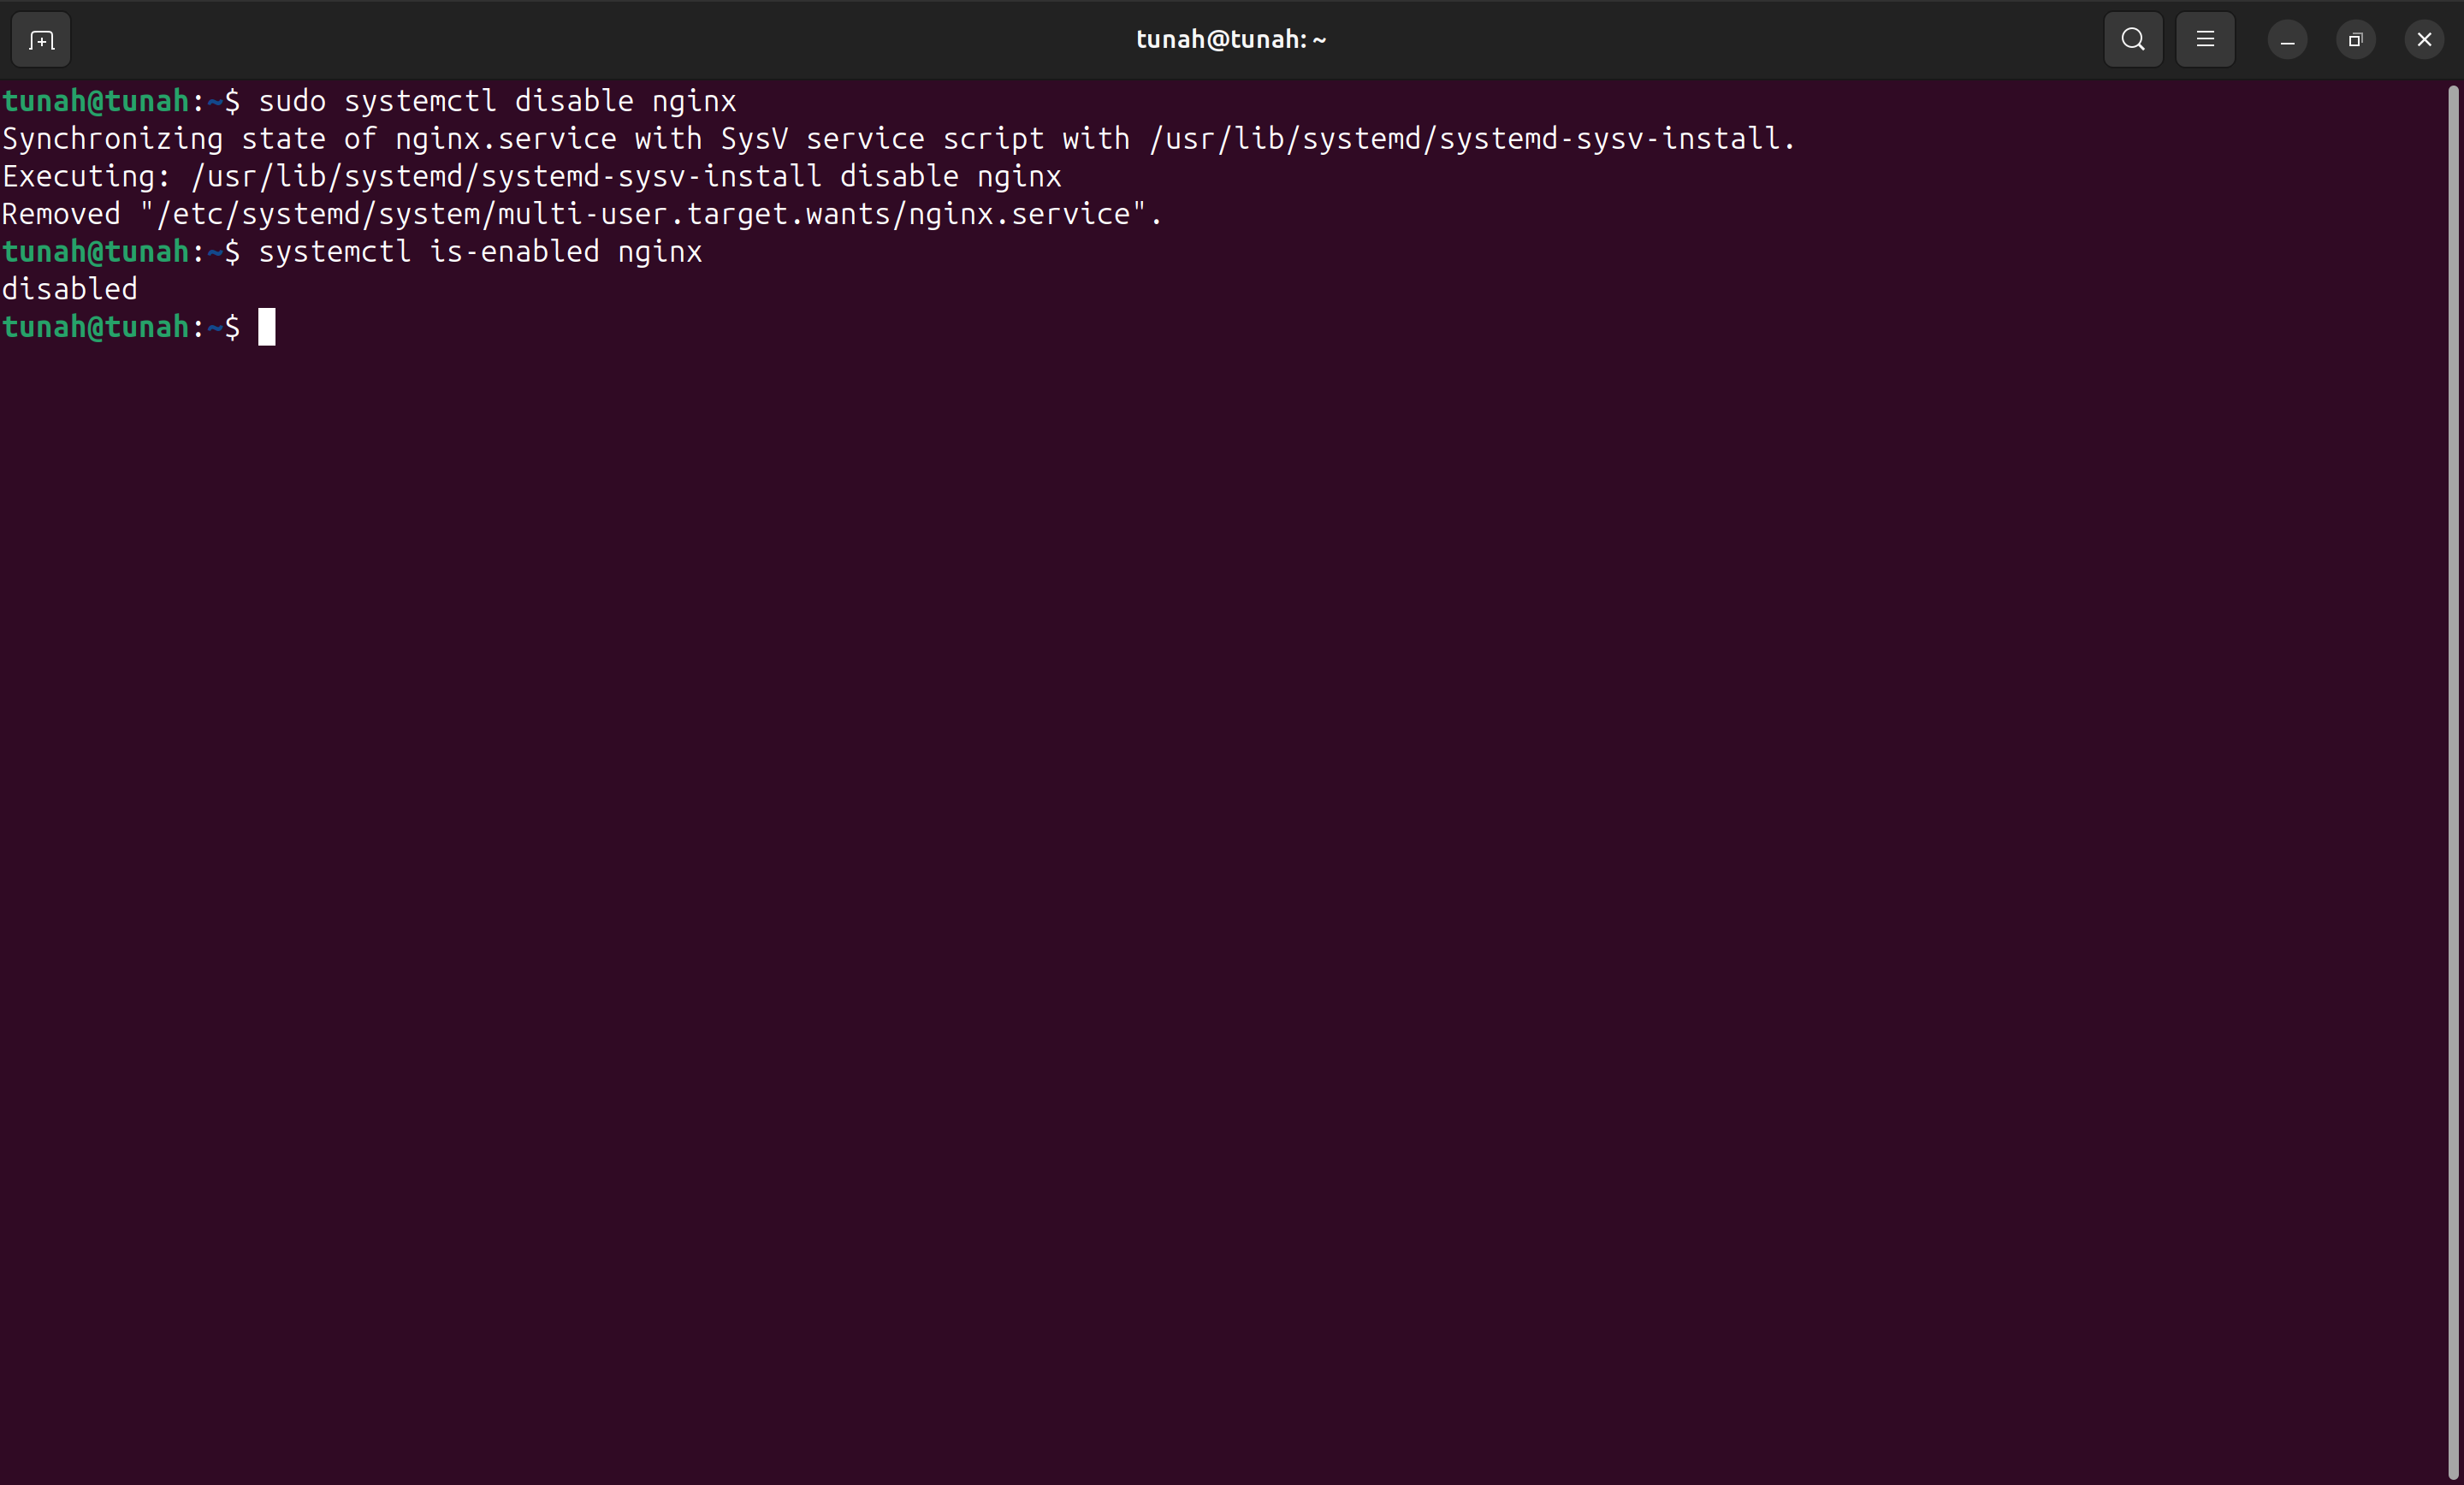
\includegraphics[width=\textwidth]{05/nginx-disabled.png}
        \caption{Disable Nginx}
    \end{subfigure}
    \hfill
    \begin{subfigure}[b]{0.48\textwidth}
        \centering
        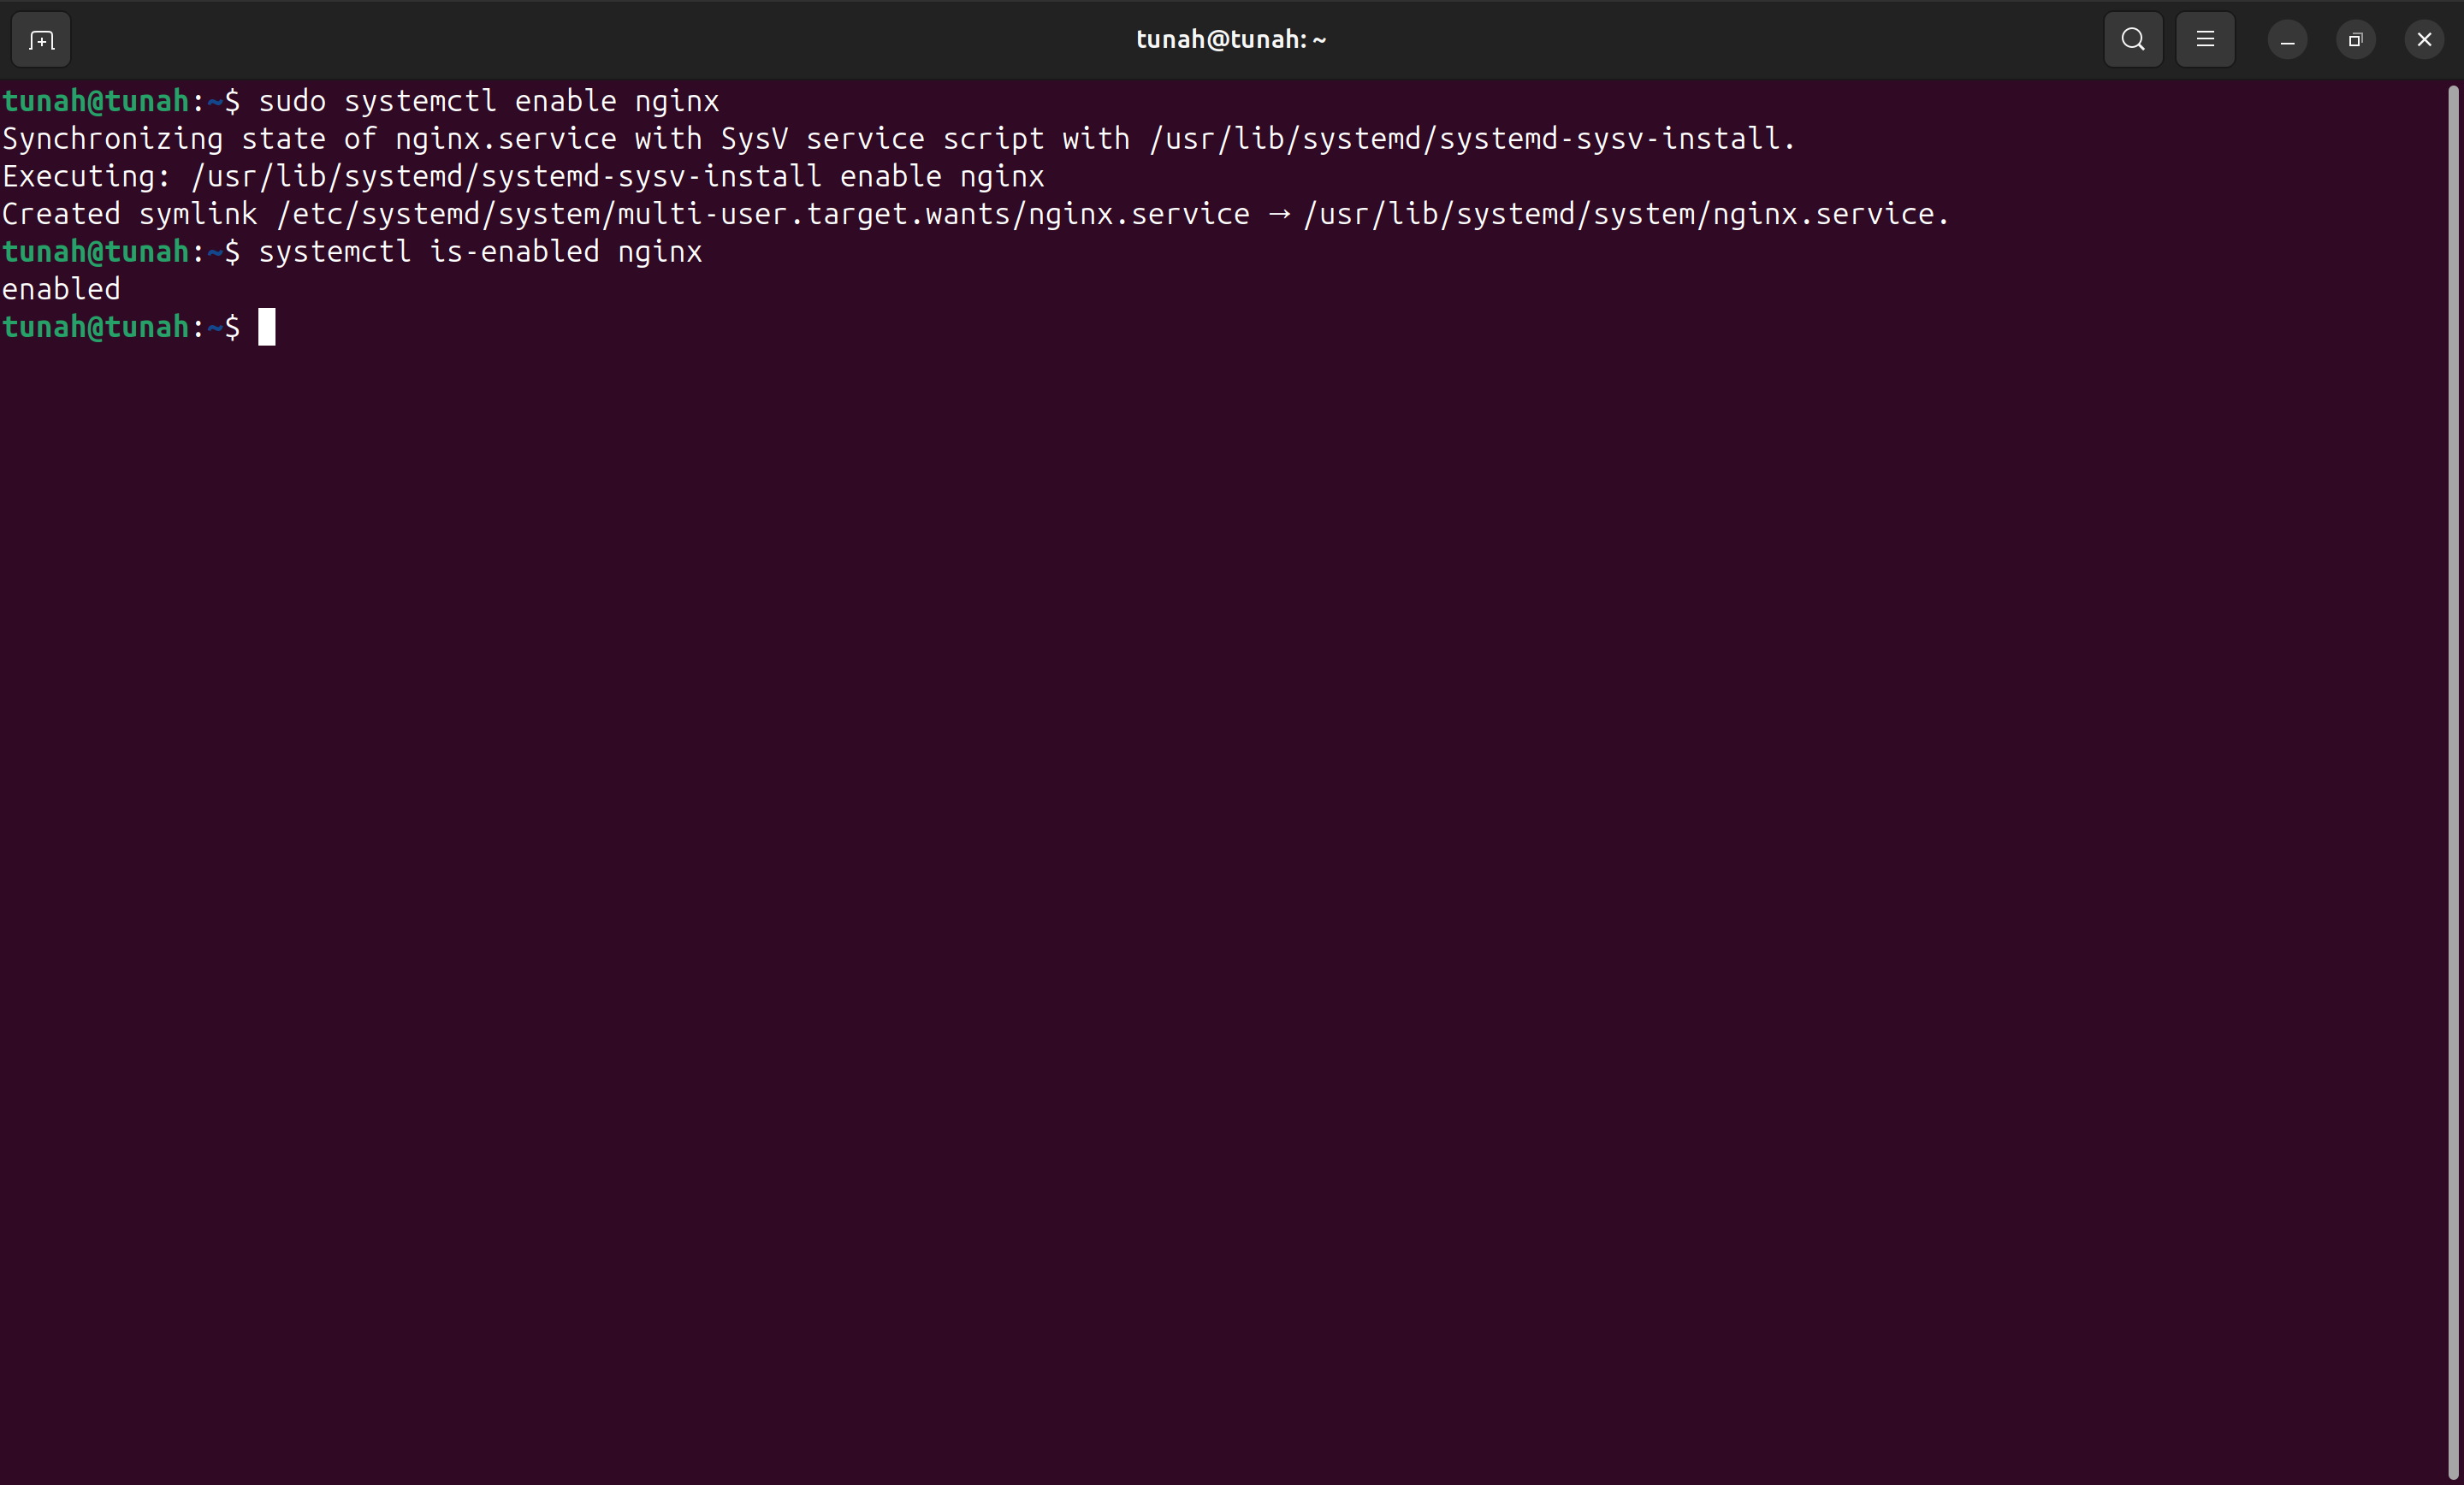
\includegraphics[width=\textwidth]{05/nginx-enabled.png}
        \caption{Enable Nginx}
    \end{subfigure}
    \caption{Cấu hình Autostart}
\end{figure}

\subsection{Kiểm tra và Theo dõi File Log}

\textbf{Cách thực hiện:}
- Dùng \texttt{curl} truy cập \texttt{localhost} để tạo request thành công. Đọc file \texttt{access.log}.
- Đọc file \texttt{error.log} để xem lỗi.
- Chạy \texttt{tail -f} để xem log lỗi theo thời gian thực (realtime) khi gửi request sai.

\begin{lstlisting}[language=bash]
# Tao request va xem access log
curl http://localhost
sudo cat /var/log/nginx/access.log

# Xem error log va tail realtime
sudo cat /var/log/nginx/error.log
sudo tail -f /var/log/nginx/error.log
\end{lstlisting}

\textbf{Kết quả:}
Hệ thống ghi nhận chính xác các truy cập (mã 200) và các lỗi truy cập trang không tồn tại (mã 404). Lệnh \texttt{tail -f} giúp giám sát server hiệu quả.

\begin{figure}[H]
    \centering
    \begin{subfigure}[b]{0.45\textwidth}
        \centering
        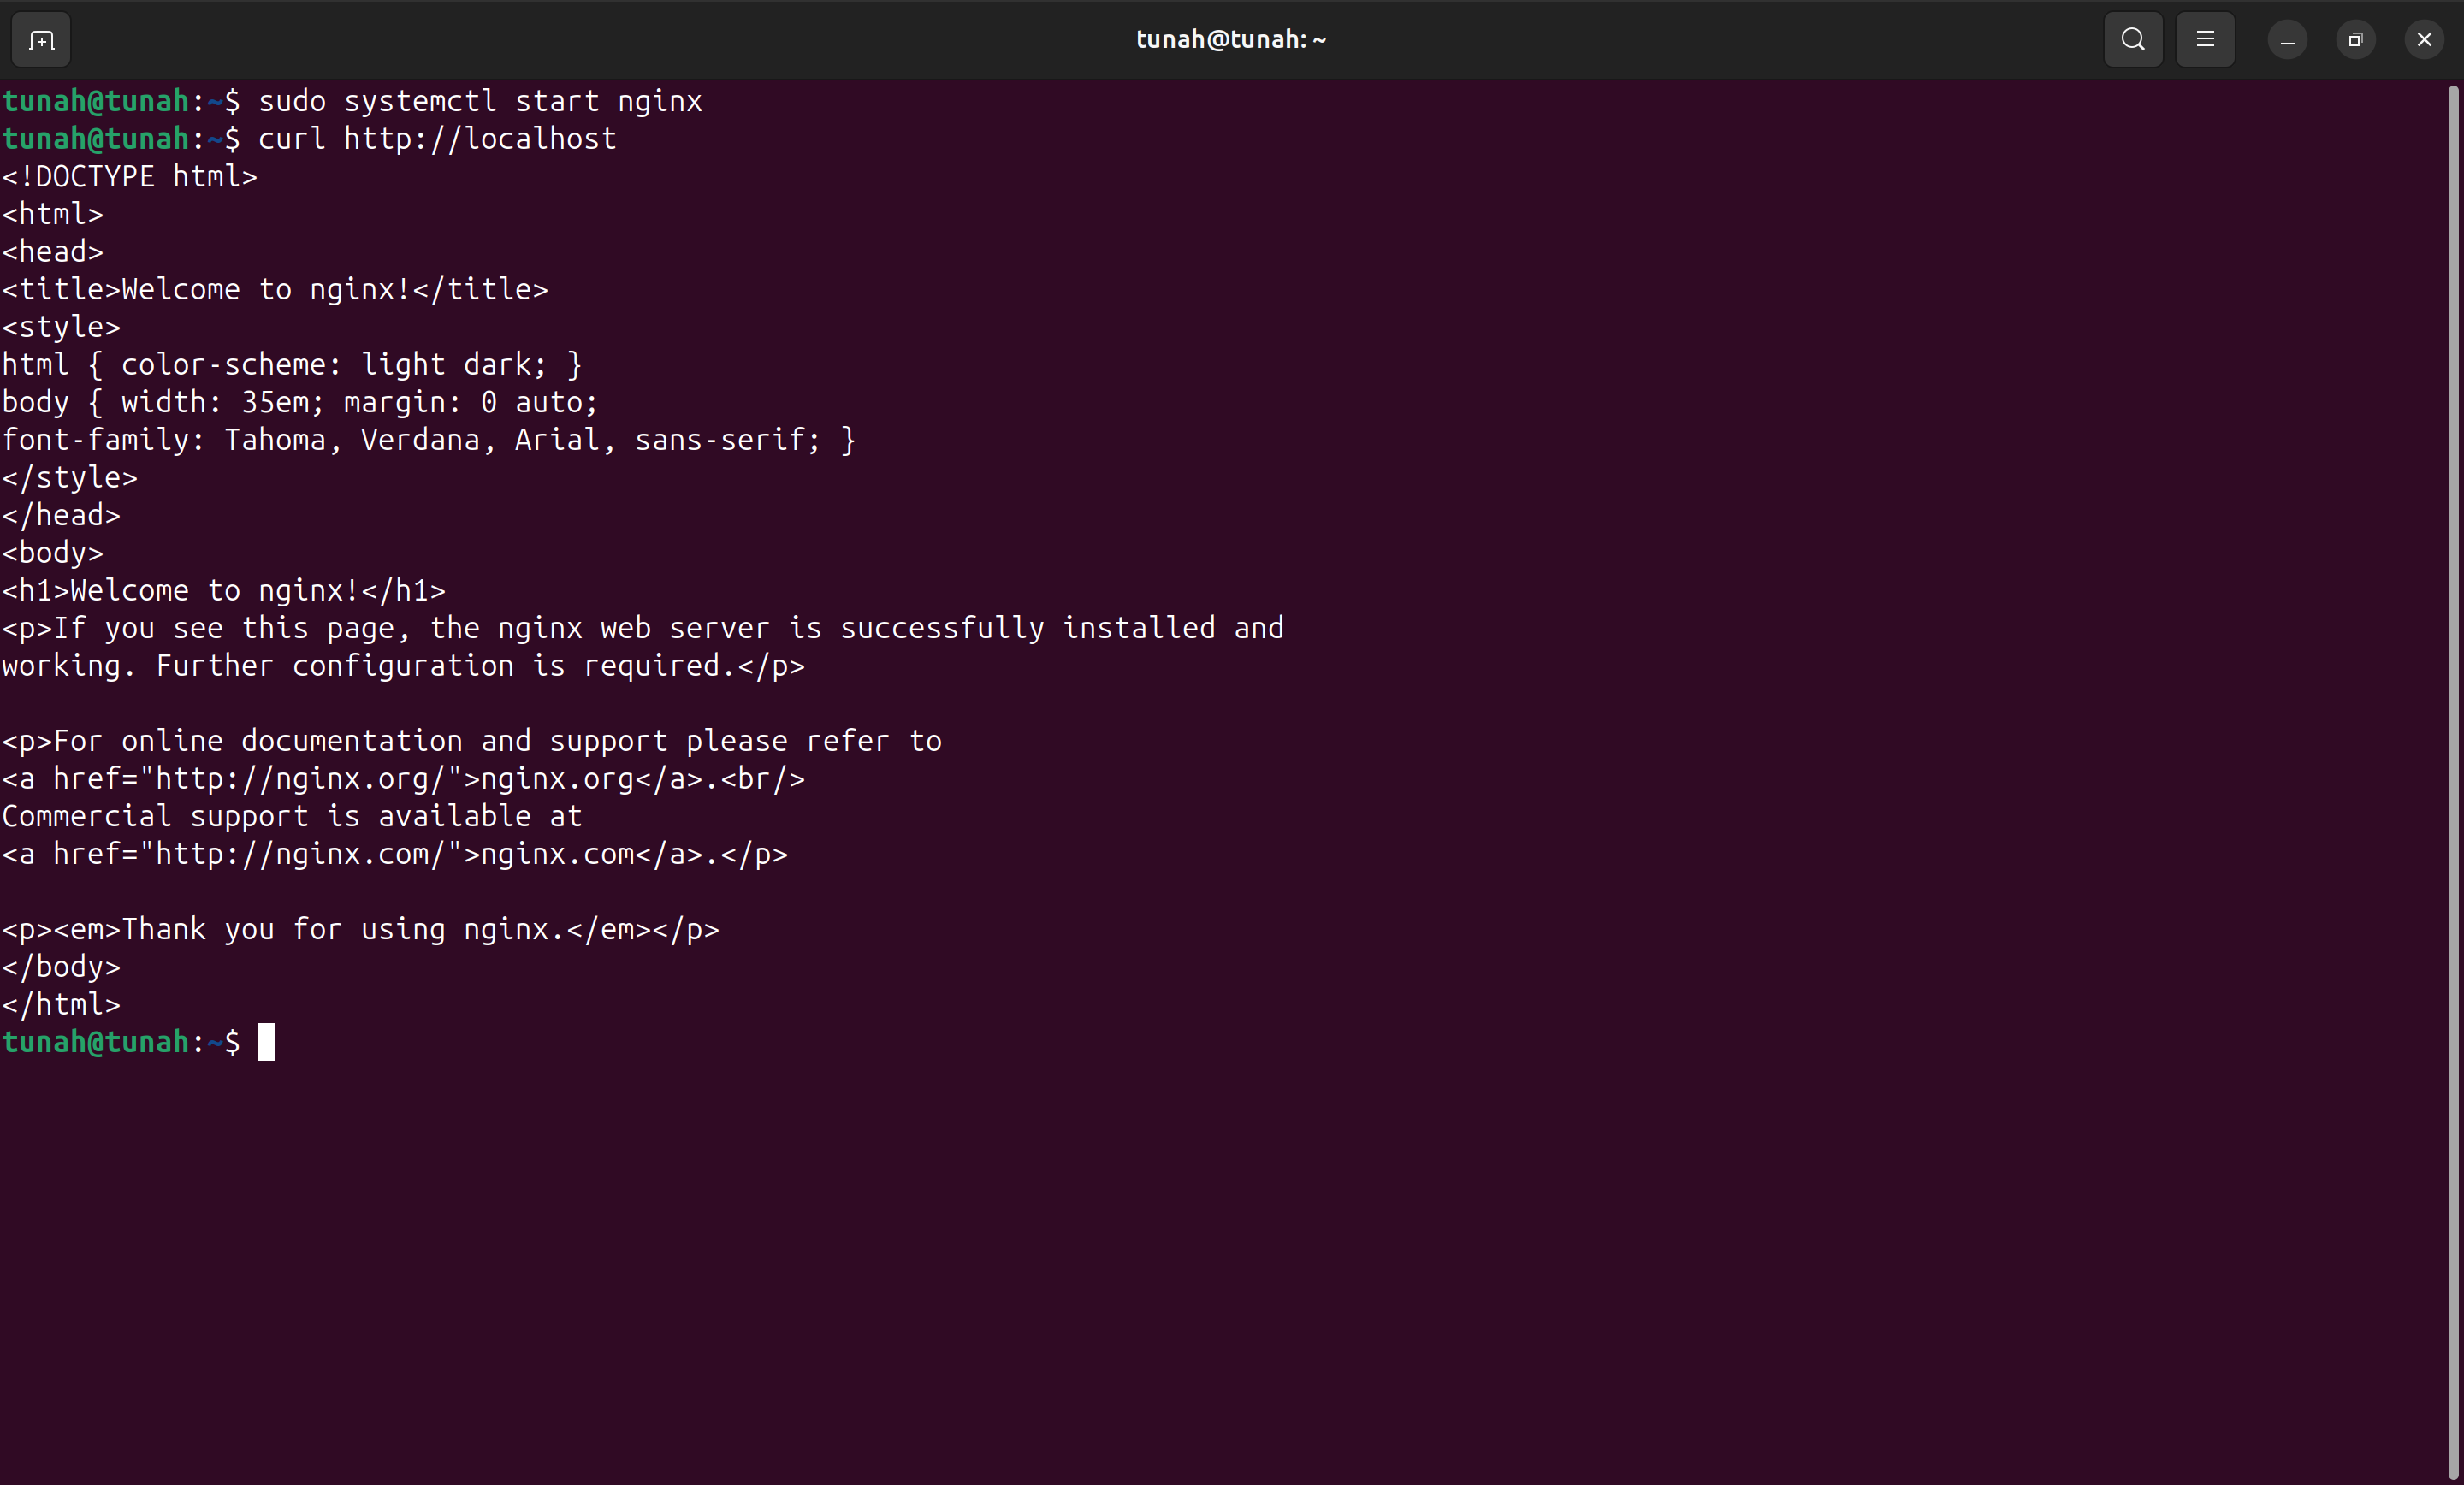
\includegraphics[width=\textwidth]{05/curl-localhost.png}
        \caption{Curl trang chủ}
    \end{subfigure}
    \hfill
    \begin{subfigure}[b]{0.45\textwidth}
        \centering
        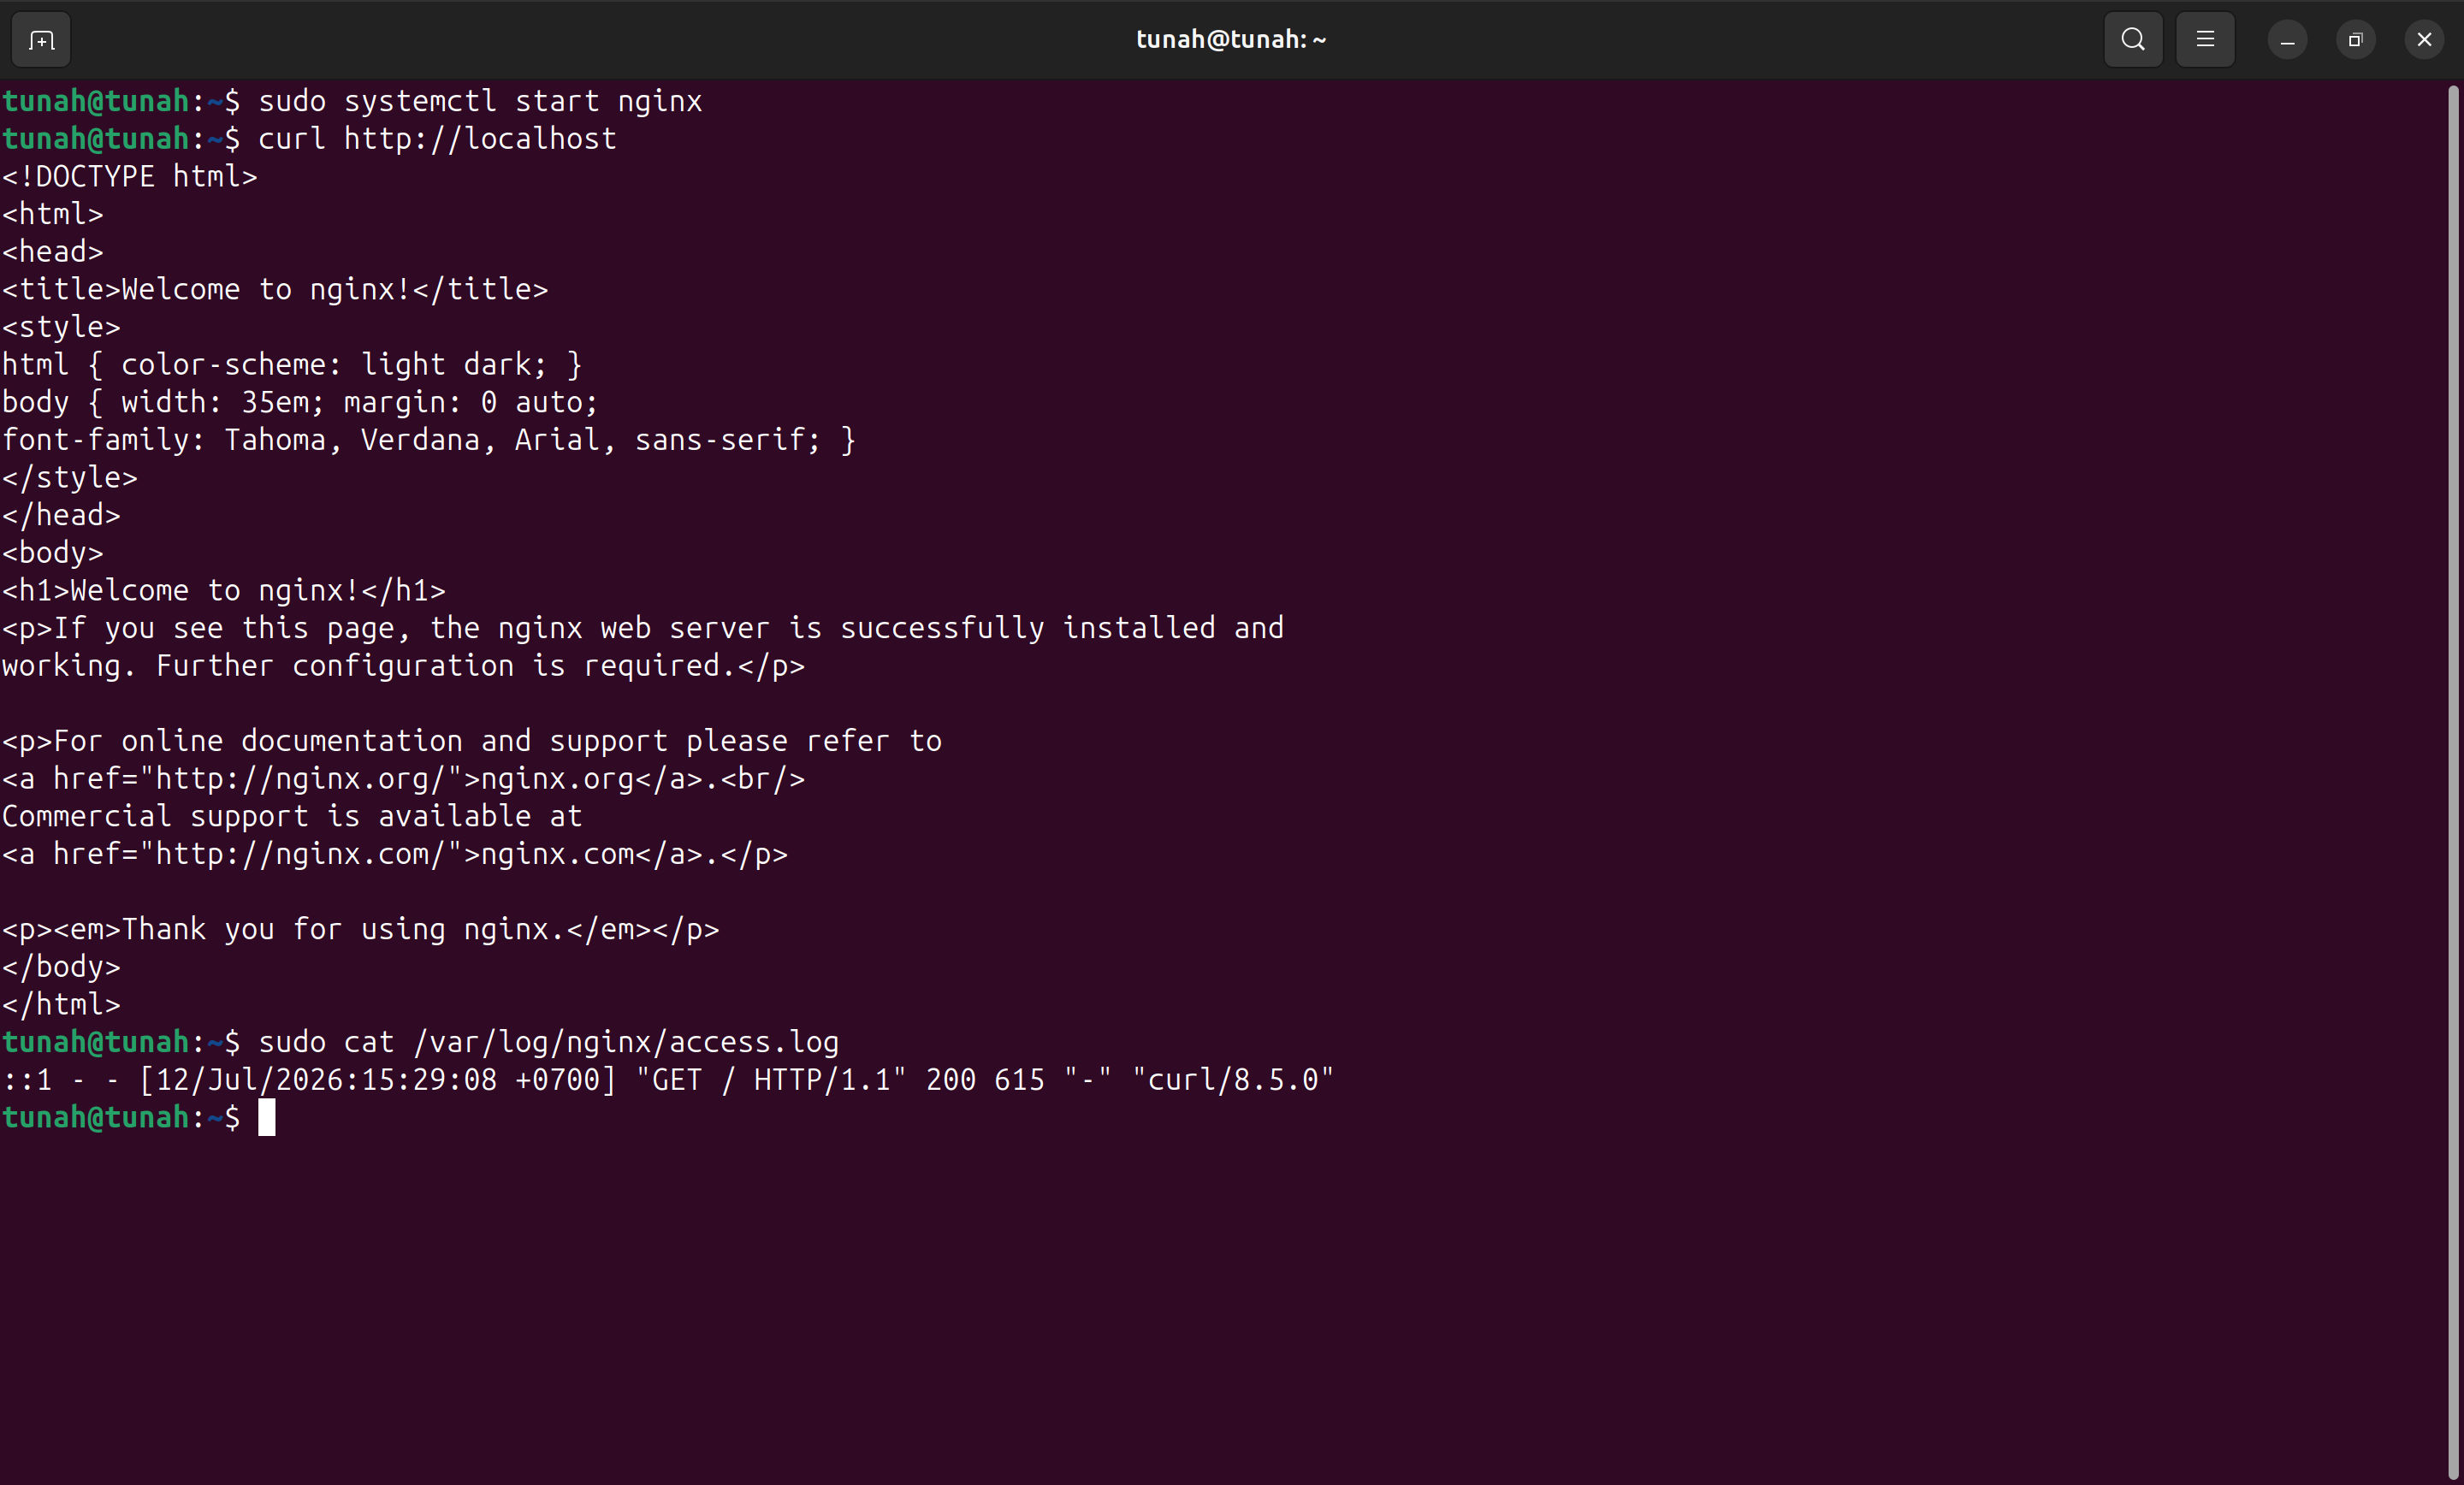
\includegraphics[width=\textwidth]{05/nginx-access-log.png}
        \caption{Access log ghi nhận truy cập}
    \end{subfigure}
    
    \vspace{0.5cm}
    \begin{subfigure}[b]{0.45\textwidth}
        \centering
        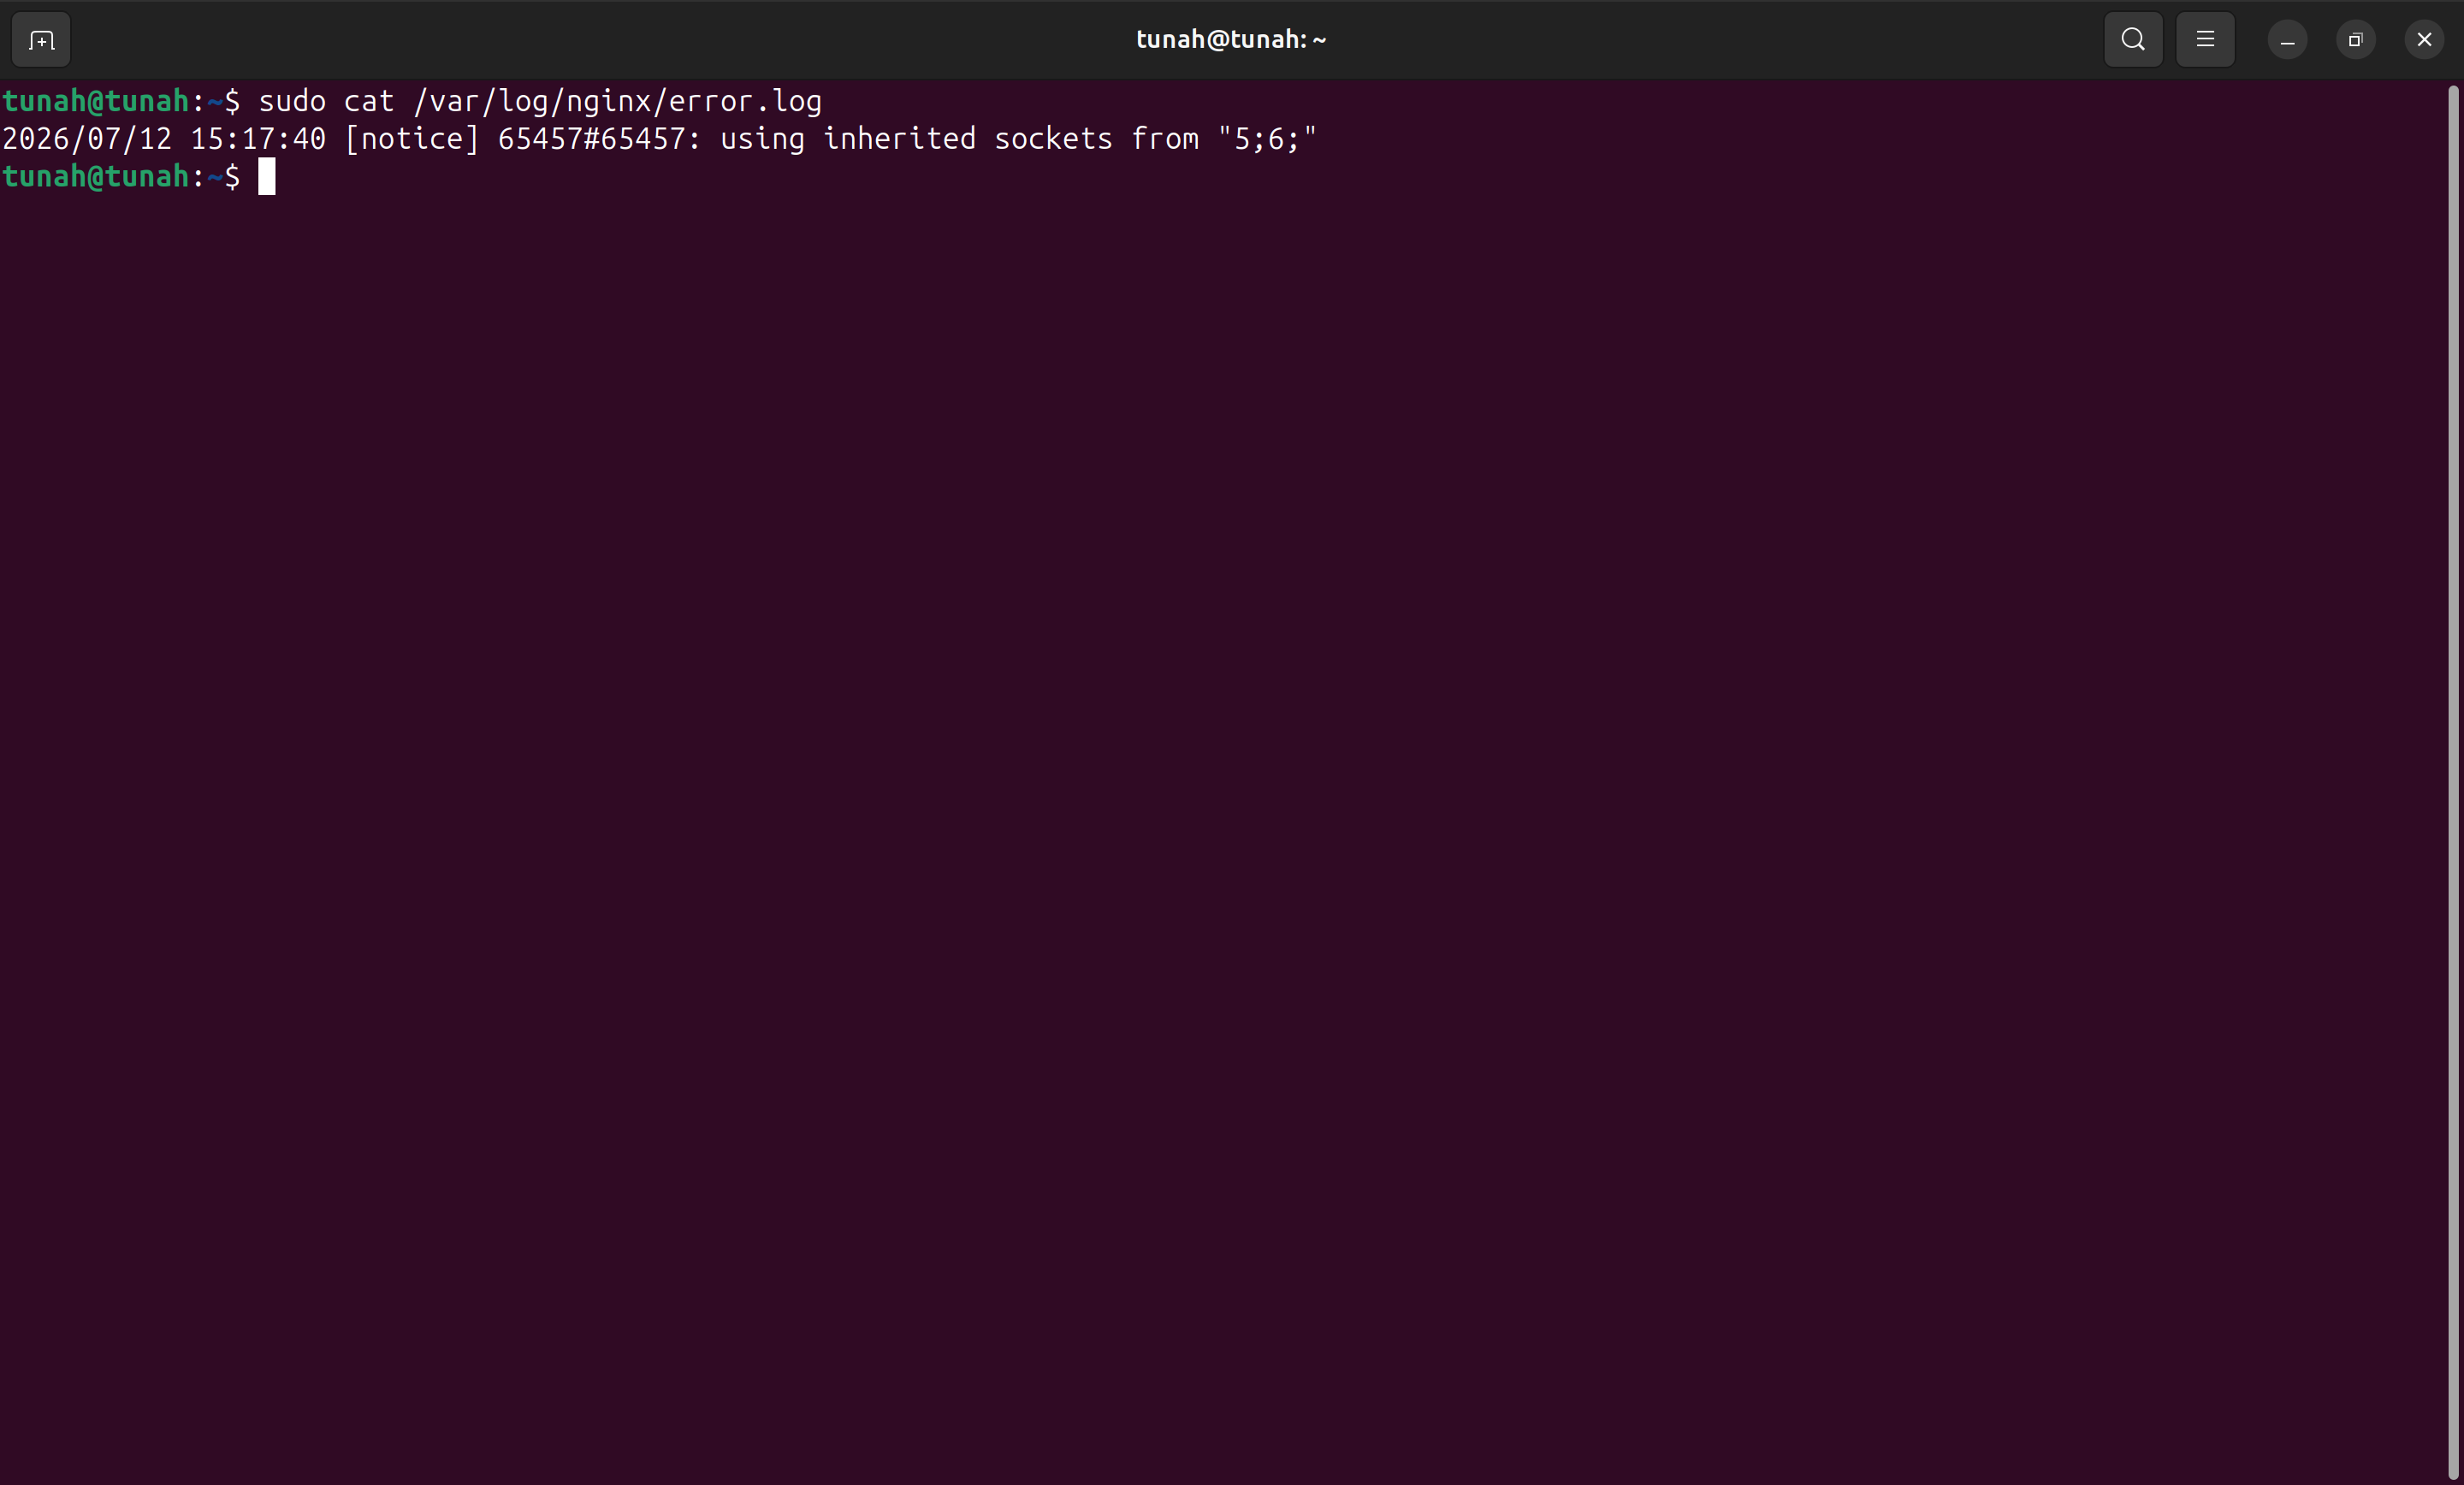
\includegraphics[width=\textwidth]{05/nginx-error-log.png}
        \caption{File Error log}
    \end{subfigure}
    \hfill
    \begin{subfigure}[b]{0.45\textwidth}
        \centering
        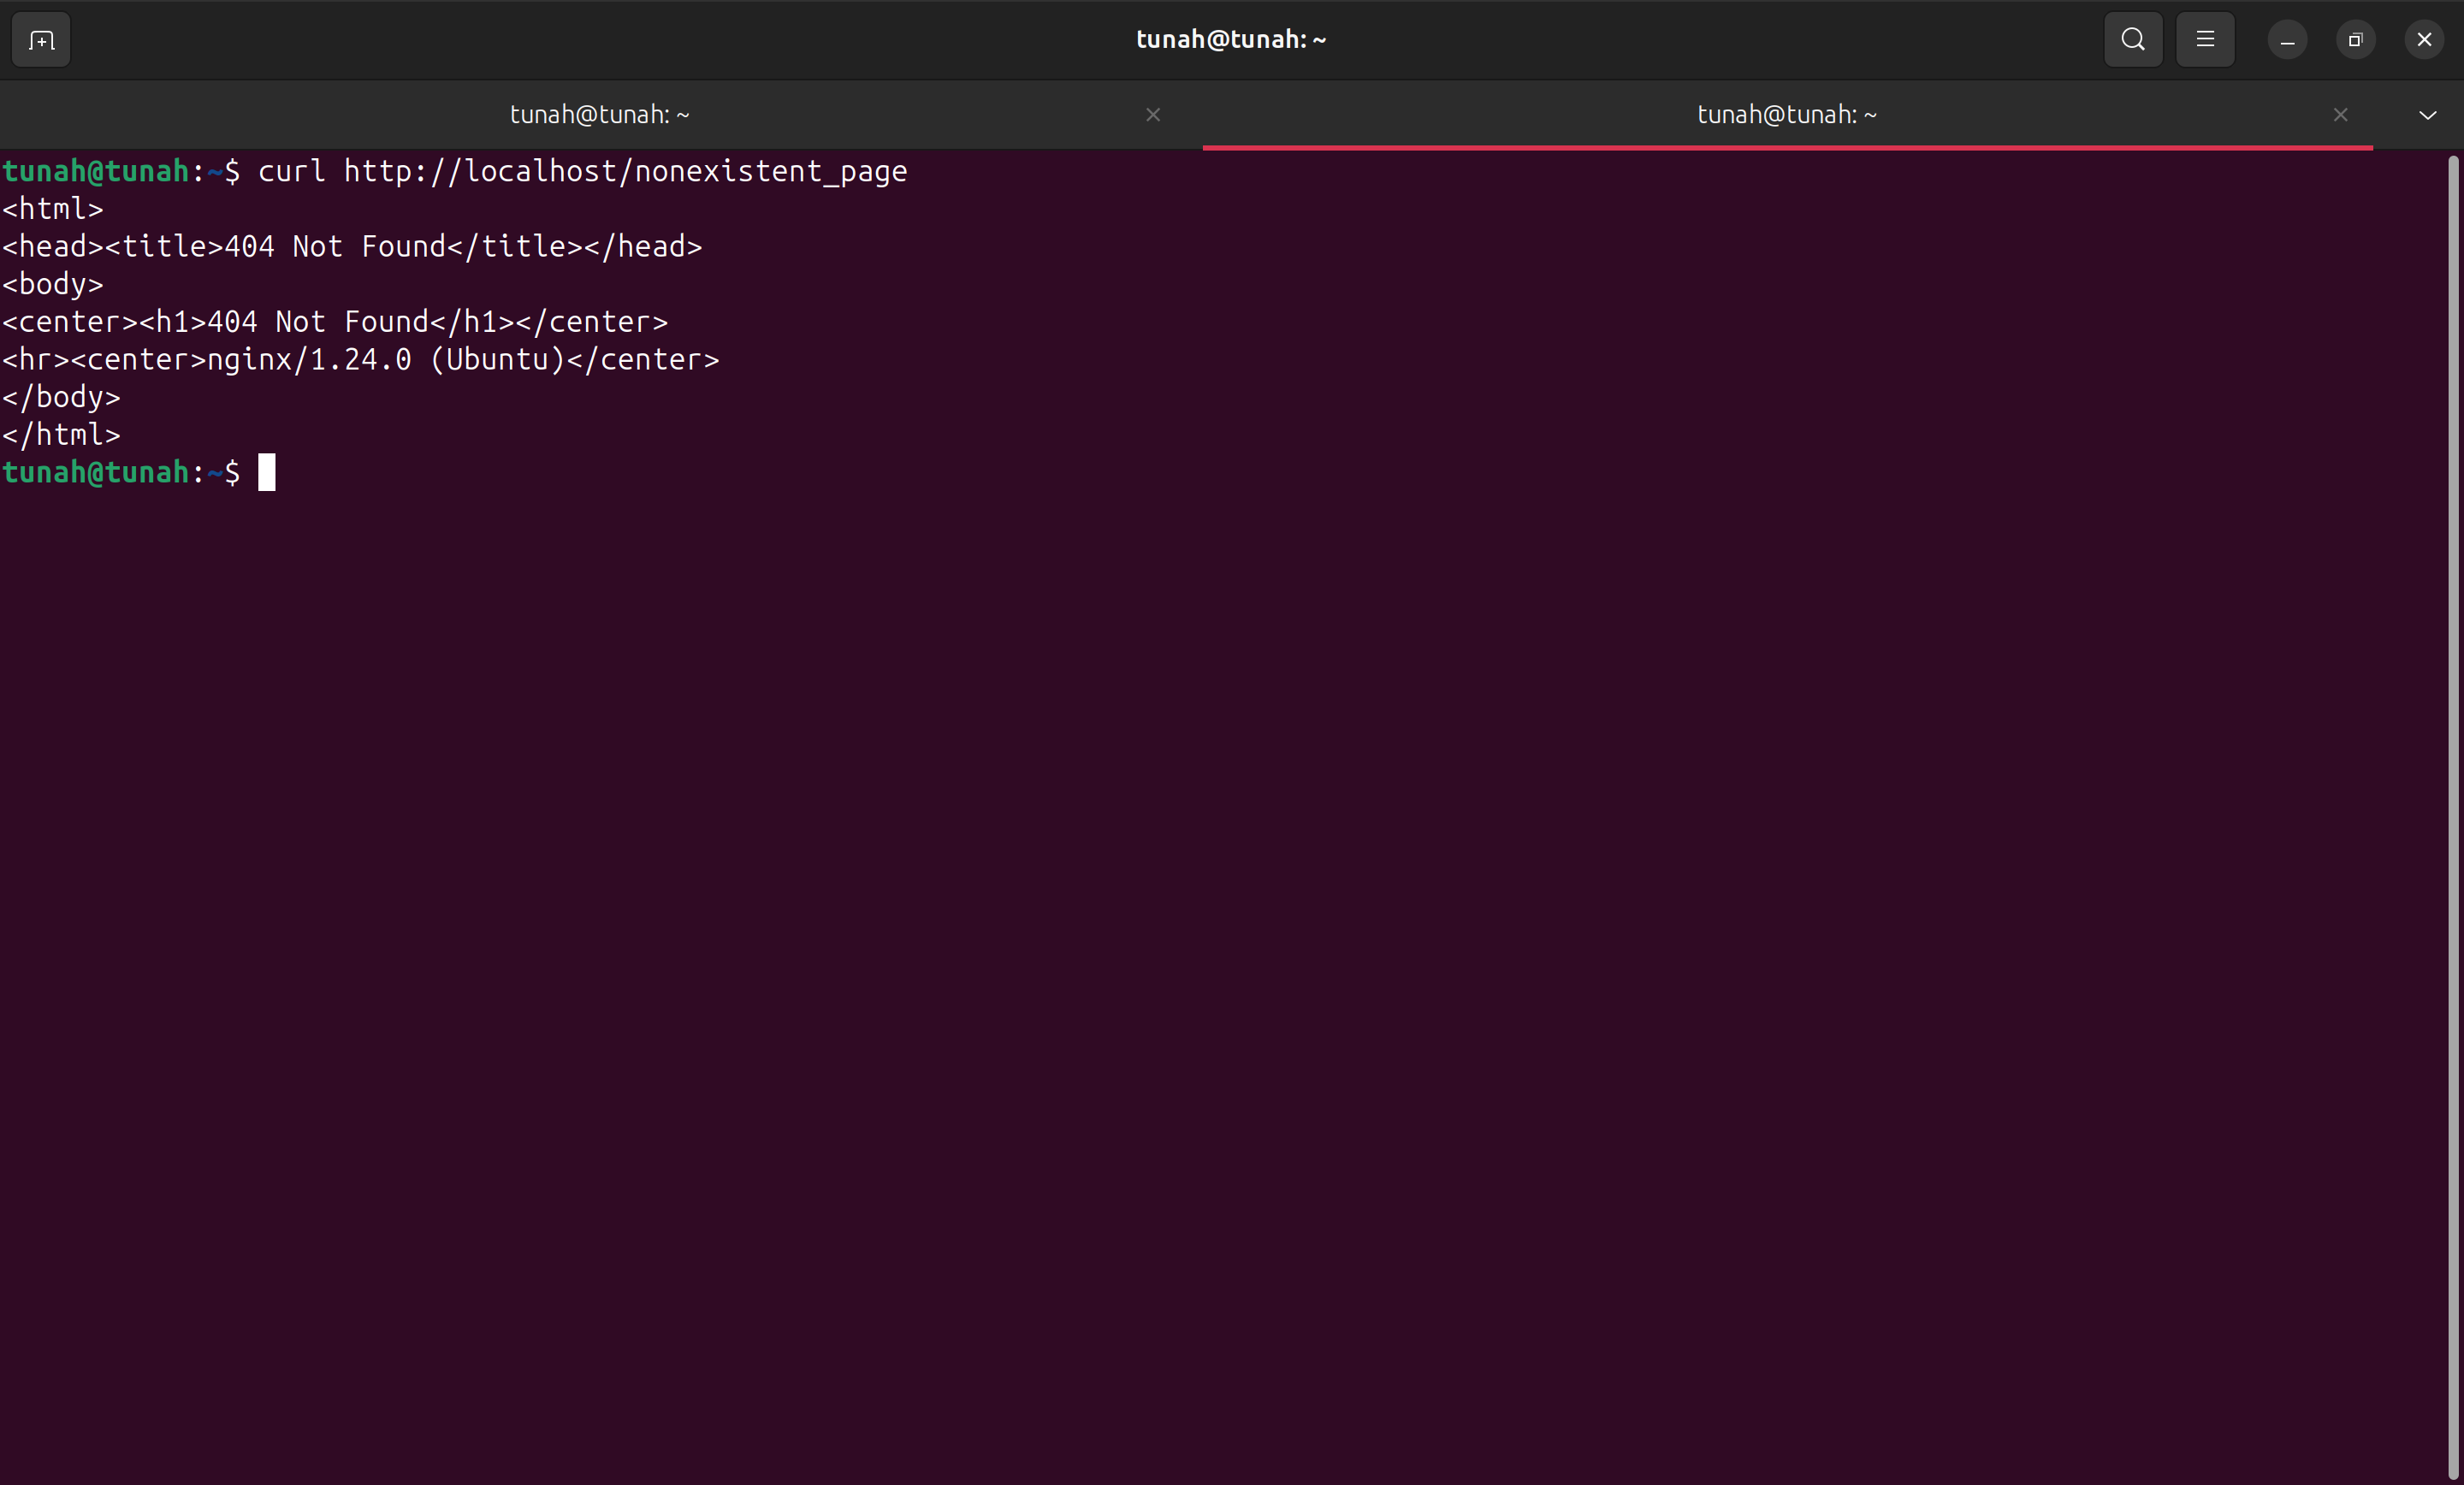
\includegraphics[width=\textwidth]{05/nginx-tail-realtime.png}
        \caption{Theo dõi Error log realtime}
    \end{subfigure}
    \caption{Quản lý và giám sát File Log}
\end{figure}

\section{Quản lý tác vụ tự động bằng Bash Script}

\subsection{Cơ bản về Script: In nội dung, Biến và Tính toán}

\textbf{Cách thực hiện:}
Tạo các script cơ bản để làm quen với Bash:
- \texttt{hello.sh}: In ra chuỗi "Hello World".
- \texttt{current\_time.sh}: Lấy kết quả từ lệnh \texttt{date} và in ra ngày giờ hệ thống.
- \texttt{sum.sh}: Sử dụng lệnh \texttt{read} để nhận đầu vào từ bàn phím và tính tổng 2 số.

\begin{lstlisting}[language=bash]
# Cap quyen va chay cac script da tao
chmod +x hello.sh current_time.sh sum.sh
./hello.sh
./current_time.sh
./sum.sh
\end{lstlisting}

\textbf{Kết quả:}
Các script chạy ổn định, tiếp nhận được Input từ người dùng và xử lý các câu lệnh command line lồng ghép chính xác.

\begin{figure}[H]
    \centering
    \begin{subfigure}[b]{0.32\textwidth}
        \centering
        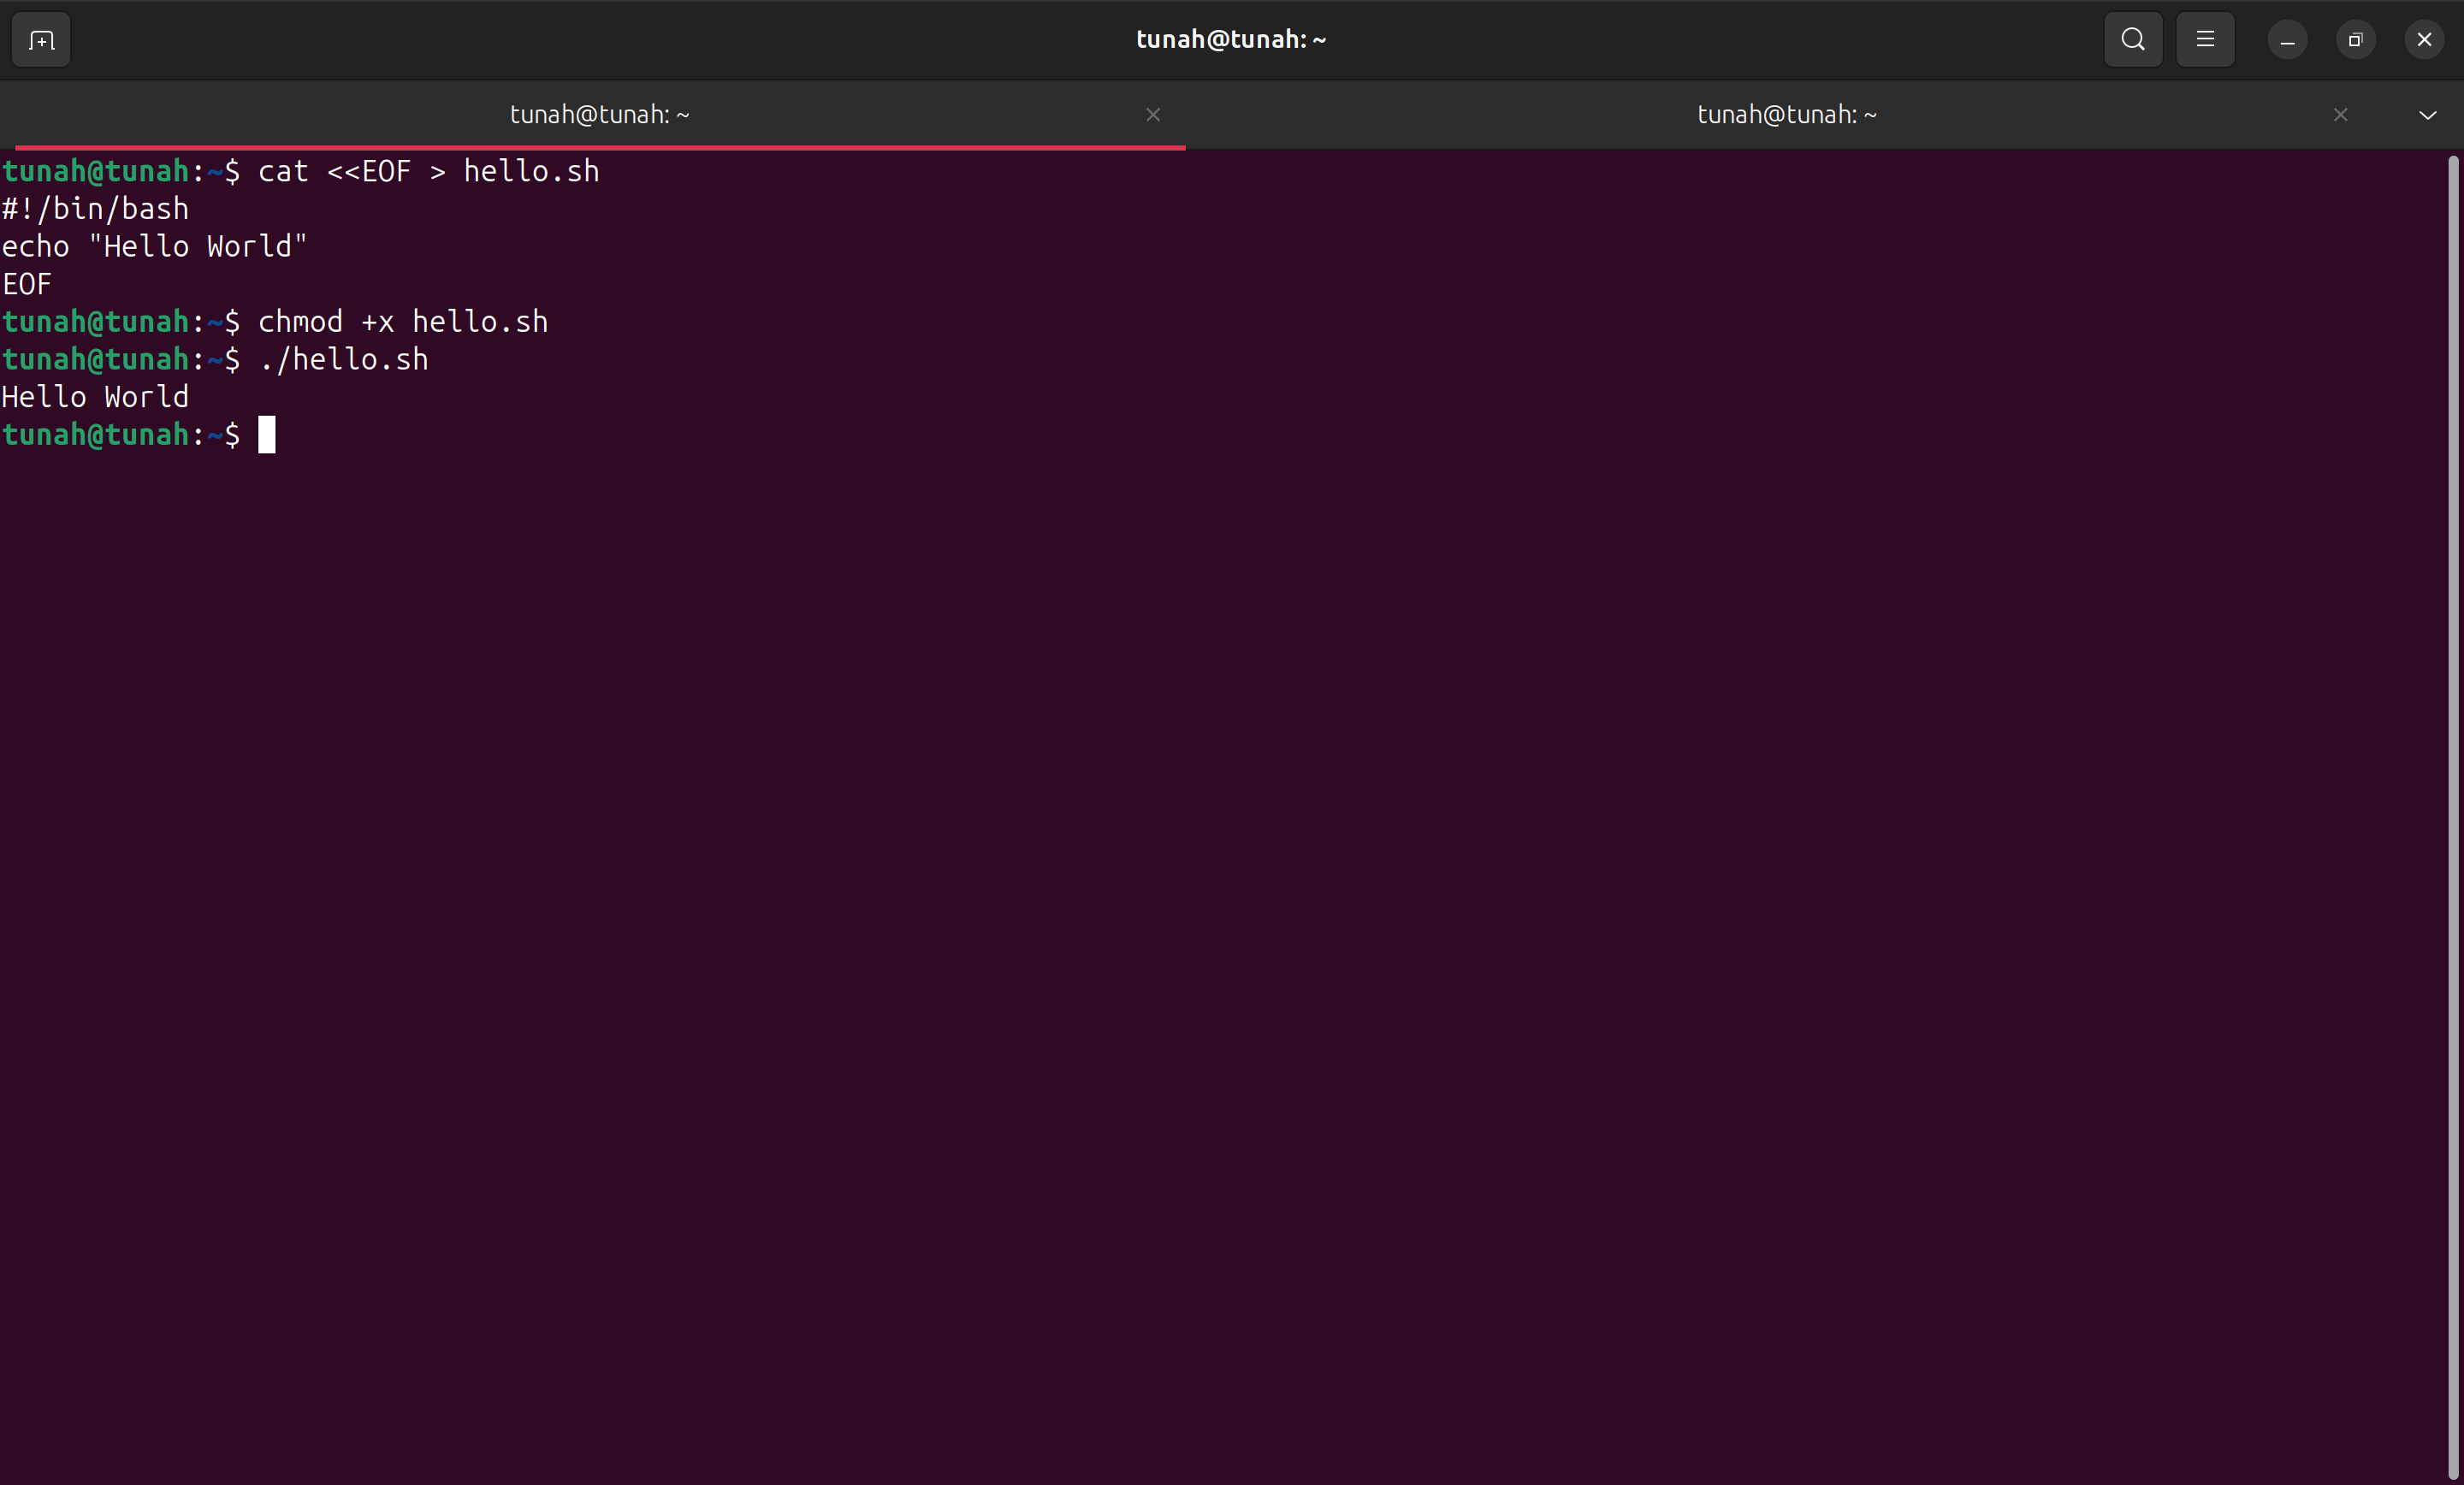
\includegraphics[width=\textwidth]{07/hello-world-script.png}
        \caption{In Hello World}
    \end{subfigure}
    \hfill
    \begin{subfigure}[b]{0.32\textwidth}
        \centering
        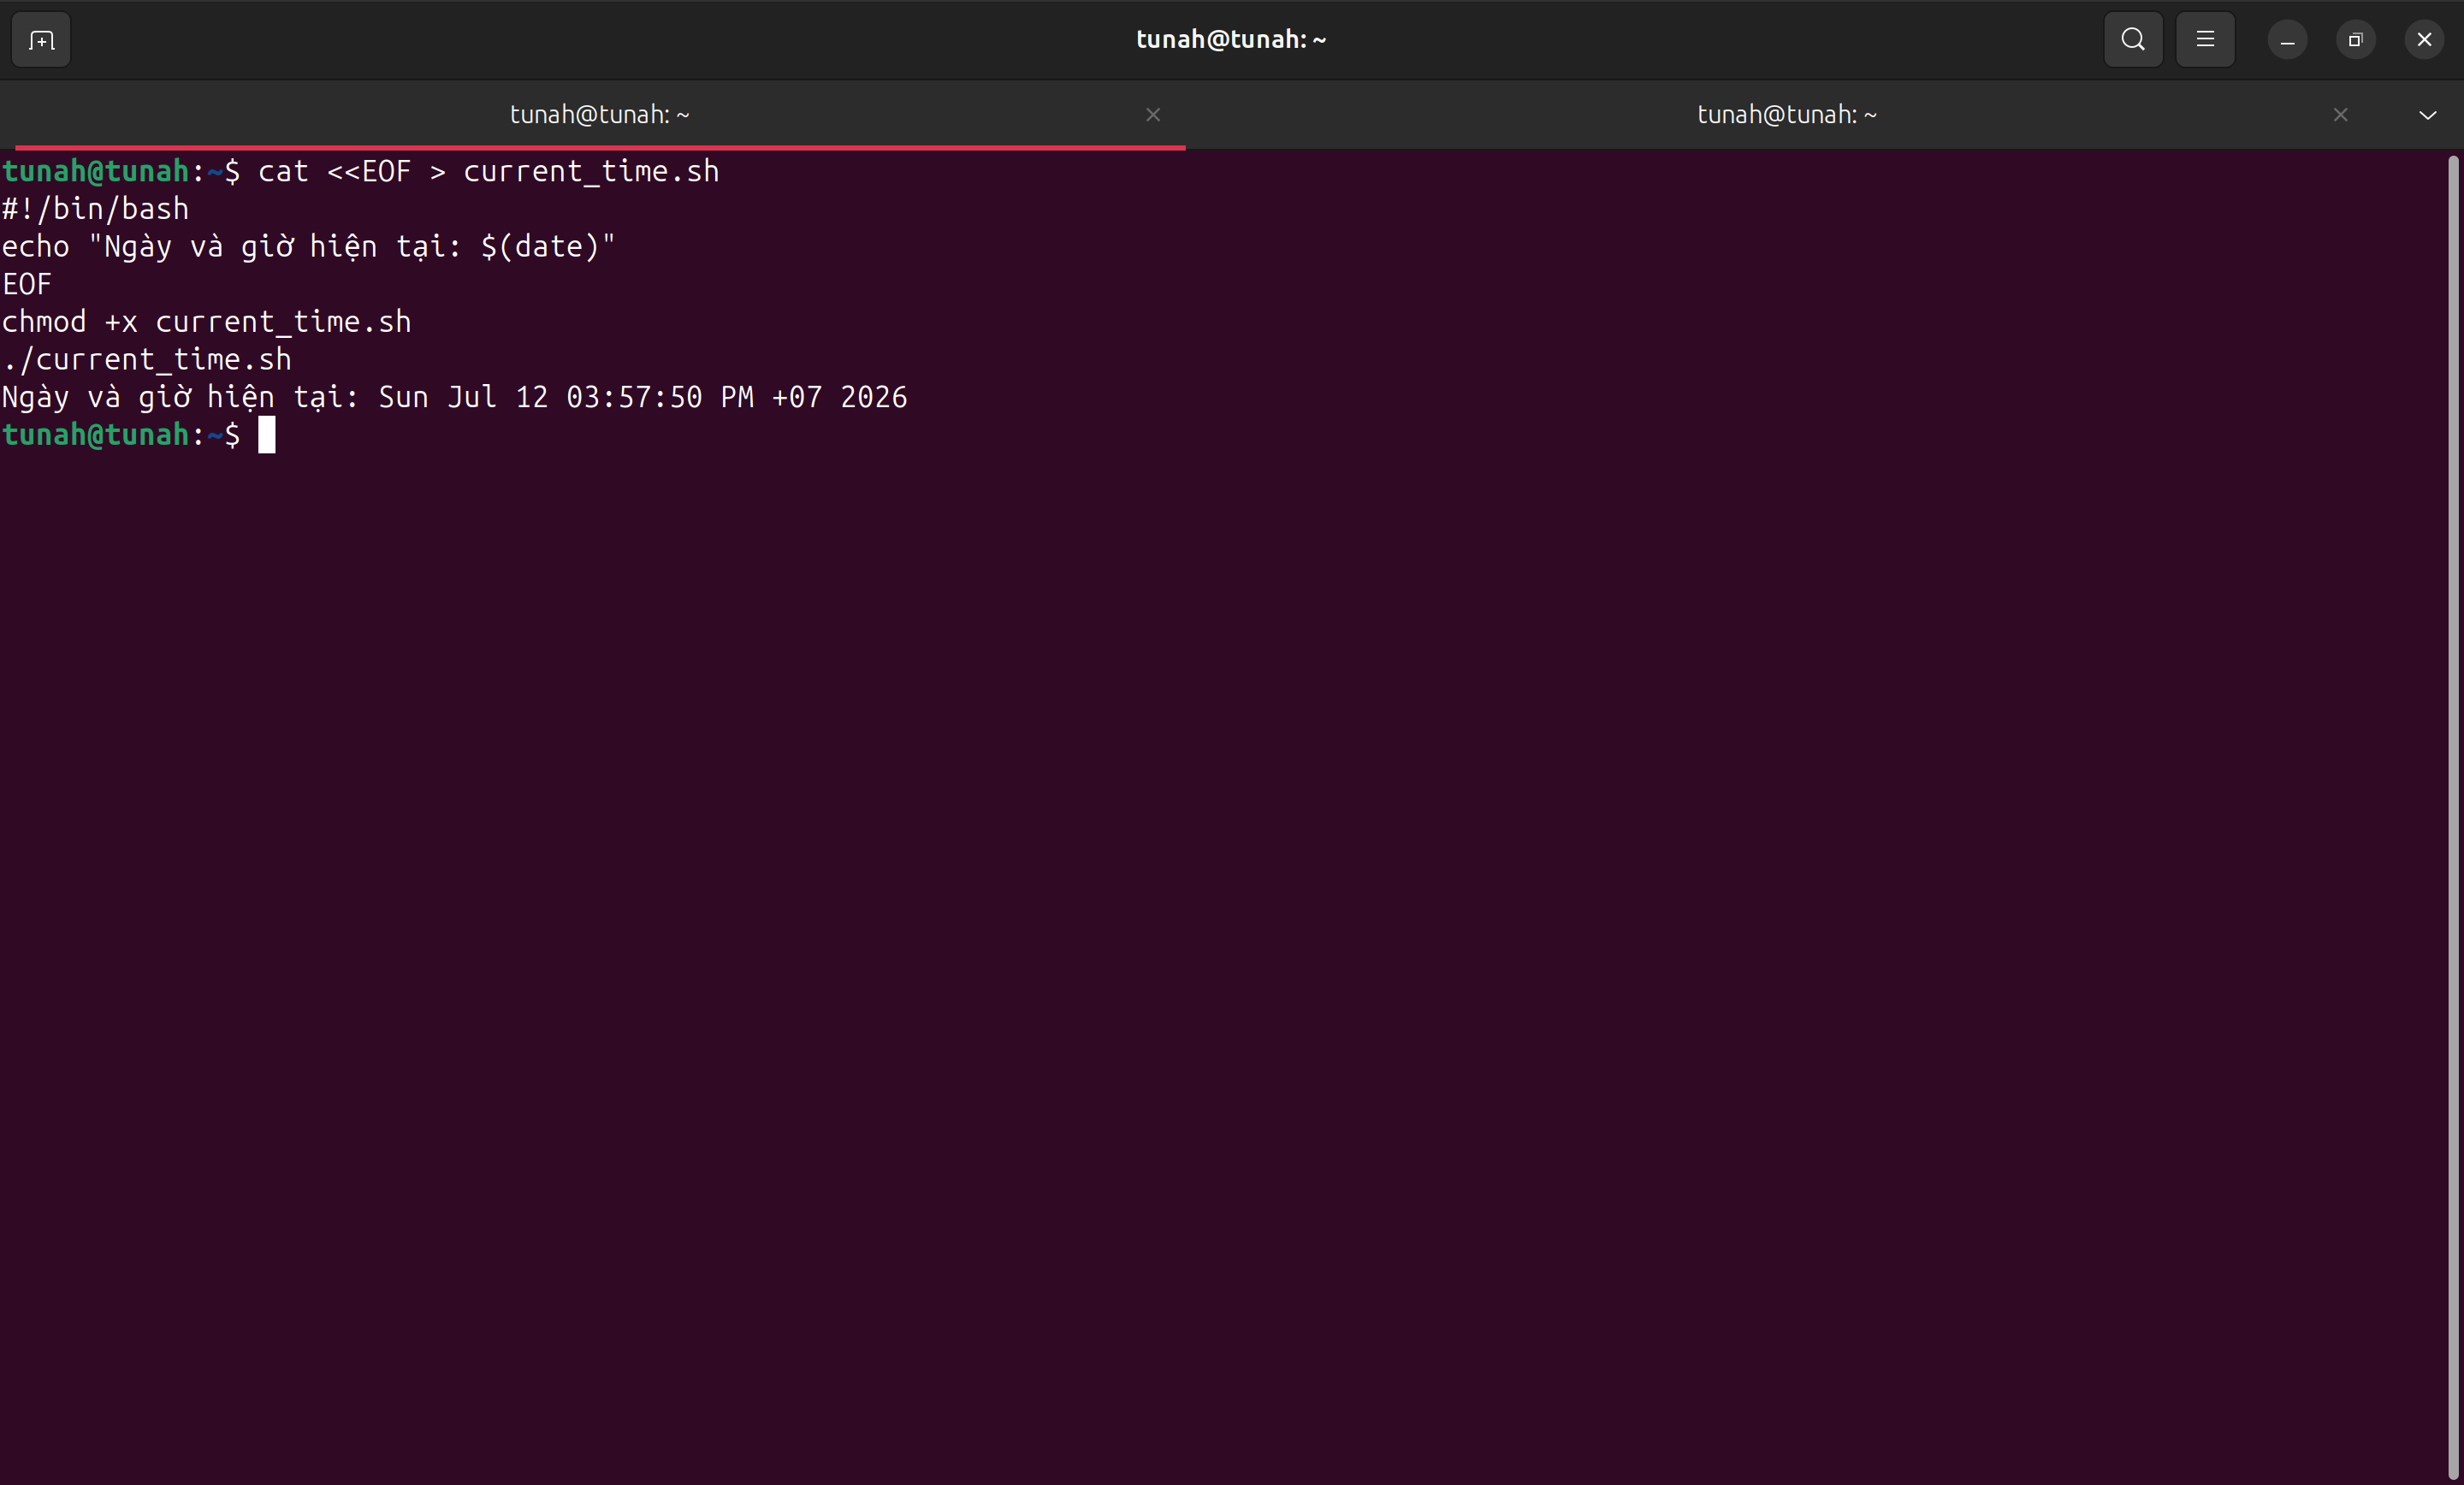
\includegraphics[width=\textwidth]{07/current-time-script.png}
        \caption{In ngày giờ hệ thống}
    \end{subfigure}
    \hfill
    \begin{subfigure}[b]{0.32\textwidth}
        \centering
        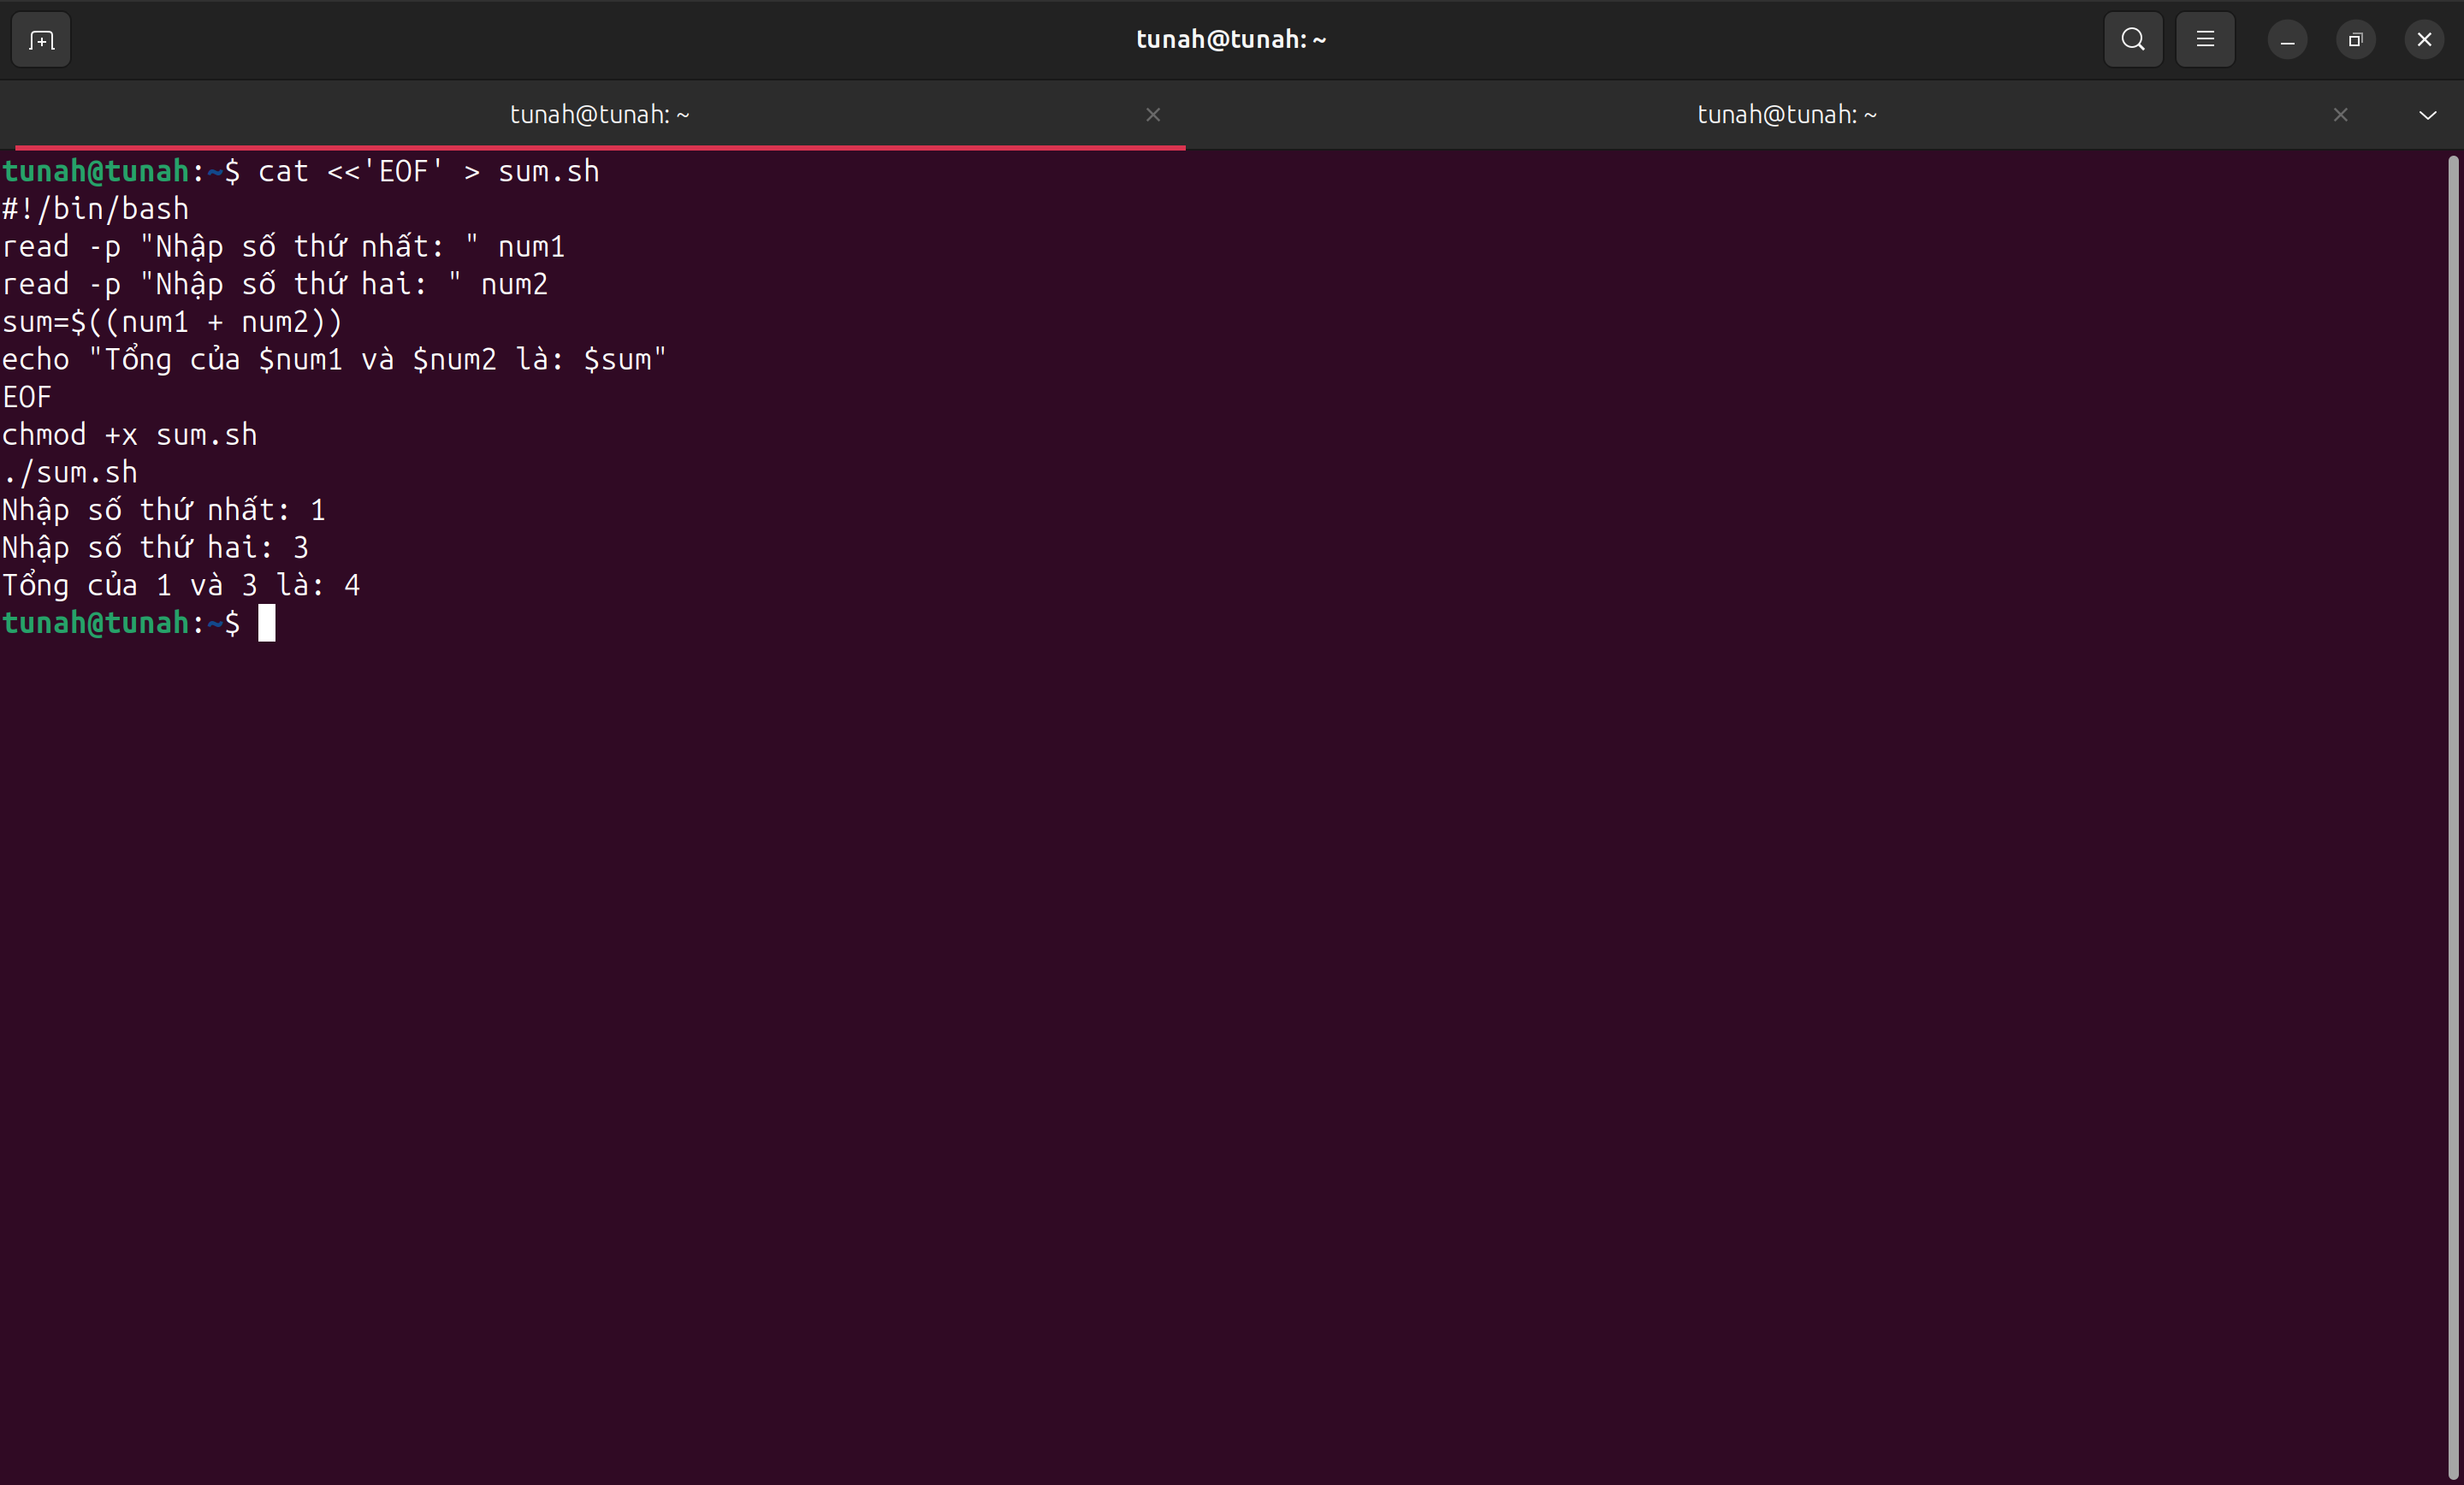
\includegraphics[width=\textwidth]{07/sum-script.png}
        \caption{Tính tổng 2 số}
    \end{subfigure}
    \caption{Các thao tác cơ bản trong Bash Script}
\end{figure}

\subsection{Lệnh điều kiện và Vòng lặp}

\textbf{Cách thực hiện:}
- \texttt{check\_file.sh}: Nhận tên file, dùng \texttt{if [ -f ]} để kiểm tra sự tồn tại.
- \texttt{list\_files.sh}: Chạy lệnh \texttt{ls -la} trong script.
- \texttt{loop\_numbers.sh} \& \texttt{100.sh}: Dùng vòng lặp \texttt{for i in \{1..10\}} để in số.

\begin{lstlisting}[language=bash]
# Chay thu script kiem tra ton tai
./check_file.sh

# Chay thu vong lap in so tu 1 den 100
./loop_numbers_100.sh
\end{lstlisting}

\textbf{Kết quả:}
Hệ thống rẽ nhánh luồng xử lý tùy theo file có tồn tại hay không. Vòng lặp for hoạt động trơn tru từ 1 đến 100.

\begin{figure}[H]
    \centering
    \begin{subfigure}[b]{0.45\textwidth}
        \centering
        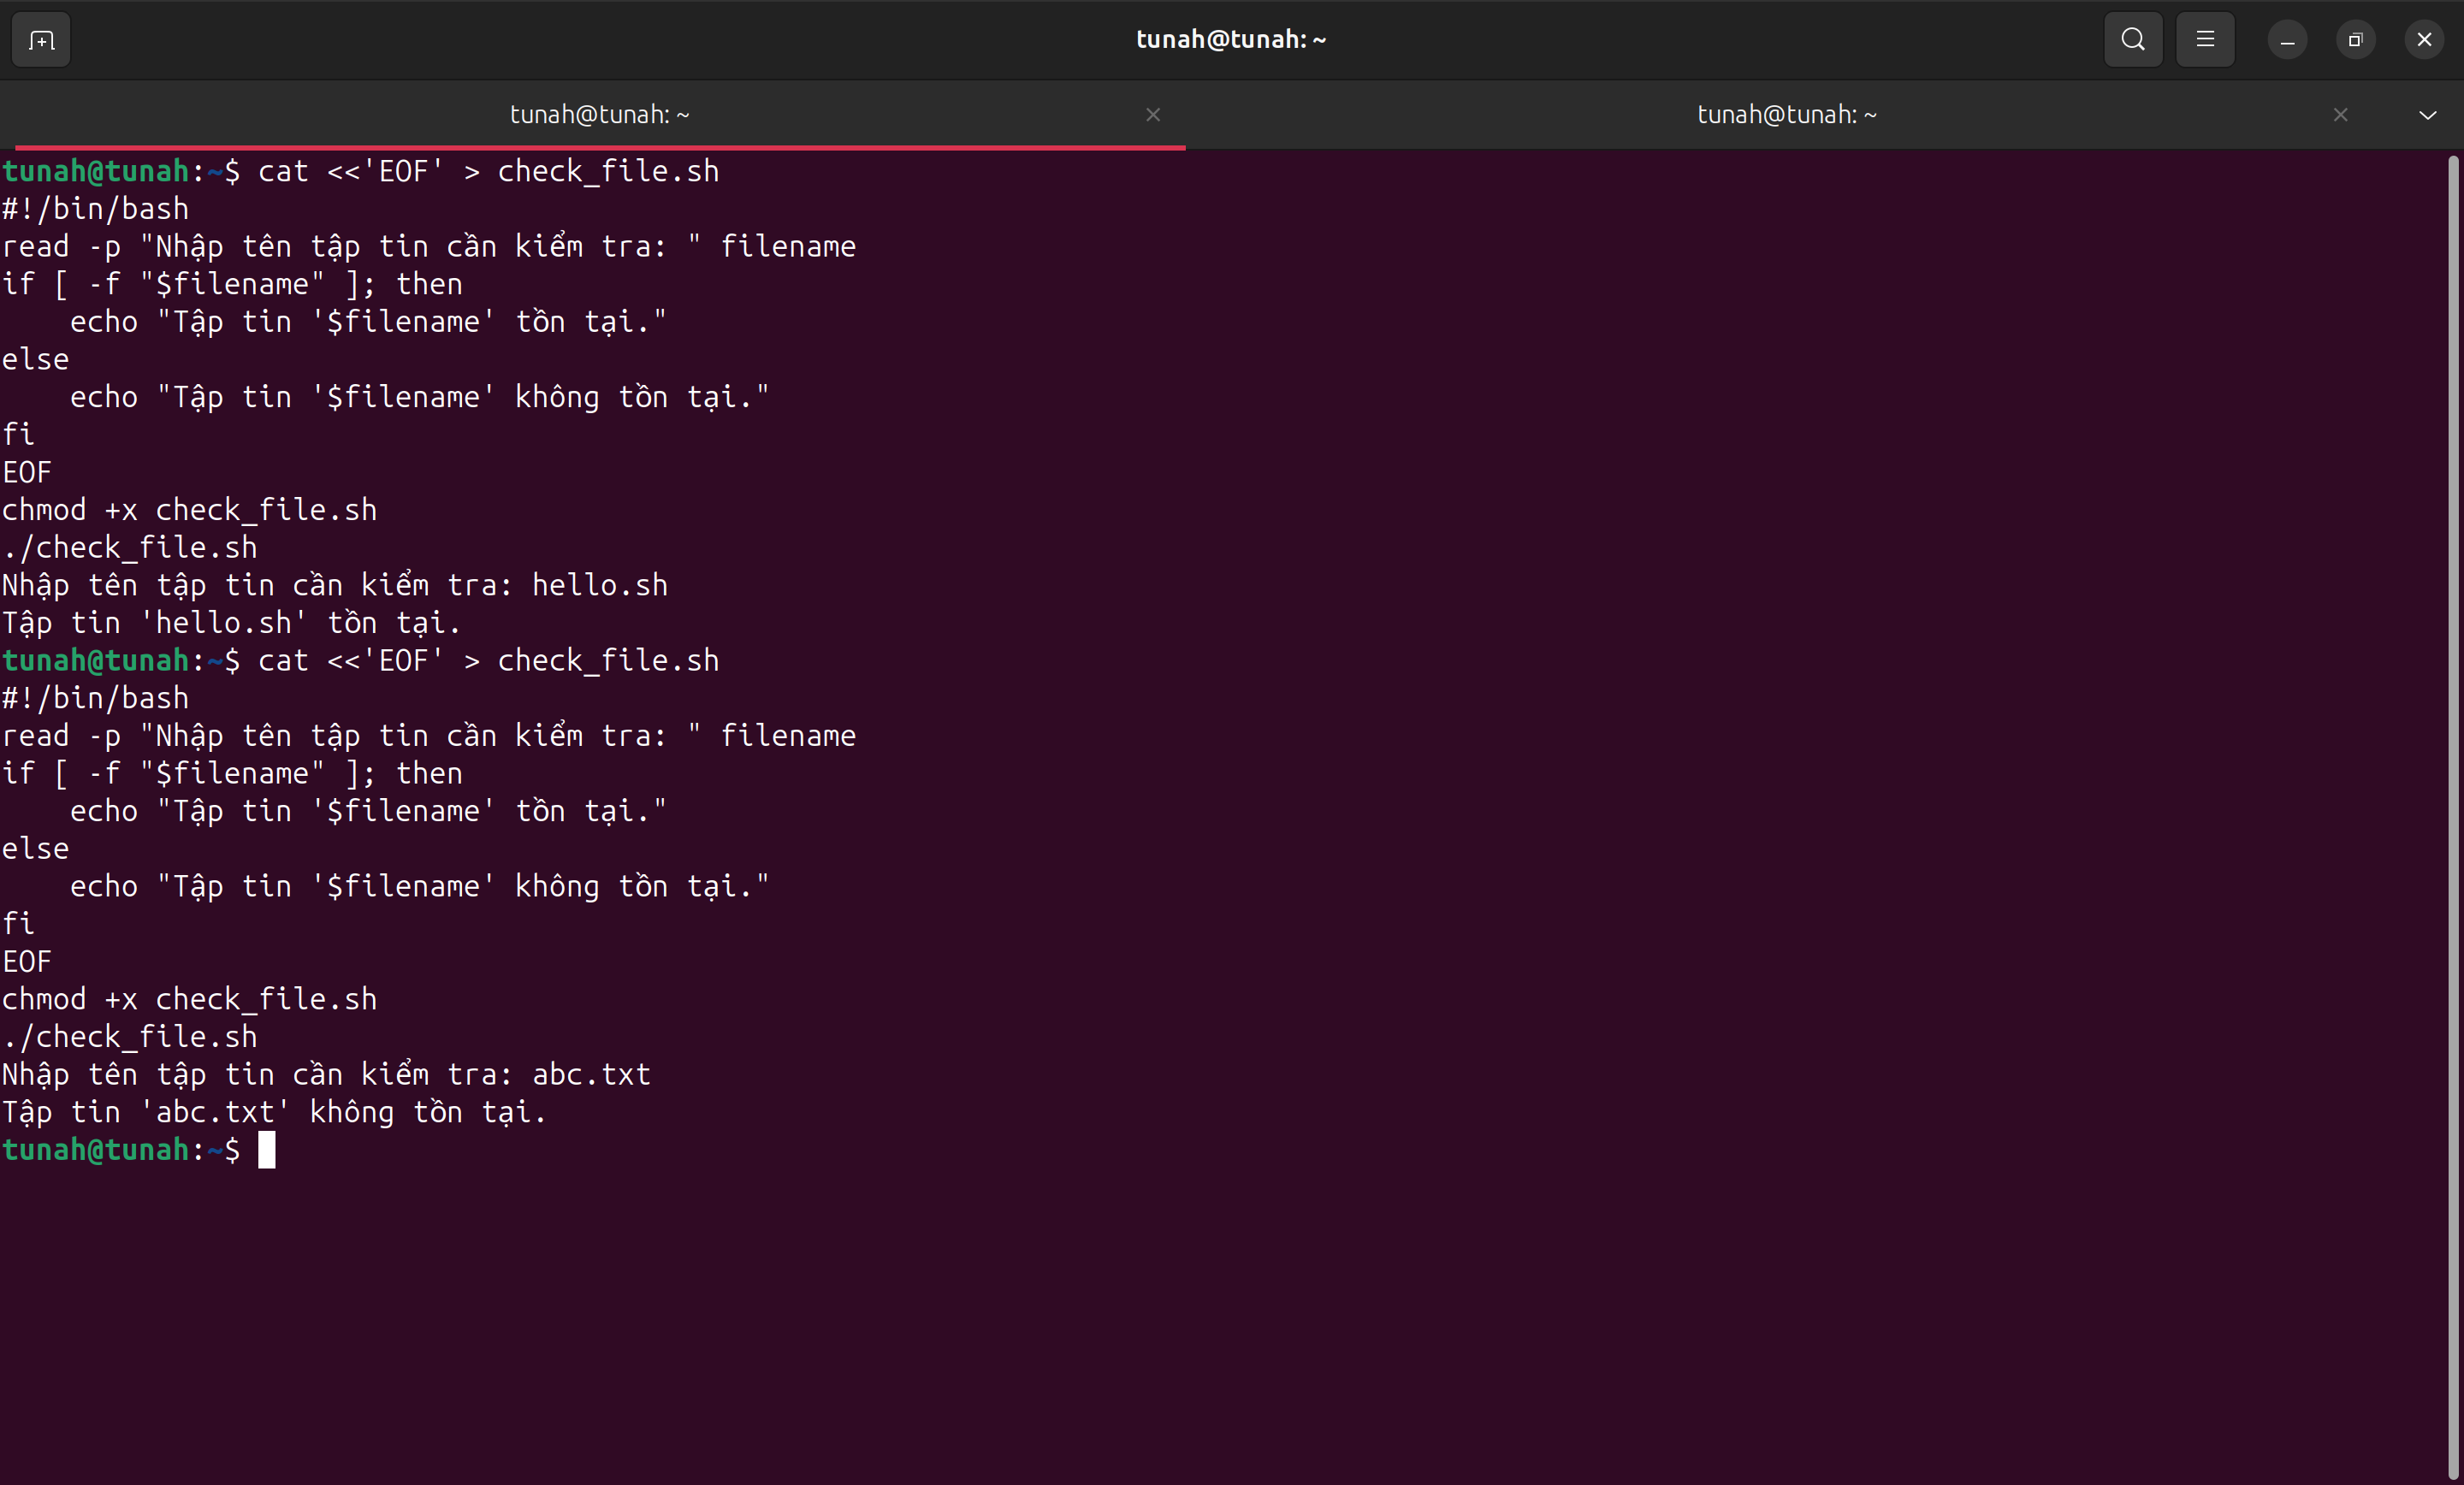
\includegraphics[width=\textwidth]{07/check-file-script.png}
        \caption{Kiểm tra sự tồn tại của file}
    \end{subfigure}
    \hfill
    \begin{subfigure}[b]{0.45\textwidth}
        \centering
        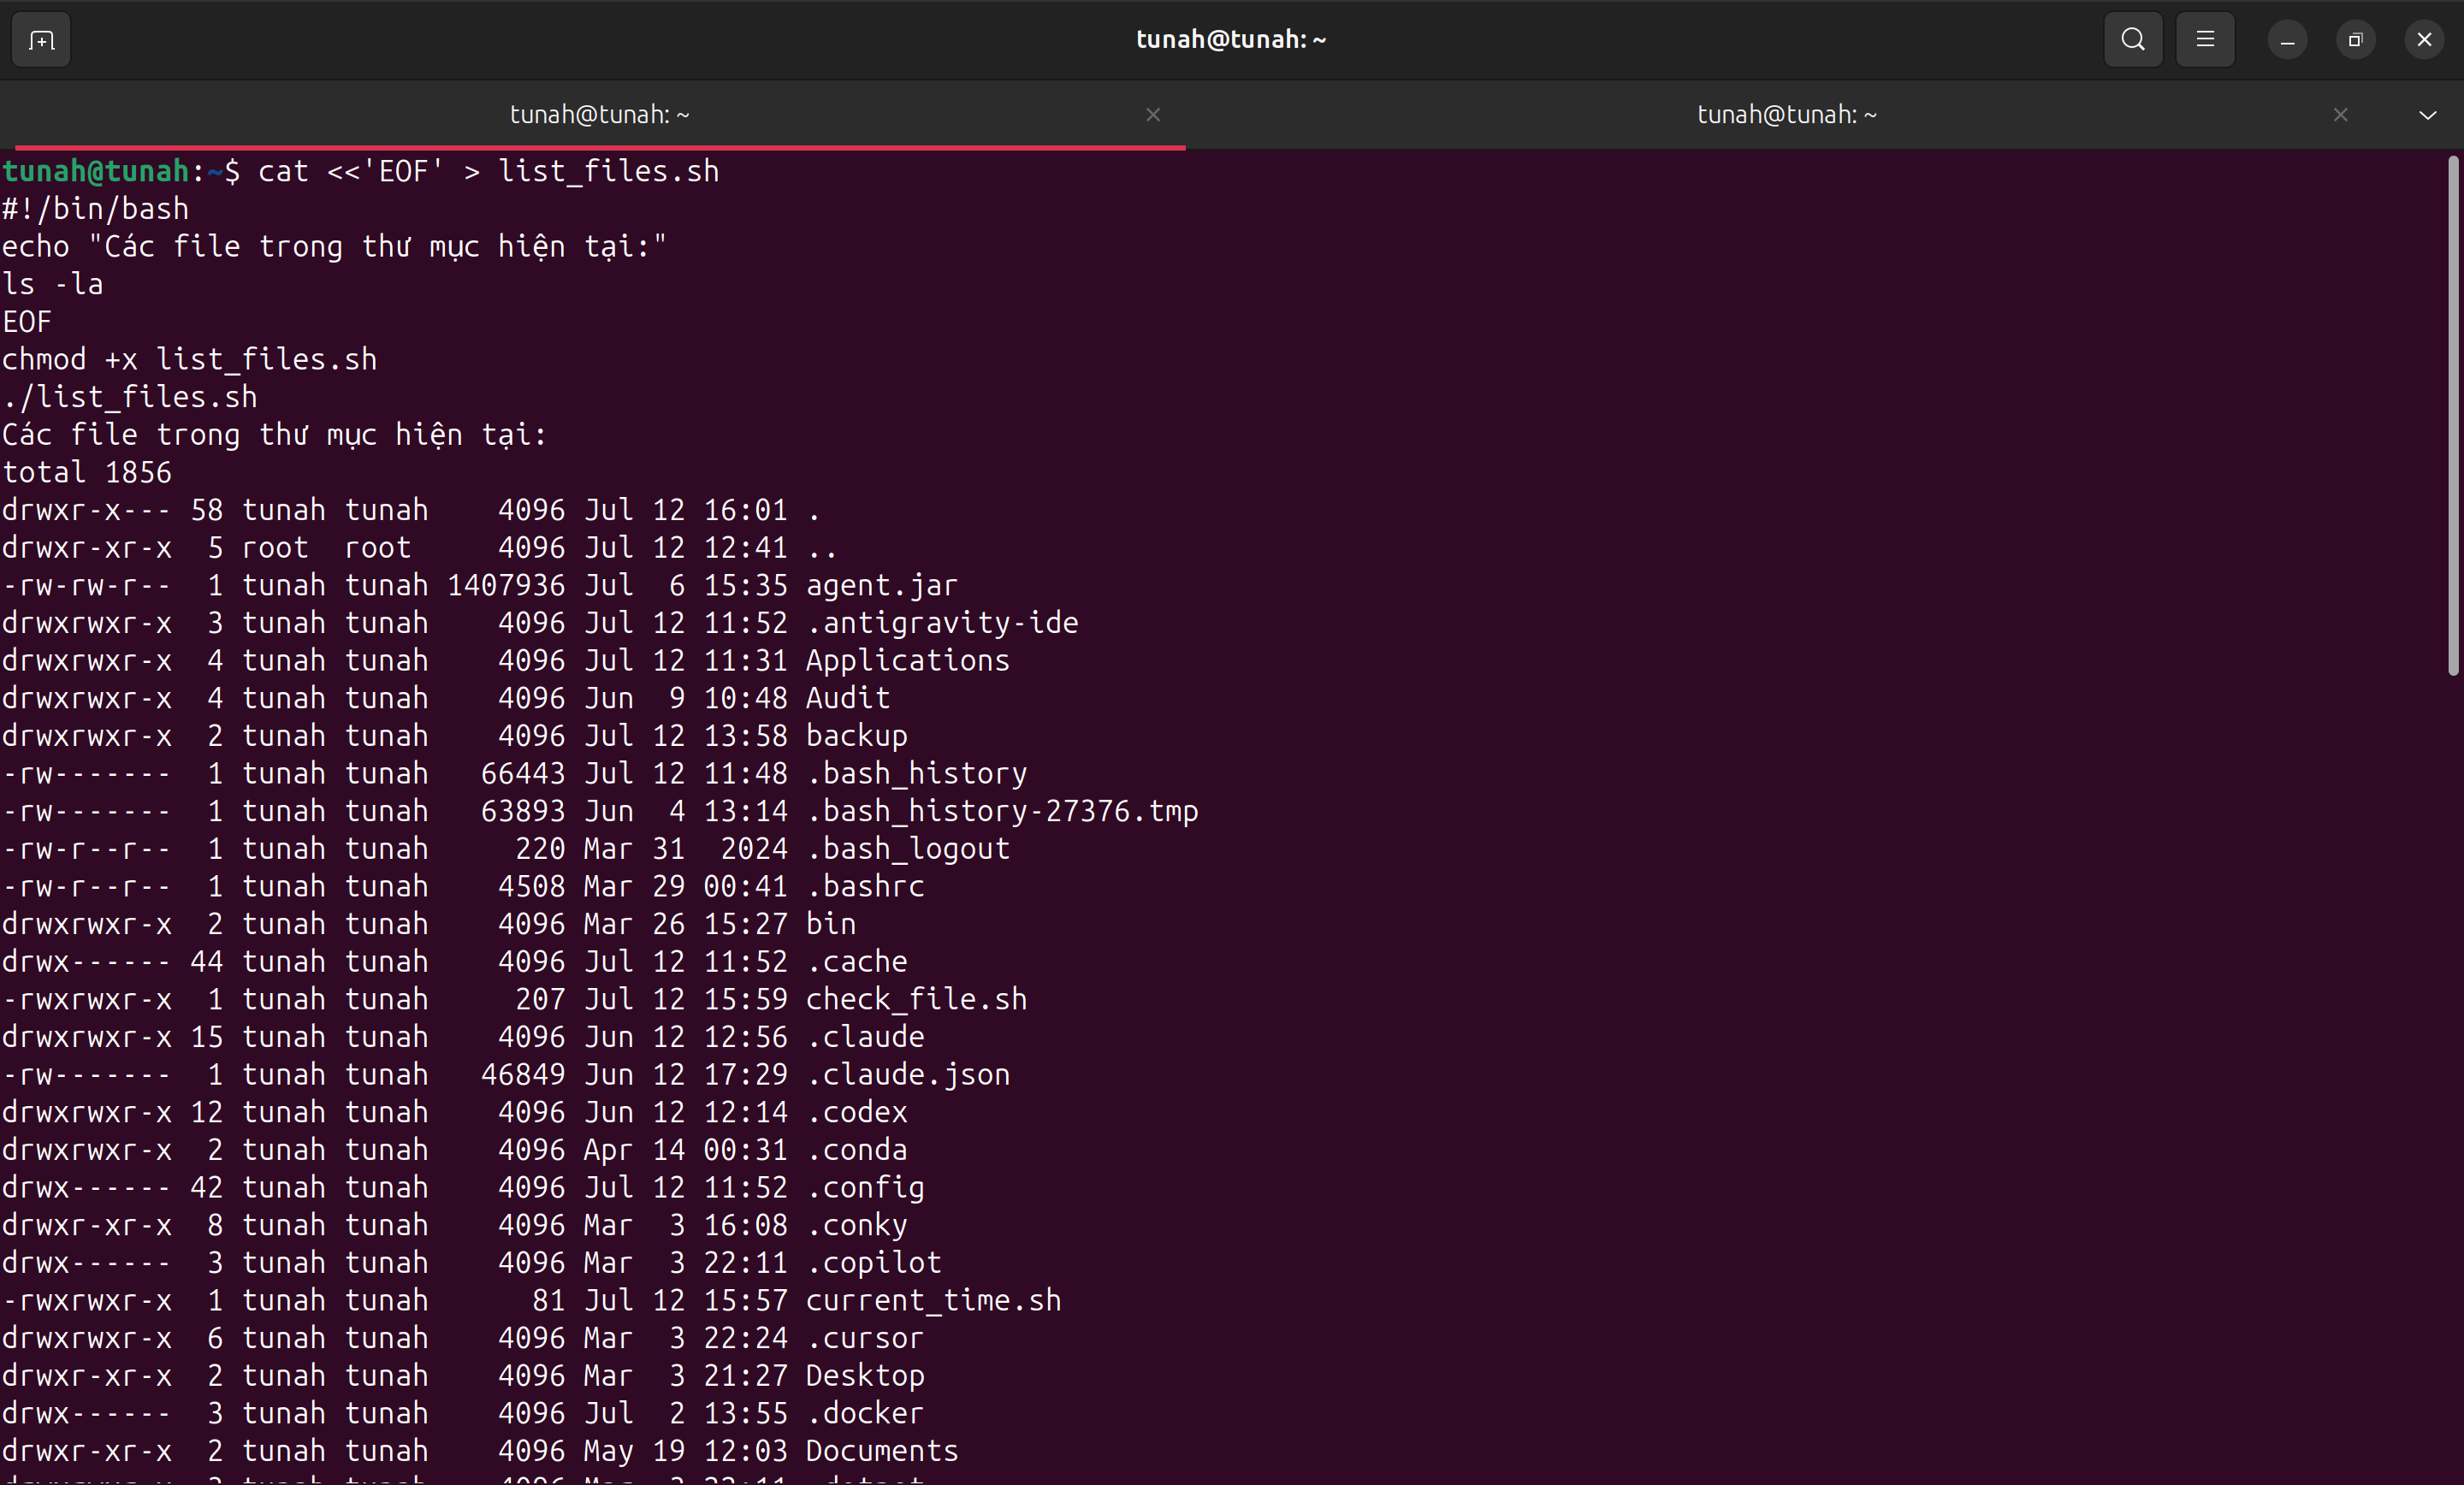
\includegraphics[width=\textwidth]{07/list-files-script.png}
        \caption{Script liệt kê file}
    \end{subfigure}
    
    \vspace{0.5cm}
    \begin{subfigure}[b]{0.45\textwidth}
        \centering
        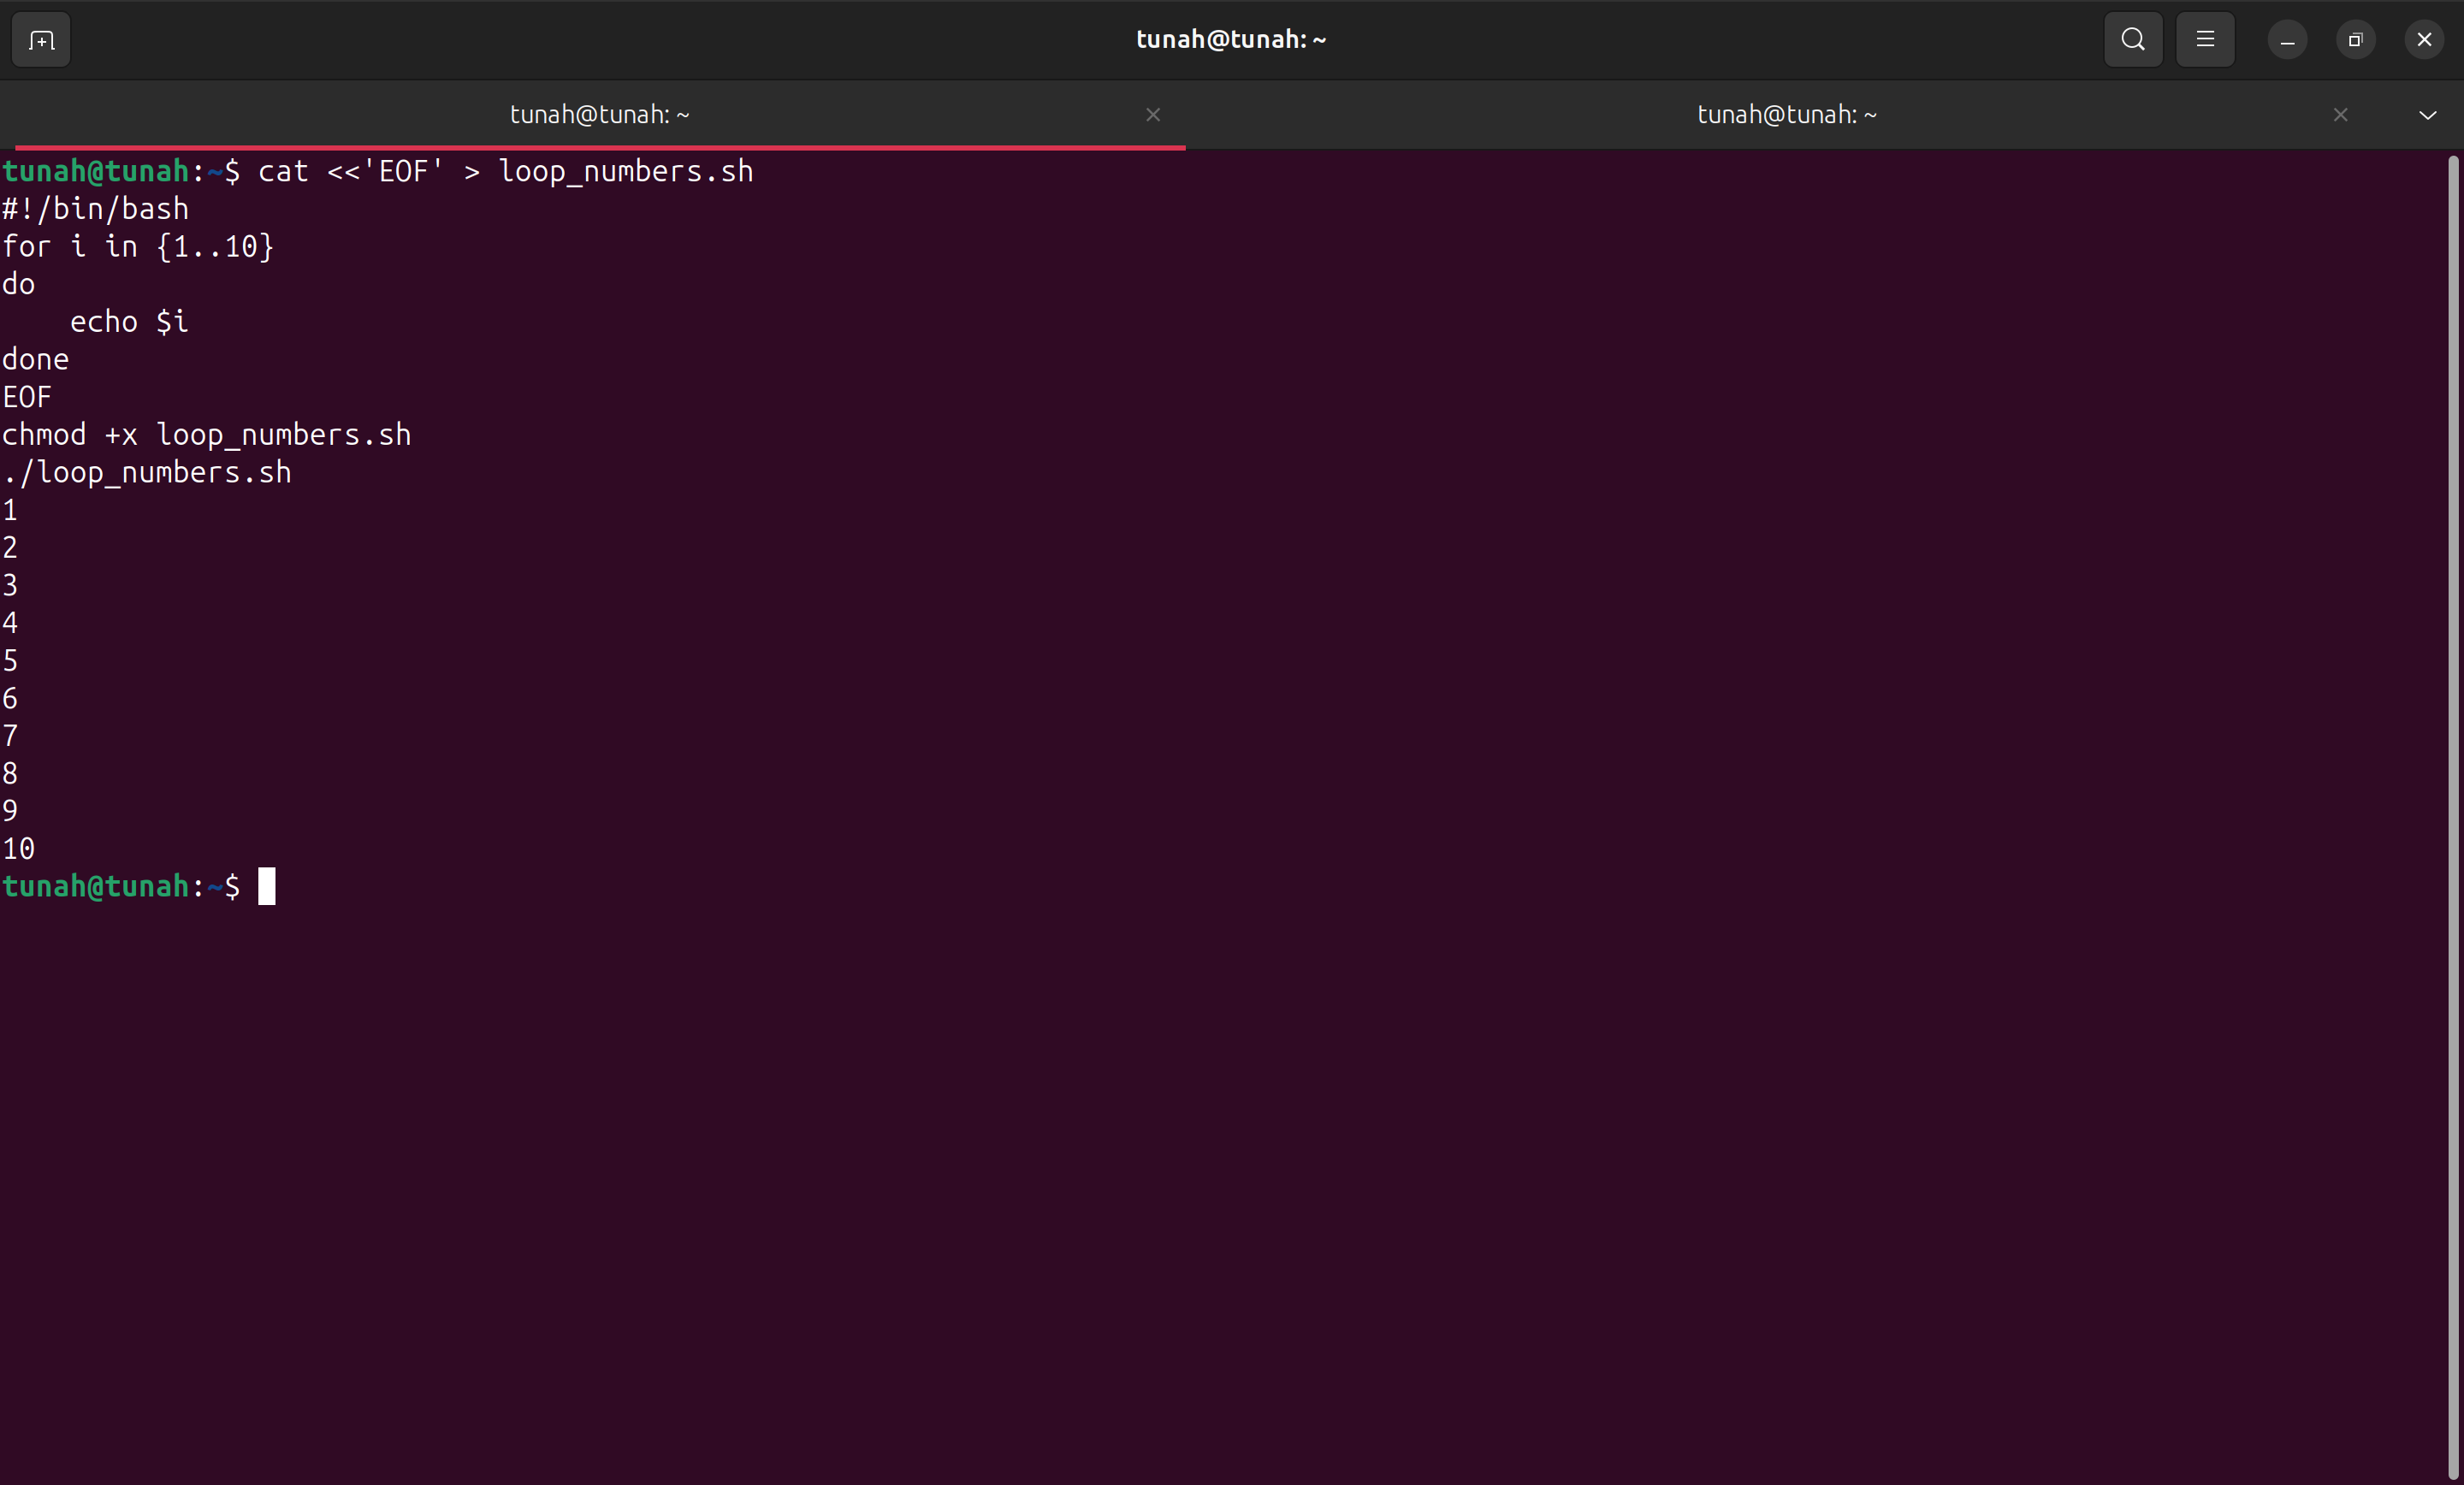
\includegraphics[width=\textwidth]{07/loop-1-to-10.png}
        \caption{Vòng lặp 1-10}
    \end{subfigure}
    \hfill
    \begin{subfigure}[b]{0.45\textwidth}
        \centering
        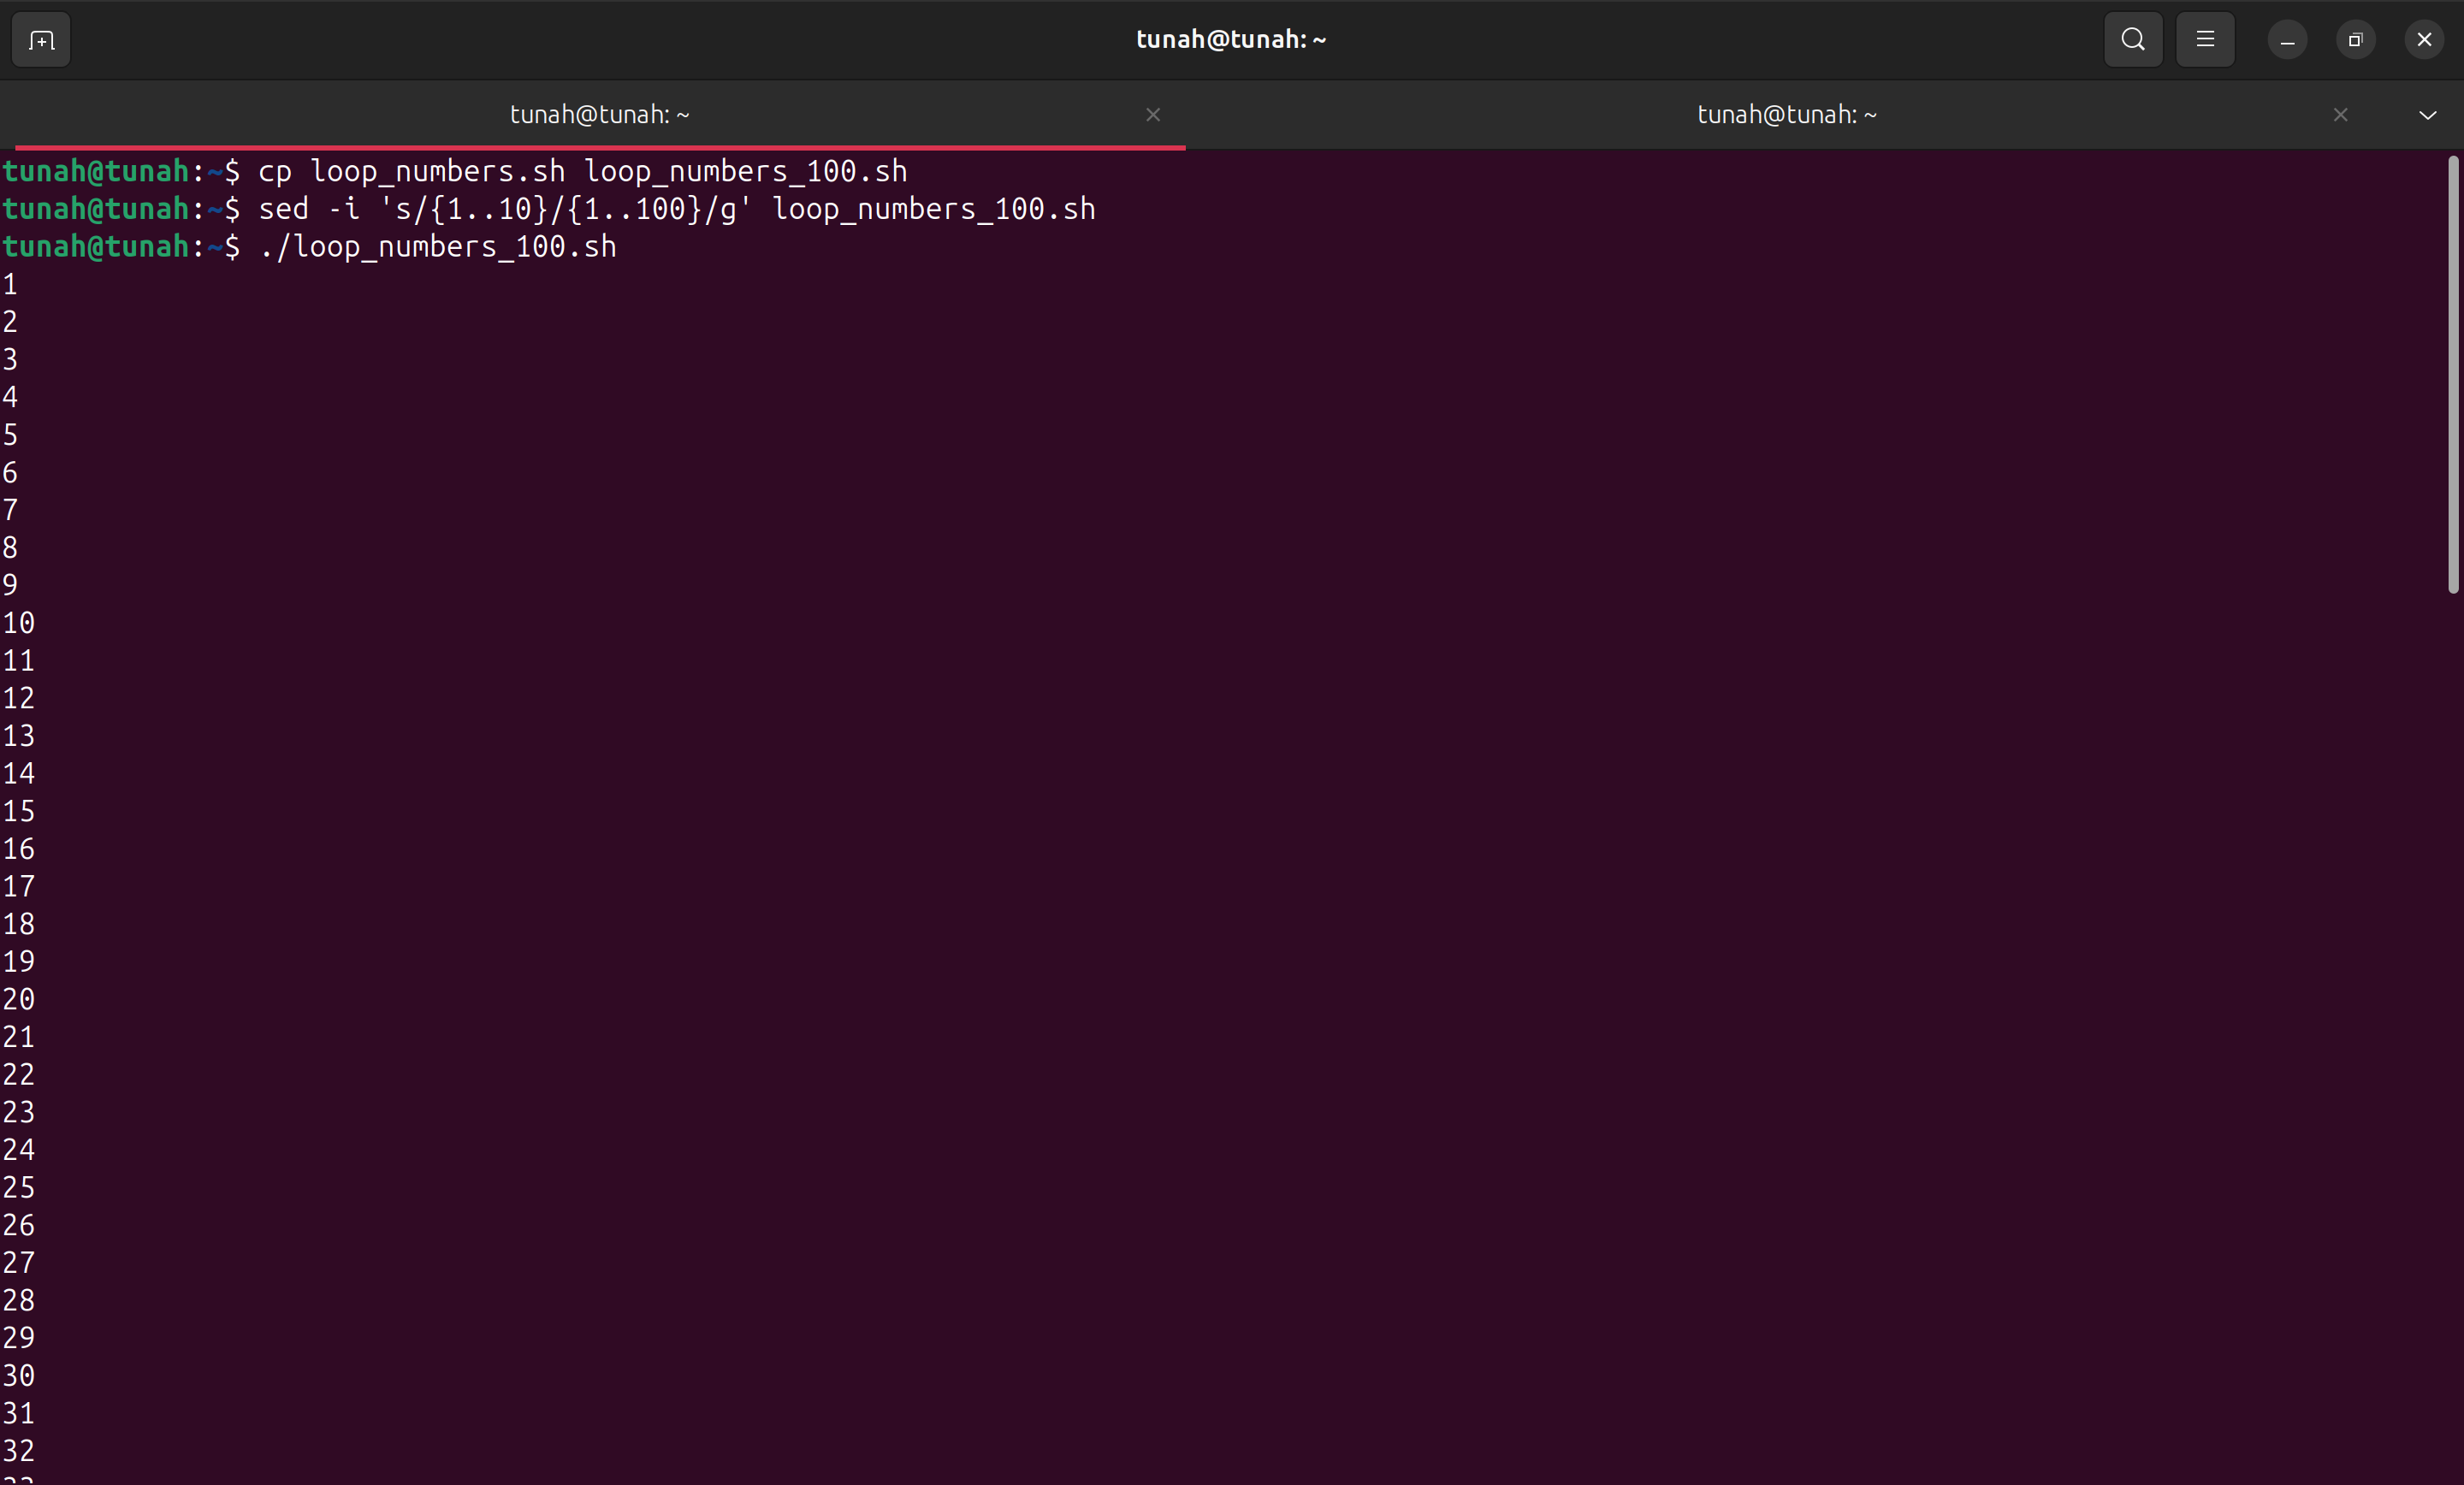
\includegraphics[width=\textwidth]{07/loop-1-to-100.png}
        \caption{Vòng lặp 1-100}
    \end{subfigure}
    \caption{Điều khiển luồng trong Bash}
\end{figure}

\subsection{Xử lý File nâng cao (Đếm dòng, Backup tự động)}

\textbf{Cách thực hiện:}
- \texttt{count\_lines.sh}: Sử dụng lệnh \texttt{wc -l} trong kịch bản để đếm số dòng của file chỉ định.
- \texttt{backup\_file.sh}: Sao lưu file thành bản sao mới có gắn nhãn thời gian hiện tại (\texttt{\%Y\%m\%d\_\%H\%M\%S}).

\begin{lstlisting}[language=bash]
./count_lines.sh
./backup_file.sh
\end{lstlisting}

\textbf{Kết quả:}
Tạo bản sao lưu không lo trùng tên nhờ tích hợp biến ngày giờ hệ thống động.

\begin{figure}[H]
    \centering
    \begin{subfigure}[b]{0.48\textwidth}
        \centering
        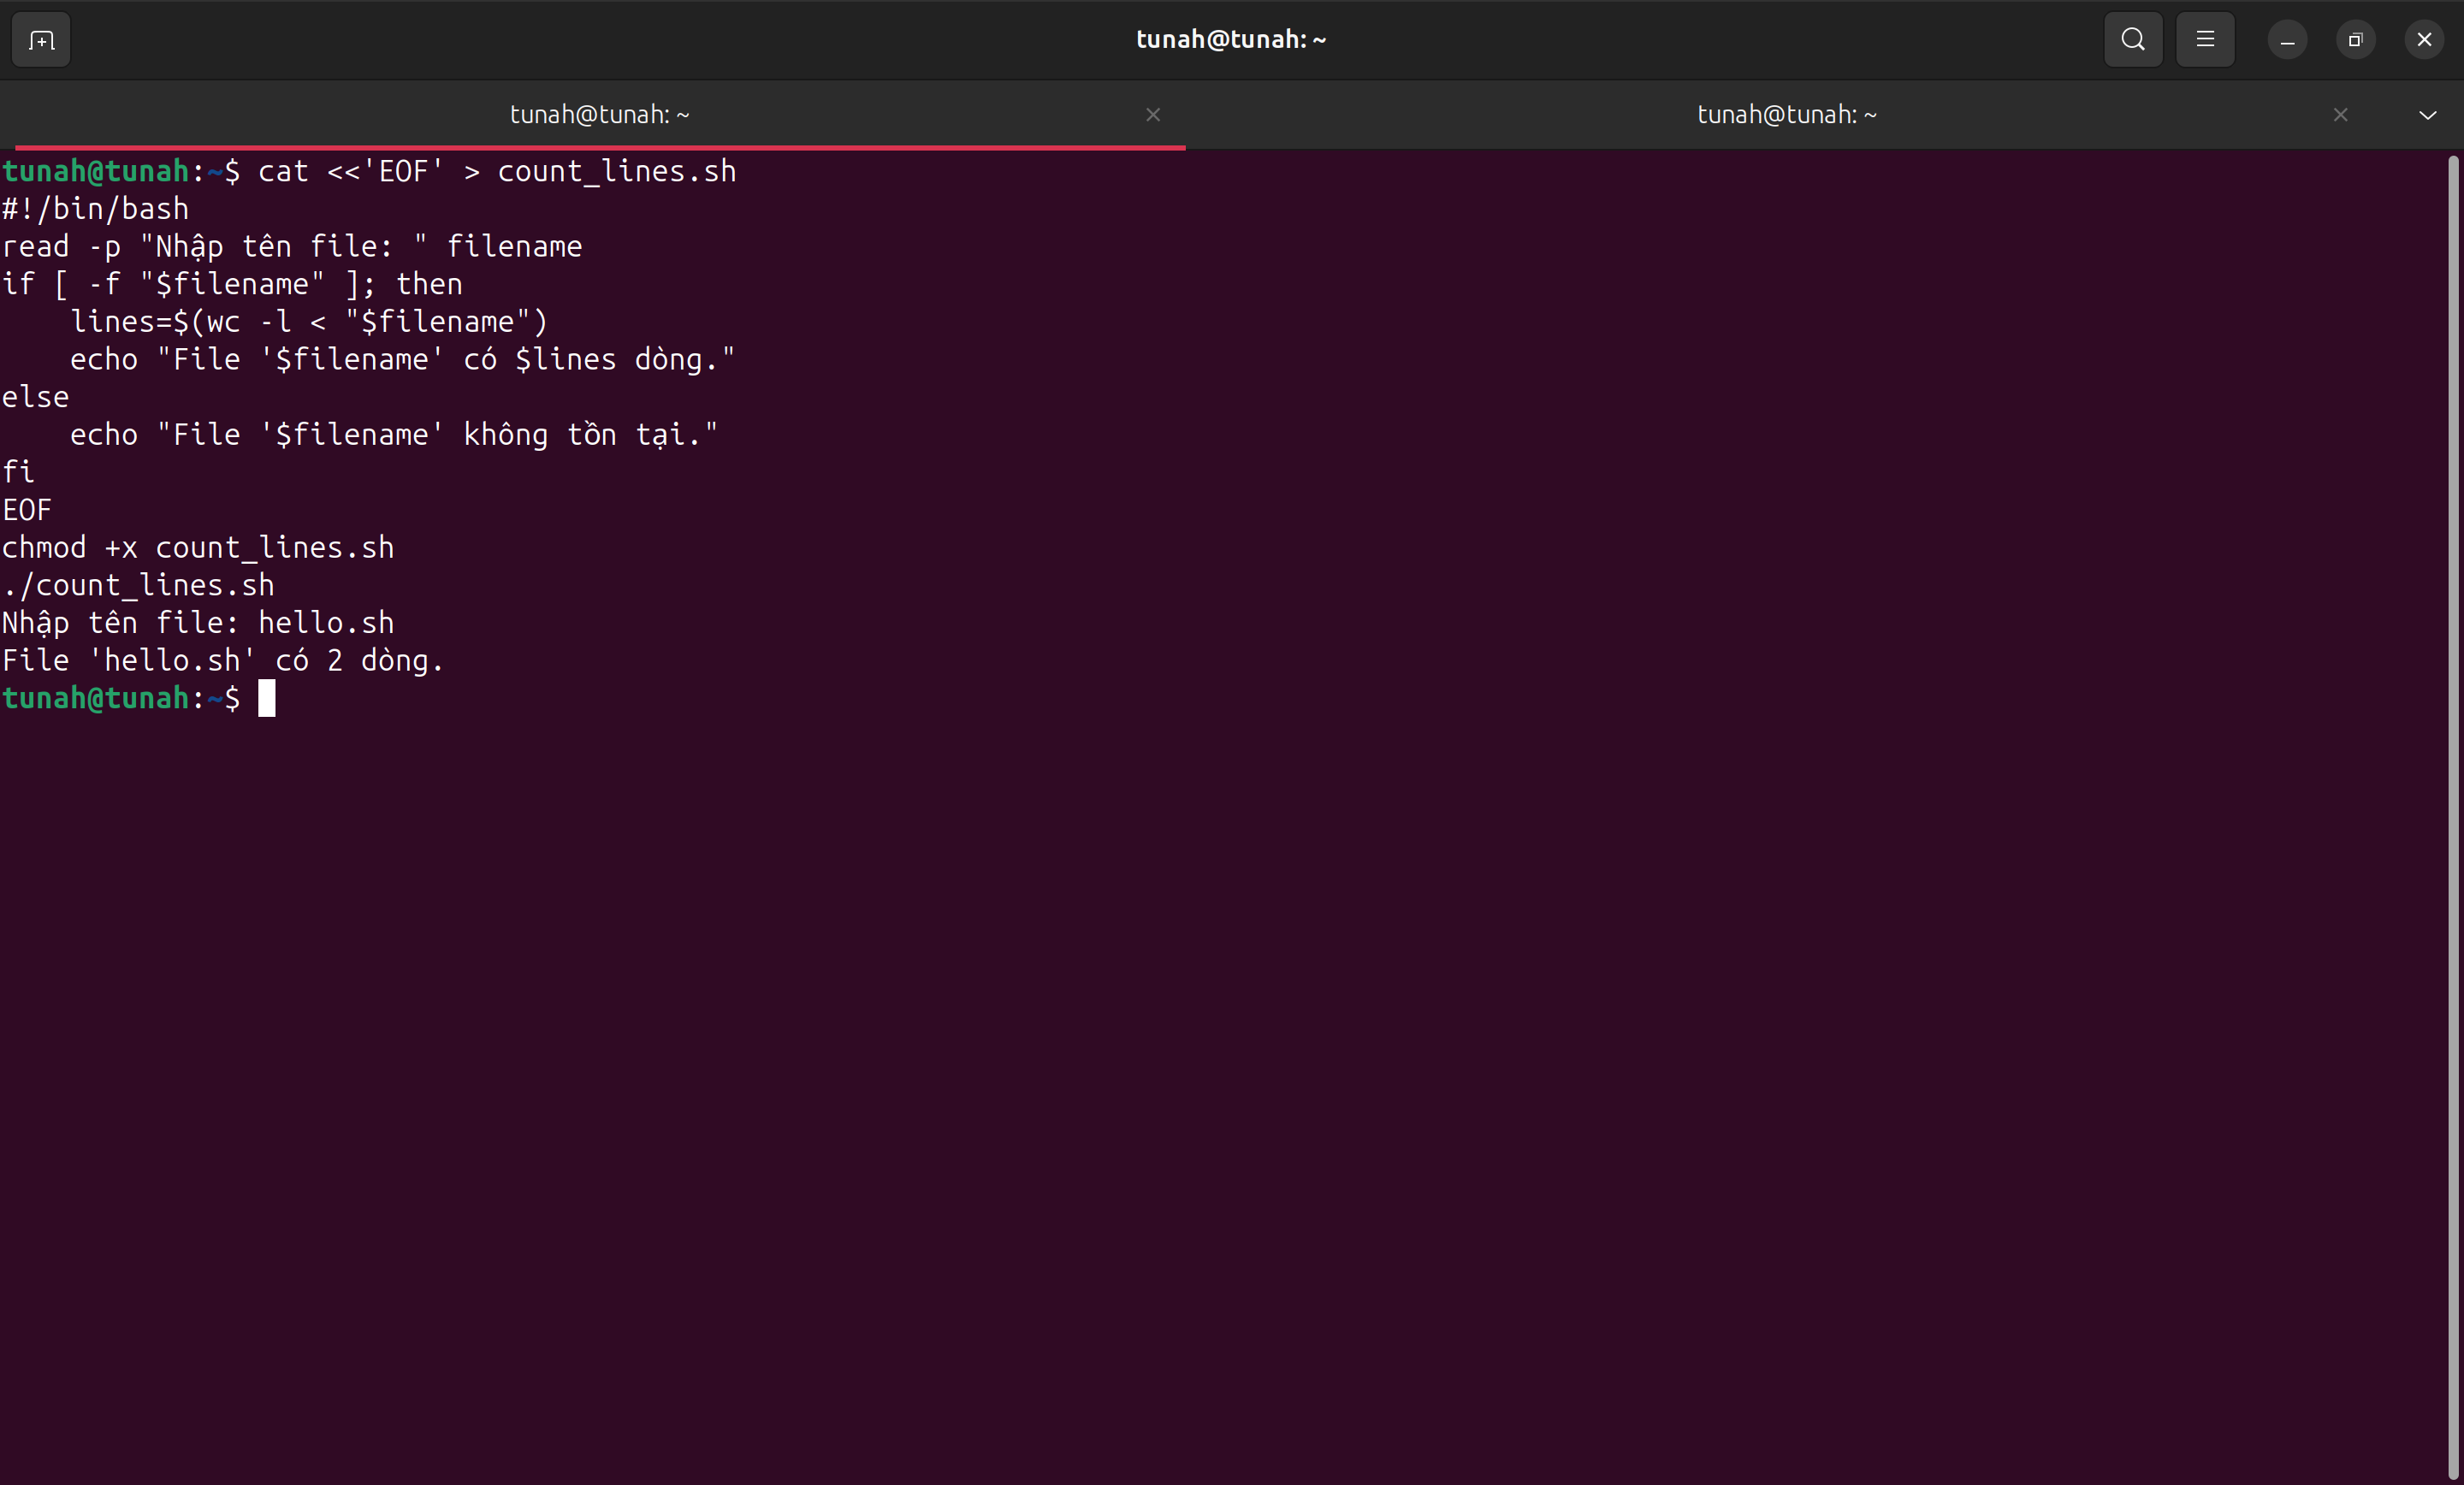
\includegraphics[width=\textwidth]{07/count-lines-script.png}
        \caption{Script đếm số dòng file}
    \end{subfigure}
    \hfill
    \begin{subfigure}[b]{0.48\textwidth}
        \centering
        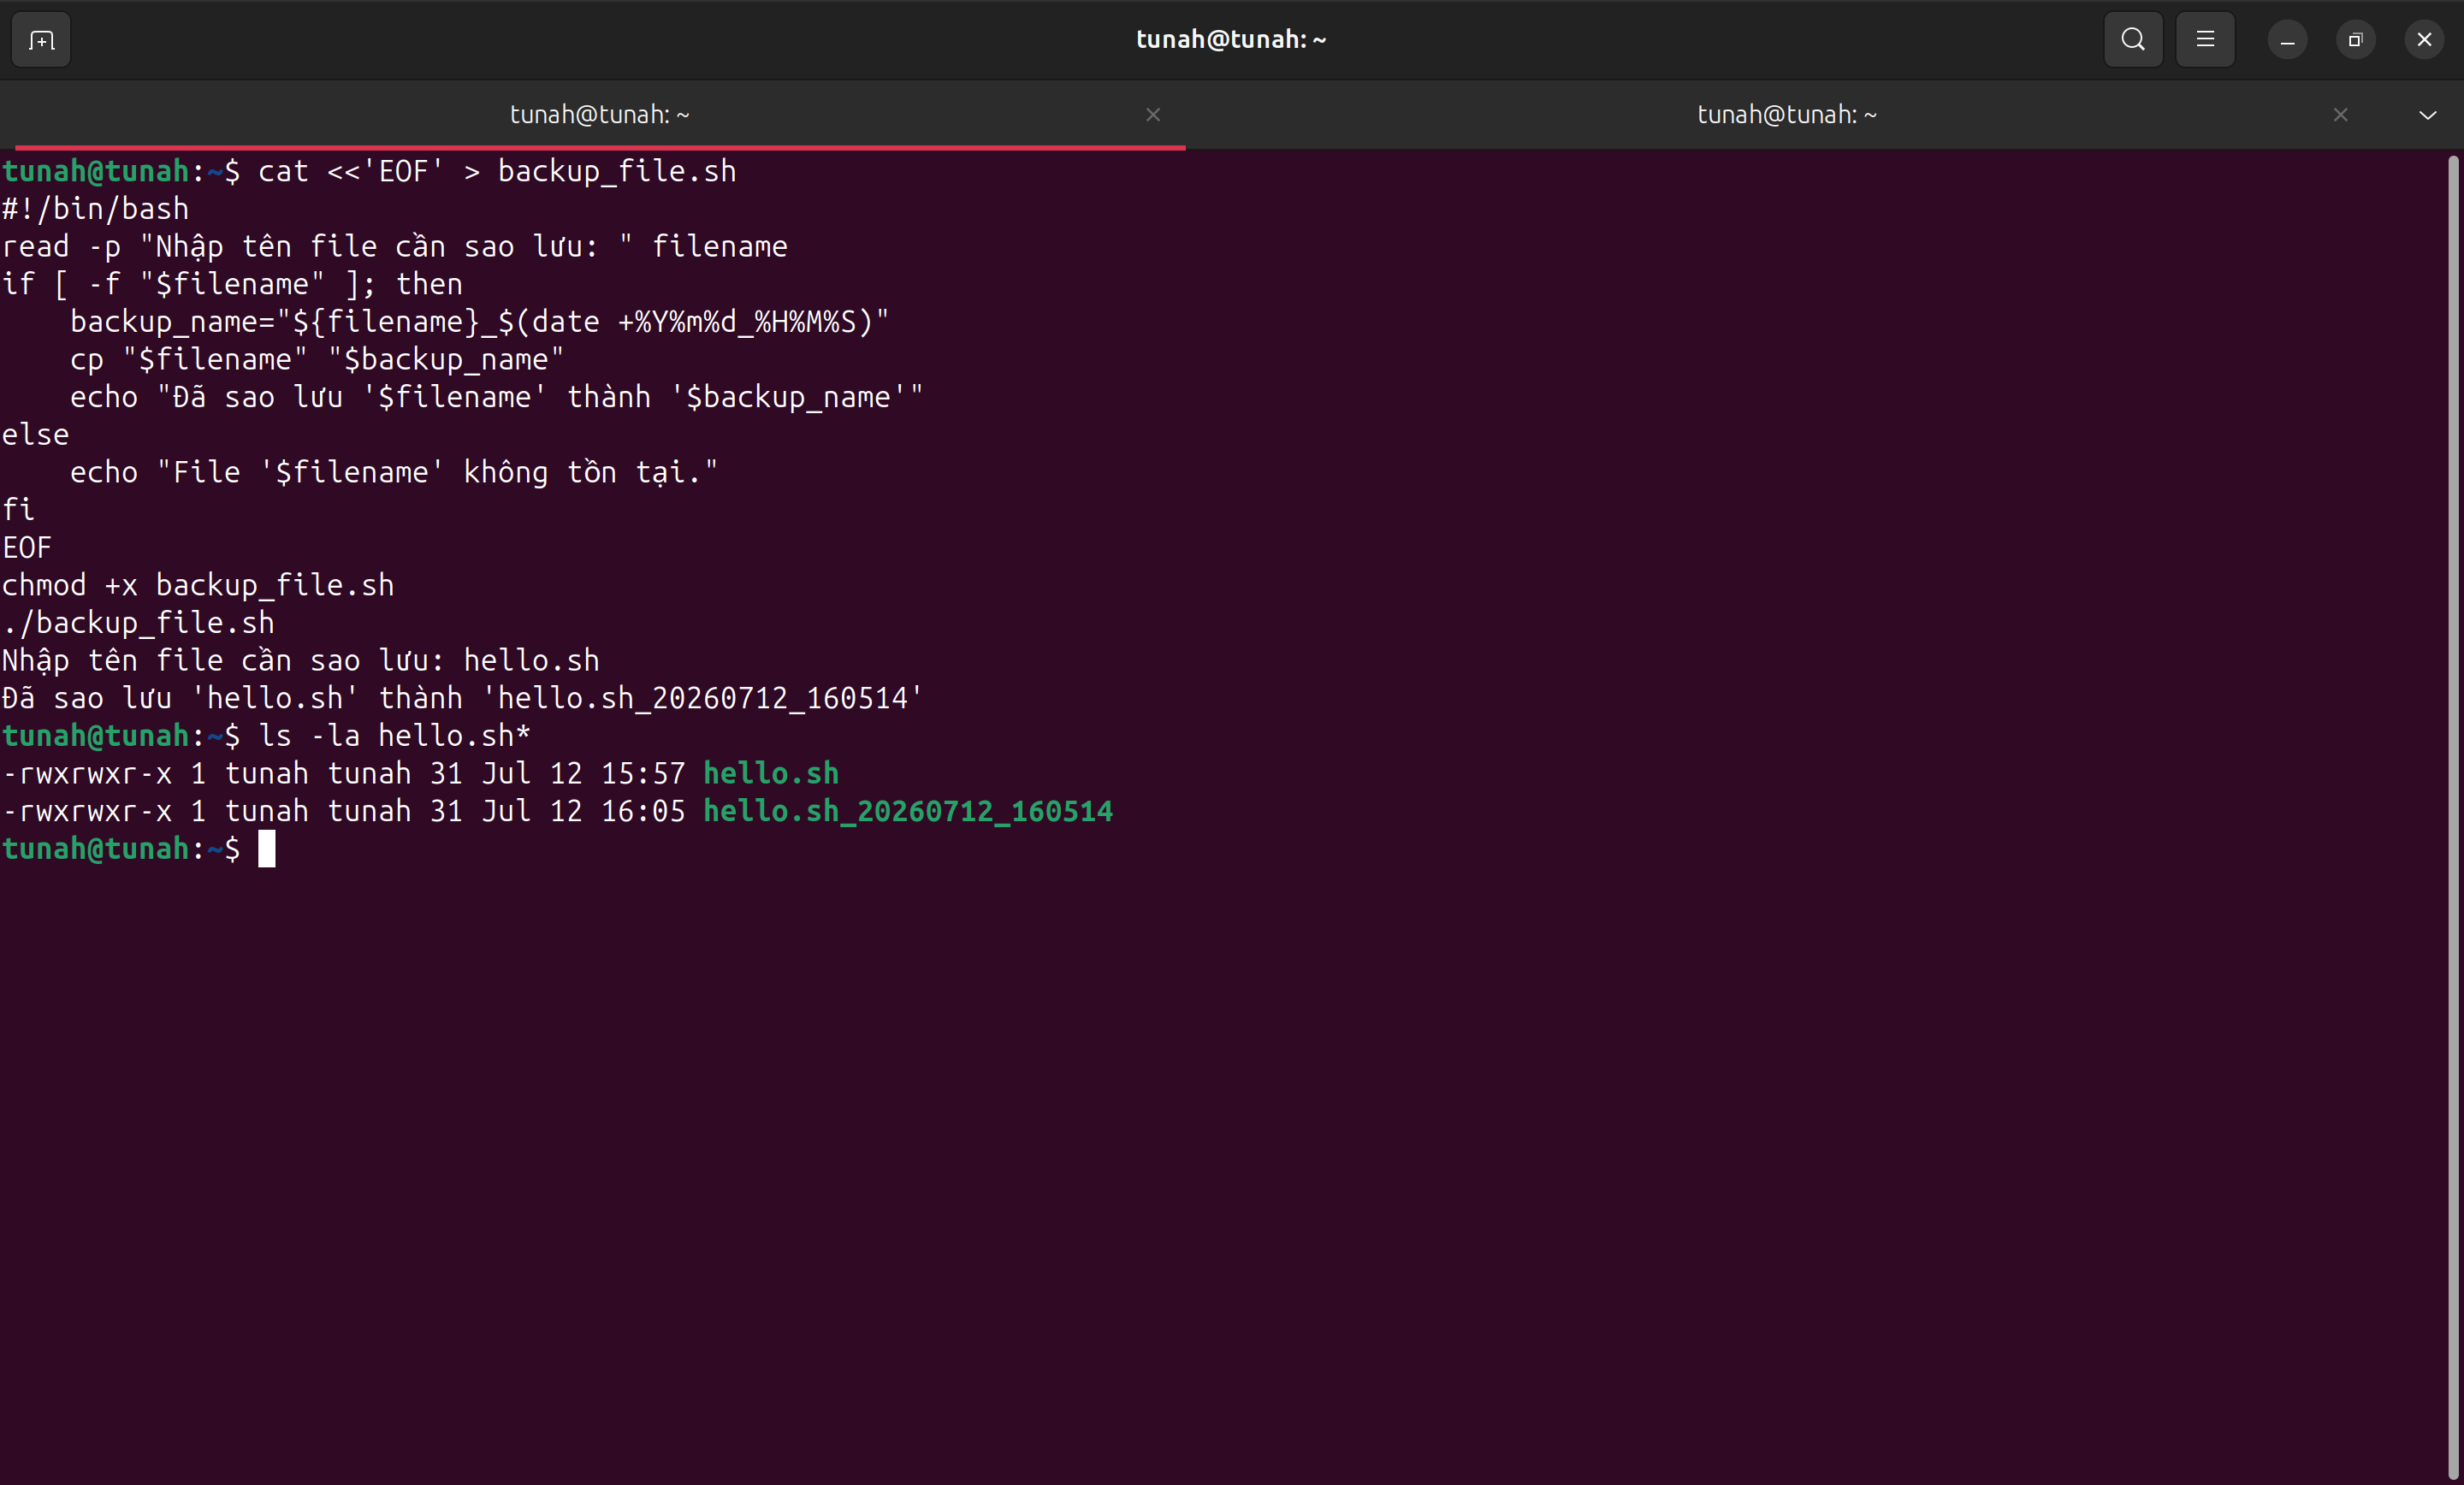
\includegraphics[width=\textwidth]{07/backup-file-script.png}
        \caption{Backup với định dạng datetime}
    \end{subfigure}
    \caption{Ứng dụng xử lý file bằng Script}
\end{figure}

\subsection{Tự động hóa với Crontab}

\textbf{Cách thực hiện:}
Lập lịch tự động chạy hai tác vụ bằng Cron:
1. Ghi log mỗi 2 phút bằng \texttt{*/2 * * * *}.
2. Sao lưu toàn bộ thư mục \texttt{\textasciitilde/myfolder} vào lúc 2h sáng mỗi ngày bằng \texttt{0 2 * * *}.

\begin{lstlisting}[language=bash]
crontab -e
crontab -l
# Doi sau vai phut va doc log ghi ra
cat ~/output.log
ls -la ~/backup/
\end{lstlisting}

\textbf{Kết quả:}
Hai cronjob đã được thêm vào hệ thống và hoạt động đúng giờ. Dữ liệu được ghi vào \texttt{output.log} tuần tự và thư mục backup được tạo tự động.

\begin{figure}[H]
    \centering
    \begin{subfigure}[b]{0.45\textwidth}
        \centering
        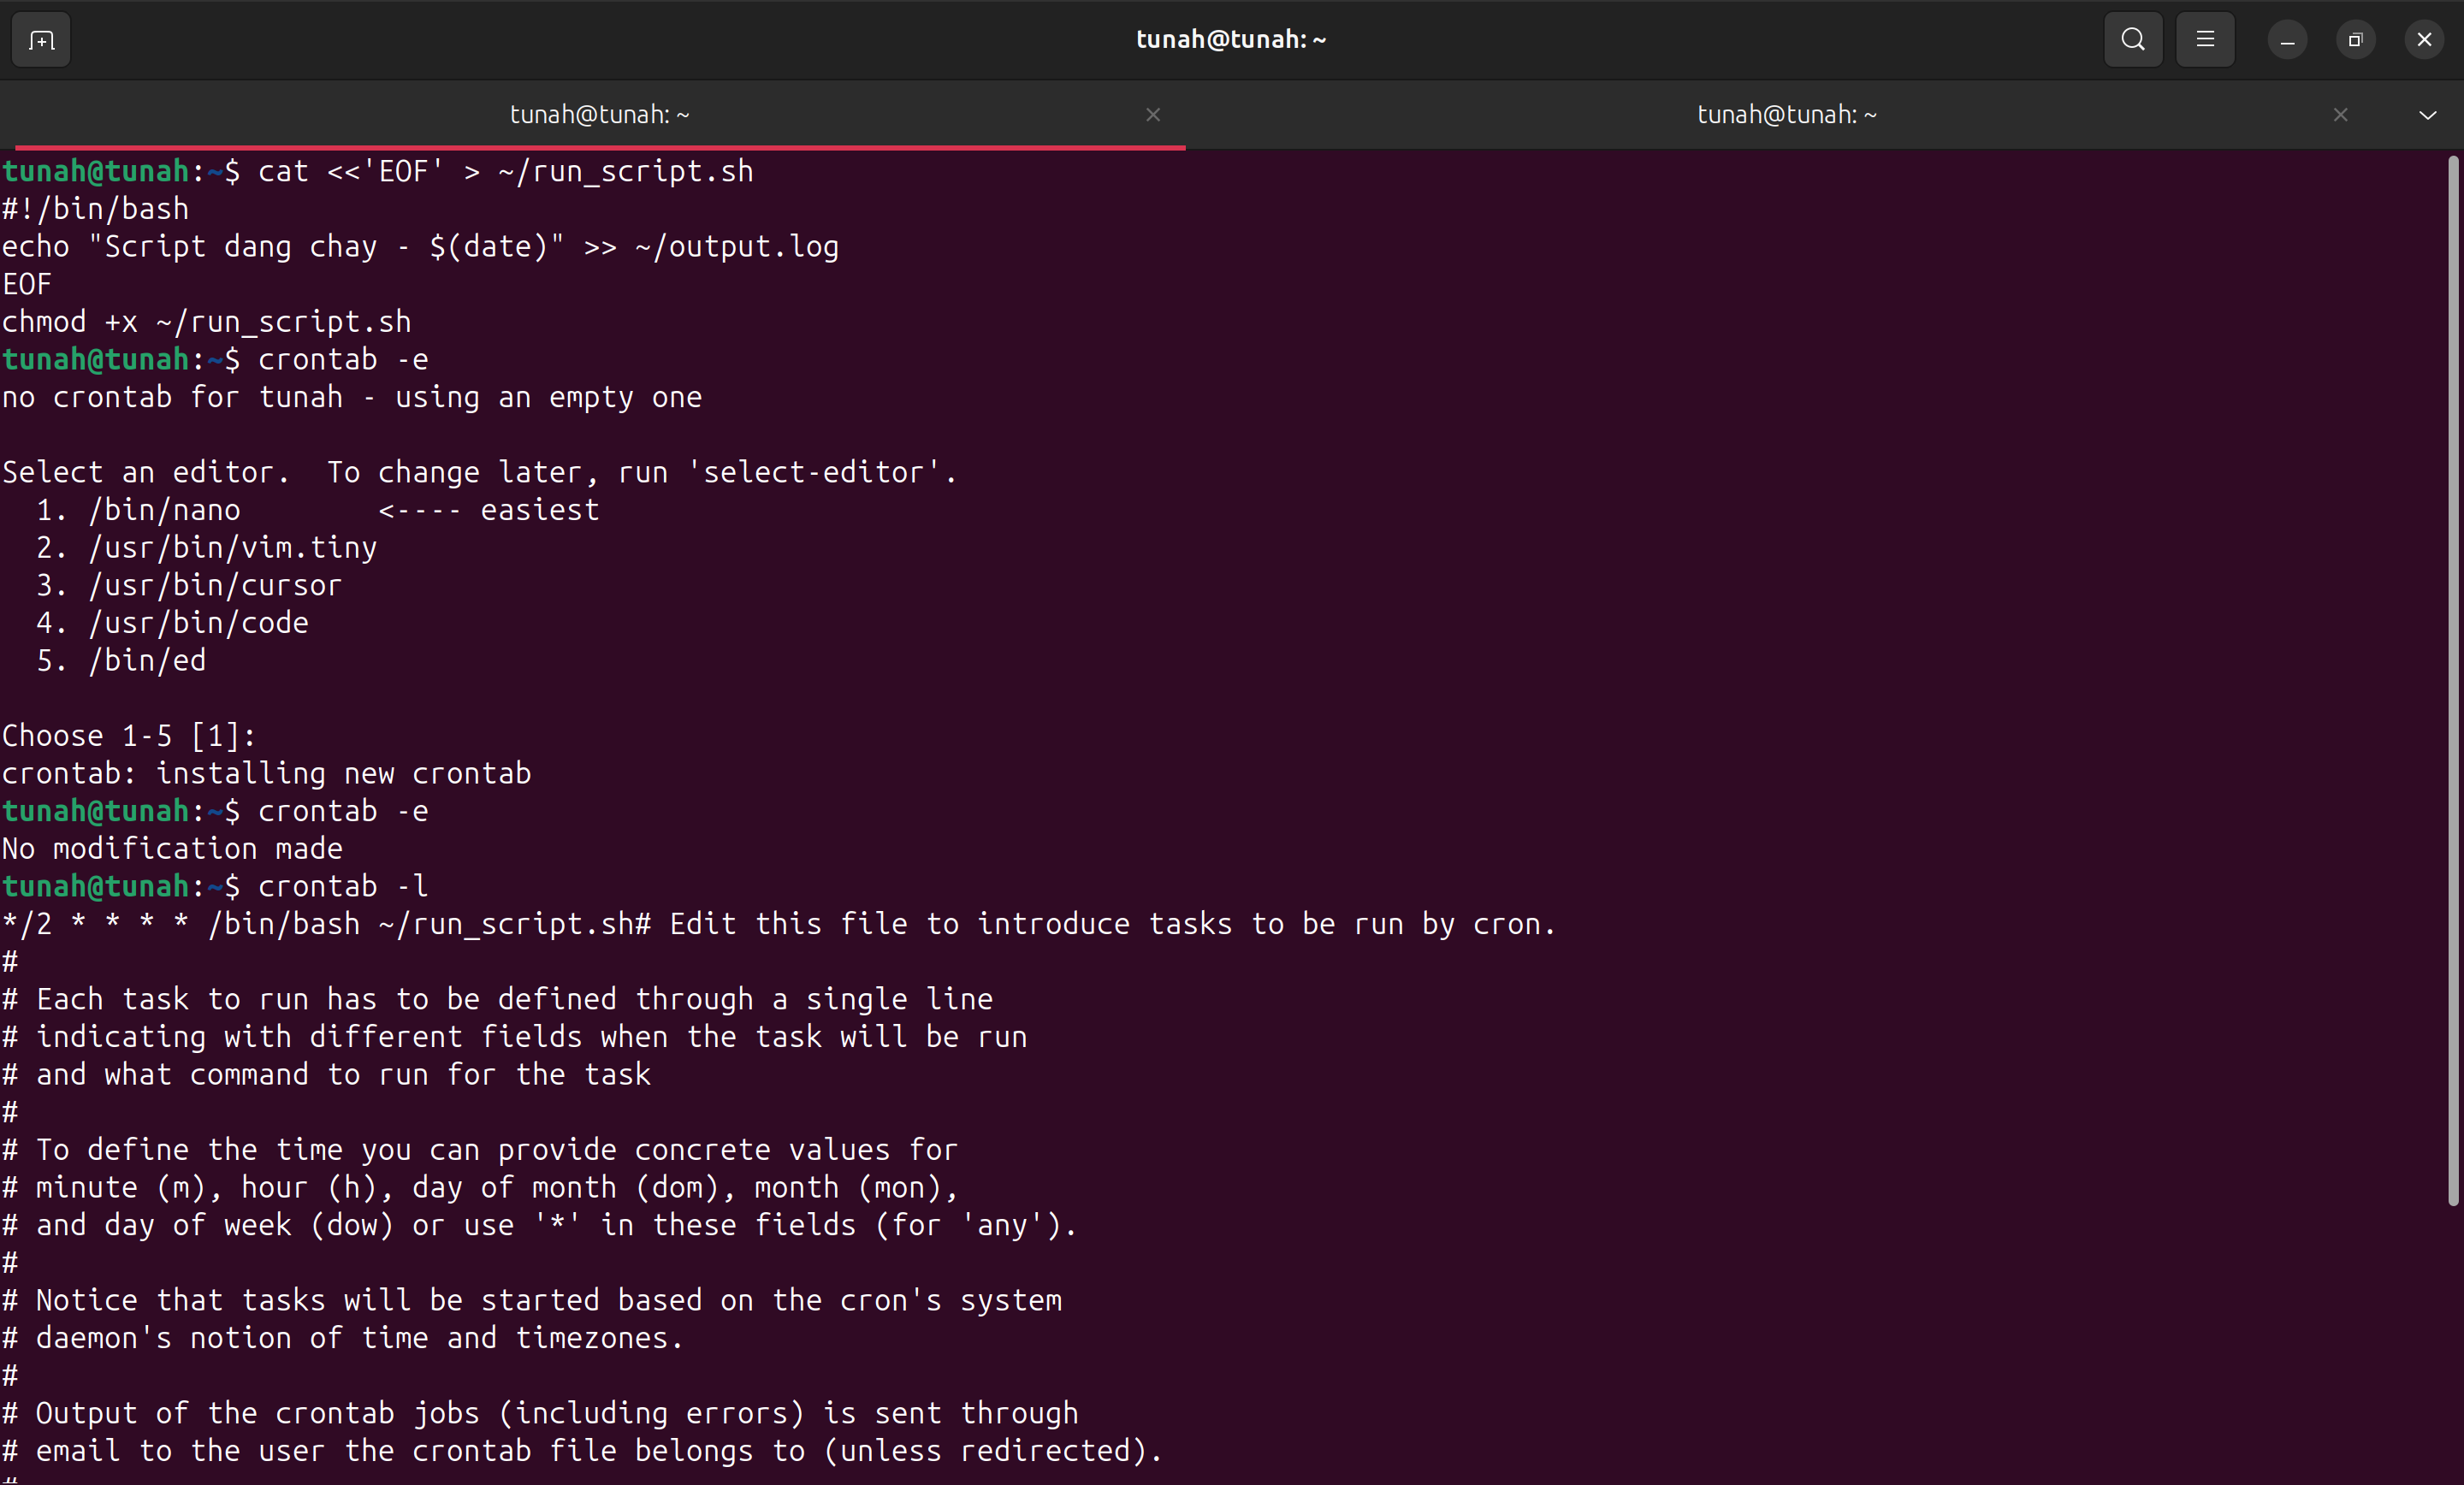
\includegraphics[width=\textwidth]{07/crontab-setup.png}
        \caption{Thiết lập crontab cho log}
    \end{subfigure}
    \hfill
    \begin{subfigure}[b]{0.45\textwidth}
        \centering
        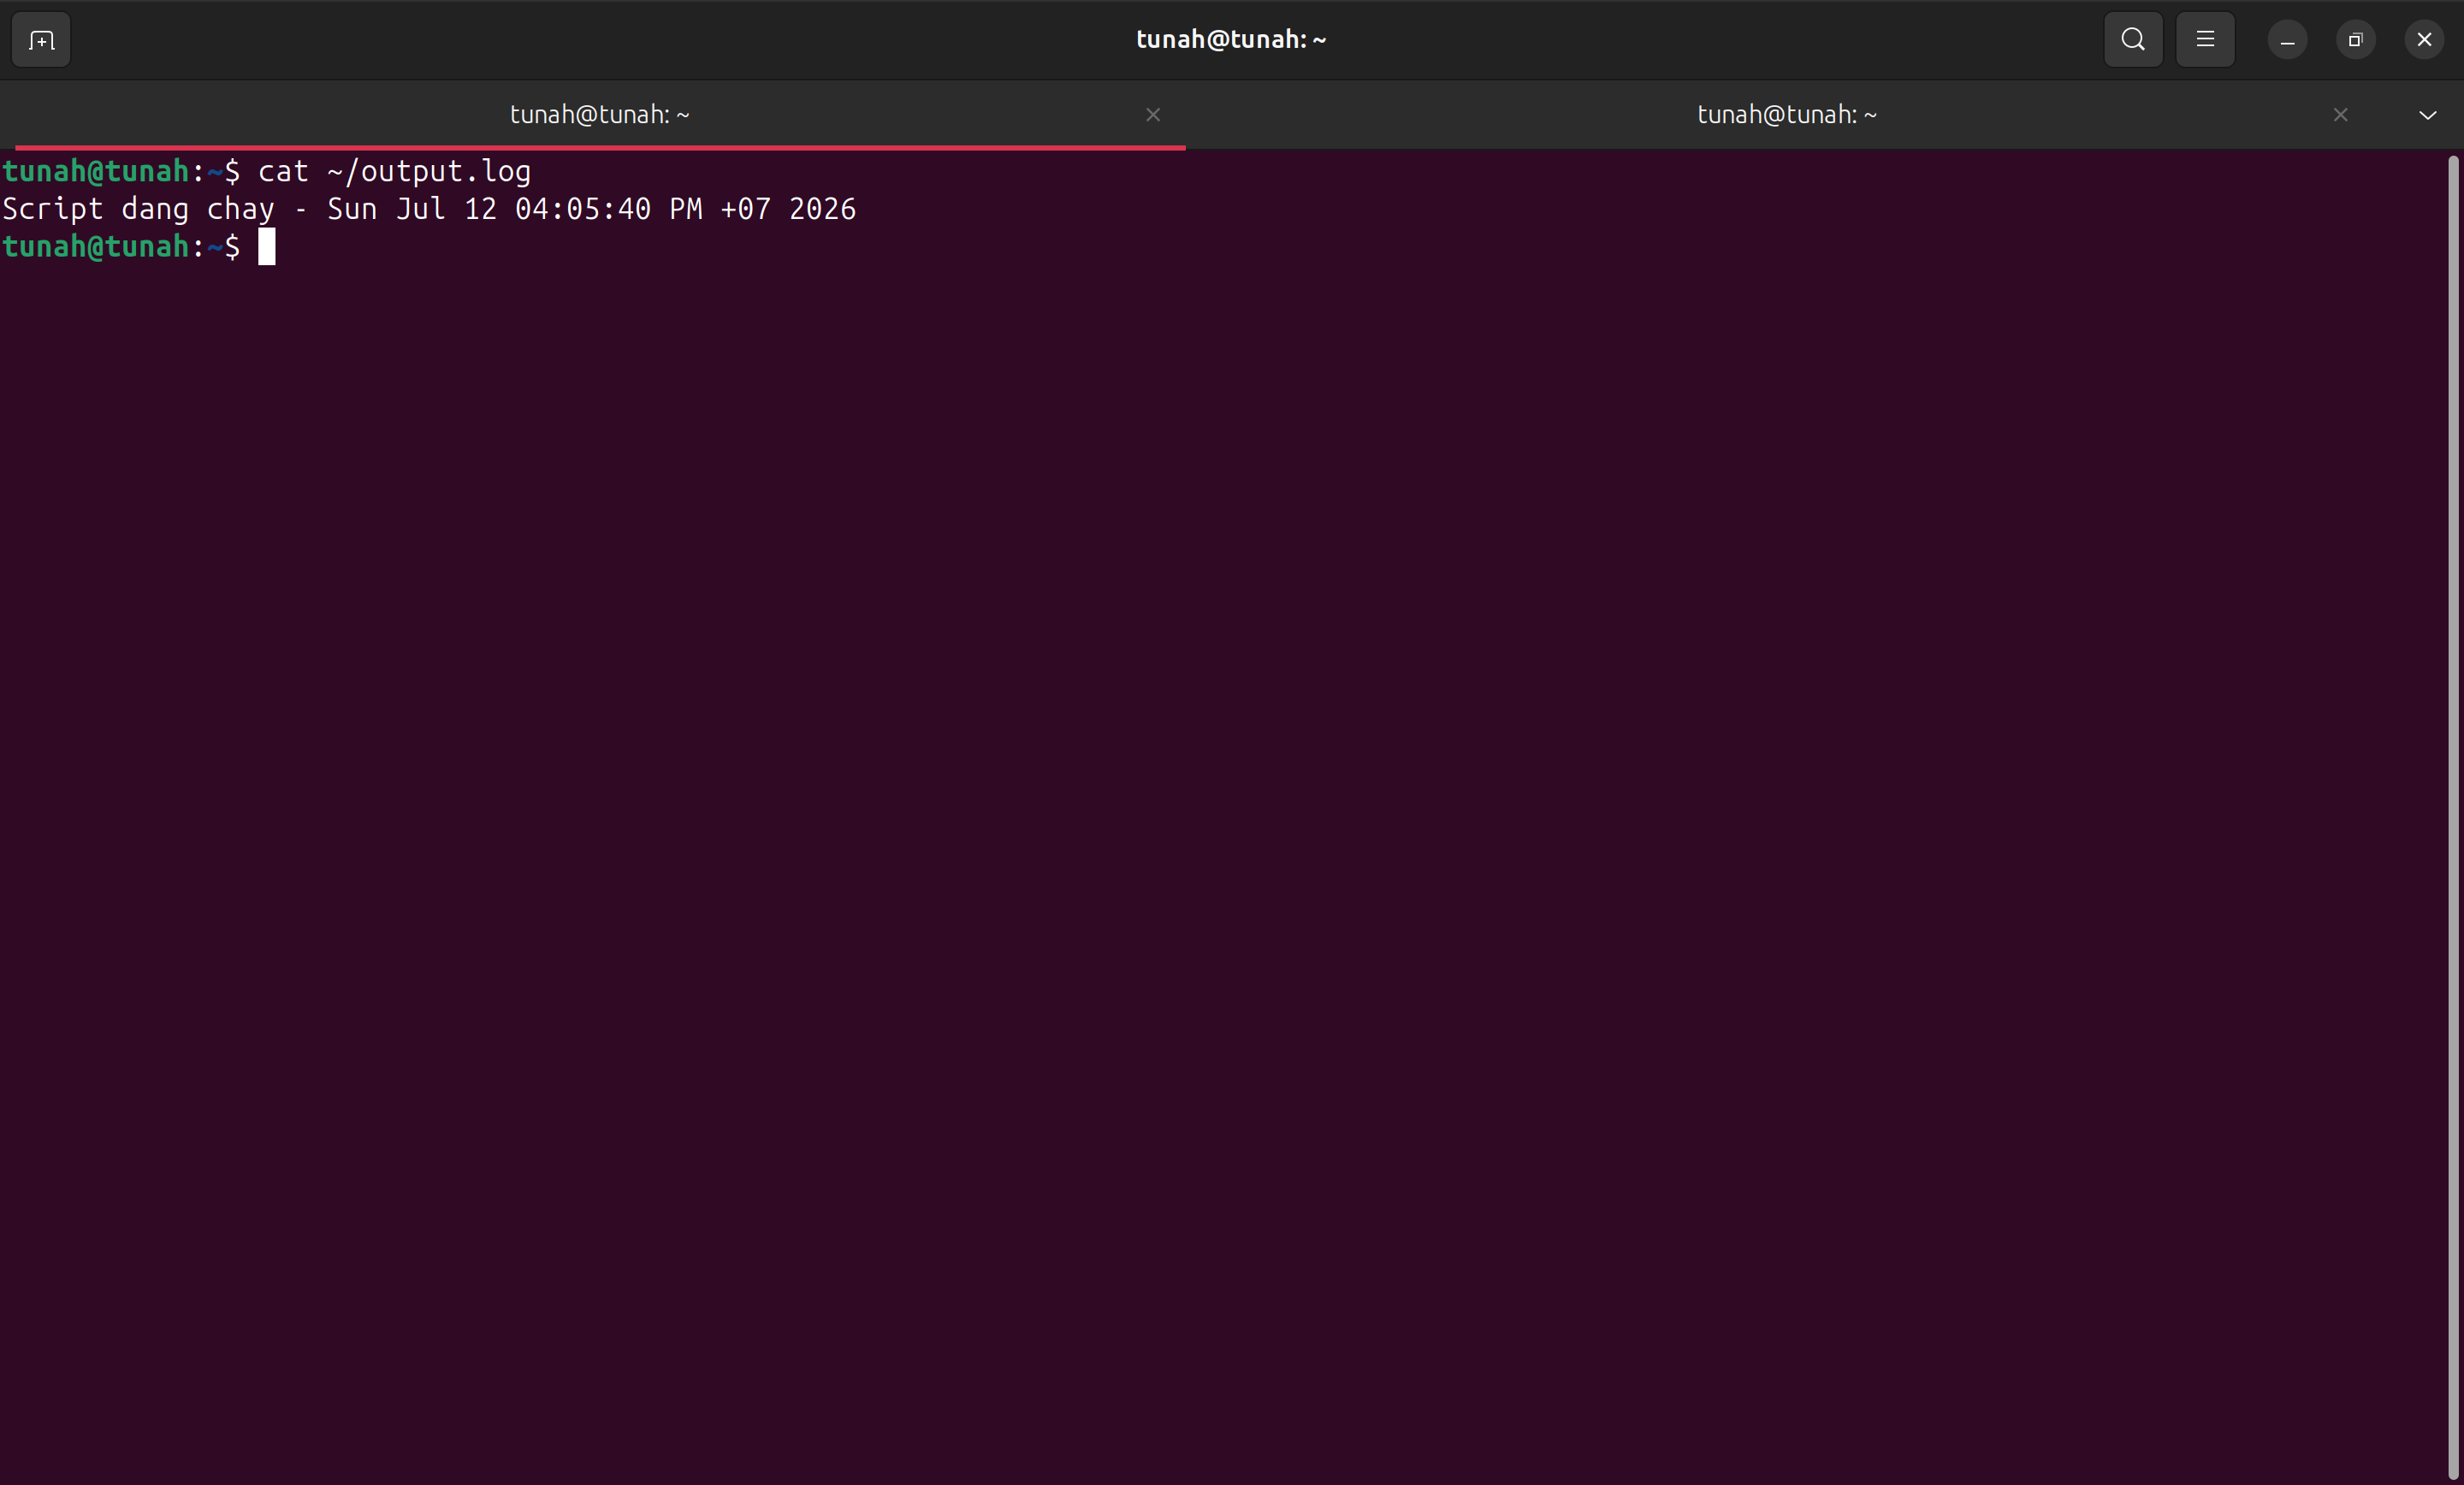
\includegraphics[width=\textwidth]{07/output-log-check.png}
        \caption{Log sinh ra tự động}
    \end{subfigure}
    
    \vspace{0.5cm}
    \begin{subfigure}[b]{0.45\textwidth}
        \centering
        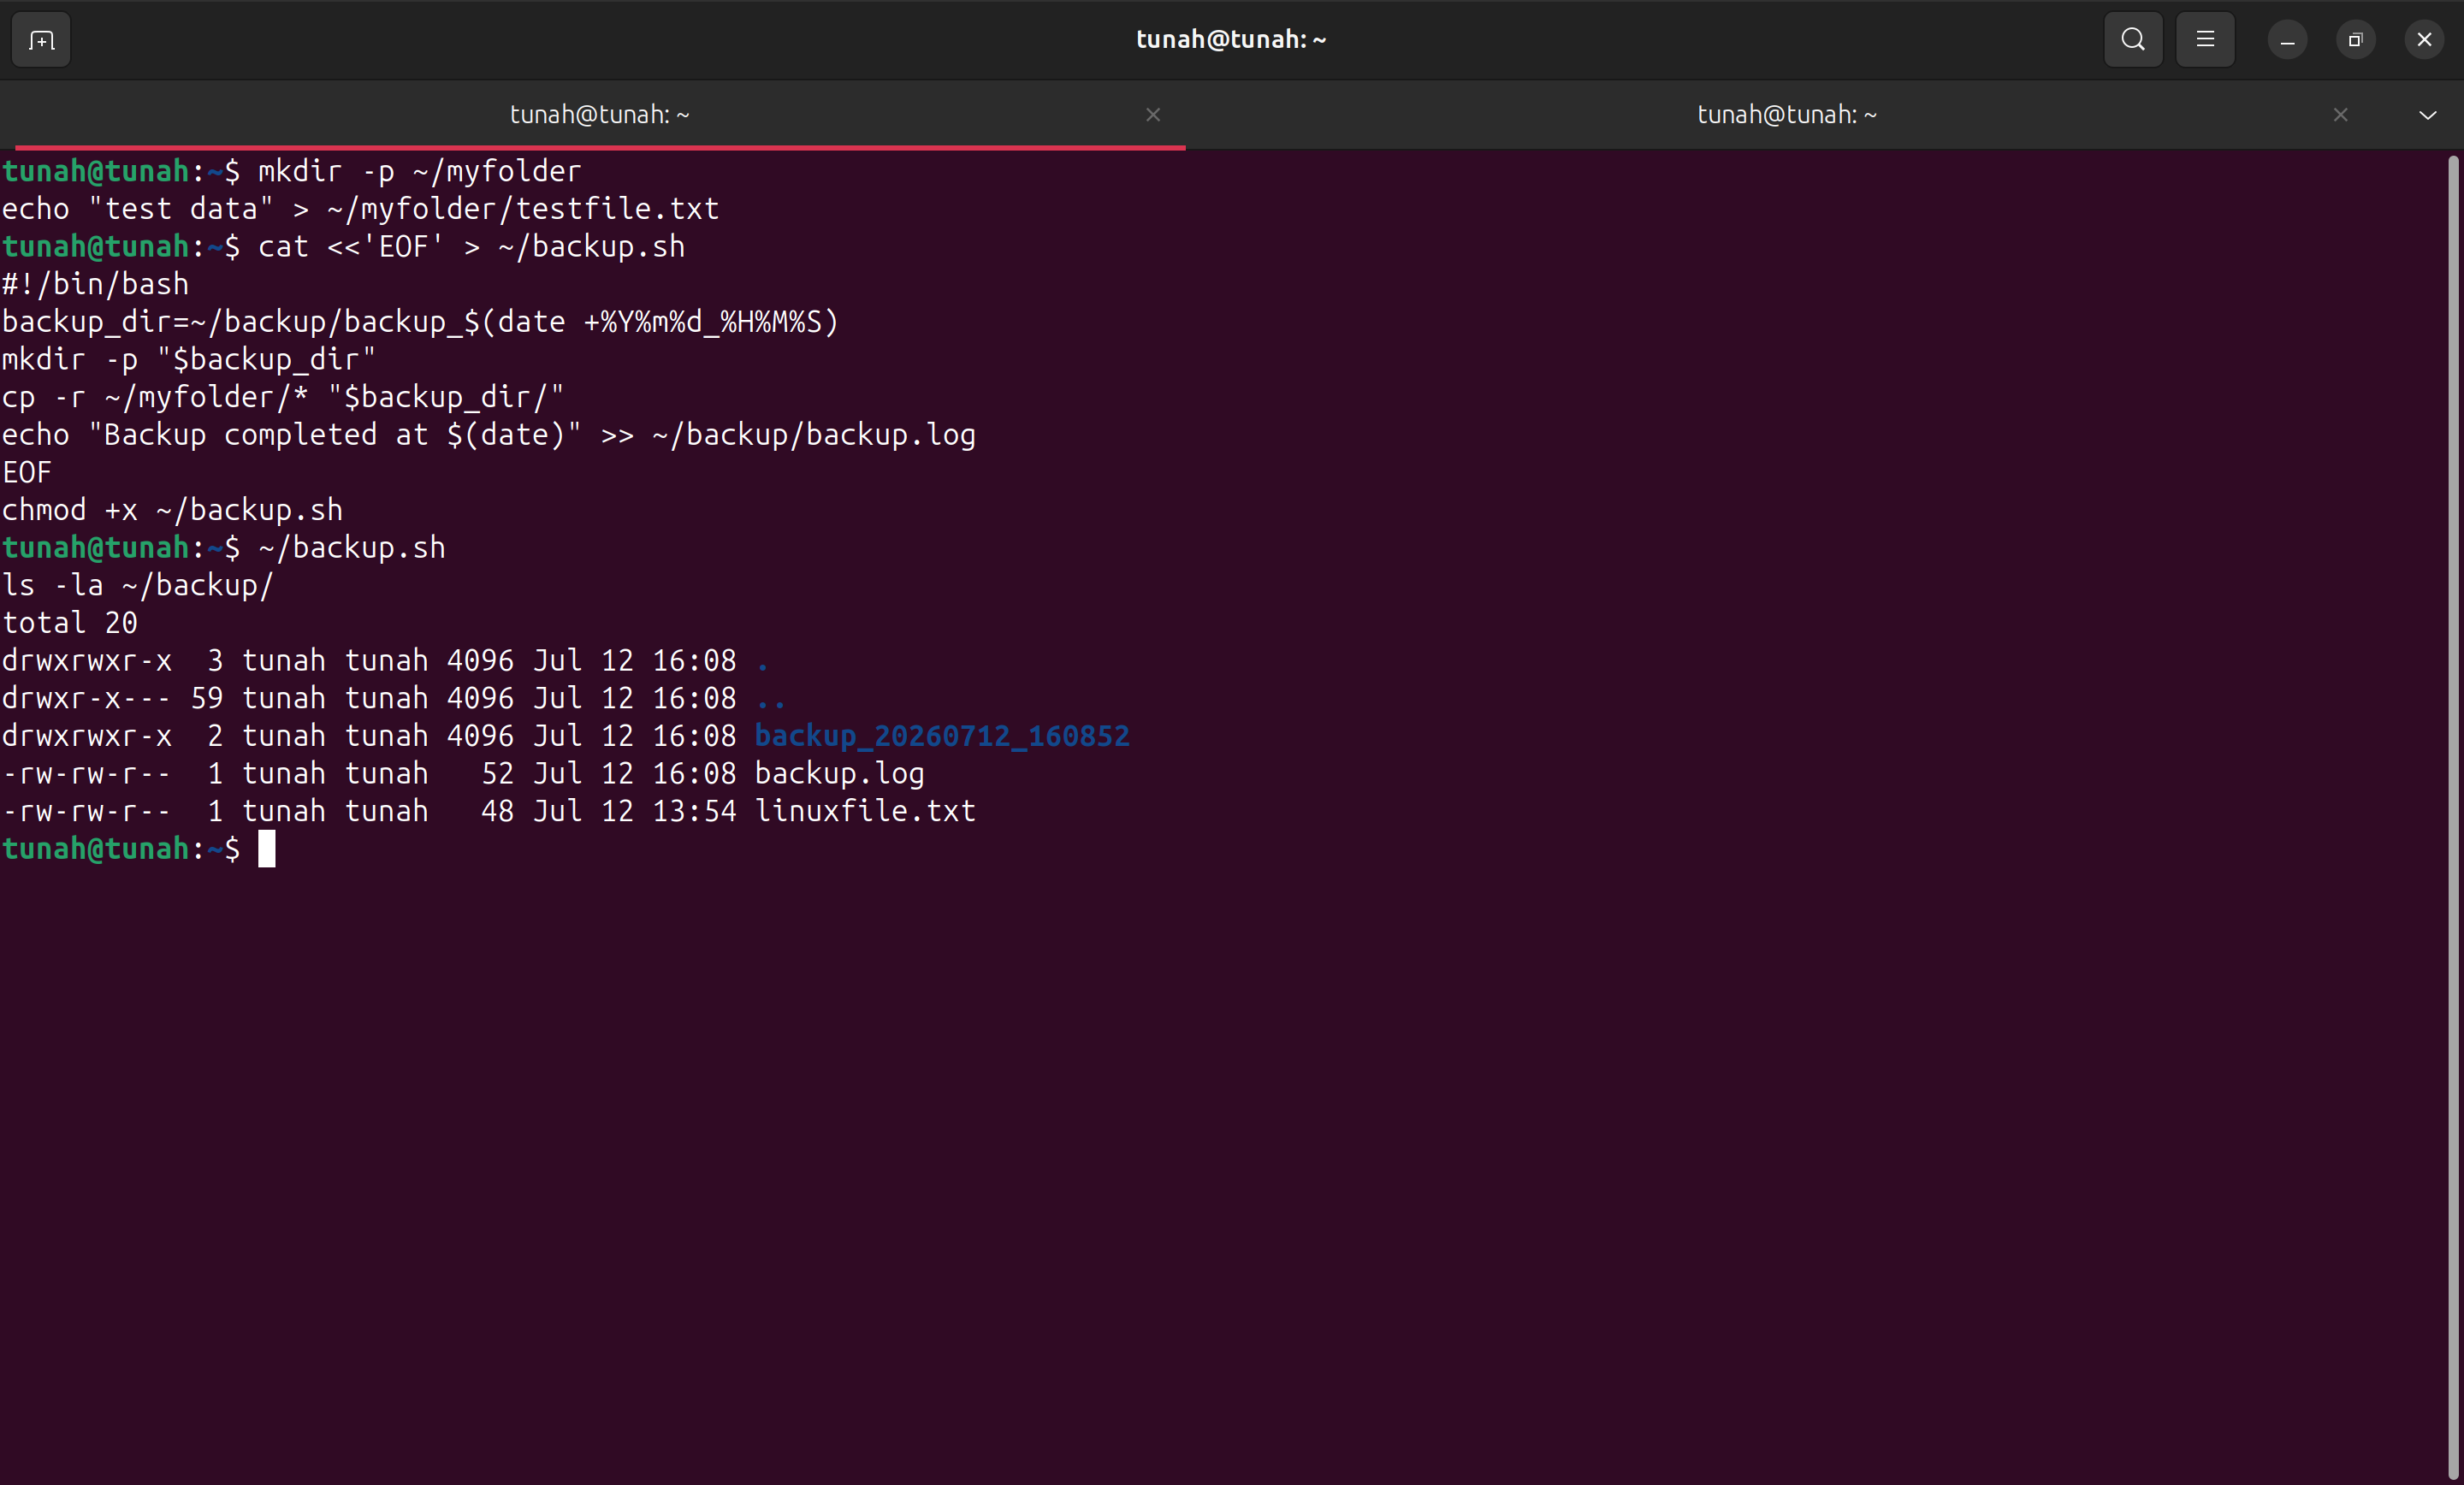
\includegraphics[width=\textwidth]{07/backup-folder-result.png}
        \caption{Thư mục được backup}
    \end{subfigure}
    \hfill
    \begin{subfigure}[b]{0.45\textwidth}
        \centering
        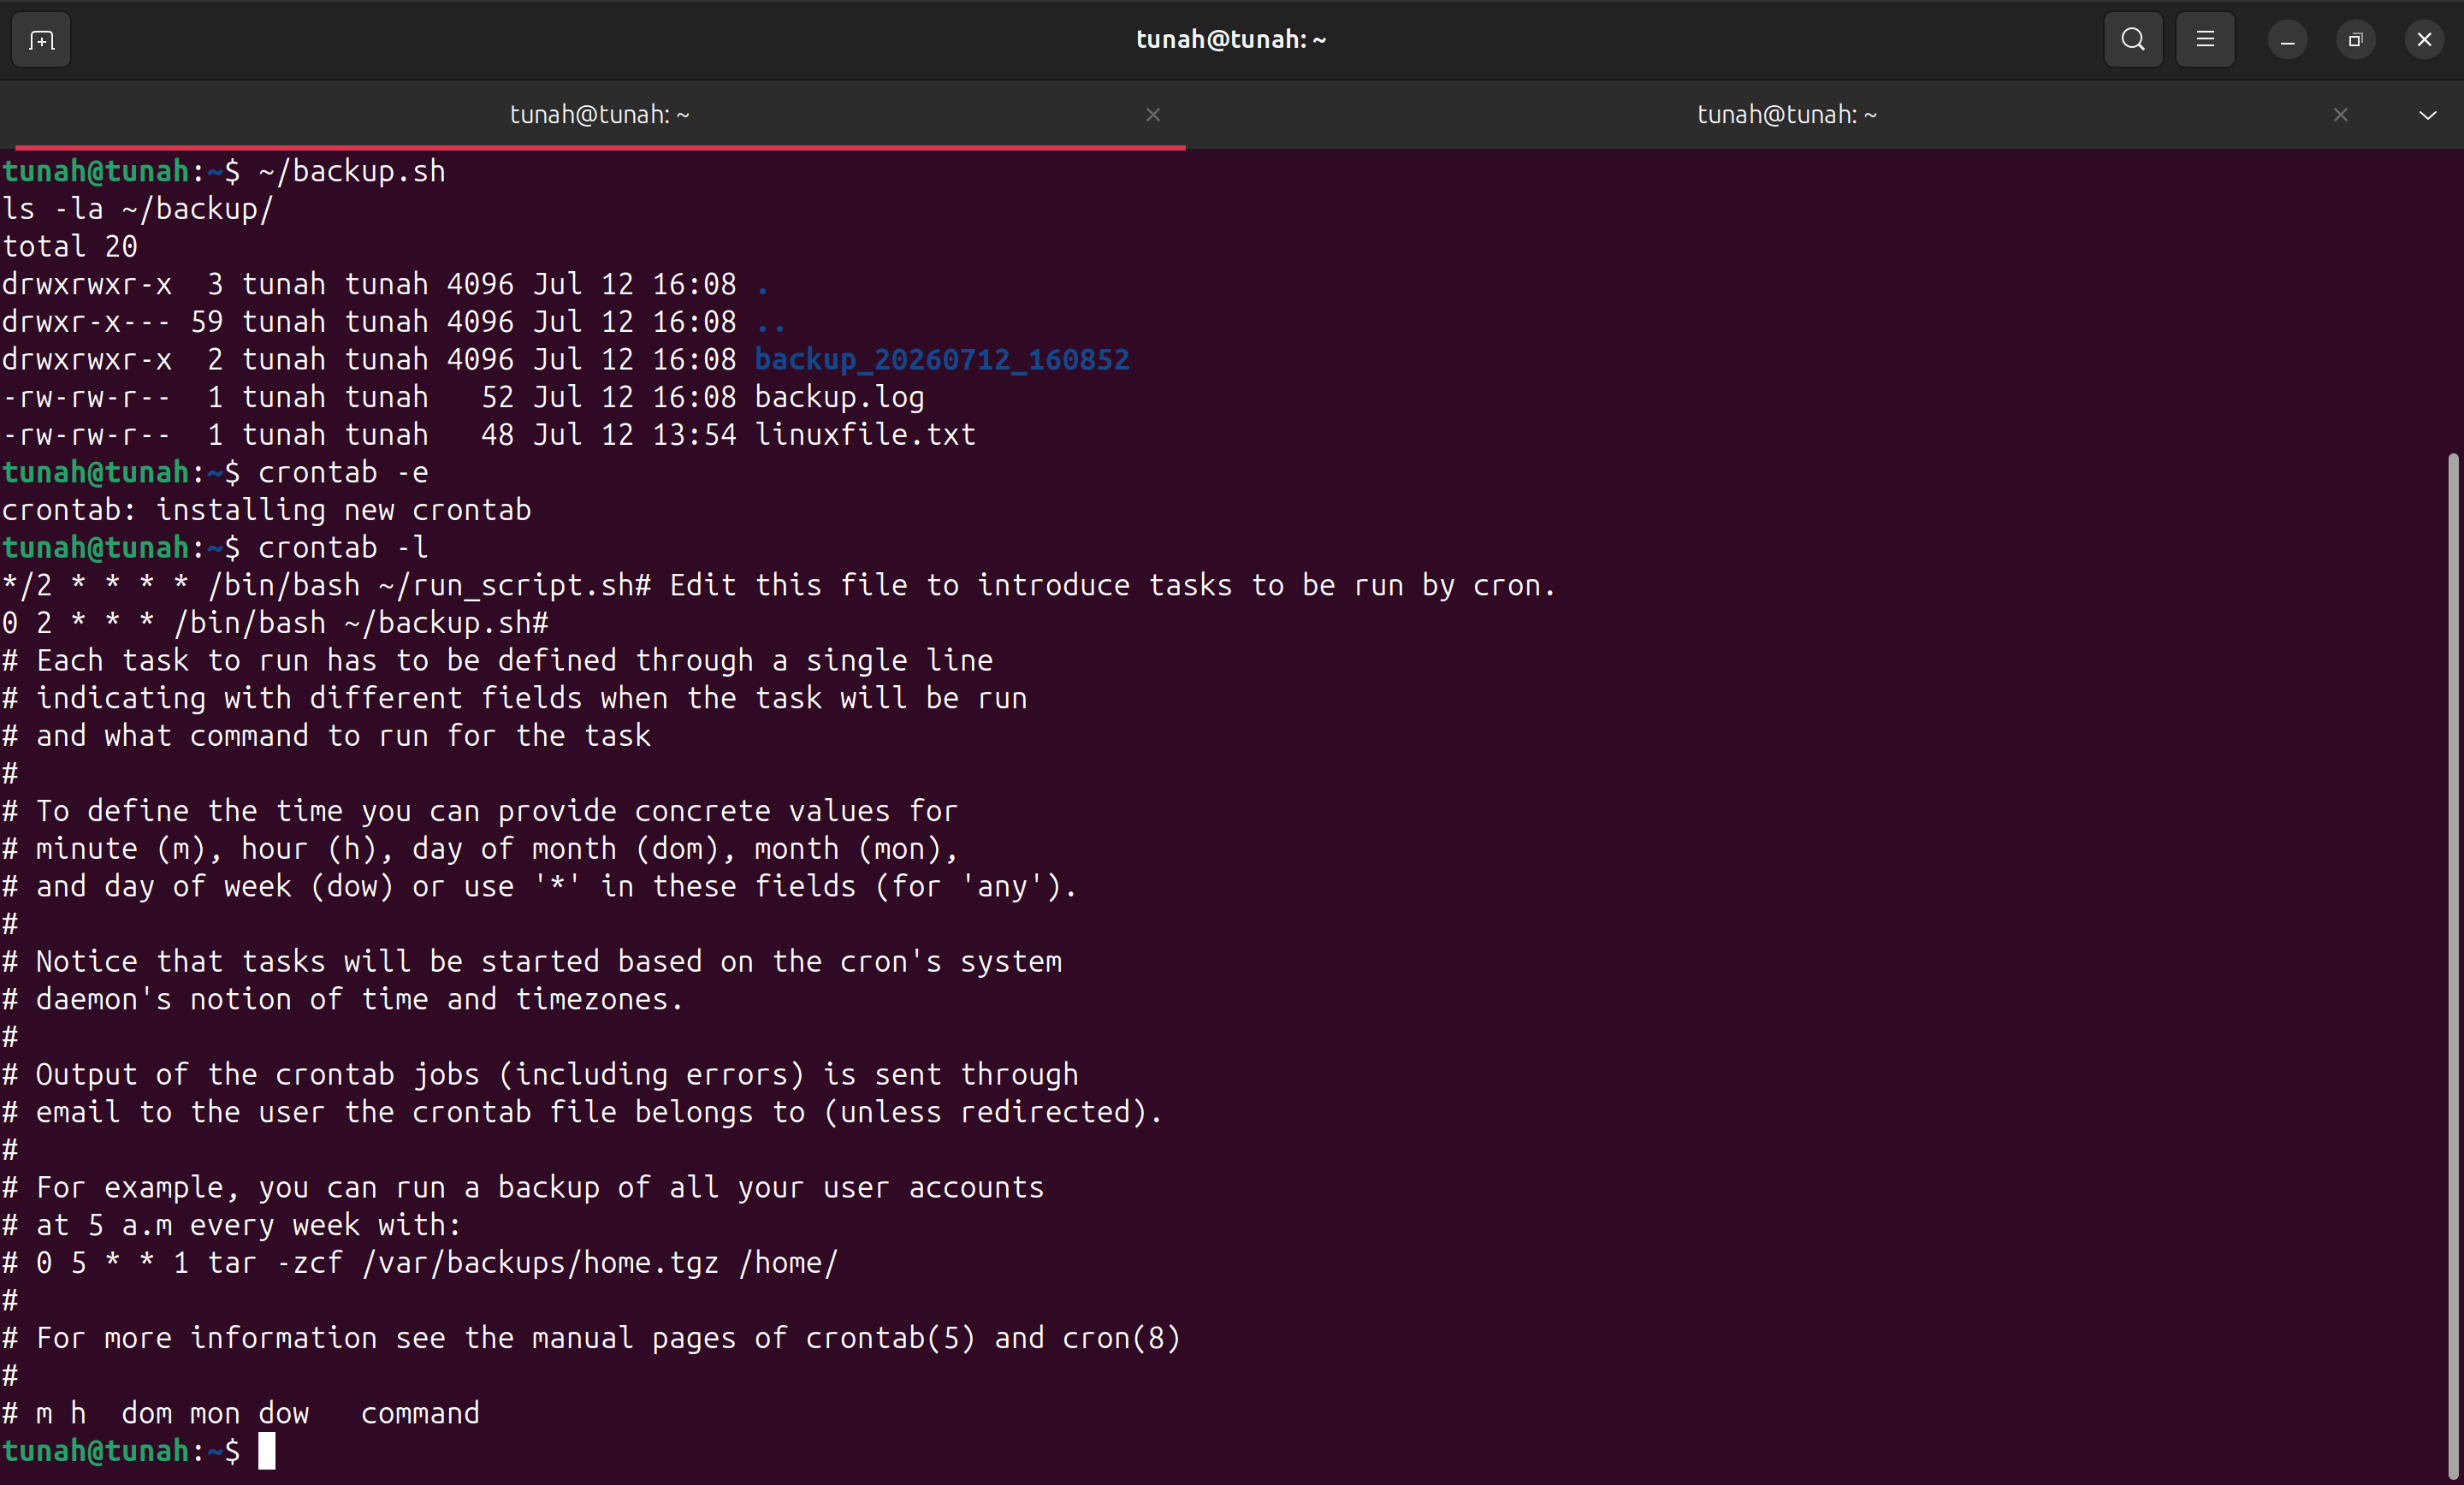
\includegraphics[width=\textwidth]{07/crontab-all-jobs.png}
        \caption{Các cronjob đang chạy}
    \end{subfigure}
    \caption{Lập lịch tự động Cronjob}
\end{figure}


\end{document}
